% A Rubric-Based Survey of Inter-Agent Protocols:
% Industry Standards, Security Posture, Open Problems,
% and Three Co-Designed Protocol Extensions
%
% Target venue: Journal of Artificial Intelligence Research (JAIR).
% Typeset with the official JAIR class from the JAIR AuthorKit. jair.cls
% extends acmart (it loads it with acmlarge, natbib=false, screen), so the
% author blocks, floats, and \cite calls carry over from the previous acmart
% setup. Two things changed with the swap and matter when editing:
%
%   1. Bibliography. natbib is off. References go through biblatex with the
%      biber backend and the acmauthoryear style, so it is \addbibresource
%      plus \printbibliography, not \bibliography plus \bibliographystyle.
%      The build needs biber: `brew install biber`.
%   2. Style is frozen. The AuthorKit README forbids changes to the JAIR
%      style: margins, type sizes, leading, list and paragraph definitions,
%      and manual \vspace. Do not add any here or in preamble.tex.
%
% jair.cls and the three biblatex support files (acmauthoryear.bbx/.cbx,
% acmdatamodel.dbx) are vendored next to this file, copied unmodified from
% JAIR AuthorKit/JAIR_Example_Template/. acmart itself comes from the TeX
% installation. Keeping the JAIR files local means the build does not depend
% on jair.cls reaching CTAN.
%
% Authors: Suranjan Goswami, Manu Ghulyani, Karan Bharadwaj,
%          Roland R. Rodriguez Jr., Faouzi El Yagoubi,
%          Alejandro Quintero, Ranwa Al Mallah
% Cutoff: 2026-Q1
%
% Build: from repo root, `make pdf-latex` (latexmk runs biber automatically)
%        or `make pdf-typst` (fallback via pandoc+typst, no LaTeX required)

% `review` adds line numbers for referees. Drop it for camera-ready and for
% the arXiv posting; scripts/make_arxiv_bundle.sh does that automatically.
\documentclass[manuscript, screen, review]{jair}

% Two builds come out of this file. The JAIR submission carries the journal's
% own furniture: the reference-format block, the associate-editor line, the
% volume and article numbers, the publication date in the page footer, and a
% DOI. The arXiv posting must carry none of it. Every one of those values is a
% placeholder until JAIR assigns it, and a preprint that displays them claims
% a publication that has not happened. Nothing here touches jair.cls, which
% the AuthorKit forbids editing; the overrides are applied from this file.
%
% scripts/make_arxiv_bundle.sh flips this to \arxivtrue. Leave it false in the
% repository so `make pdf-latex` builds the submission version.
\newif\ifarxiv
\arxivfalse

\setcopyright{cc}

\ifarxiv
  % No DOI, and no ACM/JAIR reference-format block or associate-editor line.
  % printacmref=false suppresses both, since jair.cls prints them together.
  \acmDOI{}
  \settopmatter{printacmref=false}
  % The page-1 copyright block prints \@formatdoi unconditionally, so an empty
  % DOI renders as a bare "doi:" with nothing after it. Print nothing when the
  % argument is empty, and behave as before when it is not. This affects the
  % topmatter only; bibliography DOIs come from biblatex, not from this macro.
  % The argument arrives as the macro \@acmDOI rather than as its text, so the
  % emptiness test has to expand it first.
  \makeatletter
  \def\@formatdoi#1{%
    \edef\jair@doitest{#1}%
    \ifx\jair@doitest\@empty\else
      \textsc{doi:} \href{https://doi.org/#1}{#1}%
    \fi}
  \makeatother
\else
  \acmDOI{10.1613/jair.1.xxxxx}
  % Assigned by JAIR, not by the authors. The placeholders below are the
  % AuthorKit's own defaults and get replaced from the acceptance
  % correspondence. \JAIRTrack is empty because this is a regular submission
  % and not part of a special track; jair.cls suppresses the line when it is.
  \JAIRAE{Insert JAIR AE Name}
  \JAIRTrack{}
\fi

\acmVolume{1}
\acmArticle{1}
\acmMonth{1}
\acmYear{2026}

% jair.cls sets the running footer to "Journal of Artificial Intelligence
% Research, Vol. 1, Article 1. Publication date: January 2026." from its own
% \AtBeginDocument. This hook runs after the class's, so it wins. The arXiv
% version keeps a bare page number and asserts no venue or date.
\ifarxiv
  \AtBeginDocument{%
    \fancyfoot{}%
    \fancyfoot[C]{\footnotesize\thepage}%
    \fancypagestyle{firstpagestyle}{%
      \fancyhf{}%
      \fancyfoot[C]{\footnotesize\thepage}%
    }%
  }
\fi

\RequirePackage[
  datamodel=acmdatamodel,
  style=acmauthoryear,
  backend=biber,
  giveninits=true,
  uniquename=init
  ]{biblatex}

\renewcommand*{\bibopenbracket}{(}
\renewcommand*{\bibclosebracket}{)}

\addbibresource{../refs/references.bib}

% Preamble: shared packages and custom macros.

\usepackage{booktabs}
\usepackage{colortbl}
\usepackage{xcolor}
\usepackage{tikz}
\usepackage{pgfplots}
\pgfplotsset{compat=1.18}
\usepackage{microtype}
\usepackage{longtable}
\usepackage{array}

% Rubric axis macro (italicized + indexable). Used throughout sections 5 to 7.
\newcommand{\rubricAxis}[1]{\textit{#1}}

% Protocol badge (colored chip). Used in tables and inline references.
\newcommand{\protocolBadge}[1]{\textsc{#1}}

% Heatmap color palette (used in Table 1 + Figures 5 and 6).
\definecolor{HeatLow}{HTML}{f7fbff}
\definecolor{HeatMidLow}{HTML}{c6dbef}
\definecolor{HeatMid}{HTML}{6baed6}
\definecolor{HeatMidHigh}{HTML}{2171b5}
\definecolor{HeatHigh}{HTML}{08306b}

% Companion repository URL. JAIR review is single-blind, so the link is
% printed in the submission. Defined once here so a rename edits one line.
% The repository exists under this name; it is private until submission.
\newcommand{\companionrepo}{\url{https://github.com/suranjan-nasiko/inter-agent-protocol-survey}}

% Score formatting (ordinal 0 to 3 with anchored descriptors).
\newcommand{\score}[1]{\textbf{#1}}


\begin{document}

% JAIR requires a short title for the page headers, since the full one is
% three lines. The line breaks the full title used under acmart are gone:
% the AuthorKit says not to insert breaks in a title, and jair.cls wraps it.
\title[A Rubric-Based Survey of Inter-Agent Protocols]{A Rubric-Based Survey
  of Inter-Agent Protocols: Industry Standards, Security Posture, Open
  Problems, and Three Co-Designed Protocol Extensions}

\author{Suranjan Goswami}
\authornote{Corresponding Author.}
\affiliation{%
  \institution{Nasiko Labs}
  \country{India}
}
\email{suranjan_arcade@yahoo.co.in}

\author{Manu Ghulyani}
\affiliation{%
  \institution{Nasiko Labs}
  \country{India}
}
\email{manughulyani@gmail.com}

\author{Karan Bharadwaj}
\affiliation{%
  \institution{Nasiko Labs}
  \country{USA}
}
\email{karan@nasiko.com}

% Details taken from the public record only, pending his own confirmation.
% Name string, affiliation and email are exactly as he self-published them on
% the title page of arXiv:2601.14567v2, the agent:// scheme paper cited here
% as \cite{agent_uri_scheme}. That page reads "Roland R. Rodriguez, Jr. /
% Independent Researcher / rrrodzilla@proton.me", and its footnote 1 names
% the same address as the contact point. No country appears on that page;
% United States comes from his publicly listed Govcraft office in Corpus
% Christi, Texas (govcraft.ai). The suffix comma is braced so acmart does
% not read it as an author separator.
\author{Roland R. Rodriguez, {Jr.}}
\affiliation{%
  \institution{Independent Researcher}
  \country{United States}
}
\email{rrrodzilla@proton.me}

\author{Faouzi El Yagoubi}
\affiliation{%
  \institution{Polytechnique Montr\'eal}
  \city{Montr\'eal}
  \state{Qu\'ebec}
  \country{Canada}
}
\email{faouzi.el-yagoubi@polymtl.ca}

\author{Alejandro Quintero}
\affiliation{%
  \institution{Polytechnique Montr\'eal}
  \city{Montr\'eal}
  \state{Qu\'ebec}
  \country{Canada}
}
\email{alejandro.quintero@polymtl.ca}

\author{Ranwa Al Mallah}
\affiliation{%
  \institution{Polytechnique Montr\'eal}
  \city{Montr\'eal}
  \state{Qu\'ebec}
  \country{Canada}
}
\email{ranwa.al-mallah@polymtl.ca}

% JAIR asks for a short author list for the running head, and strongly
% recommends an \orcid per author. Neither the Nasiko Labs authors nor
% Rodriguez has supplied an ORCID, and the Polytechnique Montreal authors
% joined too recently to have been asked, so no \orcid lines appear above.
% They are not invented here: a wrong ORCID resolves to a real stranger.
% Collect all seven before camera-ready; the README tracks this.
\renewcommand{\shortauthors}{Goswami et al.}

% =====================================================================
% Reserved author slot (1 remaining of the 3 originally held).
% Slots six and seven went to Alejandro Quintero and Ranwa Al Mallah
% (Polytechnique Montreal), named as co-authors in Faouzi El Yagoubi's
% reply of 2026-09-09.
%
% Kept commented so the circulating draft's title page does not show
% placeholder names. The block needs all four fields, or acmart emits
% a missing-metadata warning.
% =====================================================================
% \author{Author Eight}
% \affiliation{%
%   \institution{TODO: affiliation}
%   \country{TODO: country}
% }
% \email{TODO@example.org}

% JAIR uses a structured abstract: Background, Objectives, Methods, Results,
% Conclusions, each introduced by a bold run-in label. The content is the same
% claim set as the prose abstract this replaced, redistributed under the five
% headings, with the honesty disclosures (single rater, no inter-rater
% statistic, sketches not standards) kept where a reader meets them early.
% Note that the arXiv abstract in manuscript/arxiv-abstract.txt is a third,
% independent text under a 1920-character limit. Changing a claim here means
% changing it there too; see manuscript/arxiv-abstract-NOTES.md.
\begin{abstract}
{\bf Background:}
The 2024 to 2026 period has produced an explosion of inter-agent protocols.
Google A2A, Anthropic MCP, IBM ACP, Cisco AGNTCY/SLIM, ANP, Coral, LOKA,
ACNBP, AP2, Visa Trusted Agent Protocol, ERC-8004, and UCP each address
overlapping fragments of the multi-agent coordination problem. Four broad
surveys already exist. What is missing is a principled basis for comparing
them.

{\bf Objectives:}
We set out to make the comparison auditable rather than narrative. That means
one rubric applied uniformly to every protocol, one recorded reason per
score, and an agenda of open problems that follows from the resulting gaps
rather than from opinion.

{\bf Methods:}
We contribute a uniform \emph{rubric} of ten evaluation axes. The axes span
discovery, identity, authorization, transport, task model, async, multi-modal
handling, security threat surface, semantic interoperability, and governance.
We survey thirteen protocols across three architectural layers (tool-binding,
peer-messaging, commerce-settlement). We score the eight tool-binding and
peer-messaging protocols against the full rubric. The five
commerce-settlement protocols are compared on a separate structural basis,
because the rubric's task, transport, and threat axes do not apply to a
settlement envelope. Scores come from a single rater reading each
specification under stated calibration rules. We report an auditable change
history over a machine-readable score file, and no inter-rater agreement
statistic.

{\bf Results:}
No protocol scores uniformly high, and the rubric shows why: the
contemporary protocols specialize into mutually exclusive strengths. None
combines a deployed task model with a decentralized identity model. The
authorization axis is the sharpest result. Its top level is empty across all
eight scored protocols, so no surveyed peer-messaging protocol offers a
standardized delegation credential that a downstream agent can verify. The
gap is universal rather than near-universal, and it holds even for the
protocol with the widest threat coverage in the set. We also map industry
adoption across enterprise SaaS, agentic commerce and payments, healthcare,
and finance, and we survey the emerging security and threat-modeling
literature.

{\bf Conclusions:}
The gaps identify the work of the next standardization cycle, and we propose
three co-designed protocol extensions against them. \emph{OWA} is a URI
scoping scheme. It adds an explicit \emph{workspace} tier between the
organizational trust root and the agent identifier. \emph{ACSP} is a sibling
envelope that records the sender's declared context-selection step: which
candidate items were considered, which were kept, which were dropped, under
which token budget and optimisation objective. Its signed wire-level audit
log carries observable invariants the receiver can verify. \emph{AGRP} is a
normative A2A envelope. It binds every cross-boundary message to a
classification-label set and a commitment-bearing redaction log on the spans
the egress filter claims to have touched. It also requires either a signed
Tier~1 enforcement claim or independently verified Tier~2 evidence. The three
close a single loop, naming to selection to attestation, that no contemporary
protocol provides. All three are positioned as specification-sketch
contributions for the next AAIF and W3C revision cycles rather than as
validated standards.
\end{abstract}

% JAIR Note from the AuthorKit: do not include ACM CCS Concepts or Keywords.
% The \keywords list that stood here under acmart was removed for that reason.

% Placeholder submission date. JAIR fills the accepted date at production;
% \received[accepted]{} is added then, not now. The arXiv posting omits it:
% a received date is the journal's record of a submission, and printing it on
% a preprint asserts a review process the preprint is not part of. arXiv
% stamps its own submission date. \ifarxiv is set in main.tex.
\ifarxiv\else
  \received{14 September 2026}
\fi

\maketitle

% Cutoff date declared on page 1, per the differentiation strategy (R1, R3).
\noindent\textbf{Note on scope.} Specifications and literature surveyed
up to 2026-Q1; later developments may be referenced in footnotes but
are not exhaustively covered.


% A survey this long is navigated, not read front to back, so it carries a
% contents list. Depth 2 (sections + subsections) lists all 14 sections and 64
% subsections. Depth 3 would add 35 subsubsections, most of them inside the
% rubric axis walkthrough and the three proposals, and push the list past three
% pages without adding a landmark a reader looks for.
\setcounter{tocdepth}{2}
\clearpage
\tableofcontents
\clearpage

\section{Introduction}
\label{sec:intro}

\subsection{Motivation}
\label{sec:intro:motivation}

Between April 2025 and the end of 2025-Q1 2026, the inter-agent
interoperability landscape passed through what is, by any reasonable
counting, a Cambrian phase. Google launched the Agent2Agent (A2A)
protocol in April 2025 and donated it to the Linux Foundation later in
the year~\cite{spec_a2a, lf_aaif}. Anthropic's Model Context Protocol
(MCP), introduced in late 2024, became the de-facto tool-binding
standard and was adopted by every major model vendor within
months~\cite{spec_mcp}. The Agent Network Protocol (ANP) published its
white paper in August 2025~\cite{spec_anp}. IBM's ACP/BeeAI,
Cisco-led AGNTCY and its SLIM secure messaging layer, Coral Protocol,
the LOKA framework, and the Agent Capability Negotiation and Binding
Protocol (ACNBP) all reached public specifications within the same
twelve-month window~\cite{spec_coral, spec_loka, spec_acnbp}.
In parallel, the agentic-commerce stack took shape: Google's Agent
Payments Protocol (AP2), Visa's Trusted Agent Protocol (TAP),
Mastercard's Agent Pay, and the Ethereum community's ERC-8004.
A fifth specification, the Universal Commerce Protocol (UCP),
followed at the start of 2026 and covers the commerce transaction
around the payment rather than the payment itself.
These specifications introduced a third architectural layer. It is
concerned not with tool invocation or peer messaging but with
cryptographically-attested commerce settlement on behalf of an
agent principal.

Four broad surveys of inter-agent protocols already
exist~\cite{yang2025survey, ehtesham2025interop, kong2025communication,
commcentric2025survey}. They establish taxonomies and identify research
directions. Kong et al.~\cite{kong2025communication} additionally
provide a deep security analysis in 48 pages and 18 figures. None,
however, proposes a normalized scoring rubric that could be applied
uniformly across the protocol landscape; none covers the
agentic-commerce stack at the spec level; none maps industry adoption
by vertical; and none ships a machine-readable companion artifact that
remains usable as protocol versions drift during the typical 6 to 9
month review cycle of an archival journal. The contribution gap
motivating this survey is
precisely that intersection:
\emph{a rubric that scores existing specs uniformly, applied across the
full inter-agent protocol landscape including commerce, grounded in
named industry deployments, and re-runnable from a machine-readable
score file.} Re-runnable is a claim about the artifact, not about
scoring reliability: every score here is one rater's, and
\S\ref{sec:rubric:calibration} states what agreement evidence that
does and does not give us.

The closest precedent in method predates these surveys. Chopra,
Christie, and Singh define criteria for evaluating communication
protocol languages and compare five academic languages against
them~\cite{chopra2020protocol}. Those languages are formal notations
for specifying multiagent interactions. The protocols surveyed here
are industry specifications that deployed LLM agents use. They raise
questions of identity, authorization, and governance that lay outside
that study's scope, and the rubric of \S\ref{sec:rubric} adds axes
for them.

\subsection{Why now: the 2024 to 2026 protocol explosion}
\label{sec:intro:whynow}

Three forces converged to produce the protocol explosion that this
survey records. First, the maturation of frontier LLMs as tool-using
agents created an immediate demand for a standardized
context-injection contract, which MCP filled. Second, multi-agent
deployment patterns made it apparent that a tool-binding protocol
alone was insufficient. Those patterns include supervisor-and-worker,
peer-to-peer specialist teams, and long-running task delegation
across organizational boundaries. Peer-messaging protocols (A2A,
ACP, ANP, AGNTCY, Coral) emerged within months of MCP's
stabilization. Third, the
rise of agent-initiated transactions on behalf of human principals
exposed an unmet need for cryptographically verifiable
authorization, leading the major card networks and a parallel
on-chain effort (ERC-8004) to specify what we treat in this survey
as the commerce-settlement layer of inter-agent coordination.

The result is a landscape with substantial overlap but no clear
ranking: a practitioner choosing among A2A, ANP, and Coral for a
multi-agent deployment finds extensive specifications but no
neutral basis for comparison. The four prior surveys provide
taxonomies and qualitative observations; this survey provides a
normalized scoring framework, anchored against the eight
protocols of the tool-binding and peer-messaging layers and
applied to thirteen protocols in total across the three layers,
alongside an industry
adoption synthesis and a security threat-coverage matrix.

\subsection{Contributions}
\label{sec:intro:contributions}

This survey makes seven distinct contributions.
Contributions C1 to C4 are survey contributions, each of
which is absent from the four prior surveys of the
landscape~\cite{yang2025survey, ehtesham2025interop,
kong2025communication, commcentric2025survey}.
Contributions C5, C6, and C7 are protocol-design
proposals derived from the open-problems agenda the
survey identifies; they are narrowly-scoped extensions
to the contemporary protocol stack, not free-standing
protocols, and they are presented in
\S\ref{sec:proposals} after the survey is complete.

\paragraph{Contribution C1: A uniform 10-axis rubric.}
We propose an evaluation rubric of ten axes. The axes are Discovery
and Registry
Model, Identity and Authentication, Authorization and Delegation,
Transport and Wire Format, Task and Conversation Model, Async and
Long-Running Operations, Multi-Modal Content Handling, Security
Threat Surface, Semantic Interoperability, and Governance / License /
Observability. We apply the ten axes to the eight tool-binding and
peer-messaging protocols (\S\ref{sec:rubric};
Table~\ref{tab:rubric-matrix}), and compare the four
commerce-settlement protocols on the structural axes that do apply to a
settlement envelope (Table~\ref{tab:commerce-stack}). Every rubric score
in this survey is therefore one of eight protocols, and the count of
thirteen refers to the surveyed set. Seven axes use
anchored ordinal scoring (0 to 3) with explicitly named anchor
descriptors per level; one axis (Transport) is a structured
tuple to avoid the false precision of ordinal scoring over a
configuration space; one axis (Security) is a count over a fixed
twelve-item threat catalog; and one axis (Governance / License /
Observability) is a composite triple of categorical steward,
license identifier, and 0 to 3 observability score. Prior surveys propose taxonomies
(Yang~\cite{yang2025survey}, Kong~\cite{kong2025communication}) or
adoption roadmaps (Ehtesham~\cite{ehtesham2025interop}) but no
normalized scoring framework that lets a reader rank a new protocol
against existing ones.

\paragraph{Contribution C2: First-class treatment of the
agentic-commerce stack.}
We treat AP2, Visa TAP, Mastercard Agent Pay, ERC-8004, and UCP as a
first-class third architectural layer of inter-agent coordination,
alongside tool-binding (MCP and its descendants) and peer-messaging
(A2A, ANP, ACP, AGNTCY, Coral, LOKA, ACNBP). Section~\ref{sec:industry-protocols}
analyzes the commerce stack at the spec level. That analysis covers
its intent-mandate-receipt envelope, its principal-delegation chain
semantics, its on-chain versus off-chain settlement models, and
the cross-network interoperability work underway in the Agentic
AI Interoperability Foundation~\cite{lf_aaif}. It also covers UCP's
alternative to that harmonisation: fix the transaction layer above
the settlement protocols and treat the mandate as a negotiated
extension. No prior survey
covers the commerce-settlement layer at this depth; Yang and
Kong predate its emergence; Ehtesham's four-protocol scope omits
it; the communication-centric survey~\cite{commcentric2025survey}
treats payments as out of scope.

\paragraph{Contribution C3: Industry adoption mapped by vertical.}
Section~\ref{sec:adoption} and Table~\ref{tab:industry-adoption}
synthesize industry adoption across four verticals: enterprise
SaaS, agentic commerce and payments, healthcare, and finance. The
synthesis names production deployments rather than treating protocols
in the abstract. We track which protocols are shipping in identifiable
products, which carry pilot-stage announcements, and which remain
research artifacts. Prior surveys do not provide this mapping; the
absence is particularly notable in Yang and Kong, where adoption
is treated only at the level of which vendor designed which
specification.

\paragraph{Contribution C4: A machine-readable companion artifact.}
We ship a companion repository (\companionrepo) carrying \texttt{protocol-scores.yaml}
(the source of truth behind Table~\ref{tab:rubric-matrix},
Figure~\ref{fig:heatmap}, and Figure~\ref{fig:radar}), the threat
coverage and adoption matrices as YAML, and the scripts that
regenerate the tables and figures built from them. This artifact addresses the
staleness risk that broadly threatens any protocol survey across
a 6 to 9 month review cycle: scores remain re-runnable as protocol
versions drift, and a reader can fork the YAML to score a ninth
protocol without re-implementing the comparison. Prior surveys do
not provide machine-readable comparison artifacts. Its contents
and license terms are listed in the reproducibility checklist of
Appendix~\ref{sec:appendix:repro}.

\paragraph{Contribution C5: The OWA scoping scheme.}
We propose a three-tier \emph{org / workspace / agent} URI naming
scheme (\S\ref{sec:proposals:owa}) that extends the
\texttt{agent://} URI scheme of Rodriguez~\cite{agent_uri_scheme}
with an explicit workspace tier between the organizational trust
root and the capability path. The workspace tier is missing from
every contemporary identifier scheme: \texttt{agent://}, the
Agent Name Service IETF draft~\cite{ans_ietf}, A2A AgentCard URIs,
W3C DIDs, and Ruflo's cross-machine federation~\cite{ruflo}.
Yet the empirical reality of enterprise deployments points the
other way (\S\ref{sec:adoption:saas}). Multiple agents with
overlapping capabilities operate under different workspace
governance regimes. OWA names the workspace as a first-class
URI segment, enabling per-workspace policy enforcement, cross-org
trust bootstrap through DNS, and the boundary detection that
Contribution C6 depends on. The proposal addresses P7
(trust-bootstrapping across heterogeneous registries) of the
open-problems agenda (\S\ref{sec:openproblems:trust}).

\paragraph{Contribution C6: The AGRP guardrails envelope.}
We propose a normative envelope extension to A2A
(\S\ref{sec:proposals:agrp}) that wraps every cross-boundary
inter-agent message with classification labels, a
fingerprint-evidenced redaction log, and cryptographic
attestation that an egress filter ran. The envelope is bound to
the sender's OWA identity (Contribution C5), allowing the
receiver to verify the egress-filtering property at the
\emph{message} layer rather than relying on the sending
deployment to enforce it. The proposal is positioned explicitly
as a composition partner with the most-developed deployment-layer
precedent, Pipelock~\cite{pipelock}: the AGRP envelope's
\texttt{mediator\_receipt} field is designed to carry Pipelock
receipts forward, yielding a defence-in-depth deployment of
deployment-layer enforcement plus protocol-layer cross-vendor
verifiability. AGRP addresses three open security problems, as
catalogued in \S\ref{sec:security:open}. They are
O3 (prompt-injection mitigation as spec-level requirement),
O5 (contextual integrity for forwarding), and O6 (side-channel
metadata privacy).

\paragraph{Contribution C7: The ACSP context selection envelope.}
We propose a sibling envelope extension to A2A
(\S\ref{sec:proposals:acsp}) that records the
\emph{declared selection step itself}: which candidate items from
the sender's context pool were considered, which were
kept, which were dropped, under which token budget and
optimisation objective, with a keyed per-candidate
commitment and an attestation chain signed by the
sender's OWA-bound key (Contribution C5). Where AGRP
attests the cleaning of \emph{spans within} forwarded
items, ACSP attests the prior decision of \emph{which
items} crossed the boundary. That is the gap AgentLeak's
output-only audits miss 41.7\% of the
time~\cite{agentleak}. ACSP is positioned as the
protocol-layer answer to the contextual-integrity
question \S\ref{sec:security:privacy} leaves open, and
is anchored on the PACMS~\cite{pacms_cikm_demo} reference
implementation (submodular facility-location selection;
the classical coverage guarantee is not asserted for the
audited token-knapsack implementation without its required
conditions). The three proposals are co-designed: OWA
names the boundary; ACSP selects which items cross it;
AGRP redacts the spans within those items. The triplet
closes the contextual-integrity loop at the wire layer
in a way no contemporary protocol provides.

\subsection{What this survey is not}
\label{sec:intro:notwhat}

The scope of this survey is deliberately bounded, and several
adjacent literatures are explicitly out of frame.

This is \emph{not} a survey of LLM agents or single-agent reasoning
frameworks. AutoGen~\cite{wu2023autogen},
MetaGPT~\cite{hong2024metagpt}, ChatDev~\cite{qian2024chatdev},
CAMEL~\cite{li2023camel}, and their successors
are foundational context for the protocols we evaluate, but they
are not themselves subjects of the rubric and do not appear in
Table~\ref{tab:rubric-matrix}.

This is \emph{not} a survey of multi-agent reinforcement learning.
Where coordination questions overlap (e.g., consensus, role
assignment), we cite the MARL literature for context only.

This is \emph{not} a re-derivation of the security threat
literature. The deep security analysis of inter-agent communication
already exists in Kong et al.~\cite{kong2025communication} and the
parallel red-team
catalogs~\cite{a2asecbench, zhan2024injecagent, a2a_weaknesses}.
Section~\ref{sec:security} synthesizes these as a 12-threat
spec-level coverage matrix per protocol; for primary security
analysis the reader is referred to Kong directly.

This is \emph{predominantly} a survey, not a protocol-design
proposal. The rubric (Contribution C1) scores existing
specifications; it does not specify a new one. The three
exceptions are Contributions C5, C6, and C7, which sit in
a final dedicated section (\S\ref{sec:proposals}) and are
derived directly from the open-problems agenda
(\S\ref{sec:openproblems}). The proposals are narrowly
scoped: a workspace-aware URI extension to the
\texttt{agent://} scheme~\cite{agent_uri_scheme}, a
normative guardrails envelope extension to A2A, and a
sibling context-selection envelope. They are
positioned as candidates the AAIF and W3C working groups
can adopt, extend, or reject. They are reference designs,
not validated specifications; \S\ref{sec:proposals} is
explicit about the implementation-maturity caveat.

Finally, the survey is bounded by a declared cutoff date of
\textbf{2026-Q1}. Specifications and primary literature published
after that date may be referenced in footnotes but are not
exhaustively covered. The companion repository carries the
canonical updatable rubric scores past that horizon.

\subsection{Reading guide}
\label{sec:intro:guide}

Section~\ref{sec:background} locates the 2024 to 2026 protocol wave
in the prior heritage of agent communication languages, from
FIPA-ACL and KQML through SOAP/WSDL, REST, and OpenAPI to the
JSON-RPC 2.0 substrate that all current inter-agent protocols
share. Section~\ref{sec:taxonomy} introduces the three-layer
architectural grid (tool-binding, peer-messaging,
commerce-settlement) and the orthogonal classification axes
(open versus consortium-governed; registry-based versus
peer-discovery; sync versus async-first) that organize the
remainder of the survey. Section~\ref{sec:rubric} defines the
ten-axis rubric in full; it is the novelty anchor of the survey
and is the only section the time-pressed reader should not skim.
Sections~\ref{sec:industry-protocols} to \ref{sec:emerging-protocols}
apply the rubric to industry-led and research-led protocols
respectively. Section~\ref{sec:comparison} presents the master
rubric matrix, the heatmap, and the radar charts.
Section~\ref{sec:security} synthesizes the security threat
literature into a 12-threat coverage matrix.
Section~\ref{sec:semantic} treats semantic interoperability as
a distinct concern from message passing.
Section~\ref{sec:adoption} maps industry adoption by vertical.
Section~\ref{sec:governance} analyzes governance, licensing, and
observability as institutional factors that decide protocol
survival. Section~\ref{sec:openproblems} catalogues the
unresolved problems that should drive the next standardization
cycle. Section~\ref{sec:proposals} presents the three
narrowly-scoped protocol-design proposals (Contributions
C5, C6, and C7) that derive from the open-problems
agenda, with the three differentiation tables that
position each proposal against its prior art.
Section~\ref{sec:conclusion} concludes.

The reader who wants only the bottom line of the comparison
should turn directly to Table~\ref{tab:rubric-matrix} on
page~\pageref{tab:rubric-matrix} and Figures~\ref{fig:heatmap}
and~\ref{fig:radar}; everything else in the survey is
explanation, evidence, and context for those three artifacts.

\section{Background and Heritage}
\label{sec:background}

The 2024 to 2026 wave of inter-agent protocols is not an
unprecedented invention. It is the third generation of an
agent-communication-language (ACL) lineage that began in the
mid-1990s, was largely abandoned during the service-oriented
architecture era, and has been recapitulated, often without
attribution, atop the modern JSON-RPC 2.0 and OpenAPI
substrates. Reading the contemporary specifications against their
heritage reveals why some design choices recurred verbatim
(performative-style message types, capability descriptors,
matchmaker-style discovery) and why others (full ontology
commitments, layered semantics in the FIPA-ACL sense) have not
returned despite long-standing arguments in their favor. This
section locates each axis of the rubric in the prior art whose
absence the LLM-era protocols are now re-discovering.

\subsection{FIPA-ACL and KQML: what worked, what didn't}
\label{sec:background:fipa-kqml}

KQML emerged from the DARPA Knowledge Sharing Effort in the
early 1990s and became the first widely-used agent communication
language~\cite{finin1997kqml}. Its central insight was the
separation of communicative \emph{performatives} (tell, ask,
subscribe, achieve) from message content. A message was a
nested expression. The outermost form indicated the
illocutionary force of the communication: whether the sender
was asserting a fact, requesting an action, or committing to a
future obligation. The inner content remained
language-agnostic. The Foundation for Intelligent Physical
Agents (FIPA) standardized a refined successor, FIPA-ACL,
in 2002~\cite{fipa_acl}, anchoring the performative vocabulary
in Searle's speech-act theory~\cite{searle1969speechacts} and
adding interaction protocols (request, contract-net, query)
that prescribed legal performative sequences.

What worked in FIPA-ACL and KQML, and what carries through to the
2024 to 2026 wave, is the recognition that an inter-agent message
carries more than payload: it carries an \emph{illocutionary
contract} between sender and receiver. A message tagged as a
request commits the sender to interpret a refusal differently
than the same payload tagged as an inform. Modern A2A messages,
ACP request envelopes, and MCP tool-call responses all carry an
implicit performative tag (typically encoded in a method name or
event type field) that performs the same function. The
contract-net interaction protocol has task announcement, bidding,
award, and completion phases~\cite{smith1980contractnet}. It
recurs in ACNBP's ten-step capability
negotiation and binding flow~\cite{spec_acnbp}, in Coral's team
contracts~\cite{spec_coral}, and (more implicitly) in A2A's
task lifecycle states~\cite{spec_a2a}. FIPA adopted it as a
named interaction protocol; the 2024 to 2026 protocols
re-derive the phase structure without citing it.

What did not work, and is not returning at the protocol layer,
was the full ontology commitment. FIPA-ACL specified that the
content language (typically FIPA-SL) and the ontology of
predicates and terms be declared in every message, with the
expectation that participating agents share a common ontology
or invoke a translation service. In practice, ontology
maintenance proved unsustainable: cross-organizational
deployments stalled on ontology mismatches that no available
matchmaker could resolve, and the practical FIPA deployments of
the late 1990s and early 2000s eventually shifted to schemaful
but human-mediated message designs. The contemporary protocols
have re-discovered the gap. Section~\ref{sec:semantic} treats
this in depth: A2A's free-text \texttt{Skill.description}
field~\cite{spec_a2a}, MCP's natural-language tool descriptions,
and ANP's JSON-LD vocabulary~\cite{spec_anp} occupy three
different points on the spectrum between unconstrained text
(easy authoring, brittle interoperability) and full
ontology commitment (heavy authoring, machine-tractable
matching). None of them re-adopts FIPA-SL.

\subsection{Service-oriented heritage: SOAP/WSDL \(\rightarrow\) REST \(\rightarrow\) OpenAPI}
\label{sec:background:soa}

Between the decline of FIPA in the mid-2000s and the rise of
LLM-era agents, inter-system communication consolidated around
the service-oriented stack. SOAP, with its XML envelope and
WSDL service descriptors, attempted to be the universal RPC
substrate but suffered from the same maintenance cost that
sank FIPA: descriptor proliferation, ontology drift, tooling
brittleness. REST emerged as the lighter-weight
alternative~\cite{fielding2002rest}, trading machine-readable
contract precision for human-readable URL conventions and
HTTP verb semantics. OpenAPI (formerly
Swagger) restored a machine-readable contract layer atop REST
without imposing SOAP's envelope overhead~\cite{spec_openapi}.

The 2024 to 2026 inter-agent protocols inherit two structural
choices from this lineage. First, all of them are HTTP-based
except where DID resolution and on-chain settlement
mandate alternative substrates. A2A runs over HTTPS+JSON-RPC,
MCP over stdio or HTTPS+SSE, ACP over REST+multipart, and ANP
over HTTPS+JSON-LD~\cite{spec_a2a, spec_mcp, spec_acp,
spec_anp}. Second, the practical contract format is JSON
Schema or its equivalents: MCP tool descriptors carry
JSON-Schema input definitions, A2A AgentCards carry typed
Skill objects, ACP carries multipart MIME types for richer
payloads. None of the protocols seriously revisits XML.

JSON-RPC 2.0~\cite{spec_jsonrpc} in particular has emerged as
the lingua franca of the tool-binding and peer-messaging
layers. MCP adopted it
directly; A2A specifies JSON-RPC 2.0 as the primary transport
with optional gRPC and REST bindings. The choice is not
arbitrary: JSON-RPC carries enough envelope structure (id,
method, params, result, error) to support correlated
request-response semantics without the schema-language
complexity of SOAP, and its compatibility with HTTP and
WebSocket transports allows the same message format to flow
through synchronous calls, streaming subscriptions, and
batched bulk operations.

\subsection{The LLM disruption: why old ACLs are returning}
\label{sec:background:llm-disruption}

The structural disruption introduced by LLM-based agents is
that the sender of a message and the receiver of a message can,
for the first time, share a flexible interlingua: natural
language. That interlingua absorbs schema mismatches that would have
crashed a FIPA-era agent. An LLM-based receiver can interpret a
loosely-typed request, identify ambiguities, and either resolve
them by inference or ask a clarifying question. The strict
contract precision that FIPA-SL demanded is partially obviated:
two LLM agents with reasonable defaults and natural-language
fluency can interoperate over a thin envelope without explicit
ontology alignment. This is why the contemporary protocols are
willing to ship with free-text tool and skill descriptions
that would have been considered fatal under FIPA: the receiver
is presumed to handle the schema impedance through reasoning.

The flip side is that this flexibility re-introduces every
attack surface that FIPA-era specifications either treated
formally or did not have to face. Prompt injection in tool
inputs~\cite{zhan2024injecagent} has no FIPA analogue because
FIPA-era content was parsed deterministically. Capability
escalation through ambiguous descriptions, supply-chain attacks
through registry poisoning, and replay attacks against
loosely-versioned tools were either out of scope or were
handled by infrastructure layers (X.509 PKI for service
authentication, WS-Security for SOAP envelopes) that the
contemporary protocols have not uniformly re-adopted.
Section~\ref{sec:security} catalogues the resulting threat
surface in detail.

The LLM disruption thus simultaneously reduces the need for
ontological strictness at the protocol layer and increases the
need for security primitives that the protocol layer did not
historically have to specify. The 2024 to 2026 protocols have
inherited the loosely-typed message style of LLM tool calling
and are now retroactively bolting on the identity, delegation,
audit, and threat-modeling primitives that FIPA-era systems
either took for granted (because they ran on closed corporate
networks) or did not have to face (because their interpreters
were deterministic). The rubric of \S\ref{sec:rubric} is
constructed to render these retrofits comparable across
protocols.

\subsection{Terminology and scope}
\label{sec:background:terms}

We adopt the following terminology uniformly throughout the
survey, departing from the more permissive usage in the prior
surveys where context demands precision.

\paragraph{Agent.} A computational entity that can produce or
consume messages on an inter-agent protocol and that holds an
identity distinguishable to other entities on that protocol.
The agent need not be an LLM; the rubric scores the protocol,
not the implementation behind a protocol endpoint.

\paragraph{Protocol.} A specification governing the syntax,
semantics, and sequencing of messages exchanged between agents.
We include only protocols with published written specifications;
implementation-defined behaviors of specific agent frameworks
(LangGraph, AutoGen, ADK) are not protocols in this sense.

\paragraph{Message.} A single unit of protocol-level
communication, with envelope metadata distinguishable from
payload content. We use ``message'' for both synchronous
request/response units and asynchronous event-stream chunks
where the envelope semantics are equivalent.

\paragraph{Task.} A first-class lifecycle-bearing object that
groups a sequence of related messages with shared state and a
terminal status. A2A's \texttt{Task}~\cite{spec_a2a}, ACNBP's
bound execution unit~\cite{spec_acnbp}, and Coral's persistent
thread~\cite{spec_coral} are tasks in this sense; MCP's
historically stateless request/response pattern is not, though
the emerging MCP Tasks extension begins to add task semantics.

\paragraph{Capability.} A named, typed, optionally
parameterized operation that an agent declares it can perform.
MCP tools, A2A skills, ACNBP capability descriptors, and Coral
tools (via MCP integration) are capabilities in this sense.
We distinguish capabilities (what the protocol declares the
agent can do) from \emph{intents} (what a calling agent
indicates it wants done), the latter recurring as a primitive
in ANP and LOKA but not in tool-binding-style protocols.

\paragraph{Principal.} The human, organizational, or
machine identity on whose behalf an agent acts. Principal
delegation is the cryptographic or
policy-enforced statement that an agent is authorized to act
on behalf of a named principal. It becomes a first-class concern
in the commerce-settlement layer (AP2, Visa TAP, ERC-8004) and
in the security analysis of Sections~\ref{sec:security}
and~\ref{sec:governance}.

\section{A Taxonomy of Inter-Agent Protocols}
\label{sec:taxonomy}

The remainder of the survey rests on a single structural claim:
the protocols of the 2024 to 2026 wave fall into \emph{three
architectural layers} of inter-agent coordination, distinguished
not by the technologies they use but by the question they
answer. Section~\ref{sec:taxonomy:layers} introduces the three
layers and the question each addresses. Section~\ref{sec:taxonomy:orthogonal}
identifies three orthogonal classification axes that cut across
the layer assignment. Section~\ref{sec:taxonomy:tree} renders the
resulting taxonomy as Figure~\ref{fig:taxonomy}.
Section~\ref{sec:taxonomy:complementary} closes by arguing that
the most-discussed apparent rivalry in the literature
(MCP versus A2A) is in fact a layer confusion and that the
two protocols are complementary.

Other taxonomies of this space classify by system shape
rather than by protocol layer. The hierarchical-multi-agent
taxonomy of Moore~\cite{hierarchical_taxonomy} sorts systems
by coordination pattern: supervisor trees, peer pools, and
the industrial patterns built from them. That axis is
orthogonal to ours. A supervisor tree and a peer pool can
both run on A2A. The layer a protocol occupies does not tell
you the topology deployed on it. We classify what a
specification answers, because that is what the rubric of
\S\ref{sec:rubric} then scores.

\subsection{Three layers of inter-agent coordination}
\label{sec:taxonomy:layers}

\paragraph{Layer 1: Tool binding.}
The tool-binding layer answers the question \emph{how does
an agent invoke an external capability and consume its
result?} It is the layer at which a single agent, typically
an LLM, extends itself with external functions, data
sources, or sub-agents that the protocol presents
uniformly as tools. The defining structural feature is an
asymmetric, two-party call: an agent (the client) sends a
request to a capability provider (the server) and receives
either a synchronous result or a streaming continuation.
The Model Context Protocol is the canonical tool-binding
specification of the period~\cite{spec_mcp}; the IBM/BeeAI
ACP protocol~\cite{spec_acp} occupies the same layer with
different transport choices. Section~\ref{sec:industry-protocols}
treats this layer in depth.

\paragraph{Layer 2: Peer messaging.}
The peer-messaging layer answers the question \emph{how do
two or more agents, each capable of independent action and
each potentially long-lived, coordinate over a shared task?}
The defining structural feature is symmetric in two senses:
either party can initiate, and the conversation is
typically modeled as a stateful interaction that outlives
any single request. A2A is the most widely adopted peer-messaging
protocol~\cite{spec_a2a}; ANP, AGNTCY/SLIM, Coral, LOKA, and
ACNBP also occupy this layer with markedly different design
choices on identity (centralized OAuth versus DID), discovery
(registry-mediated versus peer-resolved), and async semantics
(push notifications versus checkpointing). Section~\ref{sec:emerging-protocols}
treats the non-A2A members of this layer.

\paragraph{Layer 3: Commerce settlement.}
The commerce-settlement layer answers a question that did
not have to be answered before agents began transacting on
behalf of human principals: \emph{how does an agent prove,
at the moment of payment, that it is acting within the
authority granted by its principal, and how is that
authority cryptographically traceable through the chain of
delegation?} The defining structural feature is the
\emph{intent-mandate-receipt envelope}: the agent's intended
action, the principal's signed mandate authorizing that
action class, and the cryptographically attested receipt
of execution form a tamper-evident chain that survives the
underlying payment rail. AP2~\cite{spec_ap2}, Visa
TAP~\cite{spec_visa_tap}, Mastercard Agent Pay, and
ERC-8004~\cite{spec_erc8004} are the four occupants of this
layer that carry the envelope. UCP~\cite{spec_ucp} is a fifth
occupant of a different kind: it specifies the commerce
transaction around the payment and consumes AP2's mandate
through an optional extension, so it carries no settlement
substrate of its own (\S\ref{sec:emerging:commerce}).
Section~\ref{sec:industry-protocols}
treats the commerce stack alongside the industry-led
peer-messaging protocols, since the same vendors govern
both layers in practice.

The three layers compose: a production multi-agent deployment
will typically use MCP for tool binding within each agent, A2A
or a peer-messaging counterpart for inter-agent task
delegation, and (where transactions are involved) AP2 or Visa
TAP for commerce-settlement attestation. The layers are not
substitutes; the most common conceptual error in the
contemporary literature is treating them as if they were.

\subsection{Orthogonal classification axes}
\label{sec:taxonomy:orthogonal}

Three classification axes cut across the layer assignment.
Each is binary or near-binary; together they suffice to
identify any given protocol uniquely.

\paragraph{Open versus consortium-governed.}
A protocol's governance shapes its survival prospects far
more than its technical design. We distinguish protocols
under named-individual or single-vendor authorship (LOKA,
ACNBP, the 2025 ANP white paper drafts) from those under a
formal standards-development organization or foundation
(A2A and MCP under the Linux Foundation Agentic AI
Foundation~\cite{lf_aaif}; ANP and AGNTCY trending toward
W3C and Linux Foundation respectively;
ERC-8004 within the Ethereum Improvement Proposal
process~\cite{spec_erc8004}). Governance is the subject of
the third sub-axis of Axis 10 in the rubric (\S\ref{sec:rubric})
and is treated independently in \S\ref{sec:governance}.

\paragraph{Registry-based versus peer-discovery.}
Protocols differ on how an agent finds another agent. A
registry-based protocol presumes a directory service through
which agents publish their existence and capabilities and
through which clients look them up; A2A's
\texttt{/.well-known/agent-card.json} convention is a
lightweight variant~\cite{spec_a2a}, and ACNBP's ANS
service~\cite{spec_acnbp} is a more elaborate one. A
peer-discovery protocol presumes that agents resolve each
other directly through identifiers, typically DIDs,
that carry their location and verification metadata; ANP and
LOKA are the canonical examples~\cite{spec_anp, spec_loka}.
The choice has direct consequences for Axes 1 and 2 of the
rubric.

\paragraph{Synchronous versus async-first.}
A protocol may treat synchronous request-response as the
primary pattern and add async semantics as an extension, or
it may treat the long-running task as the primary unit and
add synchronous shortcuts. MCP is synchronous-first; A2A is
async-first at the task level even though individual
messages are synchronous; ACNBP's ten-step capability
negotiation~\cite{spec_acnbp} is async-first by design.
Axis 6 of the rubric captures this distinction.

\subsection{The taxonomy tree}
\label{sec:taxonomy:tree}

Figure~\ref{fig:taxonomy} renders the resulting taxonomy.
The three architectural layers form the first split. Within
each layer, the orthogonal classification axes generate the
sub-tree. The thirteen protocols of the survey appear as
leaves; the leaf label carries the protocol identifier and
the rubric-summary triple (governance class, discovery
style, async style) that disambiguates its position from
its layer siblings.

\begin{figure*}
  \centering
  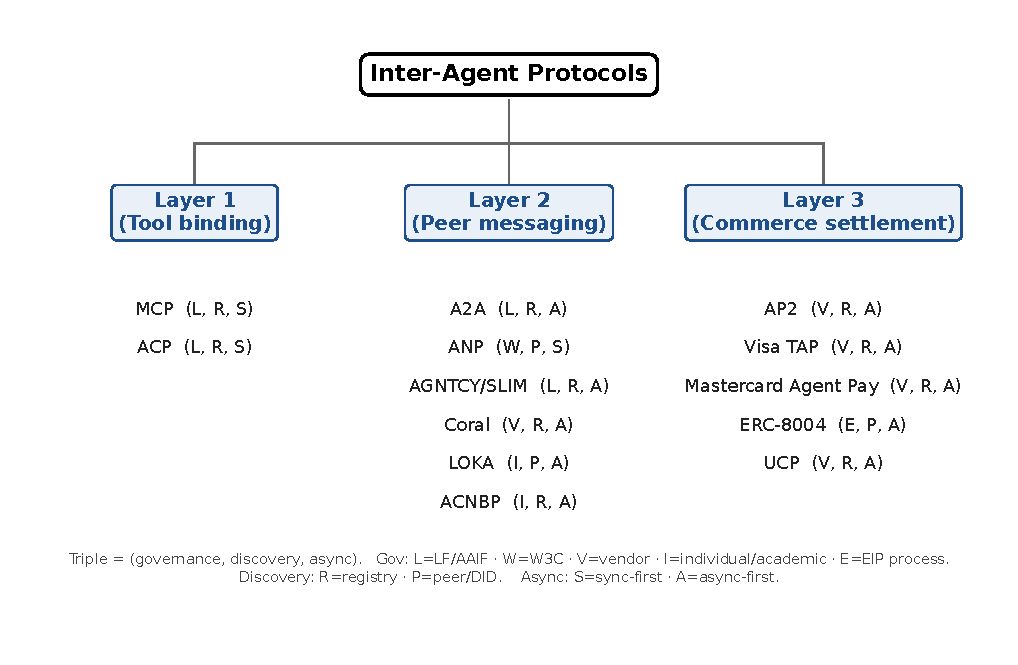
\includegraphics[width=\textwidth]{figures/fig-taxonomy.pdf}
  \caption{Three-layer taxonomy of the thirteen protocols
  surveyed. Layer assignment is by the coordination
  question the protocol answers, not by technology choice.
  Each leaf carries the orthogonal-axes triple
  (governance, discovery, async) introduced earlier in
  this section.}
  \label{fig:taxonomy}
\end{figure*}

\subsection{Why MCP and A2A are complementary, not competitive}
\label{sec:taxonomy:complementary}

The most-discussed apparent rivalry in the contemporary
literature is between MCP and A2A. Vendors and commentators
have repeatedly framed the choice as a binary: \emph{do we
ship MCP or A2A?} The framing is a category error, and
clarifying it is the single most useful corrective the
taxonomy contributes.

MCP is a tool-binding protocol. Its design answers the
question \emph{how does an agent invoke external
capabilities?} The asymmetric client-server shape, the
JSON-Schema input contracts, the streaming-result
extension, and the OAuth-2.1 transport security model are
all coherent answers to that question. MCP does not
specify how two long-lived agents coordinate; it does not
need to.

A2A is a peer-messaging protocol. Its design answers the
question \emph{how do two agents coordinate over a
long-lived task?} The Task lifecycle, the Parts and
Artifacts content model, the AgentCard discovery
convention, and the push-notification async pattern are
all coherent answers to that question. A2A does not
specify how a single agent extends itself with external
tools; it does not need to.

A production multi-agent deployment with both kinds of
coordination will typically run MCP \emph{inside} each
A2A agent, with MCP servers providing the agent's
tool-binding layer and A2A providing the inter-agent
coordination layer above. The two protocols are designed
to compose. Several emerging frameworks, including
Coral~\cite{spec_coral}, explicitly assume this
composition: Coral's tool integration is MCP-mediated
while its inter-agent threads are peer-messaging at a
different layer.

The same composition extends to the commerce-settlement
layer: where an A2A agent acts on behalf of a human
principal in a transaction, AP2 or Visa TAP carries the
intent-mandate-receipt chain alongside the A2A task,
without either protocol needing to absorb the other's
concerns. The three-layer taxonomy is, in this sense, not
merely descriptive; it is the assumption that lets the
protocols of the period \emph{compose} rather than
\emph{conflict}.

\section{The Evaluation Rubric}
\label{sec:rubric}

The rubric is the central contribution of this survey
(Contribution C1, \S\ref{sec:intro:contributions}) and the
primary instrument by which subsequent sections compare the
eight protocols of the tool-binding and peer-messaging
layers. It comprises ten evaluation axes spanning
discovery, identity, authorization, transport, task
semantics, async behaviour, multi-modal handling, security,
semantic interoperability, and governance. Seven of the ten
axes (Axes 1, 2, 3, 5, 6, 7, and 9) use anchored ordinal
scoring on a 0 to 3 scale; one (Axis 4, Transport) is a
structured tuple; one (Axis 8, Security) is a count over a
fixed twelve-item threat catalogue; one (Axis 10,
Governance/License/Observability) is a composite triple
combining a categorical governance class, a license
identifier, and a 0 to 3 observability score. The asymmetry
between ordinal, tuple, count, and composite forms is
deliberate (\S\ref{sec:rubric:goals}): forcing every axis
into the same numerical form would impose a false precision
on dimensions where it is not warranted.

\subsection{Design goals}
\label{sec:rubric:goals}

Four design constraints shaped the rubric.

\paragraph{D1: Uniform applicability across heterogeneous
protocols.} The rubric must apply consistently to a
tool-binding protocol (MCP) and a peer-messaging protocol
(A2A) and a commerce-settlement protocol (AP2) without
re-defining axes per layer. Where an axis is structurally
inapplicable to a given protocol (e.g., multi-modal content
handling for a settlement-attestation protocol), the score
records \emph{not applicable} rather than artificially low.

\paragraph{D2: Anchored descriptors, not free-form numerals.}
Each ordinal level (0, 1, 2, 3) for an ordinal axis carries an
explicitly named anchor descriptor in this section. A score
of 2 for Axis 1 (Discovery) on protocol P means \emph{P
exhibits the level-2 descriptor}, not \emph{P is somewhere
between protocols Q and R}. Anchoring is the only way to
prevent the score from collapsing into the surveyor's
subjective ordering, which is the principal weakness of the
qualitative comparison tables in the prior
surveys~\cite{yang2025survey, ehtesham2025interop}.

\paragraph{D3: Refusal to manufacture composite scores.}
The rubric is presented as a multi-dimensional matrix
(Table~\ref{tab:rubric-matrix}), a heatmap
(Figure~\ref{fig:heatmap}), and per-protocol radar charts
(Figure~\ref{fig:radar}). No single composite score is
computed. Composite scores would invite ranking, ranking
would invite optimization-by-vendor, and the resulting
benchmark-gaming dynamic has repeatedly distorted
comparable agent-evaluation work. Per-axis scores remain
defensible; their sum or weighted average does not.

\paragraph{D4: Re-runnable figures from a machine-readable
source of truth.} Every score in Table~\ref{tab:rubric-matrix},
every cell in Figure~\ref{fig:heatmap}, and every spoke in
Figure~\ref{fig:radar} is regenerated from
\texttt{data/protocol-scores.yaml} by the scripts in the
companion repository (Contribution C4,
\S\ref{sec:intro:contributions}). A future reader who
disputes a score can fork the YAML, change the cell, and
re-run the figure generation; the survey's claims are
re-runnable rather than only re-readable. This goal
concerns the path from a score to a figure. It says nothing
about whether a second rater would assign the same score,
which is a separate property that
\S\ref{sec:rubric:calibration} addresses on its own terms.

\subsection{The ten axes}
\label{sec:rubric:axes}

\subsubsection{Axis 1: Discovery and Registry Model}
\label{sec:rubric:axis1}

This axis evaluates how an agent locates another agent and
acquires the metadata necessary to interoperate. It captures
both the discovery primitive (well-known endpoint, DNS-like
directory, DID resolver, content-addressed registry) and the
strength of the verifiability guarantees the discovery layer
provides.

\begin{description}
  \item[Score 0: Out-of-band only.] No protocol-level
    discovery primitive. Agents must be configured with
    endpoints through external means (configuration files,
    environment variables, hand-edited registries). MCP in
    its stdio-only configuration sits near this baseline.
  \item[Score 1: Well-known endpoint or
    config-mediated.] A documented convention by which a
    client can probe a host for a service descriptor
    (e.g., A2A's \texttt{/.well-known/agent-card.json}~\cite{spec_a2a}).
    Centralized; trust delegated to the hosting authority.
  \item[Score 2: Federated directory with structured
    descriptors.] A directory-like service (registry,
    federated catalogue, on-chain index) returning typed
    descriptors. ACNBP's Agent Name Service~\cite{spec_acnbp}
    and Coral's MCP-mediated \texttt{list\_agents} flow~\cite{spec_coral}
    sit here.
  \item[Score 3: Decentralized verifiable resolution.]
    Discovery returns cryptographically-verifiable
    descriptors resolvable independently of any single
    authority. Typified by DID-resolver-based discovery in
    ANP~\cite{spec_anp} and LOKA's Semantic Discovery
    Fabric~\cite{spec_loka}.
\end{description}

Evidence supporting an Axis 1 score must point to a specific
section of the protocol specification that describes the
discovery primitive, the descriptor schema, and the
verification mechanism (or its explicit absence).

\subsubsection{Axis 2: Identity and Authentication}
\label{sec:rubric:axis2}

This axis evaluates the mechanism by which an agent
establishes who it is to its counterparties and how that
claim can be verified. Modern inter-agent protocols span a
range from process-bound identity (the stdio-invoked
process inherits its parent's trust) through bearer-token
schemes (OAuth~\cite{rfc6749}) to fully decentralized
identifiers (DIDs~\cite{w3c_did_core}) with verifiable
credentials~\cite{w3c_vc_data_model}. The anchors below name
those three standards, so a reader can check a score against
the normative text rather than against our paraphrase.

\begin{description}
  \item[Score 0: Process trust or unspecified.] No
    protocol-level identity mechanism. Trust derives from
    process-control (the parent invoked the child) or is
    deferred to the deployment environment.
  \item[Score 1: Bearer tokens (OAuth 2.x or
    equivalent).] Identity carried by a token issued by a
    third-party authority. A2A in its standard
    configuration~\cite{spec_a2a}, MCP over HTTP+OAuth
    2.1~\cite{spec_mcp}, and ACP all sit at level 1.
  \item[Score 2: Bearer tokens hardened with mTLS or
    signed envelopes.] Bearer credentials augmented with
    cryptographic transport binding or message-level
    signatures resistant to bearer-token theft. ACNBP's
    X.509 + OCSP + ECC-signed envelope
    structure~\cite{spec_acnbp} sits at level 2.
  \item[Score 3: Decentralized identifiers with
    verifiable credentials.] Identity established by a
    cryptographic identifier (typically a
    DID~\cite{w3c_did_core}) whose
    associated keys can sign arbitrary
    challenge-response exchanges, paired with W3C
    Verifiable Credentials~\cite{w3c_vc_data_model} for
    attribute assertions.
    ANP~\cite{spec_anp}, LOKA~\cite{spec_loka}, and Coral
    (DIDs plus Solana wallets) sit at level 3.
\end{description}

The prior survey by Kong et al.~\cite{kong2025communication}
treats identity primarily through the security lens; we
score it separately here to distinguish the
\emph{identity-modeling} contribution of a specification
from its \emph{threat-mitigation coverage} (Axis 8).

\subsubsection{Axis 3: Authorization and Delegation Model}
\label{sec:rubric:axis3}

This axis evaluates how a protocol expresses what an
authenticated agent is allowed to do, and how authorization
propagates across delegation chains (agent A asks agent B
to do X on behalf of principal P). The contemporary
literature treats this as the most under-developed area of
the contemporary protocols~\cite{authz_propagation,
agentic_jwt}; the rubric captures the gap explicitly.

\begin{description}
  \item[Score 0: Unspecified.] No protocol-level
    authorization primitives. Authorization, if any, is
    enforced at the application layer.
  \item[Score 1: Scope tokens or token forwarding.]
    OAuth-style scopes carried in bearer tokens; or the
    token-forwarding pattern in which agent A passes its
    own access token onward to agent B. Carries no
    cryptographic delegation chain; the receiver cannot
    distinguish ``the principal authorized this agent''
    from ``a previous agent in the chain authorized this
    onward call.'' A2A sits at level 1 because it
    standardises no delegation credential: \S7.5 of the
    specification makes authorization logic
    implementation-specific and leaves the choice of
    delegation mechanism to the surrounding identity
    architecture~\cite{spec_a2a}. Deployments then adopt
    token forwarding, which is where the security
    literature observes it~\cite{authz_propagation,
    agentic_jwt}. MCP's OAuth scopes also sit at level 1.
    The level is an omission at the specification layer,
    not a pattern either specification prescribes.
  \item[Score 2: Verifiable-credential-scoped
    capabilities or structured delegation tokens.]
    Authorization expressed as a signed capability with
    explicit scope, audience, and time bounds, but
    without a fully standardized chain-of-custody format.
    ANP's VC-scoped capabilities~\cite{spec_anp}, LOKA's
    smart-contract lifecycle policies~\cite{spec_loka}, and
    ACNBP's Capability Binding ceremony~\cite{spec_acnbp}
    sit at level 2. Each binds authority cryptographically
    between two named parties. None specifies how that
    authority travels further.
  \item[Score 3: Cryptographically-bound capability
    chains.] Multi-step delegation expressed as a
    composable chain of signed capabilities (or a
    capability-binding ceremony) in which each
    intermediate agent's authorization is independently
    verifiable. The second clause is the demanding one: a
    downstream agent must be able to check an upstream
    grant it did not witness. No peer-messaging protocol in
    the scored set reaches this level
    (\S\ref{sec:comparison:derivation}). The
    commerce-settlement protocols
    (\S\ref{sec:industry-protocols}) do reach it, by
    construction, through their intent-mandate-receipt
    envelope, and the agentic-JWT
    proposal~\cite{agentic_jwt} is the leading candidate
    for porting the level to the peer-messaging layer.
\end{description}

\subsubsection{Axis 4: Transport and Wire Format}
\label{sec:rubric:axis4}

The transport axis is recorded as a structured tuple rather
than an ordinal score. A single number cannot capture the
joint specification of transport bindings, serialization
format, streaming mechanism, and async-delivery primitive.
The tuple has the following fields, each populated from the
protocol specification:

\begin{itemize}
  \item \texttt{transports}: ordered list of binding
    technologies (e.g., \texttt{HTTPS/JSON-RPC 2.0},
    \texttt{stdio}, \texttt{HTTP+SSE}, \texttt{streamable-HTTP},
    \texttt{gRPC}, \texttt{REST}, \texttt{WebSocket}).
  \item \texttt{serialization}: payload encoding
    (e.g., \texttt{JSON}, \texttt{JSON-LD}, \texttt{multipart},
    \texttt{Protocol Buffers}).
  \item \texttt{streaming}: in-protocol streaming mechanism
    if any (\texttt{SSE}, \texttt{chunked HTTP},
    \texttt{WebSocket frames}, \texttt{none}).
  \item \texttt{async}: long-running-operation delivery
    primitive (\texttt{push notifications},
    \texttt{polling}, \texttt{webhooks},
    \texttt{durable resumable tasks}, \texttt{intent-centric
    peer-to-peer}).
\end{itemize}

The tuple is reported alongside the ordinal axes in
Table~\ref{tab:rubric-matrix}; it is not aggregated. Its
purpose is to support the comparison of like-with-like
transport choices (e.g., MCP's \texttt{stdio} versus
\texttt{streamable-HTTP} variants) without collapsing
distinct engineering trade-offs into a single
``transport richness'' score.

\subsubsection{Axis 5: Task and Conversation Model}
\label{sec:rubric:axis5}

This axis evaluates whether the protocol treats
multi-message interactions as first-class objects with a
defined lifecycle, or treats them as ad-hoc sequences of
independent request-response exchanges.

\begin{description}
  \item[Score 0: Stateless request/response only.] No
    notion of a multi-message interaction; each message
    stands alone. The receiver carries no protocol-level
    state from one call to the next.
  \item[Score 1: Session-scoped but no task object.]
    A session identifier groups related messages but the
    protocol defines no terminal status or artifact
    aggregation. MCP in its standard request/response
    configuration sits near level 1.
  \item[Score 2: Persistent multi-participant
    interaction.] A stateful conversation object groups
    messages, supports multiple participants, but lacks a
    full lifecycle state machine with sub-task
    delegation. Coral's persistent threads~\cite{spec_coral}
    sit at level 2.
  \item[Score 3: Full task object with lifecycle,
    artifacts, and sub-task delegation.] Tasks are
    first-class with defined lifecycle states (e.g.,
    \emph{submitted}, \emph{working}, \emph{input-required},
    \emph{completed}, \emph{failed}, \emph{canceled}), an
    artifact aggregation model, and primitives for
    delegating to a sub-task. A2A~\cite{spec_a2a} and
    ACNBP's 10-step bound-execution
    machine~\cite{spec_acnbp} sit at level 3.
\end{description}

\subsubsection{Axis 6: Async and Long-Running Operations}
\label{sec:rubric:axis6}

This axis evaluates the protocol's support for operations
whose duration exceeds the lifetime of a single connection
or even the lifetime of either communicating agent. It is
distinct from Axis 5 (which evaluates whether tasks exist
as first-class objects) because a protocol can offer rich
task semantics over short-lived connections and still
struggle with multi-hour operations.

\begin{description}
  \item[Score 0: No async primitive.] All operations
    complete within a single request/response cycle or
    fail.
  \item[Score 1: Polling-based.] Long-running
    operations are tracked by an identifier that the
    client must poll. No push delivery from server to
    client.
  \item[Score 2: Server-initiated notifications.]
    The server can push notifications or events back to
    the client via a long-lived stream (SSE,
    WebSockets) but the conversation is bound to the
    open connection.
  \item[Score 3: Durable resumable tasks.] Operations
    survive connection loss; on reconnect, the client
    resumes the task by its identifier and receives a
    complete or partial result and any backfilled
    events. A2A's push notifications combined with
    durable resumable tasks~\cite{spec_a2a} sits at
    level 3; LOKA's checkpoint-and-recovery
    machinery~\cite{spec_loka} is conceptually at level
    3 though implementation-incomplete.
\end{description}

\subsubsection{Axis 7: Multi-Modal Content Handling}
\label{sec:rubric:axis7}

This axis evaluates the protocol's vocabulary for content
beyond plain text. Multi-modal handling has emerged as a
first-class concern only in the 2024 to 2026 wave; older
ACLs and most service-oriented stacks treated content as
opaque payload with at most a MIME type.

\begin{description}
  \item[Score 0: Plain text payload only.] Messages
    carry text; binary or structured content is the
    caller's problem.
  \item[Score 1: Text plus referenced attachments.]
    Messages can reference external content via URLs or
    file handles but do not specify a typed inline part
    model.
  \item[Score 2: Typed content blocks.] A small set of
    typed parts (text, image, structured data, file)
    that can be composed within a single message. MCP's
    typed content blocks~\cite{spec_mcp} sit at level 2.
  \item[Score 3: Typed parts with inline-or-reference
    duality and content negotiation.] A complete part
    model in which each part declares its MIME type, its
    transmission mode (inline or by reference), and can
    participate in capability negotiation between
    sender and receiver. A2A's TextPart/FilePart/DataPart
    model~\cite{spec_a2a} sits at level 3.
\end{description}

\subsubsection{Axis 8: Security Threat Surface}
\label{sec:rubric:axis8}

This axis is the only count-based axis in the rubric. We
maintain a fixed twelve-item catalogue of inter-agent
protocol threats, drawn from synthesis of the security
literature~\cite{kong2025communication, a2asecbench,
zhan2024injecagent, agentleak, protocol_exploits,
a2a_weaknesses, threatmodel2026, did_vc_agents} and
applied uniformly:

\begin{enumerate}
  \item Authentication bypass
  \item Replay attacks
  \item Message tampering / man-in-the-middle
  \item Supply-chain attacks (registry poisoning,
    descriptor tampering)
  \item Denial-of-service
  \item Side-channel privacy leakage
  \item Decentralized-or-untrusted registry compromise
  \item Capability escalation through ambiguous
    descriptors
  \item Cross-agent privilege confusion
  \item Foundation-model layer prompt injection
  \item Audit-trail tampering / non-repudiation breach
  \item Delegation-chain forgery
\end{enumerate}

A protocol's Axis 8 score is the count $N \in [0, 12]$ of
threats explicitly addressed at the specification level
(not at the deployment level), with citations to the
specification sections that establish each mitigation. The
threat-catalogue and the per-protocol coverage details
are presented as the threat-coverage matrix
in \S\ref{sec:security}. The axis is intentionally a
\emph{count} rather than an ordinal score because the
twelve threats are heterogeneous and weighting them inside
the axis would re-introduce subjective ranking. A high
count is a necessary but not sufficient condition for
protocol security; \S\ref{sec:security} discusses the
difference.

\paragraph{Why the count alone is not enough, and what we
report beside it.}
A count treats every threat as one unit. Two protocols can
score the same and leave very different amounts of risk
behind, because one of them addressed the two cheapest
classes. Registry poisoning hands an attacker every
consumer of a poisoned descriptor; denial of service costs
availability and recovers when the load stops. Counting
them equally is the weakness a reviewer of this rubric
identified, and the count cannot answer it on its own.

Our answer is a second view, not a replacement score.
Table~\ref{tab:severity-coverage} in \S\ref{sec:security}
reports \emph{severity-weighted coverage} beside the count.
Each of the twelve classes carries a band (critical, high,
or moderate) and an integer weight (3, 2, or 1). The table
reports the addressed weight over the applicable weight,
and the unaddressed weight in the critical and high bands.

Three stated criteria assign the band. Does exploitation
let the attacker make the agent \emph{act}, rather than
only observe? Is the compromise recoverable from evidence
the protocol itself keeps? Does one exploit reach beyond
the pair of agents involved? Those criteria borrow their
structure from the OWASP AI Vulnerability Scoring
System~\cite{owasp_aivss}. That work argues that agentic
risk is dominated by loss of control over agent actions,
not over data alone. We do not report an AIVSS score.
AIVSS scores a concrete vulnerability in a concrete
deployment. We band a threat class against a
specification, which carries no exploit-maturity signal
and no environment.

This is deliberately consistent with D3 rather than an
exception to it. The severity view is a second reported
column, not a collapsed protocol quality score. Its
weights are published in the companion repository, so a
reader who disputes a band can change the weight and
regenerate the table. What D3 refuses is a single number
standing in for ten axes. Reporting a count and a
severity-weighted view of the same axis, with the weights
exposed, is the opposite move. It makes the weighting
argument explicit instead of hiding it inside an ordinal.

\subsubsection{Axis 9: Semantic Interoperability}
\label{sec:rubric:axis9}

This axis evaluates the protocol's mechanism for ensuring
that the meaning of an exchanged capability description,
intent, or parameter is interpretable by parties that did
not jointly author the descriptor. Section~\ref{sec:semantic}
treats this as a distinct concern from message passing.

\begin{description}
  \item[Score 0: Free-text only.] Descriptors are
    natural-language strings with no machine-tractable
    semantics.
  \item[Score 1: Structured schemas with free-text
    descriptions.] Typed input/output schemas (e.g.,
    JSON Schema) for parameters, but the human-meaningful
    description of what a capability does remains free
    text. MCP, A2A, and Coral all sit at level 1.
  \item[Score 2: Ontology-base or semantic-discovery
    indexing.] An ontology, vocabulary, or
    semantic-indexing mechanism that constrains
    capability descriptors to a shared term space.
    ANP's JSON-LD vocabulary with Agent Description
    Protocol~\cite{spec_anp} sits at level 2 at the
    cutoff; \S\ref{sec:semantic:ontology} records a
    post-cutoff narrowing of that commitment.
  \item[Score 3: Full capability ontology with
    semantic matching.] A specified ontology of
    capabilities and intents, supported by a matching
    mechanism (semantic-similarity search or
    logic-based reasoning) that produces verifiable
    semantic alignments. LOKA's Polyglot Intent Engine
    and capability ontologies~\cite{spec_loka} are
    aspirational level 3; no surveyed protocol
    \emph{ships} level 3 as of 2026-Q1.
\end{description}

The recurring gap between level 1 (where the LLM-era
protocols cluster) and level 3 (where FIPA-SL and full
ontology commitments once aimed) is the principal subject
of \S\ref{sec:semantic} and of the open-problems
agenda (\S\ref{sec:openproblems}).

\subsubsection{Axis 10: Governance, License, and Observability}
\label{sec:rubric:axis10}

The final axis is a composite triple recording three
institutional and operational characteristics that the
prior surveys treat only in passing:

\begin{itemize}
  \item \textbf{Governance}: the legal entity or
    community that holds standardization authority over
    the specification. We record the entity by name
    (e.g., \emph{Linux Foundation}, \emph{Linux
    Foundation AAIF}~\cite{lf_aaif},
    \emph{community / W3C-aligned}~\cite{w3c_agent_protocol_cg},
    \emph{individual authors}, \emph{Coral Protocol team},
    \emph{academic authors}).
  \item \textbf{License}: the license under which the
    specification (and any reference implementation) is
    distributed (e.g., Apache~2.0, MIT-equivalent,
    CC-BY-4.0, CC-BY-NC-SA~4.0).
  \item \textbf{Observability}: an ordinal 0 to 3 score on
    the protocol's specification of audit, tracing, and
    monitoring primitives (level 0 = unspecified;
    level 1 = logging hooks emerging; level 2 = trace
    fields specified, no audit primitive; level 3 =
    immutable audit trail and observability primitives
    specified).
\end{itemize}

The triple of steward, license, and observability score
is reported as a single composite cell in
Table~\ref{tab:rubric-matrix} and is unpacked into its
component analyses in \S\ref{sec:governance}.

\subsection{Scoring methodology}
\label{sec:rubric:method}

Scores are derived from a structured reading of each
protocol specification at its declared surveyed version
(2026-Q1 cutoff). The procedure for each
\emph{(protocol, axis)} pair is:

\begin{enumerate}
  \item Identify the specification section(s) relevant to
    the axis.
  \item Map the section's behaviour to the anchored
    descriptors of the axis.
  \item Record the resulting score, a one-sentence
    evidence summary, and the citation(s) supporting the
    evidence.
  \item Where a protocol specification is ambiguous, the
    score reflects what the specification \emph{requires},
    not what reference implementations \emph{do}. A
    facility provided only by a non-canonical
    implementation is recorded in evidence but does not
    elevate the score.
\end{enumerate}

Scores are stored as \texttt{data/protocol-scores.yaml} in
the companion repository (Contribution C4) and regenerate
Table~\ref{tab:rubric-matrix} and Figures~\ref{fig:heatmap}
and~\ref{fig:radar} mechanically. Anyone more interested
in the basis of a given score should consult the cited
specification section first and the YAML entry second; the
entry will name the specific evidence the score rests on.

\paragraph{What the rubric does not produce.} The rubric
does not produce a single composite ``protocol quality''
score. It does not produce a ranking. It does not produce
a recommendation: the appropriate choice of protocol
depends on deployment-specific axes that lie outside the
specification (operational maturity, ecosystem support,
internal toolchain compatibility) and that no
spec-reading exercise can determine. The rubric produces
a \emph{normalized comparison surface}; the user of the
comparison brings the application-specific weighting.

\subsection{Calibration, adjudication, and rater agreement}
\label{sec:rubric:calibration}

The procedure above says how a score is derived. It does
not say how two people applying it reach the same number.
An anchored rubric that different readers score differently
is not yet a normalized comparison surface. This subsection
closes that gap in three parts. First, the calibration
rules a rater applies at a contested boundary. Second, two
worked examples of those rules deciding a real case. Third,
an honest statement of what agreement evidence this survey
does and does not carry.

\paragraph{Four calibration rules.}
Every contested call in this survey was settled by the same
four rules, applied in order.

\begin{enumerate}
  \item \textbf{Normative text beats prose.} A mechanism
    counts at the level the specification \emph{requires}
    it. Language in an overview, a rationale, or a
    non-normative appendix supports at most the level
    below.
  \item \textbf{Spec beats implementation.} A facility that
    only a reference implementation provides is recorded in
    the evidence field and does not raise the score. This
    is rule 4 of \S\ref{sec:rubric:method}, restated here
    because it decides more boundary cases than any other.
  \item \textbf{The lower anchor wins a tie.} If a rater
    can argue the case at either of two adjacent levels,
    the score is the lower one. The asymmetry is
    deliberate. It makes the rubric under-credit rather
    than over-credit, which is the safer error for a
    reader deciding whether to depend on a protocol.
  \item \textbf{Absence of a primitive is not
    inapplicability.} \emph{Not applicable} is reserved for
    a threat or facility that is structurally outside the
    protocol's scope, not for one the protocol simply
    omits. MCP has no AgentCard, so the AgentCard
    supply-chain class is \texttt{na} for MCP. ACP has an
    unsigned manifest that plays the same role, so the same
    class is \texttt{not\_addressed} for ACP, not
    \texttt{na}.
\end{enumerate}

\paragraph{Worked example 1: ACP, Axis 2 and the
impersonation cell.}
An early pass scored ACP's identity layer as
OAuth-scope-based, on the strength of the specification's
prose about deployment behind an authenticating reverse
proxy. Re-reading the OpenAPI document showed it declares
no \texttt{securitySchemes} at all. Rule 1 settles it: the
prose is not normative, the machine-readable contract is,
and a mechanism the contract does not declare cannot be
scored. Rule 2 blocks the fallback argument that ACP
deployments do authenticate in practice. The impersonation
cell moved to \texttt{not\_addressed} and ACP's Axis 8
count moved to 1. A second rater who applies rules 1 and 2
to the same OpenAPI document reaches the same cell. The
question the rules ask has a yes-or-no answer in the
document rather than a judgement.

\paragraph{Worked example 2: AGNTCY, the audit-log
tampering cell.}
AGNTCY persists scan reports as OCI referrers and emits
OpenTelemetry traces. Both are real, specified, and
relevant to audit. Neither is a tamper-evident log: nothing
in the specification prevents a party with write access
from rewriting the record. The candidate scores are
\texttt{addressed} (an audit mechanism is specified) and
\texttt{partial} (the mechanism is specified but the
integrity property is not). Rule 3 decides it as
\texttt{partial}, and the cell's evidence field records the
reason in the same words. The same rule applied to Coral's
blockchain-anchored trail returns \texttt{addressed},
because there the integrity property is the mechanism. The
contrast is what makes the boundary reproducible: the rater
is not asked whether the audit story is good, but whether
the specification names an integrity guarantee.

\paragraph{Adjudication when the rules do not settle it.}
Two cases survive the four rules. The first is a
specification whose text is genuinely ambiguous about what
it requires. Here we wrote to the specification's authors,
and where they answered, the answer is recorded as evidence
and the score follows it. Two scores in this survey moved
that way. ACNBP's Axis 3 dropped from 3 to 2 after a lead
author confirmed that the Capability Binding ceremony is a
two-party protocol. Multi-agent delegation is outside its
scope (\S\ref{sec:security:authz}). ANP's task-model scope
was recorded as deliberate rather than underspecified after
the same kind of exchange. The second
case is a specification that changed after we scored it.
There the cutoff governs: the score stands at the surveyed
version, and the drift is recorded rather than silently
absorbed (\S\ref{sec:rubric:limits}).

\paragraph{What agreement evidence we have, and what we do
not.}
We state this plainly, because the rubric's value depends
on it. This survey does not report an inter-rater
reliability statistic. No second rater independently scored
the full matrix. We therefore have no Cohen's $\kappa$ and
no agreement percentage to offer, and we decline to compute
one from a process that would not support it.

What we have instead is an auditable change history. Every
score lives in \texttt{protocol-scores.yaml} with an
evidence string. Every change to a score is a commit with a
stated reason. The counting rule for Axis 8 is enforced by
a check in the companion repository, which fails the build
when a count and the threat matrix disagree. That check
exists because they did disagree: four protocols carried
counts that had absorbed \texttt{partial} cells, which the
axis definition excludes, and nothing caught it because
nothing was checking. Coverage of the manuscript prose was
added to the same check for the same reason.

An auditable trail is weaker evidence than two independent
raters, and we do not present it as equivalent. It supports
a narrower claim: that each score is traceable to a
specification passage a disputing reader can check, and
that no score has moved without a recorded reason. The
axes most exposed by the gap are the two most
judgement-heavy ones: semantic interoperability (Axis 9)
and the observability component of Axis 10. In both, the
anchors describe a degree of specification rather than the
presence of a named mechanism. A two-rater pass over them
is the highest-value item in the rubric's own future work,
and \S\ref{sec:openproblems:benchmarking} lists it there.

\subsection{Limitations of the rubric}
\label{sec:rubric:limits}

Four limitations of the rubric require explicit
acknowledgement.

\paragraph{The rubric covers eight of the thirteen surveyed
protocols.} Every score in this survey is a score of one of
the eight tool-binding or peer-messaging protocols. The five
commerce-settlement protocols (AP2, Visa TAP, Mastercard
Agent Pay, ERC-8004, UCP) are surveyed and compared, in
\S\ref{sec:emerging:commerce} and
Table~\ref{tab:commerce-stack}, but they are not rubric
scored. The reason is that six of the ten axes have no
referent in a settlement envelope: it has no task state
machine, no async resumption model, no multi-modal content
negotiation, and its discovery and transport are those of
whichever peer-messaging protocol carries it. Scoring them
anyway would produce rows of \texttt{n/a} and a set of
figures whose averages moved for reasons of scope rather
than of substance.

UCP is the one member of the layer where that reason is
weaker. It specifies discovery, authentication,
authorization, and four transport bindings
(\S\ref{sec:emerging:commerce}), so four axes would return a
defensible score. It is left unscored anyway, on two
grounds. It is a commerce-orchestration layer rather than a
peer-messaging protocol, so the axes it does answer are
answered for a different purpose. And scoring one member of
the commerce layer while four remain unscored would move the
figures' averages for reasons of scope. Its per-axis
evidence is recorded in
\texttt{data/protocol-scores.yaml} so that a later revision
widening the rubric does not start from nothing. The cost of
the choice is that the commerce layer cannot be ranked
against the other two, and a reader wanting one comparable
number across all thirteen will not find it here.

\paragraph{Subjectivity at the anchor boundaries.} The
boundary between two adjacent anchored levels is
necessarily a judgment call. We have made each boundary
description as concrete as the specification language
allows, and the four calibration rules of
\S\ref{sec:rubric:calibration} settle a contested boundary
in a stated order rather than by preference. Still, some
boundaries remain thin. A \emph{level-1} discovery primitive
is a well-known endpoint and a \emph{level-2} one is a
federated directory. Which side A2A's AgentCard convention
falls on depends on whether one reads it as a
``federation'' or as ``a
hosted convention.'' Where the boundary is contestable, we
record the reasoning in the YAML evidence field. The
residual limitation is the one
\S\ref{sec:rubric:calibration} states directly: the rules
make a boundary call reproducible in principle, and no
second rater has independently confirmed that it
reproduces.

\paragraph{Version drift across the review cycle.}
Protocols at the active 2025 to 2026 frontier are evolving
on a quarterly cadence. A score recorded against
A2A v1.0 may not hold against the version current at
publication. The companion repository's update discipline
addresses this directly: the YAML carries
\texttt{spec\_version} and \texttt{retrieved} fields per
protocol; a future reader can compute the staleness
delta. The survey itself reports scores at the declared
cutoff and does not silently update them in proof.

\paragraph{Evidence tier asymmetry.} Some protocols
(A2A, MCP) have multi-tier sourcing: an official
specification, peer-reviewed security analyses, and
production deployments. Others (ACNBP, LOKA) are at
arXiv-paper stage with no formal SDO and no large-scale
production deployment to validate the spec's
operational claims. Where the specification declares a
mechanism the rubric scores the declaration; where the
declaration depends on infrastructure that does not
yet exist (LOKA's level-3 semantic interoperability via
the Polyglot Intent Engine), the evidence field records
the gap. We are weighing scores by source tier;
\S\ref{sec:industry-protocols} and
\S\ref{sec:emerging-protocols} present the
implementation-maturity context alongside the rubric
scores.

\section{Industry-Standard Protocols}
\label{sec:industry-protocols}

This section applies the rubric of \S\ref{sec:rubric} to the
five inter-agent protocols that have either been adopted into
a formal standards body, ship with named production
deployments, or both: Google A2A, the Model Context Protocol,
IBM ACP, Cisco-led AGNTCY/SLIM, the Agent Network Protocol,
and Coral. The commerce-settlement industry-led
protocols (AP2, Visa TAP, Mastercard Agent Pay, ERC-8004, UCP) are
treated as a co-stack in \S\ref{sec:emerging:commerce} because
their design intent and rubric alignment differ from the
peer-messaging and tool-binding members of this group. Each
sub-section names the protocol's design intent, summarizes
the rubric scores, and identifies the open issues that
implementations and successor specifications must address.

\subsection{Google A2A}
\label{sec:industry:a2a}

A2A was introduced by Google in April 2025 as the canonical
peer-messaging protocol for inter-agent
coordination~\cite{spec_a2a}, and was donated to the Linux
Foundation under the AAIF umbrella in late 2025~\cite{lf_aaif}.
The protocol's defining structural choice is to treat the
\texttt{Task} as a first-class lifecycle-bearing object with
explicit submitted, working, input-required, auth-required,
completed, failed, and canceled states, and to pair the
task object
with a typed \texttt{Part} content model (TextPart,
FilePart, DataPart) that supports inline and by-reference
delivery. The discovery convention is a well-known endpoint
at \texttt{/.well-known/agent-card.json} returning a typed
AgentCard descriptor.

Rubric scores at the 2026-Q1 cutoff: Axis 1 = 1 (well-known
endpoint discovery), Axis 2 = 1 (OAuth-mediated bearer
identity), Axis 3 = 1 (advertised authentication schemes
and an in-task authorization flow, but no standardised
delegation credential), Axis 5 = 3 (full task object
with artifacts and sub-task delegation), Axis 6 = 3 (push
notifications combined with durable resumable tasks),
Axis 7 = 3 (typed parts with inline-or-reference model),
Axis 8 = 1 of 12 (transport encryption is the only
spec-level mitigation; bearer identity, push-notification
replay verification, and transport-layer DoS resistance are
partial and so do not count; injection, registry poisoning,
and delegation token theft are not addressed), Axis 9 = 1 (free-text Skill
descriptions over typed Skill objects), Axis 10
observability sub-score = 2 (SSE event stream supports
tracing; no standardized audit primitives).

The transport tuple is rich: HTTPS/JSON-RPC 2.0 as the
primary binding, optional gRPC and REST, JSON
serialization, SSE streaming, push notifications for async
delivery~\cite{spec_a2a}. The protocol composes naturally
with MCP for the tool-binding layer of each agent and with
AP2 or Visa TAP for the commerce-settlement layer
(\S\ref{sec:taxonomy:complementary}).

The specification does address authorization, and the
survey's Axis 3 score should not be read as saying
otherwise. \S7 states security requirements, the AgentCard
advertises authentication schemes, and \S7.6 defines
in-task authorization: an agent that needs further
authorization mid-task moves to the auth-required state and
delegates fulfilment of the request to its
client~\cite{spec_a2a}. What the specification leaves to
the surrounding identity architecture is authorization
policy (\S7.5 makes it implementation-specific) and the
choice of delegation mechanism. The score records that
absent credential format, not an absent security model.

The exclusion is deliberate and the specification says so
in normative language. \S7.6.4 states that A2A does not
define the scope, representation, validity, or revocation
semantics of the credential attached to the auth-required
state. It requires that the state transition alone must not
be treated as authorization for any operation, and that a
credential obtained through it must not be assumed to
authorize later messages on the same task. Meaning and scope
must come from the implementation, the credential issuer, or
an A2A extension~\cite{spec_a2a}. So A2A specifies
authorization \emph{knobs} rather than an authorization
model, and does it on purpose, so that many authorization
solutions can be plugged in above it. The survey reads that
as a scoping decision rather than an oversight. The Axis 3
score measures what a receiver can verify from the protocol
alone, which is why a deliberate exclusion and an accidental
omission land on the same level, and why
\S\ref{sec:security:authz} separates the two in prose.

The open issues against A2A at the cutoff are at the
identity and authorization layers. Eight named weaknesses
are documented in the security
literature~\cite{a2a_weaknesses}: AgentCard supply-chain
attacks, registry poisoning against the discovery convention,
delegation token theft, sensitive-data leakage through
free-text Skill descriptions, prompt-injection vectors via
DataPart payloads, replay attacks on push notifications,
side-channel privacy leakage from task lifecycle
transitions, and absent cryptographic delegation chains.
The A2ASecBench protocol-aware
evaluation~\cite{a2asecbench} catalogues several of these
empirically. Mitigations under discussion in the
Linux Foundation working group include the
ANP-style DID overlay for identity, the agentic-JWT
delegation pattern~\cite{agentic_jwt}, and the
authorization-propagation chain
proposed in~\cite{authz_propagation}; none has been
adopted into the spec as of 2026-Q1.

\subsection{Model Context Protocol (MCP)}
\label{sec:industry:mcp}

MCP is the canonical tool-binding
protocol~\cite{spec_mcp}: the asymmetric two-party
specification by which an agent (the client) invokes
external capabilities exposed as tools, resources, and
prompts. It was introduced by Anthropic in late 2024,
adopted by every major model vendor within months, and
governed under the Linux Foundation AAIF alongside
A2A~\cite{lf_aaif}.

Rubric scores: Axis 1 = 1 (server config-based discovery
with an emerging registry, mostly out-of-band), Axis 2 = 1
(OAuth 2.1 for HTTP transport, stdio relies on parent-process
trust), Axis 3 = 1 (OAuth scopes only, no agent-delegation
primitives), Axis 5 = 1 (request/response with sessions
but no protocol-level state machine; the emerging MCP Tasks
extension begins to add task semantics), Axis 6 = 2
(notifications plus emerging MCP Tasks; long-running
operations supported but not durably resumable across
connection loss), Axis 7 = 2 (typed content blocks for
text, image, and resource; structured JSON-Schema tool
input), Axis 8 = 1 of 12 (transport encryption is the
only spec-level mitigation; OAuth 2.1 identity is partial,
because the stdio transport falls back to process trust;
injection and tool poisoning remain
unaddressed at spec level~\cite{zhan2024injecagent,
protocol_exploits}), Axis 9 = 1 (JSON Schema for tool
input combined with free-text tool descriptions),
Axis 10 observability = 1 (logging hooks emerging; no
standardized audit primitives).

The transport tuple distinguishes MCP from A2A most
clearly: stdio, HTTP+SSE, and streamable-HTTP bindings; the
JSON-RPC 2.0 serialization shared with A2A; SSE or chunked
HTTP streaming; notifications and emerging MCP Tasks for
async delivery~\cite{spec_mcp}. The stdio binding is
particularly important in production: it allows a sandboxed
agent process to invoke a tool process within the same
trust boundary without the network attack surface of an
HTTP binding. The trade-off is that stdio inherits the
parent process's identity completely; the identity axis
score of 1 hides a sub-distinction between HTTP+OAuth and
stdio+process-trust that the Axis 4 tuple makes explicit.

The principal open issues at the cutoff are tool poisoning,
indirect prompt injection through tool results, and the
need for richer authorization primitives than OAuth
scopes can express. The InjecAgent
benchmark~\cite{zhan2024injecagent} establishes that
indirect injection is a measurable threat against deployed
MCP servers; the protocol does not currently specify
mitigations. The AAIF working group has begun discussing
an MCP-level authorization extension that would carry
agent-principal-delegation chains alongside OAuth scopes;
this would raise the Axis 3 score and align MCP with the
emerging chain-of-custody pattern that the
commerce-settlement layer requires.

\subsection{IBM ACP / BeeAI}
\label{sec:industry:acp}

IBM's Agent Communication Protocol (ACP), incubated under
the BeeAI project, occupies the tool-binding layer
alongside MCP but with structurally different
choices~\cite{spec_acp}. The transport is REST over HTTP,
in contrast to MCP's JSON-RPC 2.0. Serialization is JSON,
with streaming delivered as Server-Sent Events. The
positioning is stateless by design, in the sense that HTTP
is stateless: sessions are available when an agent needs
to carry state across runs.

ACP requires a status caveat that no other row in
Table~\ref{tab:rubric-matrix} needs. The specification is
\emph{complete but terminated}. The upstream repository was
archived in August 2025, and the project merged into A2A
under the Linux Foundation umbrella~\cite{spec_acp}. The
scores we report describe the specification as published,
not an effort still competing for adoption. We retain the
row because ACP is the survey's clearest evidence for
Finding~5 (\S\ref{sec:conclusion:governance}): it scores at
the top of the set on the task axis and still lost.

Rubric scores: Axis 1 = 1 (a well-known manifest at
\texttt{/.well-known/agent.yml} plus a live
\texttt{GET /agents} endpoint; registry-based discovery is
named but unspecified, and no descriptor is signed),
Axis 2 = 1 (the OpenAPI document declares no security
schemes at all; Basic, Bearer, and JWT appear only in prose,
enforced at a reverse proxy), Axis 3 = 1 (no authorization
primitive whatsoever), Axis 5 = 3 (a first-class
\texttt{Run} object with an eight-state lifecycle,
two-phase cancellation, and named artifacts), Axis 6 = 2
(asynchronous accept-and-poll, event backfill, and
distributed sessions portable across servers by URL
descriptor), Axis 7 = 2 (typed parts with inline-or-reference
duality and manifest-level content-type negotiation),
Axis 8 = 1 of 12 (transport encryption only, and that from
prose rather than specification text; the other eleven
threat classes are not addressed even partially, which is
unique in the set), Axis 9 = 1 (typed
manifest with free-text descriptions), Axis 10
observability = 2 (OpenTelemetry integration with default
exporters, plus trajectory and citation metadata carried in
the wire format).

Two features distinguish ACP, and neither is a content
format. The first is the run lifecycle. ACP defines an
\texttt{Await} mechanism by which an agent pauses execution
to request input from its client, then resumes on a
subsequent call. Combined with the eight-state machine and
named artifacts, this puts ACP at the same level as A2A on
the task axis and two levels above MCP. The second is
distributed sessions: session history and state are
referenced by URL on arbitrary resource servers, so a
session migrates between independent ACP servers by
forwarding only its descriptor, with no shared
infrastructure.

The gap between Axis 5 (level 3) and Axis 8 (1 of 12) is the
widest of any protocol we score, tied with A2A, and in ACP's
case it is deliberate rather
than accidental. ACP is HTTP-native by design, and its
answer to security is that the surrounding HTTP
infrastructure already provides one. That is a defensible
engineering position and a weak specification position. ACP
documents four multi-agent composition patterns, including
hierarchical delegation, while specifying no way for a
receiver to establish on whose authority a caller acts. It
is the sharpest instance in the survey of the
authorisation-propagation gap that Finding~3 names.

\subsection{AGNTCY / SLIM (Cisco-led)}
\label{sec:industry:agntcy}

AGNTCY is a Cisco-led collective effort hosted within the
Linux Foundation umbrella. It positions itself as a
``directory plus identity plus observability stack'' rather
than a single protocol, and that positioning has a
methodological consequence for this survey: AGNTCY is not
one specification but four. We score it across the Open
Agentic Schema Framework (OASF) for agent records, the
Agent Directory Service (ADS) for publication and
discovery, the Secure Low-latency Interactive Messaging
protocol (SLIM) for the messaging substrate, and a separate
identity specification~\cite{spec_agntcy}. ADS and SLIM are
each published as IETF Internet-Drafts. Both are individual
Independent Submissions with informational intended status,
so neither carries working-group adoption or IETF
endorsement.

OASF is the descriptor contribution, and its capability
model is stronger than free-text schemas. Records must
declare skills drawn from a published hierarchical
taxonomy, currently eighteen skill categories with nested
subcategories, alongside a parallel taxonomy of twenty
domain verticals. The framework is explicitly modelled on
OCSF, the Open Cybersecurity Schema Framework, and its
schema server is a derivative of the OCSF server. A
controlled vocabulary that constrains capability
descriptors to a shared term space is our Axis 9 level-2
anchor, so OASF scores 2. It does not reach level 3:
matching is taxonomic lookup, not semantic-similarity
search or logic-based reasoning producing verifiable
alignments.

ADS is the discovery contribution, and it is the only
industry-led effort in the survey to reach Axis 1 level 3.
Records are content-addressed by CID, so a descriptor's
identifier is a digest of its contents. Independent
directory nodes federate over a distributed hash table with
no central registry: publication announces
(CID, skills) pairs into the routing layer, and lookup
queries the skill taxonomy to retrieve matching CIDs and
their hosting nodes. Records are signed as
Cosign-compatible artifacts, with keyless OIDC, self-managed,
and KMS-backed signing flows all specified. Verifiable
names bind a signing key to a claimed domain by requiring a
JSON Web Key Set at that domain's well-known endpoint.
Discovery therefore returns cryptographically verifiable
descriptors resolvable independently of any single
authority, which is the level-3 descriptor.

SLIM is the messaging substrate, and its security
architecture is two-tier rather than transport-only. At the
network layer, HTTP/2 and HTTP/3 provide hop-by-hop TLS 1.3
encryption. HTTP/2 is the deliberate primary choice, for
compatibility with deployed load balancers, gateways, and
CDNs. Above it, Message Layer Security~\cite{rfc9420}
provides an application-layer encryption envelope
independent of the underlying TLS sessions. The consequence
is that routing nodes are zero-trust intermediaries: they
forward opaque encrypted blobs and cannot read message
content even after TLS terminates. SLIM names entities with
decentralized identifiers rather than transport
credentials. Node names are \texttt{did:key} values, client
locators compose an organization DID, namespace, service,
and client DID, and a channel is keyed to the DID of its
MLS group moderator, derived as a hash of that moderator's
public key.

Rubric scores: Axis 1 = 3 (content-addressed records over
a federated DHT with signed descriptors), Axis 2 = 2
(W3C Verifiable Credential agent badges verified through
resolver metadata, plus SPIFFE workload identity),
Axis 3 = 1 (MLS group membership plus short-lived OAuth
bearer tokens; no delegation chain), Axis 5 = 1 (sessions,
not tasks), Axis 6 = 3 (session state, group membership,
subscriptions, and pending queues survive disconnection and
node failure, with automatic reconnection and subscription
recovery), Axis 8 = 6 of 12, Axis 9 = 2 (the OASF
taxonomy), Axis 10 observability = 3, the highest of the
industry-led set, on the strength of a dedicated
observability sub-project shipping an OpenTelemetry SDK.

Two scores warrant explanation. Axis 2 sits at 2 rather
than 3 despite the use of Verifiable Credentials, because
the specification explicitly disclaims being bound by the
DID and VC standards, and its worked examples anchor agent
identifiers to enterprise identity providers whose keys
resolve from a tenant key-set endpoint. That is
issuer-anchored identity with signed credentials, not
self-sovereign control of keys. Axis 7 is 0, and the score
is an artefact of scope rather than a deficiency: a
substrate whose intermediaries cannot decrypt payloads has
no place for a content model, and MLS makes that opacity a
design guarantee. We report it as not applicable in
substance, consistent with design goal D1
(\S\ref{sec:rubric:goals}).

The AGNTCY scores make the composition argument concrete
rather than merely asserted. AGNTCY supplies discovery at
level 3, async durability at level 3, and the strongest
supply-chain posture in the survey, precisely where A2A
scores 1, 3, and partial. A2A supplies a task model and a
content model at level 3, precisely where AGNTCY scores 1
and 0. The two are complementary by construction: an
A2A-speaking agent, published as an OASF record in a
federated directory, addressed over SLIM. The open issue at
the cutoff is not whether they overlap but which stack an
adopter depends on at each layer, and the literature is not
yet mature enough to answer that.

\subsection{Agent Network Protocol (ANP)}
\label{sec:industry:anp}

ANP is the most identity-forward of the peer-messaging
protocols~\cite{spec_anp}. Its design center is the
proposition that agent identity should be decentralized,
cryptographically verifiable, and resolvable independently
of any single registry. The protocol builds on the W3C
DID and Verifiable Credentials specifications, and is the
only surveyed protocol that scores level 3 on both
Axis 1 (DID-resolver-based discovery) and Axis 2 (DIDs +
VCs for identity).

Rubric scores: Axis 1 = 3 (DID resolver plus Agent
Description Protocol), Axis 2 = 3 (DIDs and VCs as W3C
standards), Axis 3 = 2 (VC-scoped capabilities but
chain-of-custody patterns are not fully standardized),
Axis 5 = 1 (multi-turn but lightly specified at the
protocol layer), Axis 6 = 1 (polling primarily; no
push-notification standard), Axis 7 = 1 (text plus file
references), Axis 8 = 5 of 12 (identity, authentication,
integrity, audit, and non-repudiation are strong through
DIDs; operational threats are weaker, namely prompt
injection, registry poisoning, and capability escalation),
Axis 9 = 2 (JSON-LD ontology base, ADP enables semantic
discovery), Axis 10 observability = 1 (built-in
non-repudiation logs but no standardized audit dashboard).

The transport tuple is the lightest of the surveyed
peer-messaging protocols: HTTPS only, JSON-LD over JSON
serialization, no native streaming, polling for async
delivery. ANP's design accepts the latency cost of polling
in exchange for the decentralization properties that
push-notification-based architectures complicate. The
white paper~\cite{spec_anp} explicitly positions ANP for
peer-to-peer deployments where no central registry can be
assumed.

The Axis 5 and Axis 6 scores need a word on intent,
because the low numbers are a design choice rather than an
unfinished edge. The account below follows the
specification, and the ANP Community confirmed the reading
in correspondence with the authors. ANP does not treat a
task as a
protocol-level concept at all. Its first-class concepts are
Information and Interface: Information is data the agent
publishes, and Interface is an API it exposes, either
natural-language or structured. A task is then one form of
an Interface rather than an abstraction the protocol
defines. The stated reason is generality. The task concept
is useful in many settings but is not universal enough to
carry every agent interaction, so ANP keeps its primary
abstractions broader. Asynchrony follows the same rule: an
Interface defines its own asynchronous model where it needs
one, and the protocol layer defines no separate primitive.
This is the same deliberate-exclusion pattern the survey
records for A2A on Axis 3
(\S\ref{sec:security:authz}). The axis measures what the
protocol itself specifies, so a considered omission and an
unfinished one land on the same level, and the survey
separates them in prose rather than in the number.

The open issues at the cutoff are therefore operational
maturity and the consequence of that scoping choice rather
than the choice itself. ANP's strengths are at the identity
and authentication layers; the dimensions it leaves to the
Interface are precisely those on which A2A scores highest
(tasks, async, and multi-modal handling). The natural
composition pattern (ANP for identity, A2A for task
semantics) would require bridging machinery the cutoff
specifications do not yet provide.\footnote{Post-cutoff, and
recorded here because it bears on Axis 6 and Axis 9 rather
than to revise them. ANP published a 1.1 release line in
June 2026, after the 2026-Q1 cutoff, adding a released
end-to-end instant messaging suite (ANP-09) for direct and
group agent-to-agent messages with attachments and optional
end-to-end encryption~\cite{spec_anp_v11}. Its premise is
that identity plus messaging carries a large share of
collaboration without modelling each interaction as a
structured task, which is the Information-and-Interface
position above followed to its conclusion. The same release
narrows the JSON-LD commitment: the Agent Description
document (ANP-07) moved to plain JSON for readability,
while the Discovery specification (ANP-08) keeps JSON-LD
and its \texttt{@context} mechanism. The community
describes the underlying Linked Data philosophy as
retained. Section~\ref{sec:semantic:ontology} records what
this would do to the Axis 9 reading.}

\subsection{Coral Protocol}
\label{sec:industry:coral}

Coral~\cite{spec_coral} occupies the peer-messaging layer
with two distinguishing choices: persistent multi-participant
threads as the conversational primitive, and an explicit
integration with MCP for the tool-binding layer. Coral
positions itself as ``the Internet of Agents'' substrate
and supports both off-chain coordination (over standard
HTTP and SSE) and on-chain settlement (via Solana wallets
and signed team contracts) where the deployment requires
it.

Rubric scores: Axis 1 = 2 (\texttt{list\_agents} MCP tool
resolves from a server-mediated Coral Server;
blockchain-anchored but discovery is server-mediated
rather than DID-resolver), Axis 2 = 3 (each agent has a
DID and cryptographic credentials with Solana wallets as
authenticator), Axis 3 = 2 (Team Contracts as signed
multi-agent agreements, optionally on-chain; not RFC 8693,
not a fully specified delegation chain), Axis 5 = 2
(stateful persistent multi-participant threads; sub-task
delegation deferred to a future Task Management service),
Axis 6 = 2 (\texttt{wait\_for\_mentions} is an explicit
push primitive; no durable resumable spec), Axis 7 = 0
(natural-language message content with mention metadata
only; no typed parts or content negotiation), Axis 8 = 3
of 12 (DIDs and wallets for auth, on-chain immutable
audit, and thread-scoped privilege confusion are
addressed; team-contract capability escalation,
delegation token theft, and signed-transaction integrity
are partial, the last because signatures cover the payment
path rather than the message path; replay, supply-chain,
side-channel, DoS, prompt injection, and registry
poisoning not addressed), Axis 9 = 1 (Coraliser adapters
enforce uniform schemas but no formal capability
descriptor or ontology), Axis 10 observability = 2
(blockchain audit trail is mandatory for payments and
team contracts; no separate trace or metric spec).

The transport tuple is HTTP, WebSocket, and SSE
bindings; JSON via MCP serialization; SSE streaming; push
via \texttt{wait\_for\_mentions}~\cite{spec_coral}. The
choice to deliver tool semantics through MCP rather than
re-specifying them is structurally important: Coral
explicitly accepts the layer composition argument of
\S\ref{sec:taxonomy:complementary} and builds on top of
MCP rather than alongside it.

The open issues at the cutoff are content-model
poverty (Axis 7 = 0 is the lowest score in the surveyed
set), the absent task lifecycle (Axis 5 stops at level 2),
and the dependency on blockchain primitives for the
strongest security claims. Deployments that do not want
to commit to Solana settlement infrastructure inherit a
weaker version of Coral's threat model.

\section{Emerging and Specialized Protocols}
\label{sec:emerging-protocols}

This section applies the rubric to the protocols whose
2026-Q1 maturity is at the academic-paper, arXiv-draft, or
EIP-draft stage rather than at the production-deployment
stage of the protocols in \S\ref{sec:industry-protocols}.
The lower deployment maturity does not imply lower
significance: ACNBP's capability-binding ceremony and LOKA's
verifiable-credential framework address gaps that the
industry-standard protocols have left open, and the five
commerce-settlement protocols introduce an architectural
layer that the prior surveys did not cover.

\subsection{LOKA}
\label{sec:emerging:loka}

The LOKA Protocol~\cite{spec_loka} is the most
ambitious peer-messaging proposal of the surveyed set in
the sense that it commits, at the specification level, to
the strongest version of every axis where the
industry-standard protocols make pragmatic concessions.
LOKA proposes a Semantic Discovery Fabric (Axis 1
score = 3), DIDs with Ed25519 keys and post-quantum
Dilithium upgrades (Axis 2 score = 3), VCs as scoped
capability attestations combined with smart-contract
lifecycle policies (Axis 3 score = 2), an
intent-centric peer-to-peer async model with continuous
checkpointing and recovery (Axis 6 score = 3), a Polyglot
Intent Engine targeting FIPA-ACL, A2A, and Open Voice
interoperability (Axis 9 score = 3 aspirationally), and
immutable blockchain-backed audit trails with real-time
ethical auditing (Axis 10 observability = 3).

The authors themselves note in a footnote that LOKA is a
conceptual research framework; the cited specification
declares mechanisms but does not yet ship reference
implementations of most of them. The Axis 4 transport
tuple records this: \texttt{transports = unspecified},
\texttt{streaming = unspecified}, \texttt{async =
intent-centric peer-to-peer (unspecified)}~\cite{spec_loka}.
The strength of LOKA in the rubric matrix is therefore
that it occupies the upper-right corner on most axes; the
weakness is that the implementation-maturity context that
\S\ref{sec:rubric:limits} flags applies in full. A
reader weighting the survey by source tier should treat
LOKA's scores as aspirational claims about a possible
future protocol rather than as verifiable claims about a
deployed one.

The Axis 8 score of 6 of 12 reflects an explicit
threat-modeling pass in the LOKA paper that addresses
DID-and-Dilithium authentication, timestamp-and-signed-intent
replay, blockchain audit, post-quantum MITM,
decentralized-SSI registry, and Contextual Ethics privilege
confusion. Four further classes are treated but not settled,
so they score partial and do not enter the count: the DECP
prompt-injection filter, VC-and-contract capability scoping,
delegation token binding, and the privacy side of Contextual
Ethics. Supply-chain attacks and DoS are unaddressed.

\subsection{Agent Capability Negotiation and Binding Protocol (ACNBP)}
\label{sec:emerging:acnbp}

ACNBP~\cite{spec_acnbp} is the most security-rigorous of the
emerging protocols in the rubric matrix. Its Axis 8 score of
10 of 12 is the highest of any protocol surveyed, the
direct consequence of an explicit MAESTRO 7-layer threat
analysis in the specification that addresses zero-knowledge
proof capability attestations, signature plus HMAC
integrity, rate-limit-and-proof-of-work DoS mitigation,
nonce-and-timestamp-and-sequence replay defense, a
\texttt{protocolExtension} whitelist for supply-chain
attacks, X.509 with OCSP against agent impersonation, the
Capability Binding ceremony against delegation-token theft,
signed Agent Network Resource Identifiers with BFT for
registry integrity, foundation-model-layer prompt injection
mitigation, and cryptographically protected audit logs. The
two classes that score partial, and so do not enter the
count, are side-channel privacy through ring signatures and
cross-agent privilege confusion through agent quarantine.

The protocol's structural contribution is the ten-step
capability negotiation and binding flow. Two agents that
have located each other through the ANS directory
exchange capability descriptors, run a semantic
consistency check, propose binding terms, negotiate
modifications, and conclude with a mutually-signed
Capability Binding (the central primitive defined in
Definition 10 of the specification). The bound capability
is then executable as an artifact-producing operation
whose execution produces a cryptographically attested
receipt. The Axis 5 score of 3 (10-step state machine
with Protocol State as a first-class object) follows
directly from this structure.

Authorization is where that structure stops, and the
boundary is worth stating precisely because it is easy to
misread. Definition 10 binds two parties: a requester and
a provider, with capabilities, terms, and mutual
signatures. That is one hop, and it is bound more
rigorously than any other peer-messaging specification
binds one hop. It is not a chain. The ACNBP text never
uses the words delegation, authorization, on behalf,
principal, or sub-agent, and the nearest multi-agent
construct, the Multi-Agent Orchestration paragraph of
\S IV.C, describes capability composition rather than
transitive authority. The Axis 3 level-3 anchor
(\S\ref{sec:rubric:axis3}) asks whether a downstream
agent can independently verify an intermediate agent's
grant. Nothing in ACNBP answers that, so the Axis 3
score is 2, which is the anchor for a structured
capability with explicit scope and no standardized
chain-of-custody format. A lead author
confirmed the reading in correspondence: ACNBP is a
two-party protocol for service negotiation and binding,
and multi-agent delegation is outside its scope. The
consequence for the field is in
\S\ref{sec:comparison:derivation}, and it is the
strongest form of the survey's central finding: no
scored protocol reaches level 3, including the most
security-rigorous one.

Identity is the one axis where ACNBP's own text is
narrower than its authors' work. The specification
authenticates agents with X.509 certificates, OCSP
revocation, and signed envelopes, which is Axis 2 level 2,
and it never mentions decentralized identifiers or
verifiable credentials. The same authors do treat
decentralized identity, in a companion framework built on
DIDs and verifiable credentials with a naming service and
zero-knowledge attribute
disclosure~\cite{huang_zerotrust_identity}. ACNBP cites
that framework as related work and does not require it, so
the Axis 2 score records what ACNBP itself specifies. The
survey scores specifications, not the composition a reader
could assemble from a research group's output
(\S\ref{sec:rubric:method}). Were the companion framework
folded in normatively, ACNBP would be a candidate for
Axis 2 level 3.

The principal limitation at the cutoff is governance: the
specification is authored by individuals affiliated with
DistributedApps.ai, Cisco, OWASP/AWS, and Intuit, but is
not yet under a formal SDO. The Axis 10 governance
sub-score therefore reflects ``individual authors''
rather than a foundation-or-W3C tier. The technical
maturity is higher than the institutional maturity, which
is the inverse of the situation for A2A and MCP.

\subsection{The agentic commerce stack}
\label{sec:emerging:commerce}

The fourth and structurally distinct group of protocols is
the agentic commerce stack: AP2~\cite{spec_ap2}, Visa
Trusted Agent Protocol~\cite{spec_visa_tap}, Mastercard
Agent Pay, ERC-8004~\cite{spec_erc8004}, and
UCP~\cite{spec_ucp}. The first four are a co-stack
targeting different settlement substrates (card networks,
on-chain) rather than competitors. UCP is a different kind
of thing and is treated separately below. The taxonomy of \S\ref{sec:taxonomy} places
them on the third architectural layer
(commerce-settlement) for a reason: they do not specify
how agents communicate with each other in the
peer-messaging sense, and they do not specify how an
agent invokes external capabilities in the tool-binding
sense. They specify what is necessary for one agent to
prove, at the moment of payment, that it is acting within
the authority granted by a human principal. Neither the
peer-messaging nor the tool-binding layers
address that concern.

The architectural primitive shared by all four is the
\emph{intent-mandate-receipt envelope}:

\begin{itemize}
  \item The \textbf{intent} expresses what the agent
    proposes to do (e.g., purchase item X for at most
    price Y from merchant Z within timeframe T). It is
    structured and machine-verifiable rather than
    free-text.
  \item The \textbf{mandate} is the principal's signed
    authorization for the agent to act within the
    intent's scope. The mandate is bounded in scope
    (specific intent classes, specific merchants),
    bounded in time (expires), and revocable.
  \item The \textbf{receipt} is the cryptographically
    attested record of execution, signed by the
    settlement authority (card network, payment
    processor, or on-chain settlement contract), that
    binds the execution to the mandate and the intent.
\end{itemize}

Four of the five protocols share this envelope but
differentiate on steward, settlement substrate, mandate
encoding, and on-chain versus off-chain anchor;
Table~\ref{tab:commerce-stack} summarizes the contrast.

AP2 is the PayPal-and-Google-led specification of the
envelope for general-purpose agentic
commerce~\cite{spec_ap2}, with reference implementations
targeting PayPal's payment rails. Visa TAP~\cite{spec_visa_tap}
binds the envelope to the Visa card-network settlement
substrate, with explicit cryptographic primitives that
align with EMVCo-compatible authorization flows.
Mastercard Agent Pay occupies the same architectural slot
for the Mastercard network. ERC-8004~\cite{spec_erc8004}
binds the envelope to on-chain settlement on Ethereum and
EVM-compatible chains, with the mandate expressed as a
smart contract and the receipt as a transaction record.
The on-chain route inherits a standards and trust-boundary
literature that predates the agentic-commerce
stack~\cite{agents_blockchain}. That work treats the
execution model and the limits of on-chain trust in detail.

\paragraph{UCP, the orchestration layer above the
envelope.} The four protocols above answer one question:
how a payment is authorized and settled. UCP answers a
different one, and that is why it sits in this section
without sharing the envelope. It specifies the commerce
transaction that surrounds the payment. The surveyed
version, \texttt{2026-01-11}, defines three standard
capabilities: Checkout, which covers cart building and tax
calculation, Order, which pushes lifecycle updates, and
Identity Linking~\cite{spec_ucp}. Settlement is not among
them. UCP binds no substrate of its own. Payment
authorization is delegated to an optional AP2 Mandates
extension (\texttt{dev.ucp.shopping.ap2\_mandate}). Once that
extension enters the negotiated capability set, the session is
\emph{Security Locked}. Neither party may then revert to an
unprotected checkout.

That relationship is the reason UCP matters to this
survey beyond its own scope. It is a working instance of
the layered composition that \S\ref{sec:comparison:stack}
argues for, built by parties who had no stake in the
argument. UCP consumes AP2 at the settlement layer. It
also declares four transport bindings. They are REST via
OpenAPI, MCP via OpenRPC, A2A with the Agent Card URL as the
endpoint, and an embedded binding for merchant-hosted user
interfaces. Two of the four are protocols this survey scores.
A commerce-layer protocol that treats A2A and MCP as
interchangeable carriers is evidence that the three
architectural layers of \S\ref{sec:taxonomy:layers}
compose in practice, and not only on paper. We contacted
Shopify about this reading, and its specification authors
confirmed it.

UCP is also the one commerce-layer protocol with
machinery on the axes where the other four are silent. It
specifies discovery: businesses publish a profile at
\texttt{/.well-known/ucp}, and platforms declare their own
profile URI on every request through a \texttt{UCP-Agent}
header. Capability names are reverse-domain strings, so
naming authority follows domain ownership. That puts
\texttt{dev.ucp.*} under the governing body and leaves
vendor extensions under \texttt{com.\{vendor\}.*}. It
specifies authorization: an OAuth 2.0 authorization-code
flow for identity linking, with per-capability scopes such
as \texttt{ucp:scopes:checkout\_session} and a
\texttt{/.well-known/oauth-authorization-server} document.
Authentication is specified in two places rather than one.
Order webhooks are signed with a detached JWT (RFC 7797)
over the request body. The \texttt{kid} header selects a key
from a \texttt{signing\_keys} JWK array in the sender's
profile.
The AP2 extension signs checkout terms with JWS detached
content and requires ES256, ES384, or ES512.

Request signing and identity linking answer two different
questions, and reading them as alternatives is a mistake this
survey initially made. The same exchange with Shopify
corrected it. A signature establishes which
platform sent the payload, so it is agent identity. The OAuth
flow establishes which buyer the platform is acting for, so it
is buyer identity. Neither substitutes for the other, and a
deployment chooses how much of each it wants. Three shapes
follow. A business may welcome any agent and accept guest
buyers. It may instead accept only a closed list of signed
agents. It may require buyer sign-in as well, which is the
common combination in business-to-business flows. The variance
is deliberate, so the specification sets a floor and leaves the
ceiling to the deployment.

Three limits are worth stating plainly, and the first is
narrower than it first appears. The authentication requirement
is asymmetric. Business-to-platform webhooks \textbf{MUST} be
signed, while platform-to-business requests only
\textbf{SHOULD} be authenticated, with a bearer token as the
example given. The asymmetry has a reason. A webhook receiver
exposes an open endpoint, so the pushed payload has to carry
its own proof of origin, which is what a detached JWT supplies.
A platform calling a business calls a known endpoint over TLS,
where that argument does not hold. Shopify's authors
confirmed this reading and added that the \textbf{SHOULD} is a floor
rather than a ceiling, since some businesses do enforce it as a
\textbf{MUST}. So the limit is not that the weaker direction
goes unprotected in practice. It is that the protocol makes no
guarantee either way, so a receiver cannot infer from UCP
conformance alone whether the platform calling it authenticated
at all. Second, request signing is scoped to the
webhook and the AP2 extension rather than defined once for the
protocol. A deployment that negotiates neither has
transport security and a bearer token. That is Axis 2 level 1
behaviour underneath a specification that reads as
stronger. Third, delegation stops where the other protocols
stop. Identity linking scopes what one platform may do on a
user's behalf at one business. It carries no chain, so a
platform acting through a second platform cannot prove the
provenance of its authority. The strong delegation primitive
is available only through the AP2 extension, and only for the
payment step. UCP is therefore a fifth independent instance
of Finding~3 rather than a counterexample to it. It is also
the instance drawn from the protocol with the most commercial
weight behind it.

Governance is the other place UCP does not fit the existing
patterns. There is no formal standards body. A Tech Council
holds technical authority over the specification and a
Governing Council holds authority over the project. Both are
weighted to the two founding organisations. The Tech Council
has twelve votes. Eight are reserved, four each to Google and
Shopify. The other four are elected every six months from any
organisation. The Governing Council has three seats: one
Google, one Shopify, and one elected annually. The elected
seat is unfilled at the surveyed version, and Google holds its
proxy. Google is also custodian of the \texttt{ucp.dev}
domain. Domain Working Groups may be chartered by three or
more organisations, and every artifact they produce needs Tech
Council approval. The specification is Apache 2.0 and
contributions require a signed contributor licence.

This is a fourth governance pattern, distinct from the three
that \S\ref{sec:governance} identifies. It is neither a
foundation, nor a single vendor, nor an academic group with no
steward. It is a two-vendor partnership with a stated
open-ecosystem mandate and a structural majority reserved to
the founders. The gap between the two is the thing to watch.
The governance document asks members to act ``agnostic to
interests of the companies they represent''. It also gives
those companies two thirds of the votes that decide the
specification. The elected seats and the published meeting
minutes are the mechanisms that would make the mandate real.
Neither had produced an observable record at the surveyed
version, so how the model behaves under disagreement between
Google and Shopify is not yet knowable.

The rubric applies awkwardly to the commerce-settlement
layer because several of the peer-messaging axes are
structurally inapplicable. Axis 5 (task and conversation
model) and Axis 7 (multi-modal content handling) have no
counterpart in a commerce-settlement protocol whose unit
of interaction is the intent-mandate-receipt triple
rather than a multi-message conversation. Axis 3
(authorization and delegation) is the axis on which the
commerce stack defines its own ceiling: the
mandate-as-signed-capability-with-bound-intent
architecture is the most rigorous delegation model in any
of the surveyed protocols, and the cross-protocol
interoperability work underway in the AAIF aims to make
the same mandate format consumable across A2A's
peer-messaging layer and ANP's identity layer.

The principal open issue at the cutoff is interoperability
across the four settlement protocols: a single agent
acting on behalf of a principal would currently need to
bind to AP2, Visa TAP, Mastercard Agent Pay, and
ERC-8004 separately if it wanted to transact across all
four settlement substrates. The AAIF's Agentic Commerce
Working Group~\cite{lf_aaif} has begun harmonizing the
envelope schema; the cutoff state is that the four
protocols share the architectural pattern but not the
wire format.

UCP shows one way that gap gets closed, and it is not the
way the harmonization effort assumes. Rather than
converging the four wire formats, UCP fixes the
transaction layer above them and treats the settlement
mandate as a negotiated extension. An agent then binds to
one orchestration protocol and inherits whichever
settlement substrate the extension names. At the cutoff
the only such extension is AP2, so the approach is
demonstrated on one substrate and not yet on four. Which
route prevails, a harmonized envelope or an orchestration
layer with pluggable mandates, is an open question that
\S\ref{sec:openproblems} returns to.

\subsection{Semantic-driven proposals}
\label{sec:emerging:semantic}

A small body of work~\cite{semantic_driven,
beyond_message_passing} proposes augmenting or replacing
the LLM-era protocols with semantic-first designs that
re-introduce, in modernized form, the ontology commitments
of FIPA-ACL. The \emph{Beyond Message Passing} line of
work~\cite{beyond_message_passing} argues that the
free-text Skill descriptions and tool descriptions of the
industry-standard protocols (Axis 9 = 1) are
fundamentally insufficient for cross-organizational
interoperability and proposes a vocabulary-and-matcher
architecture. The \emph{Semantic-Driven AI Agent
Communications} line~\cite{semantic_driven} takes a
complementary tack, proposing intent-and-capability
ontologies that adapt FIPA-SL to a JSON-LD substrate.

These proposals are at a pre-specification stage as of
the cutoff and do not yet have a place in the rubric
matrix. Section~\ref{sec:semantic} treats the underlying
gap that they address.

\section{Cross-Protocol Comparison}
\label{sec:comparison}

This section presents the master comparison artifacts:
Table~\ref{tab:rubric-matrix}, Figure~\ref{fig:heatmap},
and Figure~\ref{fig:radar}. It then reads three structural
findings out of them. Section~\ref{sec:comparison:matrix}
walks the matrix axis-by-axis. Section~\ref{sec:comparison:clusters}
identifies the three protocol clusters the rubric makes
visible: registry-anchored, DID-anchored, and
commerce-settlement. Section~\ref{sec:comparison:stack}
returns to the layered-composition argument of
\S\ref{sec:taxonomy:complementary} and identifies where the
thirteen protocols overlap (and compete) versus where they
stack (and compose).

\subsection{The rubric-based comparison matrix}
\label{sec:comparison:matrix}

Table~\ref{tab:rubric-matrix} renders the eight
peer-messaging protocols of the survey against the ten
rubric axes. The five commerce-settlement protocols (AP2,
Visa TAP, Mastercard Agent Pay, ERC-8004, UCP) are treated
separately in \S\ref{sec:emerging:commerce} because the
peer-messaging rubric does not apply to them; their
structural comparison appears in
Table~\ref{tab:commerce-stack}. All eight remaining
protocols carry full scores. Six were scored at the
2026-Q1 cutoff (Google A2A, MCP, ANP, Coral, LOKA, ACNBP).
Two, IBM ACP and AGNTCY, were scored in a later pass and
are dated separately in
\texttt{protocol-scores.yaml}, because each required
reading a source the first pass had not: ACP's
OpenAPI~\cite{spec_openapi} document, and the four separate
AGNTCY specifications.
Per-axis evidence for every cell, including the
specification section each score rests on, is in the
evidence field of \texttt{data/protocol-scores.yaml} in the
companion repository.

% Generated by scripts/gen_table1.py: do NOT hand-edit.
% Source: data/protocol-scores.yaml.

\begin{table*}[t]
  \centering
  \caption{Master rubric matrix. Ordinal axes (A1 to A3, A5 to A7, A9) use anchored descriptors 0 to 3. Threat-surface (A8) is a count N/12. Transport (A4) is a tuple (serialization summarized). Governance (A10) is the composite triple \textit{steward / license / observability}. Scores are not summed; see \S\ref{sec:rubric}.}
  \label{tab:rubric-matrix}
  \footnotesize
  \textit{Panel (a): axes A1 to A5}\par\smallskip
  \resizebox{\textwidth}{!}{%
  \begin{tabular}{p{4.2cm}cccp{5.0cm}c}
    \toprule
    Protocol & A1 & A2 & A3 & A4 & A5 \\
    \midrule
    \textbf{Google A2A} & \score{1} & \score{1} & \score{1} & \scriptsize HTTPS/JSON-RPC 2.0, optional g & \score{3} \\
    \textbf{Model Context Protocol (MCP)} & \score{1} & \score{1} & \score{1} & \scriptsize stdio, HTTP+SSE, streamable-HT & \score{1} \\
    \textbf{Agent Network Protocol (ANP)} & \score{3} & \score{3} & \score{2} & \scriptsize HTTPS & \score{1} \\
    \textbf{IBM ACP / BeeAI} & \score{1} & \score{1} & \score{1} & \scriptsize HTTP/REST & \score{3} \\
    \textbf{AGNTCY / SLIM (Cisco-led)} & \score{3} & \score{2} & \score{1} & \scriptsize gRPC over HTTP/2, HTTP/3 & \score{1} \\
    \textbf{Coral Protocol} & \score{2} & \score{3} & \score{2} & \scriptsize HTTP, WebSocket, SSE & \score{2} \\
    \textbf{LOKA Protocol} & \score{3} & \score{3} & \score{2} & \scriptsize unspecified & \score{2} \\
    \textbf{Agent Capability Negotiation and Binding Protocol} & \score{2} & \score{2} & \score{2} & \scriptsize unspecified at link level & \score{3} \\
    \bottomrule
  \end{tabular}%
  }
  \par\medskip
  \textit{Panel (b): axes A6 to A10}\par\smallskip
  \resizebox{\textwidth}{!}{%
  \begin{tabular}{p{4.2cm}ccccp{6.0cm}}
    \toprule
    Protocol & A6 & A7 & A8 & A9 & A10 \\
    \midrule
    \textbf{Google A2A} & \score{3} & \score{3} & \score{1/12} & \score{1} & \scriptsize Linux Foundation / Apache 2.0 / obs=2 \\
    \textbf{Model Context Protocol (MCP)} & \score{2} & \score{2} & \score{1/12} & \score{1} & \scriptsize Linux Foundation AAIF / MIT-equivalent / obs=1 \\
    \textbf{Agent Network Protocol (ANP)} & \score{1} & \score{1} & \score{5/12} & \score{2} & \scriptsize community / W3C-aligned / Apache 2.0 / obs=1 \\
    \textbf{IBM ACP / BeeAI} & \score{2} & \score{2} & \score{1/12} & \score{1} & \scriptsize LF AI \& Data (archived) / Apache 2.0 / obs=2 \\
    \textbf{AGNTCY / SLIM (Cisco-led)} & \score{3} & \score{0} & \score{6/12} & \score{2} & \scriptsize Linux Foundation / Apache 2.0 / obs=3 \\
    \textbf{Coral Protocol} & \score{2} & \score{0} & \score{3/12} & \score{1} & \scriptsize Coral Protocol team / CC-BY-4.0 (paper) / obs=2 \\
    \textbf{LOKA Protocol} & \score{3} & \score{1} & \score{6/12} & \score{3} & \scriptsize academic authors (CMU Tepper / BIT Sindri); no formal SDO / CC-BY-NC-SA 4.0 / obs=3 \\
    \textbf{Agent Capability Negotiation and Binding Protocol} & \score{2} & \score{1} & \score{10/12} & \score{2} & \scriptsize individual authors (DistributedApps.ai, Cisco, OWASP/AWS, Intuit); no formal SDO / CC-BY 4.0 / obs=3 \\
    \bottomrule
  \end{tabular}%
  }
\end{table*}


Three observations stand out from the matrix.

\paragraph{No protocol scores uniformly high.}
The strongest single profile is ACNBP, which combines an
Axis 5 score of 3 (the ten-step state machine) with the
highest Axis 8 threat count of the surveyed set
(10/12). It nevertheless scores 2 on Axis 1 (federated
directory rather than DID-resolver) and 1 on Axis 7
(typed capability parameters without inline
multimodal). LOKA scores 3 on every ordinal axis except 5
and 7 but pays for that profile with Axis 4's
\texttt{unspecified} transport row: the score is
aspirational. A2A pairs three 3s (axes 5, 6, 7) with three
1s (axes 1, 2, 3); ANP inverts that profile, pairing
identity-layer 3s with task-and-content-layer 1s. The
matrix renders an observation that no prior survey could
make precise: \emph{the contemporary protocols specialize
into mutually-exclusive strengths, and no surveyed protocol
combines a deployed task model with a decentralized
identity model.}

% Commerce-settlement co-stack: hand-authored from \S6.3 source material.
% Not generated from YAML; the peer-messaging rubric does not apply to
% these protocols. See manuscript/sections/06-emerging-protocols.tex
% (\S\ref{sec:emerging:commerce}) for the structural analysis.

\begin{table}[h!]
  \centering
  \caption{Commerce-settlement co-stack at the 2026-Q1 cutoff. The first four
  protocols share the intent-mandate-receipt envelope pattern
  (\S\ref{sec:emerging:commerce}) but bind it to different settlement
  substrates and mandate encodings. UCP is the exception and is listed last:
  it binds no substrate of its own and consumes AP2's mandate through an
  optional extension, which is why its row reads \emph{none of its own}. The
  peer-messaging rubric (\S\ref{sec:rubric}) does not apply to any of the
  five; this table captures the structural axes on which they actually
  differentiate.}
  \label{tab:commerce-stack}
  \footnotesize
  \begin{tabular}{lllll}
    \toprule
    Protocol & Steward & Settlement Substrate & Mandate Encoding & Anchor \\
    \midrule
    AP2                  & PayPal + Google           & PayPal payment rails (ref.\ impl.) & Typed off-chain envelope          & off-chain \\
    Visa TAP             & Visa                      & Visa card network                  & EMVCo-aligned authorization       & off-chain \\
    Mastercard Agent Pay & Mastercard                & Mastercard card network            & Mirrors Visa TAP pattern          & off-chain \\
    ERC-8004             & Ethereum (EIP authors)    & Ethereum / EVM blockchain          & Smart contract + tx receipt       & on-chain  \\
    UCP                  & Google + Shopify councils & none of its own (delegated)        & AP2 mandate, optional extension   & off-chain \\
    \bottomrule
  \end{tabular}
\end{table}


\paragraph{The Axis 3 gap is the central open problem.}
No protocol in the scored set reaches Axis~3 level~3. The
column has no upper cell occupied. A2A, MCP, ACP, and
AGNTCY sit at 1 (scope tokens or short-lived bearer
tokens, with no standardised delegation credential). ANP,
Coral, LOKA, and ACNBP sit at 2 (VC-scoped capabilities,
smart-contract policies, or a two-party binding ceremony,
in each case without a standardized chain-of-custody
format). The two protocols added to the scored set do not
disturb the result: ACP specifies no authorization
primitive at all despite documenting hierarchical agent
composition, and AGNTCY pairs MLS group membership with
short-lived OAuth bearer tokens.

The gap is therefore universal rather than
near-universal, and that is the stronger claim. It holds
even for ACNBP, which carries the highest threat-coverage
count in the survey and an explicit MAESTRO threat
analysis. Rigour on one hop does not produce a chain. A
specification can bind a caller to a callee with mutual
signatures, an attestation, and an immutable audit trail,
and still leave a downstream agent unable to verify where
the authority came from. The literature on this
gap~\cite{authz_propagation, agentic_jwt, did_vc_agents}
is converging on the agentic-JWT pattern or an analogue,
and the commerce-settlement layer already reaches level 3
through its mandate envelope
(\S\ref{sec:emerging:commerce}), but no peer-messaging
protocol has adopted either into the specification.
Section~\ref{sec:openproblems} returns to
this gap as the single highest-priority item on the
open-problems agenda.

\begin{figure*}[t]
  \centering
  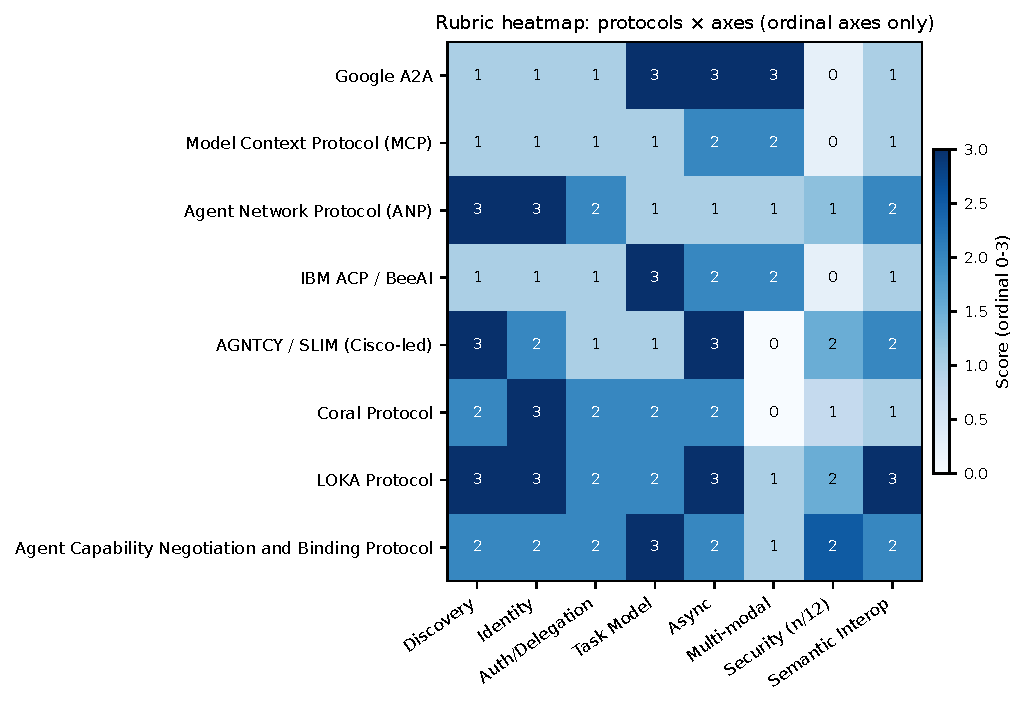
\includegraphics[width=0.85\textwidth]{figures/fig5-heatmap.pdf}
  \caption{Rubric heatmap across protocols and axes. Colour
  encodes the ordinal score for axes 1 to 3, 5 to 7, and 9;
  axes 4, 8, and 10 are summarized as described in
  \S\ref{sec:rubric}. Empty rows are pending per-protocol
  evidence notes for the two placeholder protocols (IBM ACP,
  AGNTCY/SLIM); the five commerce-settlement protocols are
  scored separately in Table~\ref{tab:commerce-stack}. The
  matrix is regenerated mechanically
  from \texttt{data/protocol-scores.yaml} by
  \texttt{scripts/gen\_heatmap.py}.}
  \label{fig:heatmap}
\end{figure*}

\begin{figure*}[!ht]
  \centering
  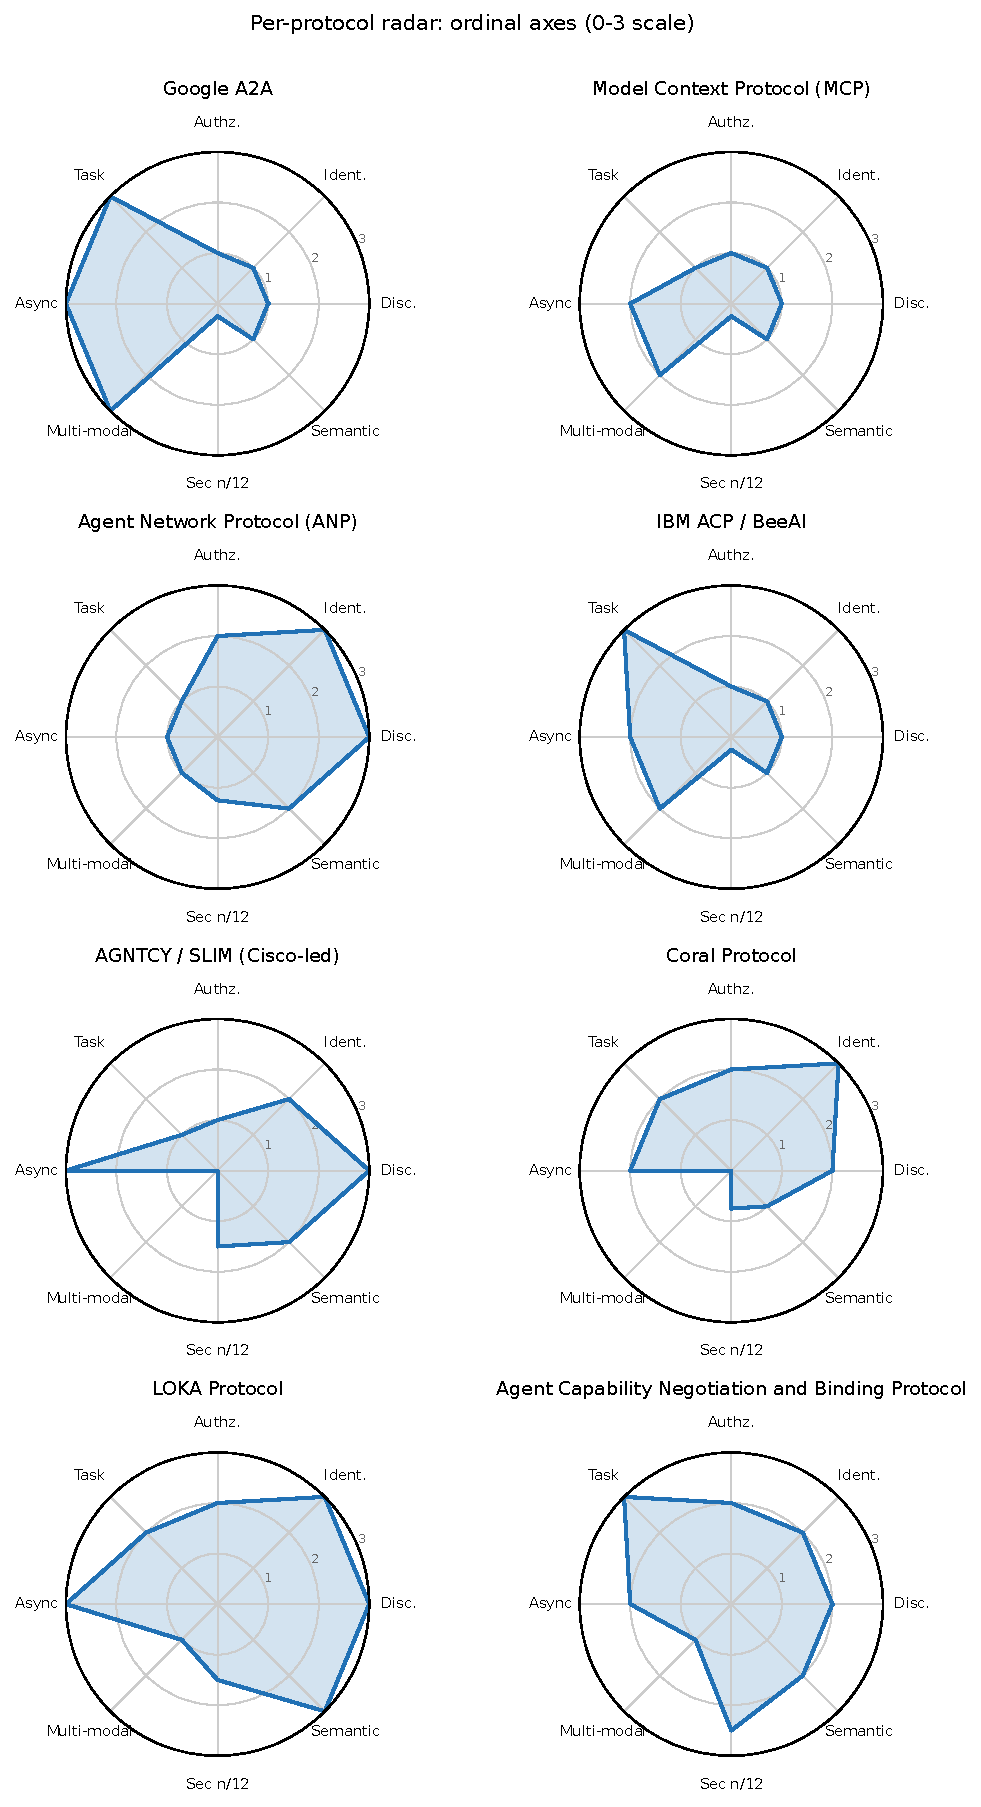
\includegraphics[width=0.75\textwidth]{figures/fig6-radar.pdf}
  \caption{Per-protocol radar charts on the seven ordinal
  axes (1 to 3, 5 to 7, 9) plus a normalized Axis 8 threat
  count. Each polygon describes a protocol's profile across
  the rubric; the heatmap (Figure~\ref{fig:heatmap})
  presents the same data as a colour matrix for
  cross-protocol comparison. Regenerated by
  \texttt{scripts/gen\_radar.py}.}
  \label{fig:radar}
\end{figure*}

\paragraph{The Axis 9 gap is structural.}
No surveyed protocol scores 3 on semantic interoperability.
LOKA's score of 3 is explicitly aspirational; the
Polyglot Intent Engine is a proposed mechanism rather than
a shipped one. Five protocols (A2A, MCP, ACP, Coral, and
the Axis-9 aspect of AGNTCY) cluster at 1 (free-text
descriptions over typed schemas). ANP at level 2
(JSON-LD with ADP) is the only protocol that
\emph{ships} an ontology-base mechanism. The gap is
discussed in detail in \S\ref{sec:semantic}; the rubric
makes precise that the LLM-era flexibility we celebrated
in \S\ref{sec:background:llm-disruption} has come at a
documented cost on this axis.

\subsection{How each score was assigned: per-axis derivation}
\label{sec:comparison:derivation}

This subsection walks every axis in Table~\ref{tab:rubric-matrix}
and explains, cell-by-cell, what specification evidence
anchored each scored protocol at the level shown. The
methodology is the four-step procedure of
\S\ref{sec:rubric:method}: identify the spec section
relevant to the axis, map its behaviour to the anchored
descriptors of \S\ref{sec:rubric:axes}, record the
resulting score, and write the evidence summary. Each
paragraph below corresponds to one column of the
comparison matrix. The companion repository's
\texttt{data/protocol-scores.yaml} carries the
machine-readable form of every evidence sentence quoted
here, with the spec citation key attached.

\paragraph{Axis 1 (Discovery and Registry Model).}
Recall the anchored descriptors of \S\ref{sec:rubric:axis1}:
0 = out-of-band only; 1 = well-known endpoint; 2 =
federated directory with structured descriptors; 3 =
decentralized verifiable resolution. \textbf{A2A scores 1}
because its discovery primitive is the well-known endpoint
\texttt{/.well-known/agent-card.json}~\cite{spec_a2a};
trust is delegated to the hosting authority and no
verifiable cryptographic resolution is provided.
\textbf{MCP also scores 1}: the spec defines
server-config-mediated discovery with an emerging registry
that is, at the cutoff, mostly out-of-band~\cite{spec_mcp};
the level-1 anchor (configuration mediated) fits more
naturally than level 0. \textbf{ANP scores 3}: the white
paper specifies a DID resolver paired with the Agent
Description Protocol, returning cryptographically
verifiable descriptors independent of any single
authority~\cite{spec_anp}. \textbf{Coral scores 2}: the
\texttt{list\_agents} MCP tool resolves names from a
server-mediated Coral Server; the resolution is
blockchain-anchored but server-mediated rather than
DID-based~\cite{spec_coral}, fitting the federated-directory
anchor. \textbf{LOKA scores 3}: its Semantic Discovery
Fabric (\S3.2 of the LOKA white paper) plus the proposed
\texttt{did:loka:} resolver in \S4.1 match the
decentralized-verifiable-resolution descriptor~\cite{spec_loka};
the score is aspirational, as flagged in
\S\ref{sec:rubric:limits}, but the specification text
supports the level. \textbf{ACNBP scores 2}: Definition~4
of the spec defines the Agent Name Service as a
DNS-like federated directory maintaining Agent Network
Resource Identifiers~\cite{spec_acnbp}; federated but not
DID-based, hence level 2.

\paragraph{Axis 2 (Identity and Authentication).}
Anchors of \S\ref{sec:rubric:axis2}: 0 = process trust or
unspecified; 1 = bearer tokens (OAuth-style); 2 = bearer
tokens hardened with mTLS or signed envelopes; 3 = DIDs
with verifiable credentials. \textbf{A2A scores 1}: OAuth
2.x is documented in the AgentCard schema; mTLS and JWT
are supported but not mandated, and the spec does not
require message-level signing~\cite{spec_a2a, a2a_weaknesses}.
\textbf{MCP scores 1}: OAuth 2.1 is the HTTP-transport
identity mechanism; the stdio transport relies on
parent-process trust, which the rubric records as a
level-1 hybrid in the evidence field~\cite{spec_mcp}.
\textbf{ANP scores 3}: identity is established by DIDs
plus W3C Verifiable Credentials, the rubric's level-3
anchor~\cite{spec_anp}. \textbf{Coral scores 3}: each
agent holds a DID with cryptographic credentials, and
Solana wallets serve as the authenticator (\S7 of the
Coral paper)~\cite{spec_coral}, matching the
DID-with-VC anchor. \textbf{LOKA scores 3}: \S4.1
specifies DID documents with Ed25519 keys plus VCs with
issuer/subject/verifier roles and a Dilithium post-quantum
upgrade path~\cite{spec_loka}. \textbf{ACNBP scores 2}:
identity rests on X.509 certificates with OCSP revocation
and ECC-signed envelope structures (\S\S III.A, IV.A,
VII.B)~\cite{spec_acnbp}; DIDs are not native, but the
combination of signed envelopes with PKI matches the
level-2 anchor, not level 3.

\paragraph{Axis 3 (Authorization and Delegation Model).}
Anchors of \S\ref{sec:rubric:axis3}: 0 = unspecified; 1 =
scope tokens, or no standardised delegation credential;
2 = VC-scoped
capabilities or structured delegation tokens; 3 =
cryptographically-bound capability chains. \textbf{A2A
scores 1}: the spec advertises authentication schemes in
the AgentCard and defines an in-task authorization flow
(\S7.6) with an auth-required task state, but standardises
no delegation credential. \S7.5 makes authorization logic
implementation-specific~\cite{spec_a2a}. The in-task flow
re-acquires a credential at the boundary rather than
carrying a verifiable chain, so the receiver still holds a
bearer credential with no chain of custody behind it. That
is the level-1 anchor. Deployments close the gap with
token forwarding, which the security literature observes
in production~\cite{authz_propagation}; the pattern is
attributable to deployments, not to the specification. \textbf{MCP
scores 1}: OAuth scopes only; no agent-delegation
primitive in the cutoff spec~\cite{spec_mcp}.
\textbf{ANP scores 2}: VC-scoped capabilities are
supported and cryptographic chains are possible in
principle, but the chain-of-custody pattern is not fully
standardized~\cite{spec_anp}. \textbf{Coral scores 2}:
\S7 defines Team Contracts as signed multi-agent
agreements (optionally on-chain); this is a partial
delegation chain, not yet at the level of RFC
8693~\cite{rfc8693} or better~\cite{spec_coral}.
\textbf{LOKA scores 2}: VCs act as scoped capability
attestations (\S4.1) and smart-contract lifecycle
policies (\S3.1) carry the policy layer; no RFC 8693
mapping~\cite{spec_loka}. \textbf{ACNBP scores 2}:
Definition~10 defines Capability Binding as a
cryptographically-bound, mutually-signed commitment
backed by a capability attestation (Def.~14) with
immutable audit trails~\cite{spec_acnbp}. This is the
most rigorous single-hop authorization primitive in the
surveyed set, and it is single-hop. Definition~10 binds a
requester agent to a provider agent, two named parties.
The specification does not extend the binding to a third
party, and its text contains no treatment of delegation,
authorization propagation, or acting on behalf of another
principal. A lead author confirmed in correspondence that
ACNBP is a two-party negotiation-and-binding protocol and
that multi-agent delegation is outside its scope. So the
level-3 clause requiring an intermediate agent's
authorization to be independently verifiable is
unsatisfied, and the cell records level 2. This is the
last ordinal-3 the Axis 3 column had, and with it the
column tops out at 2
(\S\ref{sec:emerging:acnbp} gives the full derivation).

\paragraph{Axis 4 (Transport and Wire Format).}
Recall this axis is a tuple rather than an ordinal score
(\S\ref{sec:rubric:axis4}). The cells record what the
specification declares, not what implementations support.
A2A: HTTPS/JSON-RPC 2.0 with optional gRPC and REST,
JSON serialization, SSE streaming, push
notifications~\cite{spec_a2a}. MCP: stdio, HTTP+SSE, and
streamable-HTTP bindings; JSON-RPC 2.0 serialization;
SSE or chunked HTTP streaming; notifications plus
emerging MCP Tasks~\cite{spec_mcp}. ANP: HTTPS only;
JSON-LD over JSON; no native streaming; polling for
async~\cite{spec_anp}. Coral: HTTP / WebSocket / SSE;
JSON-via-MCP; SSE streaming; push via
\texttt{wait\_for\_mentions}~\cite{spec_coral}. LOKA:
\texttt{unspecified} on every sub-field. The paper
declares intent-centric peer-to-peer messaging
without committing to a transport binding~\cite{spec_loka}.
ACNBP: unspecified at the link layer (the spec is
transport-agnostic), JSON serialization
(RFC 7159~\cite{rfc7159}), no
in-protocol streaming, and a 10-step asynchronous
negotiation with encrypted session and forward
secrecy~\cite{spec_acnbp}. The tuple values are
transcribed verbatim from the spec sections cited in
the YAML evidence field; transcription is the only
rubric methodology for this axis. The RFC 7159 reference
is the specification's own, and it is stale: RFC 8259
obsoleted that revision in 2017.

\paragraph{Axis 5 (Task and Conversation Model).}
Anchors of \S\ref{sec:rubric:axis5}: 0 = stateless
request/response; 1 = session-scoped but no task object;
2 = persistent multi-participant interaction; 3 = full
task object with lifecycle, artifacts, and sub-task
delegation. \textbf{A2A scores 3}: the \texttt{Task}
object carries a lifecycle (submitted, working,
input-required, completed, failed, canceled), Parts and
Artifacts content aggregation, and explicit sub-task
delegation~\cite{spec_a2a}. \textbf{MCP scores 1}:
request/response with session-scoped state; the emerging
MCP Tasks extension begins to push toward level 2 but
is post-cutoff~\cite{spec_mcp}. \textbf{ANP scores 1}:
multi-turn interaction is supported, but a task is not a
protocol-level concept~\cite{spec_anp}. ANP's first-class
concepts are Information and Interface, and a task is
treated as one form of an Interface, on the argument that
the task abstraction is not general enough to carry every
interaction (\S\ref{sec:industry:anp}). The level records
the absence of the object, not an unfinished lifecycle. \textbf{Coral
scores 2}: stateful persistent multi-participant threads
are first-class; sub-task delegation is deferred to a
future Task Management service (\S7)~\cite{spec_coral}.
\textbf{LOKA scores 2}: the ALMS lifecycle (Genesis,
Growth, Crisis, Sunset) in \S3.1 covers agent lifecycle;
sub-task delegation is discussed in \S4.4.3 but is not a
first-class task primitive~\cite{spec_loka}.
\textbf{ACNBP scores 3}: the ten-step state machine of
the spec, with Protocol State (Def.~15) as a first-class
object, binding commitments that produce artifacts, and
multi-agent orchestration with capability composition
(\S IV.A), matches the level-3 anchor~\cite{spec_acnbp}.

\paragraph{Axis 6 (Async and Long-Running Operations).}
Anchors of \S\ref{sec:rubric:axis6}: 0 = no async; 1 =
polling-based; 2 = server-initiated notifications; 3 =
durable resumable tasks. \textbf{A2A scores 3}: push
notifications combine with polling and durable resumable
tasks; on reconnect the client receives a complete or
partial result and any backfilled events~\cite{spec_a2a}.
\textbf{MCP scores 2}: notifications plus emerging MCP
Tasks; durability across connection loss is not yet a
cutoff-specification feature~\cite{spec_mcp}. \textbf{ANP
scores 1}: polling primarily; the white paper does not
specify a push-notification standard~\cite{spec_anp}.
Asynchrony is left to the individual Interface to define
rather than raised to a protocol-level primitive, so the
level reflects a scoping decision
(\S\ref{sec:industry:anp}).
\textbf{Coral scores 2}: \texttt{wait\_for\_mentions} is
an explicit push primitive (\S6.1.2); durable-resumable
semantics are not specified~\cite{spec_coral}.
\textbf{LOKA scores 3}: \S3.1 specifies Crisis-phase
continuous checkpointing, redundancy overlays, and
recovery via verifiable snapshots, matching the
durable-resumable anchor (aspirationally)~\cite{spec_loka}.
\textbf{ACNBP scores 2}: \S IV.A specifies
subscription-based capability update notifications;
durable-resumable bound execution is not
specified~\cite{spec_acnbp}.

\paragraph{Axis 7 (Multi-Modal Content Handling).}
Anchors of \S\ref{sec:rubric:axis7}: 0 = plain text;
1 = text plus referenced attachments; 2 = typed content
blocks; 3 = typed parts with inline-or-reference duality.
\textbf{A2A scores 3}: TextPart, FilePart, and DataPart
with inline and URL-reference modes are the canonical
level-3 vocabulary~\cite{spec_a2a}. \textbf{MCP scores
2}: typed content blocks (text, image, resource) plus
structured JSON-Schema tool input fit the level-2
anchor~\cite{spec_mcp}; level 3 would require explicit
content negotiation. \textbf{ANP scores 1}: text plus
file references; no typed parts model~\cite{spec_anp}.
\textbf{Coral scores 0}: natural-language message content
with mention metadata only; no typed parts, file
references, or content negotiation
schema~\cite{spec_coral}. This is the lowest score on
Axis 7 in the surveyed set and the largest single weak
spot in Coral's profile. \textbf{LOKA scores 1}: the
DID document defines a CredentialRepositoryService with
a service endpoint URL (\S4.1); typed inline multimodal
parts are not specified~\cite{spec_loka}. \textbf{ACNBP
scores 1}: capabilities define typed input/output
parameters (Def.~2) but the spec does not specify
inline multimodal parts or streaming media~\cite{spec_acnbp}.

\paragraph{Axis 8 (Security Threat Surface).}
This axis is a count over the fixed twelve-item threat
catalogue of \S\ref{sec:rubric:axis8}. Counts are the
number of threats that the specification \emph{explicitly}
addresses at the spec level, not at the deployment level.
A mitigation that the specification recommends without
requiring scores \emph{partial} and does not enter the
count, which is why several counts here are lower than a
reading of the same protocol's security section suggests.
\textbf{A2A: 3 partial, 1 of 12 addressed}: transport
encryption is the sole spec-level mitigation. OAuth bearer
identity, push-notification replay verification, and
transport-layer DoS resistance are real but partial:
the AgentCard itself is unsigned. Injection, AgentCard
supply-chain attacks,
registry poisoning, and delegation token theft are
explicitly identified as out-of-spec in the
literature~\cite{a2asecbench, a2a_weaknesses, spec_a2a}.
\textbf{MCP: 2 partial, 1 of 12 addressed}: TLS on the HTTP
transport is the sole spec-level mitigation. OAuth 2.1
identity is partial because the stdio transport substitutes
process trust, and token expiry is the only replay defence.
Indirect injection and tool poisoning are
documented as unaddressed~\cite{zhan2024injecagent,
protocol_exploits, spec_mcp}. Two classes are not
applicable, since MCP is agent-to-tool rather than
peer-to-peer. \textbf{ANP: 5 of 12}:
identity, authentication, integrity, audit, and
non-repudiation are addressed through DIDs and VCs;
prompt injection, registry poisoning, and capability
escalation remain unaddressed~\cite{spec_anp}.
\textbf{Coral: 3 partial, 3 of 12 addressed}: DIDs and Solana wallet
authentication, on-chain immutable audit, and thread-scoped
privilege confusion are addressed. Team-contract capability
escalation and delegation token theft are partial, and so is
message integrity, because the on-chain signatures cover the
payment path and not the message path. Replay, supply-chain,
side-channel, DoS, prompt injection, and registry poisoning are
not addressed~\cite{spec_coral}. \textbf{LOKA: 4 partial, 6 of 12 addressed}:
DID-and-Dilithium authentication, timestamp-and-signed-intent
replay, blockchain audit, post-quantum MITM,
decentralized-SSI registry, and Contextual Ethics privilege
confusion are addressed. The DECP prompt-injection filter,
VC-and-contract capability scoping, delegation token
binding, and the Contextual Ethics privacy policies are
partial, so they do not enter the count. Supply-chain and
DoS are not addressed~\cite{spec_loka}. \textbf{ACNBP: 10 of
12}: the MAESTRO 7-layer analysis (\S VII.I) explicitly
addresses ZKP capability attestation, signature plus HMAC
integrity, rate-limit-plus-PoW DoS mitigation,
nonce-and-timestamp-and-sequence replay defence,
\texttt{protocolExtension} whitelist supply-chain
defence, X.509 plus OCSP impersonation defence, the
Capability Binding ceremony against delegation-token
theft, signed-ANRI plus BFT registry integrity,
foundation-model prompt-injection mitigation, and
cryptographically protected audit logs~\cite{spec_acnbp}.
Two classes score partial and do not enter the count:
side-channel privacy, offered through ring signatures,
and cross-agent privilege confusion, offered through
agent quarantine. The count is the
highest in the surveyed set; \S\ref{sec:security} returns
to the question of how to read a high count when the
underlying spec lacks production deployment.

\paragraph{Axis 9 (Semantic Interoperability).}
Anchors of \S\ref{sec:rubric:axis9}: 0 = free-text only;
1 = structured schemas with free-text descriptions; 2 =
ontology-base or semantic-discovery indexing; 3 = full
capability ontology with semantic matching. \textbf{A2A
scores 1}: typed Skill objects pair with free-text
descriptions and no ontology alignment~\cite{spec_a2a}.
\textbf{MCP scores 1}: JSON Schema for tool input with
free-text natural-language tool descriptions~\cite{spec_mcp}.
\textbf{ANP scores 2}: JSON-LD as the serialization
provides an ontology base, and ADP enables semantic
discovery~\cite{spec_anp}; the only ordinal-2 on Axis 9
in the surveyed set. This is the one cell in the matrix
that a post-cutoff revision would move
(\S\ref{sec:semantic:ontology}). \textbf{Coral scores 1}: Coraliser
adapters enforce uniform schemas (\S6.3) but the spec
does not specify a formal capability descriptor or
ontology~\cite{spec_coral}. \textbf{LOKA scores 3}: the
combination of capability ontologies, intent schemas,
ethical inheritance (\S3.1) and the Polyglot Intent
Engine targeting FIPA-ACL / A2A / Open Voice
(\S4.5.2)~\cite{spec_loka} matches the full-ontology
anchor aspirationally. The engine is not yet
implemented. \textbf{ACNBP scores 2}: Definition~2
provides a structured capability descriptor; \S IV.D
specifies a Semantic Consistency Check; ontology-based
classification (\S VIII.A) is recommended as a future
enhancement~\cite{spec_acnbp}.

\paragraph{Axis 10 (Governance, License, and Observability).}
The composite triple of \S\ref{sec:rubric:axis10} is
recorded by transcription rather than scoring for the
first two sub-fields; only the third (observability) is
ordinal. \textbf{A2A}: Linux Foundation steward, Apache
2.0 licensed, observability 2 (SSE event stream supports
tracing; no standardized audit
primitives)~\cite{spec_a2a, lf_aaif}. \textbf{MCP}:
Linux Foundation AAIF steward, MIT-equivalent licensed,
observability 1 (logging hooks emerging; no standardized
audit primitives)~\cite{spec_mcp, lf_aaif}.
\textbf{ANP}: community / W3C-aligned steward, Apache
2.0 licensed, observability 1 (built-in non-repudiation
logs; no standardized audit dashboard)~\cite{spec_anp,
w3c_agent_protocol_cg}. \textbf{Coral}: Coral Protocol
team steward, CC-BY-4.0 paper license, observability 2
(mandatory blockchain audit trail for payments and team
contracts in \S8; no separate trace or metric
spec)~\cite{spec_coral}. \textbf{LOKA}: academic-authors
steward (CMU Tepper / BIT Sindri) with no formal SDO,
CC-BY-NC-SA 4.0 licensed, observability 3 (\S5.1
specifies immutable audit trails, real-time ethical
auditing, and blockchain-ledger action and reasoning
records)~\cite{spec_loka}. \textbf{ACNBP}:
individual-authors steward (DistributedApps.ai, Cisco,
OWASP/AWS, Intuit) with no formal SDO, CC-BY 4.0
licensed, observability 3 (\S IV.H specifies
cryptographically protected audit logs, comprehensive
event logging, privacy-preserving logging, and
integration with external audit/compliance
systems)~\cite{spec_acnbp}. The composite is not
aggregated into a single number, by D3 of
\S\ref{sec:rubric:goals}; \S\ref{sec:governance} treats
governance as the most decisive of the three sub-fields
for protocol survival.

\paragraph{Contestable boundary calls.}
Four cells in Table~\ref{tab:rubric-matrix} sit at
contestable boundaries that a reader may dispute. \textbf{A2A on Axis 1.} A reader
who classes the AgentCard convention as a federation
rather than a hosted convention could plausibly raise
A2A to level 2; we score 1 because no central registry
is specified and the convention is implemented by each
host individually. \textbf{ANP on Axis 3.} A reader who
treats VC-scoped capabilities plus the implicit
cryptographic chain as a complete level-3 mechanism
could raise ANP to 3; we score 2 because the
chain-of-custody format is not standardized in the
white paper and no reference profile of the chain has
been published. \textbf{Coral on Axis 2.} A reader could
plausibly score Coral at 2 (signed envelopes via Solana
wallet signatures) rather than 3 (DIDs and VCs) by
arguing that the wallet signature is the operative
identity primitive and the DID is decorative; we score 3
because the spec text in \S7 establishes the DID as the
primary identifier and the wallet as the cryptographic
authenticator over it. \textbf{ACNBP on Axis 3.} A reader
who treats the capability-binding ceremony as satisfying
the level-3 anchor's parenthetical could score ACNBP at 3,
and an earlier version of this survey did. We score 2
because the anchor's operative clause is the one after the
parenthetical: an intermediate agent's authorization must
be independently verifiable, and Definition~10 binds only
two parties. A lead author confirmed the two-party reading
in correspondence, which agrees with the specification
text. This is the only cell in the matrix whose score
changed after correspondence with a protocol's authors,
and it is recorded as such in the YAML. Each of these
calls is flagged in the YAML evidence field so future
readers can re-litigate them against the
\texttt{spec\_version}/\texttt{retrieved} pair in effect.



\subsection{Clusters: registry-anchored, DID-anchored, commerce-settlement}
\label{sec:comparison:clusters}

The rubric matrix renders three protocol clusters that no
prior survey identified as architecturally distinct.

\paragraph{Cluster 1: Registry-anchored.}
A2A, MCP, ACP, AGNTCY, and Coral share the structural
assumption that an agent's existence and capabilities are
mediated by a discovery service (a well-known endpoint, a
federated directory, a server-mediated capability list).
The cluster's defining trade-off is operational
maturity for decentralization properties: registry-anchored
protocols are easier to deploy in a single-organization or
single-foundation context (\S\ref{sec:industry-protocols})
and harder to deploy across organizational trust
boundaries without negotiating registry federation.
Rubric signature: Axis 1 scores of 1 to 2, Axis 2 scores
of 1 (with the exception of Coral at 3, by way of its
Solana-wallet authenticator), governance under a foundation
or vendor consortium (A10 governance sub-field).

\paragraph{Cluster 2: DID-anchored.}
ANP and LOKA share the structural assumption that an
agent's identity, location, and authorizations are
expressed as a decentralized identifier resolvable
independently of any single registry. The cluster's
defining trade-off is the inverse of Cluster~1:
decentralization properties for operational maturity. The
DID-anchored protocols score 3 on Axis 1 (decentralized
verifiable resolution) and Axis 2 (DIDs and VCs), but
their task-and-content layers are less developed than
A2A's. ANP's Axis 5 score of 1 and Axis 6 score of 1
(polling-only async) reflect this gap directly.

\paragraph{Cluster 3: Commerce-settlement.}
AP2, Visa TAP, Mastercard Agent Pay, and ERC-8004 form a
co-stack rather than a competition (\S\ref{sec:emerging:commerce}).
UCP sits above them and orchestrates the transaction that
surrounds the payment. All five sit outside the
peer-messaging rubric matrix by
design and are compared separately in
Table~\ref{tab:commerce-stack}: the architectural
primitive (the intent-mandate-receipt envelope)
positions them identically with respect to Axis 3 (where
the commerce-settlement layer establishes the rigour the
peer-messaging layer has not yet matched), Axis 5 (where
the unit of interaction is a triple rather than a
multi-message task), and Axis 7 (where multi-modal handling
is not applicable). The cluster is best understood as
\emph{layer 3} of the three-layer taxonomy
(\S\ref{sec:taxonomy:layers}) rather than as a fourth
peer-messaging cluster.

\paragraph{ACNBP as a bridge.}
ACNBP does not fit cleanly into any of the three clusters.
Its Axis 1 score of 2 places it nearer Cluster~1
(registry-anchored, via the ANS directory) than Cluster~2.
Its capability-binding ceremony borrows the
commerce-settlement layer's discipline of signing an
authorization rather than forwarding a token, though it
stops at two parties and so scores 2 rather than 3 on
Axis 3. The protocol is best read as a partial import of
the commerce-settlement layer's authorization rigour into
the peer-messaging layer: the ceremony crosses over, the
chain of custody does not. The ten-step state machine
plays the role of an explicit cryptographic negotiation
that the industry-led peer-messaging protocols have left
implicit.

\subsection{Where protocols overlap and where they stack}
\label{sec:comparison:stack}

The taxonomy of \S\ref{sec:taxonomy} argued that
contemporary protocols compose rather than compete; the
rubric matrix lets us identify the specific composition
boundaries.

\paragraph{MCP + A2A.}
The canonical stack of \S\ref{sec:taxonomy:complementary}.
MCP provides the tool-binding layer for each A2A agent;
A2A provides the inter-agent task semantics above the
tool layer. The rubric scores are complementary: MCP's
Axis 7 score of 2 (typed content blocks) is sufficient
for tool-call payloads, while A2A's Axis 7 score of 3
covers the richer inter-agent message content. MCP's
Axis 5 score of 1 is irrelevant once A2A's score of 3
carries the task semantics. The pair has no axis
on which they fight, and at least three axes (5, 6, 7)
on which the lower-scoring layer borrows the
higher-scoring layer's primitives.

\paragraph{Coral + MCP.}
Coral~\cite{spec_coral} ships this composition
explicitly: tool integration is MCP-mediated, while
Coral's persistent threads occupy the peer-messaging
layer. The composition is structurally identical to
A2A + MCP modulo the task-versus-thread choice on
Axis 5 (Coral's 2 versus A2A's 3) and the multi-modal
gap on Axis 7 (Coral's 0 is a real cost; an A2A
companion layer would supply Axis 7 in a
Coral-deployed setting).

\paragraph{ANP + A2A (potential).}
The matrix renders a natural pairing: ANP's
identity-layer strengths complement A2A's
task-layer strengths. That pairing is not yet a deployed stack at
the cutoff. The composition would require an
identity-bridge specifying how a DID-resolved agent
presents itself across an A2A AgentCard, and the AAIF
working group has begun work on the bridge but has not
published a specification. This pairing is the
single composition that the rubric most clearly
recommends and that the industry has not yet
shipped.

Two qualifications keep the recommendation honest, and both
follow from how ANP is built. ANP is a stack of
sub-protocols rather than one document, so the composition
is a claim about some of its parts and not all of them. The
DID mechanism is the portable part: it carries no
dependency on the rest of ANP and could in principle sit
under A2A directly. The other parts do not compose as
cleanly. ANP's Agent Description and Agent Discovery
protocols overlap substantially with what the A2A
AgentCard already does, so a deployment adopting both would
carry two descriptor formats for one purpose and would have
to choose which is authoritative. The recommendation is
therefore narrower than the protocol pair suggests: adopt
ANP's identity layer beneath A2A's task layer, and treat
description and discovery as a place where the two
specifications compete rather than stack. That narrowing
strengthens the case rather than weakening it. The
identity mechanism is separable, which is the property
\S\ref{sec:governance:survival} argues predicts adoption,
and it is the layer where A2A scores 1 and has the most
to gain.

\paragraph{Commerce-settlement + peer-messaging.}
The intent-mandate-receipt envelope of the
commerce-settlement layer stacks above any
peer-messaging protocol that can carry it as a typed
content part. A2A's DataPart and Coral's
mention-metadata both provide adequate transport. The
AAIF Agentic Commerce Working
Group~\cite{lf_aaif} has begun harmonizing the
envelope schema across AP2, Visa TAP, Mastercard
Agent Pay, and ERC-8004, with the explicit goal that
a single agent's mandate be portable across
peer-messaging substrates. The matrix's commerce-settlement
rows will populate as that harmonization yields
public specifications.

UCP is the one deployed instance of this composition at the
cutoff. It declares MCP and A2A as two of its four transport
bindings and consumes AP2's mandate as an optional extension
(\S\ref{sec:emerging:commerce}). The stack that this
subsection argues for is therefore not hypothetical at the
commerce layer. The parties who built it had no stake in the
argument.

\paragraph{The principal overlap: ACP versus MCP at
the tool-binding layer.}
On only one axis do two surveyed protocols directly
compete, in the sense of occupying the same layer with
incompatible wire formats. That axis is the tool-binding layer
between ACP and MCP. The rubric scores them similarly on
most axes (ACP's placeholder row hides this, but the
specification-level reading puts them within one level on
identity, authorization, and async); the operational
difference is ACP's REST+multipart serialization versus
MCP's JSON-RPC 2.0. The market has overwhelmingly chosen
MCP; the survey records ACP's existence and design choices
without expecting them to displace the MCP baseline within
the cutoff horizon.

\paragraph{Where the literature has been wrong.}
Several published commentaries~\cite{ehtesham2025interop,
yang2025survey, protocolbench} have framed A2A versus
MCP, A2A versus ANP, or A2A versus Coral as direct
competitions. The rubric matrix makes precise that these
framings are category errors. A2A and MCP occupy
different layers (\S\ref{sec:taxonomy:complementary}).
A2A and ANP have complementary strengths and would
compose naturally if a bridge existed (above). A2A and
Coral occupy the same peer-messaging layer with
different conversational primitives (task versus
thread) and can interoperate through translator
adapters of the kind Coral's Coraliser provides for MCP.
The clearest contribution of the rubric matrix is that
it renders these architectural distinctions visible
where the prior surveys' qualitative comparisons left
them ambiguous.

\section{Security and Threat Surface}
\label{sec:security}

This section synthesises the security and threat-modelling
literature on inter-agent protocols and applies the twelve-class
threat catalogue introduced as Axis 8 of the rubric
(\S\ref{sec:rubric:axis8}) protocol-by-protocol.
Section~\ref{sec:security:model} fixes a composite threat model
covering the four principal entities of a contemporary agentic
deployment (user, orchestrator, remote agent, tool or MCP
server) and identifies where on that model each of the twelve
threat classes manifests.
Section~\ref{sec:security:identity} to \ref{sec:security:tee}
each treat one major threat category in depth, drawing on the
specification-level coverage in
Table~\ref{tab:threat-surface} and the empirical and analytical
literature catalogued in our references.
Section~\ref{sec:security:open} closes with the unresolved
problems that should drive the next standardisation cycle.
Half of these reappear in \S\ref{sec:openproblems} as the
top-priority items on the survey's open-problems agenda.

This is deliberately \emph{not} a re-derivation of the security
literature (\S\ref{sec:intro:notwhat}, D3). Kong et
al.~\cite{kong2025communication} already provide a 48-page
treatment that is the canonical primary source for the field.
What \S\ref{sec:security} adds is the spec-coverage view: a
matrix that says, for each protocol's published
specification at the 2026-Q1 cutoff, which threats the spec
addresses with normative language, which it acknowledges only
in non-normative recommendations, and which it leaves out of
scope entirely.

\subsection{Composite threat model}
\label{sec:security:model}

The threat model spans four entities and the three edges
between them. The model is consistent with the layered
architectures of
Kong~\cite{kong2025communication}, A2ASecBench~\cite{a2asecbench},
and the threat-modelling survey~\cite{threatmodel2026}, and
serves as the geometry against which we locate each of the
twelve threat classes.

\begin{description}
  \item[Entity 1: User principal.] A human or
    organisational identity on whose behalf an orchestrator
    is acting. The principal authorises specific intents and
    delegates a bounded mandate to the orchestrator. Threats:
    cross-tenant identity confusion, principal-impersonation
    via stolen mandates, mandate-replay across delegation
    boundaries.
  \item[Entity 2: Orchestrator agent.] The primary
    agent (typically an LLM with an associated runtime)
    that holds the principal's mandate and selects which
    remote agents or tools to invoke. Threats:
    prompt injection at the principal-orchestrator
    boundary, orchestrator output validating
    a downstream attack, side-channel leakage through
    orchestrator logs.
  \item[Entity 3: Remote agent.] A peer agent reached
    via A2A, ANP, AGNTCY/SLIM, Coral, or an equivalent
    peer-messaging substrate. Threats: agent impersonation,
    AgentCard supply-chain attacks, capability escalation
    through ambiguous Skill descriptions, registry poisoning
    against the discovery convention.
  \item[Entity 4: Tool or MCP server.] A
    capability-providing endpoint reached via MCP or an
    equivalent tool-binding protocol. Threats: tool
    poisoning, indirect prompt injection through tool
    results, malicious schema in tool input contracts,
    confused-deputy attacks where the orchestrator's
    OAuth scope is exceeded by tool calls it doesn't
    authorise.
\end{description}

The three edges carry the messages on which all
twelve threats land: principal-to-orchestrator,
orchestrator-to-remote-agent, and
orchestrator-to-tool. Twelve threats is the smallest count
that lets every one of the six published threat-modelling
papers~\cite{kong2025communication, a2asecbench,
threatmodel2026, protocol_exploits, a2a_weaknesses,
zhan2024injecagent} map onto a single matrix without
hiding a threat under an unrelated heading; the granularity
is set by the literature, not by the survey's preferences.

\clearpage

Table~\ref{tab:threat-surface} presents the matrix.
Eight of the twelve threats land on multiple edges
simultaneously. Registry poisoning, for example, is an
attack against the discovery infrastructure. Its impact
flows along every edge that consumes a poisoned descriptor.
The matrix records the protocol's spec-level coverage of
each threat regardless of which edges that protocol mediates,
with the \texttt{na} marker reserved for threats that are
structurally outside the protocol's scope (e.g., MCP has no
AgentCard, so the AgentCard supply-chain row is
\texttt{na} for MCP).

% Generated by scripts/gen_table3.py: do NOT hand-edit.
% Source: data/threat-coverage.yaml.

\begin{table}[h!]
  \centering
  \caption{Threat-surface coverage matrix. Twelve threat classes (rows) $\times$ eight protocols (cols). Cells: \textbf{A} = Addressed at the spec level; P = Partial or non-normative; N = Not addressed; n/a = Not applicable. Every cell is scored against specification text. ACP and AGNTCY were rescored from primary sources in 2026-Q3: ACP against its OpenAPI document, which declares no security schemes; AGNTCY across its SLIM, OASF, Directory, and identity specifications.}
  \label{tab:threat-surface}
  \footnotesize
  \begin{tabular}{lcccccccc}
    \toprule
    Threat class & A2A & MCP & ACP & AGNTCY & ANP & Coral & LOKA & ACNBP \\
    \midrule
    Prompt injection (protocol boundary) & N & N & N & P & N & N & P & \textbf{A} \\
    Agent impersonation & P & P & N & \textbf{A} & \textbf{A} & \textbf{A} & \textbf{A} & \textbf{A} \\
    Message replay & P & P & N & \textbf{A} & \textbf{A} & N & \textbf{A} & \textbf{A} \\
    Capability escalation & N & N & N & N & N & P & P & \textbf{A} \\
    Delegation token theft & N & N & N & N & P & P & P & \textbf{A} \\
    Registry poisoning & N & N & N & \textbf{A} & \textbf{A} & N & \textbf{A} & \textbf{A} \\
    AgentCard supply-chain & N & n/a & N & \textbf{A} & n/a & n/a & N & \textbf{A} \\
    Message tampering / MITM & \textbf{A} & \textbf{A} & \textbf{A} & \textbf{A} & \textbf{A} & P & \textbf{A} & \textbf{A} \\
    Side-channel privacy leak & N & N & N & N & N & N & P & P \\
    Denial of service & P & N & N & P & N & N & N & \textbf{A} \\
    Cross-agent privilege confusion & N & n/a & N & \textbf{A} & N & \textbf{A} & \textbf{A} & P \\
    Audit-log tampering & N & N & N & P & \textbf{A} & \textbf{A} & \textbf{A} & \textbf{A} \\
    \bottomrule
  \end{tabular}
\end{table}


The matrix renders three structural observations, and a
fourth that only appears once the twelve classes are
weighted by how much each one costs.

\paragraph{The widely-deployed protocols cluster at one
addressed class each.}
A2A, MCP, and ACP each address exactly one of the twelve
classes, and in all three cases it is message tampering, via
transport encryption. A2A adds three partial mitigations and
MCP two, so the specifications are not silent on security;
they are non-normative about it. The reason is consistent
across the cluster: each protocol
specifies its identity and transport-encryption layers,
the identity layer without binding it cryptographically,
then relies on deployment-level mitigations
(WAFs, OAuth scopes, application-layer audit logging) for
the rest. AGNTCY is the counterexample that shows this is a
choice rather than a constraint of industry sponsorship: it
is equally industry-led and addresses six classes, because
MLS~\cite{rfc9420}, Sigstore signing~\cite{sigstore2022}, and
content addressing are specified
normatively rather than recommended. The literature
converges on the assessment that
the cluster's posture is the principal residual risk in
production: A2ASecBench~\cite{a2asecbench} reports
exploitable variants of nine of the twelve classes against
deployed A2A endpoints in its 2026 evaluation; the A2A
weakness analysis~\cite{a2a_weaknesses} catalogues eight
named threats against the same spec.

\paragraph{Decentralised-identity protocols invert the
profile.}
LOKA (6 addressed), ANP (5 addressed), and Coral (3
addressed) trade spec coverage of operational
threats for coverage of identity, authentication, and
audit-log threats via DIDs, Verifiable Credentials, and (in
Coral's and LOKA's cases) blockchain-anchored audit
trails. The cluster's weakness is the inverse: prompt
injection, capability escalation, delegation token theft,
and denial of service are unaddressed or only partial
throughout. Coral is the weakest of the three on the count
because its cryptographic guarantees attach to the payment
path rather than the message path. The
DIDs-and-VCs-for-agents paper~\cite{did_vc_agents} treats
this trade-off explicitly, framing it as the consequence of
specifying identity rigorously but leaving execution-time
threats to higher layers.

\paragraph{ACNBP is a positive outlier.}
ACNBP's ten of twelve addressed classes, with the remaining
two partial rather than absent (side-channel privacy via
ring signatures, and cross-agent privilege confusion via
agent quarantine), is the highest spec-level threat
coverage in the surveyed set, achieved by the explicit
MAESTRO seven-layer threat-modelling pass within the
specification (\S\ref{sec:emerging:acnbp})~\cite{spec_acnbp}.
ACNBP's deployment maturity is the lowest in the cluster:
the protocol exists at arXiv-draft stage with no
formal SDO. The design is still instructive. It shows what
specification-level threat coverage looks like when it is
written as part of the protocol rather than retrofitted
afterwards. \S\ref{sec:security:open} returns to ACNBP as
the model against which the industry-led protocols' threat
coverage gap should be benchmarked.

\paragraph{Severity-weighted coverage separates protocols
the count places together.}
The three observations above all read the matrix by
counting. Counting is the wrong instrument for the question
a deployer actually asks, which is how much risk is left
over. Table~\ref{tab:severity-coverage} reports the
severity-weighted view defined in \S\ref{sec:rubric:axis8}.
Each class carries a weight of 3, 2, or 1 by band. The
table reports addressed weight over applicable weight, and
the last column reports the unaddressed weight in the
critical and high bands alone.

% Generated by scripts/gen_table6.py: do NOT hand-edit.
% Source: data/threat-coverage.yaml (severity block).

\begin{table}[t]
  \centering
  \caption{Severity-adjusted threat coverage, the companion view to the Axis 8 count of Table~\ref{tab:threat-surface}. Bands and integer weights are declared in the companion repository, not computed here: 5 critical classes at weight 3, 5 high at weight 2, 2 moderate at weight 1, for 27 points across the twelve. Band columns read \emph{addressed / applicable}, where \texttt{na} classes are excluded from both. SWC is severity-weighted coverage: addressed weight over applicable weight. Residual is the unaddressed weight in the critical and high bands only, counting \texttt{partial} as unaddressed exactly as Axis 8 does. Higher SWC is better; lower residual is better.}
  \label{tab:severity-coverage}
  \footnotesize
  \begin{tabular}{lcccccr}
    \toprule
    Protocol & Axis 8 & Crit. & High & Mod. & SWC & Resid. \\
             & (of 12) & (w.\ 3) & (w.\ 2) & (w.\ 1) & & \\
    \midrule
    A2A & 1 & 0/5 & 1/5 & 0/2 & 7\% & 23 \\
    MCP & 1 & 0/5 & 1/3 & 0/2 & 9\% & 19 \\
    ACP & 1 & 0/5 & 1/5 & 0/2 & 7\% & 23 \\
    AGNTCY & 6 & 2/5 & 4/5 & 0/2 & 52\% & 11 \\
    ANP & 5 & 2/5 & 3/4 & 0/2 & 48\% & 11 \\
    Coral & 3 & 1/5 & 2/4 & 0/2 & 28\% & 16 \\
    LOKA & 6 & 2/5 & 4/5 & 0/2 & 52\% & 11 \\
    ACNBP & 10 & 5/5 & 4/5 & 1/2 & 89\% & 2 \\
    \bottomrule
  \end{tabular}
\end{table}


Three things follow that the count does not show. First,
the one-addressed cluster is worse off than its count
suggests. A2A, MCP, and ACP each address one class, and in
every case it is message tampering. That class sits in the
high band, not the critical one. All three therefore
carry zero of five critical classes. The two industry
protocols with the widest deployment leave 23 and 19 points
of critical-and-high weight unaddressed at the
specification level. Second, MCP's slightly higher
percentage is an artefact of scope, not of strength. Two
classes are \texttt{na} for MCP, so its denominator is
smaller, and the residual column is the fairer comparison.
Third, the gap between ACNBP and everything else widens
rather than narrows. ACNBP addresses all five critical
classes, so its residual is 2 against a field where the
next best is 11.

The parity that the count suggests between AGNTCY and LOKA
survives the reweighting. It is worth saying why, since
a weighting scheme that flattened every distinction would
be doing no work. Both address two of five critical classes
and four of five high, from different directions. AGNTCY
gets there through MLS, Sigstore signing, and content
addressing. LOKA gets there through DIDs, post-quantum
signatures, and a blockchain-anchored trail. The equal weighted score records
a real equivalence in residual risk, reached by
non-overlapping means.

The severity view does not rank protocols and is not
combined with any other axis. It answers one question the
count cannot, and it inherits the count's limits. It scores
specifications, not deployments. A specification that
addresses a critical class badly scores the same as one
that addresses it well.

\subsection{Identity and authentication}
\label{sec:security:identity}

Identity is the foundation on which every other security
property in inter-agent protocols rests, and the dimension
on which the contemporary protocols differ most. The rubric
matrix already records the three-way split
(\S\ref{sec:comparison:matrix}): industry-led protocols at
OAuth-bearer-token identity (Axis 2 score 1), ACNBP at
hardened-bearer-tokens-plus-PKI (Axis 2 score 2), and the
DID-anchored protocols at decentralised verifiable
identity (Axis 2 score 3).

\paragraph{The OAuth-bearer-token failure mode.}
A2A, MCP, and ACP all sit at OAuth-2.x identity. The
specification mandates bearer tokens issued by a third-party
authorisation server, with mTLS and JWT-with-signing as
optional hardenings. The empirical security
literature~\cite{a2asecbench, a2a_weaknesses} reports that
the optional hardenings are rarely used in the surveyed
deployments, and that bearer-token theft via downstream
log capture, browser cache leakage, or compromised
intermediaries is the most-frequent attack against deployed
A2A and MCP endpoints. The remediation under discussion in
the AAIF working group~\cite{lf_aaif} is to elevate the
mTLS-plus-message-signing pattern from optional to required
for production deployments, which would move A2A and MCP to
the rubric's Axis 2 level 2 in a future version.

\paragraph{The DID-anchored alternative.}
ANP, Coral, and LOKA all use W3C DIDs paired with Verifiable
Credentials (or, in Coral's case, Solana wallet signatures
over the DID). The advantage at the identity layer is
direct: a DID document carries the public keys necessary to
verify a challenge-response from the agent, and no
third-party authorisation server can be compromised to
issue tokens for an agent without the agent's
private-key cooperation. The
literature~\cite{did_vc_agents, spec_anp, spec_loka} reports
no published bypass of the
DID-plus-VC-challenge-response pattern; the residual risks
move down to private-key compromise (which is outside the
protocol scope) and to capability-layer attacks
(\S\ref{sec:security:authz}).

\paragraph{The PKI-hardened middle ground.}
ACNBP's X.509-plus-OCSP-plus-ECC envelope structure
\cite{spec_acnbp} sits between the OAuth and DID camps. The
operational advantage is compatibility with existing
enterprise PKI deployments; the operational disadvantage is
the cost of running an OCSP infrastructure that scales to
agent-population sizes. The literature is too thin to
report on real-world deployments of ACNBP's identity layer
because no such deployments exist at the cutoff; the
analysis here rests on the specification's own threat
model in \S VII of the ACNBP paper.

\paragraph{The protocol-level remaining problem.}
None of the contemporary protocols, including ACNBP,
addresses the \emph{identity rotation} problem. An agent
that needs to rotate its identifier (whether for compromise
recovery, key rotation, or organisational migration)
breaks any in-flight tasks that hold references to the
prior identifier. The DID specification supports rotation
in principle through DID-document
updates~\cite{w3c_did_core}, but no agent
protocol specifies how an in-flight Task's identity
mid-flight migrates from the old identifier to the new.
This is a candidate first item on the open-problems
agenda (\S\ref{sec:security:open}).

\subsection{Authorization propagation across agent chains}
\label{sec:security:authz}

The most underdeveloped area of the contemporary protocols
is the authorisation layer. Section~\ref{sec:rubric:axis3}
and the per-cell derivation in §\ref{sec:comparison:derivation}
already recorded the gap: A2A, MCP, and ACP at scope tokens
with no standardised delegation credential (level 1), and
ANP, Coral, LOKA, and ACNBP at scoped capabilities or a
two-party binding ceremony (level 2). Nothing reaches
cryptographically-bound capability chains. The level-3
cell is empty across the scored set, which makes this the
only axis where the strongest protocol and the weakest
differ in degree of partial coverage rather than in
whether the problem is addressed at all.

A distinction matters here and the survey keeps it
throughout. Not standardising a cryptographic delegation
chain and prescribing token forwarding are different
claims, and an earlier version of this survey ran them
together. We contacted Microsoft about that wording, and
this paragraph is the correction. A2A does the first and not
the second. It states
security requirements, advertises authentication schemes in
the AgentCard, and defines an in-task authorization flow
with an auth-required task state, but it leaves
authorization policy and the choice of delegation mechanism
to the surrounding identity and security
architecture~\cite{spec_a2a}. The level-1 score records the
omission. The failure mode below is a property of what
deployments then build, and the evidence for it is
deployment evidence.

The exclusion is also explicit rather than tacit. A2A's
\S7.6.4 states in normative language that the protocol does
not define the scope, representation, validity, or revocation
semantics of an authorization credential, and forbids reading
the auth-required transition as authorization for any
operation (\S\ref{sec:industry:a2a})~\cite{spec_a2a}. The
protocol supplies authorization knobs so that many
authorization solutions can sit above it. We contacted Cisco
as well, which pointed us to this clause and supplied that
reading. That is a design
choice, and the survey does not score it as a defect of
intent. It does score the consequence: a receiver holding
only protocol-level evidence still cannot verify a
delegation chain. A deliberate exclusion and an accidental
omission leave the receiver in the same position, which is
what the axis measures, so the survey keeps the two apart in
prose and does not distinguish them in the number.

\paragraph{The token-forwarding failure mode.}
A failure mode documented for multi-agent deployments is
OAuth token forwarding: orchestrator A
receives an OAuth token from the user; A invokes remote
agent B and passes that same token onward; B may invoke C
and pass it onward again. The pattern is invisible to the
authorisation server, which sees only that the token is
being used; the chain of agents through which the token
flowed is not recoverable from the audit log. The threat
class is documented in the \emph{Authorization Propagation
in Multi-Agent AI Systems} analysis~\cite{authz_propagation}
and in the Agentic JWT design~\cite{agentic_jwt}, both of
which propose successor patterns.

\paragraph{The capability-binding alternative, and where it
stops.}
ACNBP's Capability Binding ceremony (Definition 10 of the
spec~\cite{spec_acnbp}) replaces token forwarding for a
single hop with a mutually-signed commitment between the
calling and called agent. The caller signs a request
describing the specific capability to be invoked and the
bound parameters. The callee counter-signs the binding, and
the resulting artifact is the authorisation token for that
specific call. The binding is cryptographically verifiable
without consulting an external authorisation server, which
is what token forwarding cannot offer.

The ceremony does not, however, compose into a chain, and
the survey previously read it as though it did. ACNBP
specifies the binding between one requester and one
provider. It does not specify how a provider that becomes
a requester carries forward the authority it received, nor
how a third agent verifies the first grant. A lead author
confirmed in correspondence that the protocol is a
two-party negotiation-and-binding protocol and that
multi-agent delegation lies outside its scope. So the
ceremony is a better one-hop primitive than a forwarded
bearer token, and it is not yet an answer to the
propagation problem. Composing it is the open work, and it
is the reason the level-3 cell of Axis 3 is empty across
every protocol surveyed.

\paragraph{The Agentic JWT proposal.}
The Agentic JWT design~\cite{agentic_jwt} adapts the
JWT-based delegation pattern to multi-agent contexts. An
agent receives a JWT scoped to a specific intent class and
audience; when delegating to a downstream agent, the
upstream agent issues a derived JWT bound to the original
JWT's identifier through a cryptographic chain. Each
downstream agent can verify the chain without consulting the
original authorisation server. The proposal is not yet
adopted into any of the surveyed protocols; the AAIF
working group is reportedly studying it as a candidate
extension for the next A2A revision.

\paragraph{The cross-tenant boundary.}
A separate but related problem is cross-tenant
authorisation. When a single A2A agent serves multiple
principals from multiple tenants, the protocol does not
specify how the agent's per-call authorisation state
isolates one tenant's mandates from another's. The SAGA
governance architecture~\cite{saga2026} proposes a
tenant-policy layer that sits above the protocol and
enforces the isolation, but the residual risk is that the
protocol itself does not require the layer to exist.
\S\ref{sec:governance} returns to the question as an
institutional matter.

\subsection{Prompt injection as a protocol-level attack}
\label{sec:security:injection}

Prompt injection is a class of attack that did not exist
in the FIPA-ACL era (\S\ref{sec:background:fipa-kqml}): a
deterministic message parser cannot be ``confused'' by
unexpected natural-language content because it ignores
content outside its grammar. With LLM-based agents, the
content of a message is interpreted by a probabilistic
reasoner whose behaviour is sensitive to the literal text
in ways that the protocol specification cannot enumerate.
Prompt injection is therefore a protocol-level attack in
the precise sense that no application-level filter can
fully prevent it; the protocol must include the
defensive structure as a normative requirement.

\paragraph{The InjecAgent empirical baseline.}
Zhan et al.'s InjecAgent benchmark~\cite{zhan2024injecagent}
established that indirect prompt injection through tool
results is a measurable, reproducible threat across every
tool-binding deployment they evaluated. The
deployment-level mitigation (LLM-based filtering of
tool-output strings) is reported to remove the most
trivial attacks but leaves a long tail of more subtle
embeddings. The protocol-level mitigation that would
address the class is structured tool-output: typed
content blocks with content-negotiation guarantees
between the tool and the orchestrator. MCP's level 2 on
the rubric's Axis 7 is the closest the cutoff specs come
to this discipline; full level 3 (typed parts with
inline-or-reference duality and capability-negotiated
content) would substantially raise the bar.

\paragraph{The cross-agent injection vector.}
A second injection vector is cross-agent: an attacker who
controls remote agent B can craft a response to
orchestrator A that contains adversarial natural-language
content. The attack is conceptually the same as
tool-output injection but the mitigation is harder
because the response is opaque task output rather than
a structured tool result. A2A's DataPart content model
permits structured-data responses
but does not require them; the current convention is to
emit free-text. The
``From Prompt Injections to Protocol Exploits''
analysis~\cite{protocol_exploits} reports cross-agent
injection chains against deployed A2A endpoints and
recommends that A2A elevate DataPart from optional to
required for inter-agent message bodies, leaving TextPart
for the user-facing summary only.

\paragraph{The DECP partial mitigation.}
LOKA's Dynamic Ethics and Constraint
Protocol~\cite{spec_loka} is the only surveyed protocol
that includes prompt-injection filtering as part of the
specification, scored partial on Axis 8 because the
mechanism is described conceptually rather than
operationally. The mechanism applies a contextual-ethics
filter at the message-receive boundary, refusing to act
on messages whose intent fails ethical-policy validation.
The specification's threat-model treatment is more
explicit than the operational guidance, which is the
reason for the partial rather than addressed marker.

\paragraph{The MAESTRO foundation-model-layer treatment.}
ACNBP's MAESTRO threat analysis (\S VII.I of the
spec~\cite{spec_acnbp}) treats the foundation-model layer
as one of seven analysis layers and prescribes
spec-level mitigations including: a content-quarantine
boundary for untrusted message content, a
capability-scoped sandbox for tool outputs consumed by
the orchestrator, and a mandatory structured-output
format for inter-agent task results that prevents
free-text content from entering the orchestrator's
reasoning surface. The cost is operational complexity;
the benefit is the only spec-level treatment of prompt
injection across the surveyed set.

\subsection{Multi-agent privacy leakage}
\label{sec:security:privacy}

Privacy in multi-agent systems is structurally different
from privacy in single-agent systems because the message
boundary is no longer the trust boundary. When agent A
delegates a task to agent B, A's input to B may carry
context information that A's principal did not authorise
B to receive. The AgentLeak full-stack
benchmark~\cite{agentleak} establishes that this leakage
is a measurable, reproducible threat across every
multi-agent deployment they evaluated, and that the
typical leakage vector is conversation-history forwarding
in task-handoff payloads.

For evaluation, two dimensions must remain distinct.
\emph{Lifecycle stages} describe when data is handled
(input, candidate-pool construction, selection, execution,
and output); \emph{channels} describe where AgentLeak
observes it. In the AgentLeak trace model,
\texttt{user\_input} and \texttt{tool\_response} are source
channels. The core disclosure channels for forwarding
experiments are \texttt{inter\_agent\_message},
\texttt{shared\_memory}, \texttt{tool\_call}, and
\texttt{final\_output}; \texttt{log} and
\texttt{generated\_file} are additional operational
disclosure channels when instrumented. A selection record
is therefore joined to later channel events by candidate
lineage; it is not relabelled as a disclosure channel.

\paragraph{The conversation-history vector.}
Across the coordinator-worker configurations evaluated by
AgentLeak, forwarding prior conversation history to a
remote agent is a recurrent leakage vector. The convenience
advantage is direct: the remote agent does not need to ask
clarifying questions. The privacy cost is that the
history may include content from prior turns that the
principal would not have shared with the remote agent if
asked directly. The protocol specifications do not
require the orchestrator to filter history, and the
AgentLeak benchmark~\cite{agentleak} reports that
\textbf{inter-agent messages leak personally-identifiable
content at 68.8\%}, compared to 27.2\% on the
multi-agent output channel and 43.2\% on the single-agent
output channel. Total-system exposure across the four
evaluated domains (healthcare, finance, legal, corporate)
reaches 68.9\%. The asymmetry is the central empirical
finding: inter-agent communication is the dominant
leakage vector, and output-only audits miss roughly
41.7\% of violations~\cite{agentleak}.

\paragraph{The contextual-integrity model.}
The literature converges on Nissenbaum's contextual
integrity~\cite{nissenbaum2009privacy} as the conceptual
framework: information should flow only according to
norms appropriate to the original context. Kong et
al.~\cite{kong2025communication} is where the framework
enters the inter-agent protocol literature. The protocol
implication is that the orchestrator's
forwarding decision should be context-sensitive.
Forwarding a billing query to a finance agent is
appropriate; forwarding it to a calendar agent is not.
None of the contemporary protocols specifies a
contextual-integrity primitive; the open question is
whether the primitive belongs at the protocol layer or
at the orchestrator's policy layer. The survey's own
candidate for the protocol-layer answer is the ACSP
context selection envelope of \S\ref{sec:proposals:acsp}
(Contribution C7), which specifies a wire-level audit log
on the sender's selection step that the receiver can
verify; we hold the orchestrator-versus-protocol dispatch
open in \S\ref{sec:openproblems:regulation} (P5).

An implementation study of this primitive must report the
hard boundary decision separately from graded risk and
task utility. Per-channel incidence, entity type, severity,
and repeated propagation are diagnostics of observed
disclosure; none can substitute for the allow/deny policy
that governs whether an item may cross a boundary. An
unobserved channel is missing evidence, not a clean result.

\paragraph{Side-channel leakage.}
Beyond the content-bearing channels measured by AgentLeak,
a separate open privacy threat is side-channel leakage through
metadata: task lifecycle timestamps, retry counts, error
messages, and AgentCard metadata can together reveal
information about the principal's actions even when the
message content is encrypted. This survey's specification
review found no explicit treatment of that metadata-flow
threat in the surveyed protocols, even
in the strongest cases (LOKA's contextual-ethics
policies cover content but not metadata; ACNBP's
ring signatures address sender privacy but not action
privacy).

\subsection{Confidential computing and TEE-based hardening}
\label{sec:security:tee}

The most recent direction in the literature is the
proposal that orchestrators and remote agents should run
inside Trusted Execution Environments (TEEs), such as
Intel SGX, AMD SEV-SNP, Apple Secure Enclave, or AWS
Nitro Enclaves. The protocol would carry remote
attestation of the TEE's measurement as part of agent
identity. The
\emph{When Agents Handle Secrets} survey~\cite{confidential_computing}
catalogues the proposal space and identifies three
distinct claims it can make: (a) the orchestrator's
reasoning surface is unobservable to the host,
(b) the orchestrator's key material is unextractable, and
(c) the orchestrator's policy
configuration is tamper-evident.

\paragraph{What TEEs solve.}
Within the threat model of \S\ref{sec:security:model},
TEEs are well-matched to the
orchestrator-implementation-compromise threat: an
adversary who controls the host on which the
orchestrator runs cannot inspect the orchestrator's
prompts, intermediate reasoning, or tool-call payloads.
The remote-attestation protocol allows downstream agents
to verify that they are communicating with a
TEE-resident counterpart rather than a host-resident
impostor.

\paragraph{What TEEs do not solve.}
TEEs do not address the principal-orchestrator threat
boundary (the principal still has to trust the
orchestrator's prompt to it), the
orchestrator-remote-agent threat boundary (the remote
agent is still itself an untrusted entity from the
orchestrator's perspective), or the
foundation-model layer threats. The literature is in
agreement~\cite{confidential_computing, trism} that TEEs
are a useful component in a defence-in-depth architecture
but cannot stand alone.

\paragraph{The TRiSM framework.}
The TRiSM framework for agentic AI~\cite{trism} provides
the architectural integration: identity (DIDs), authorisation
(capability chains), runtime trust (TEEs and attestation),
and observability (audit logs) compose into a single
governance posture. The framework is descriptive rather
than prescriptive: it does not propose a new protocol.
It still usefully aligns the dispersed
literature around a four-pillar model.

\paragraph{The SAGA architecture.}
The SAGA paper~\cite{saga2026} (NDSS 2026) is the most
concrete proposal for a TEE-anchored governance layer
above the contemporary protocols. SAGA proposes that
each tenant's policy be enforced by a TEE-resident
gateway that validates every inter-agent message against
the tenant's policy before passing the message to the
underlying protocol. The cost is a per-message latency
hit; the benefit is that tenant policy is enforced
cryptographically rather than relying on the
underlying protocol to comply. SAGA is the most cited
recent proposal for the residual cross-tenant problem
identified at the end of \S\ref{sec:security:authz}.

\subsection{Open security problems}
\label{sec:security:open}

The security literature, taken together, identifies six
unresolved problems that no contemporary protocol fully
addresses. We list them with their priority ranking from
the literature; \S\ref{sec:openproblems} returns to half
of them as the highest items on the survey's
open-problems agenda.

\paragraph{O1: Cryptographic delegation chains.}
The single most-cited gap, and the one no surveyed
protocol closes. No protocol standardises a delegation
credential, so token forwarding is the de-facto pattern
deployments adopt, and it is recoverable only by a
successor pattern that carries verifiable
chain-of-custody information. The Agentic
JWT~\cite{agentic_jwt} and authorisation-propagation
\cite{authz_propagation} proposals are the leading
candidates. ACNBP's Capability Binding ceremony
\cite{spec_acnbp} is the most rigorous spec-level
treatment of a single hop, and composing single hops into
a verifiable chain is exactly the part it leaves open.

\paragraph{O2: Identity rotation.}
None of the contemporary protocols specifies how an
agent's identity rotates without breaking
in-flight tasks. The problem is operationally critical
for compromise recovery and key rotation. No published
proposal at the cutoff fully addresses it.

\paragraph{O3: Prompt-injection mitigation as a
spec-level requirement.}
Only ACNBP's MAESTRO treatment~\cite{spec_acnbp} and
LOKA's DECP~\cite{spec_loka} include prompt-injection
mitigation as part of the specification. The
industry-led protocols leave it as an
application-level concern. The next protocol revision
in the AAIF working group~\cite{lf_aaif} should
include a normative content-quarantine boundary at the
message-receive layer.

\paragraph{O4: Cross-tenant policy enforcement.}
Multi-tenant agentic deployments require per-tenant
policy isolation that the contemporary protocols do not
provide. SAGA~\cite{saga2026} is the leading proposal
for a TEE-anchored gateway architecture; the open
question is whether the gateway is a protocol concern
or an infrastructure concern.

\paragraph{O5: Contextual integrity for
multi-agent forwarding.}
The conversation-history forwarding pattern is the
dominant privacy leak in production multi-agent
deployments~\cite{agentleak}. No contemporary protocol
specifies a contextual-integrity primitive that would
let the orchestrator make forwarding decisions
according to context-appropriate norms.

\paragraph{O6: Side-channel metadata privacy.}
Even when content is encrypted, the metadata associated
with inter-agent messages (lifecycle timestamps, error
patterns, retry counts) leaks information about the
principal's actions. ACNBP's ring signatures address
sender privacy partially; no protocol addresses
action privacy. The literature is thin on this front,
which is itself an indicator of how early the field
is in treating side-channel threats.

These six problems together comprise what we treat in
\S\ref{sec:openproblems} as the security agenda for the
next standardisation cycle.

\section{Semantic Interoperability}
\label{sec:semantic}

Semantic interoperability is the single rubric axis on which no
surveyed protocol \emph{ships} a level-3 mechanism
(\S\ref{sec:comparison:matrix}, observation 3). The cluster
sits at level 1, free-text descriptions over typed schemas.
A2A, MCP, ACP, AGNTCY, and Coral all occupy this anchor. ANP at
level 2 (JSON-LD with the Agent Description Protocol) is the only
protocol that ships an ontology-base mechanism. LOKA at level 3
is explicitly aspirational; the Polyglot Intent Engine and
capability ontologies that the LOKA white paper~\cite{spec_loka}
describes are not implemented at the cutoff. This gap is
structural in the precise sense that no contemporary protocol's
roadmap promises to close it within the next revision cycle.
The field is unsure that closing it is the right objective.

This section unpacks the gap. Section~\ref{sec:semantic:syntactic}
explains why level 1 is the local equilibrium for LLM-era
protocols even though it was a known dead-end in the FIPA-ACL era.
Section~\ref{sec:semantic:capabilities} reviews the
capability-description schemas that the contemporary protocols
do ship, and the typed-schema-plus-free-text-description pattern
they share. Section~\ref{sec:semantic:ontology} treats the
ontology and skill-alignment proposals in the
literature~\cite{semantic_driven, beyond_message_passing} and
locates LOKA's design within them. Section~\ref{sec:semantic:fragmentation}
closes with the schema-fragmentation risk that the cluster's
free-text equilibrium is silently producing.

\subsection{Beyond syntactic message passing}
\label{sec:semantic:syntactic}

The contemporary protocols specify message \emph{syntax} with
considerable rigour. JSON-RPC 2.0 envelopes, typed Part vocabularies,
JSON Schema for tool input, content-type negotiation: these
are well-specified and uniformly applied. What none of the
industry-led protocols specifies, beyond a brief free-text
description, is what the message \emph{means}: what the
\texttt{find\_billing\_record} skill returns, what units the
\texttt{amount} field is in, what the agent should do if the
input parameter falls outside an implicit acceptable range.
Meaning is left to the natural-language description and to
the LLM-receiver's ability to interpret it.

The argument for this equilibrium (which we developed in
\S\ref{sec:background:llm-disruption}) is that LLM agents can
recover from semantic mismatches through inference and clarifying
questions in ways that FIPA-era deterministic parsers could not.
Two LLM agents with reasonable defaults can interoperate over a
thin envelope without explicit ontology alignment, and the
flexibility this affords is a real and significant advantage.
Agent designers can author skills without committing to a shared
vocabulary.

The argument against the equilibrium is that ``recovery through
inference'' is exactly the surface that prompt injection
(\S\ref{sec:security:injection}), capability escalation
(\S\ref{sec:security:authz}), and contextual-integrity violations
(\S\ref{sec:security:privacy}) attack. A free-text skill
description that an LLM caller interprets ``correctly enough''
under normal conditions can be re-interpreted under
adversarial conditions to authorise capabilities the
description did not intend. The \emph{Beyond Message Passing}
analysis~\cite{beyond_message_passing} treats this argument
in depth and concludes that the free-text equilibrium is
\emph{fundamentally insufficient} for
cross-organizational interoperability under any threat model
the contemporary literature takes seriously. The
\emph{Semantic-Driven AI Agent Communications} line~\cite{semantic_driven}
reaches a similar conclusion from a different starting point.
It argues that the inference cost of recovering meaning through
LLM reasoning at every message boundary is operationally
unsustainable at scale, regardless of the security argument.

The protocol-design implication is that level 1 is not a
sustainable equilibrium even on its own terms. The question
the field has not answered is what level 2 should look like
that captures enough meaning to address the threats and the
inference cost without re-introducing FIPA-SL's authoring
overhead.

\subsection{Capability description schemas}
\label{sec:semantic:capabilities}

The capability-description schemas the contemporary protocols
ship cluster around four design choices that are worth
enumerating because the cluster's apparent convergence on a
common pattern hides important differences.

\paragraph{A2A's typed Skill objects.}
A2A's AgentCard exposes a \texttt{skills} array whose elements
are typed Skill objects with \texttt{id},
\texttt{name}, \texttt{description}, \texttt{tags}, and
optional \texttt{inputSchema} and \texttt{outputSchema}
fields~\cite{spec_a2a}. The \texttt{description} field is
free text; the schemas, when present, are JSON Schema. The
de-facto convention in deployments is to omit the schemas
and rely on the description, which is the failure mode that
prompts the rubric's level-1 score. The A2A working group has
discussed elevating JSON Schema from optional to
\emph{recommended} for the next revision, which would not
move the rubric score but would meaningfully reduce the
free-text surface in production deployments.

\paragraph{MCP's tool input contracts.}
MCP's \texttt{tools} list exposes each tool with
\texttt{name}, \texttt{description}, and a required
\texttt{inputSchema}~\cite{spec_mcp}. The schema is JSON
Schema, the description is free text, and the implicit
contract is the model that A2A, ACP, and AGNTCY all follow.
The schema constrains the inputs the tool will accept. The
description tells the LLM what the tool does.
MCP's level 2 on Axis 7 (multi-modal handling) and level 1
on Axis 9 reflect the same architectural choice: typed
inputs (Axis 7 typing for content blocks; Axis 9 typing for
parameters) without typed semantics.

\paragraph{ACP's multipart capability bundles.}
ACP's capability-description schema differs from MCP and A2A
in carrying capability descriptions as multipart MIME
bundles rather than JSON Schema~\cite{spec_acp}. The
operational advantage is that the schema can carry richer
content (example inputs, sample outputs, supplementary
documentation) without the brittleness of embedding it all
in a JSON string. The semantic advantage is small: the
multipart bundle is still authored in free text. The
rubric score is the same as A2A's and MCP's.

\paragraph{AGNTCY's Open Agentic Schema Format (OASF).}
The OASF specification~\cite{spec_agntcy} is the most
explicit capability-descriptor effort of the cluster. OASF
defines a schema for agent descriptors that is
intentionally compatible with both A2A AgentCards and MCP
server manifests, with the design intent of allowing a
single directory to serve heterogeneous agents. OASF
descriptors include capability descriptions, but the
descriptions are still free text within typed fields.
OASF's contribution is at Axis 1 (federated directory
with structured descriptors) rather than at Axis 9; the
schema unifies the meta-structure of descriptors across
protocols, not the semantics of capability descriptions.

\paragraph{The shared pattern.}
All four protocols share the pattern: \emph{typed envelope,
typed parameters, free-text semantics}. The pattern is
deliberate. Each protocol's designers considered
alternative patterns and chose this one. The
convergence is evidence that it is the local equilibrium of
the contemporary design space. The question for level 2 is
what changes the equilibrium.

\subsection{Ontology and skill alignment}
\label{sec:semantic:ontology}

The proposals in the literature for moving beyond level 1
divide into two families.

\paragraph{Ontology-base proposals.}
The first family attempts to anchor capability descriptions
in a shared ontology of concepts. ANP's JSON-LD
serialization~\cite{spec_anp} is the canonical contemporary
example, scoring level 2 on Axis 9. The ANP AgentDescription
document uses JSON-LD's
\texttt{@context} mechanism~\cite{w3c_json_ld} to bind
capability names to URIs in a shared vocabulary; agents
that understand the
vocabulary can match capabilities by URI rather than by
free-text similarity. The cost is authoring overhead: every
capability must be located in the vocabulary, and the
vocabulary itself must be maintained against drift.

That cost is not hypothetical, and the evidence arrived
from the one protocol that had paid it. Post-cutoff, ANP's
1.1 release line moved the Agent Description document away
from JSON-LD to plain JSON, while the Discovery
specification kept JSON-LD and its \texttt{@context}
mechanism~\cite{spec_anp_v11}. The stated reason was
readability, and the community describes the Linked Data
philosophy as retained in the design even where the
serialization is not. The survey does not restate the Axis
9 score, which is fixed at the 2026-Q1 cutoff. The
direction still matters for this section's argument. The
only shipping level-2 mechanism in the surveyed set
narrowed its ontology commitment at the description layer,
which is the layer a capability consumer reads. So the
authoring overhead above is not merely a cost a designer
weighs in the abstract. It is a cost that a protocol
carrying the mechanism in production chose to stop paying
in the document where it was most visible. Any proposal to
move the field from level 1 to level 2 must answer that,
and a proposal that assumes ontology adoption is
monotonic is contradicted by the one case study
available.

The LOKA design takes the ontology proposal furthest among
the surveyed protocols. The LOKA capability ontologies
(\S 3.1) commit to a typed
capability hierarchy with intent schemas; the Polyglot
Intent Engine (\S 4.5.2) is the proposed mechanism for
translating between the LOKA ontology and FIPA-ACL, A2A
AgentCards, and the Open Voice Network's intent
specifications. The mechanism is aspirational and no
implementation exists at the cutoff. The design is still
the most explicit articulation in the surveyed set of what
a level-3 ontology-anchored protocol would look like.

The \emph{Beyond Message Passing} proposal~\cite{beyond_message_passing}
generalises the ontology-base direction into a
vocabulary-and-matcher architecture: protocols commit to a
shared vocabulary of capabilities, intents, and outcomes;
agents that author skills locate them in the vocabulary;
matchers at the protocol layer route requests to capabilities
by ontology proximity rather than by free-text similarity.
The proposal is at the pre-specification stage; it has not
been adopted into any protocol's roadmap.

\paragraph{Semantic-matchmaker proposals.}
The second family is the semantic-matchmaker pattern. Rather
than committing to a shared ontology authored in advance, the
matchmaker proposes that agents author capabilities in free
text and that a semantic-similarity matcher (typically
embedding-based) at the discovery layer maps requests to
capabilities by embedding distance. The
\emph{Semantic-Driven AI Agent Communications} analysis
\cite{semantic_driven} surveys the matchmaker space and
identifies its advantages: no ontology to maintain, no
authoring overhead, and graceful degradation when the
request doesn't match any single capability cleanly.

The cost is what the security analysis
(\S\ref{sec:security:injection}) already identifies:
embedding-based matching is exactly the surface that
adversarial natural-language content attacks. A
capability description that ranks highly under semantic
similarity to a malicious request is invoked by the
matchmaker without further constraint; the rubric's level
2 anchor (\emph{ontology-base or semantic-discovery indexing})
intentionally groups both approaches because both fail in
the same way under adversarial conditions.

\paragraph{The FIPA-SL retrospective.}
A useful question to ask of both families is why FIPA-SL's
full ontology commitment did not survive the early 2000s.
The historical answer is twofold: the authoring cost was
high (ontologies had to be defined, then maintained, then
agreed across deployments) and the matching infrastructure
was brittle (translation services between ontologies were
the bottleneck of every cross-organizational deployment).
Both arguments still apply, modulated by the LLM era's
capacity to bridge ontology mismatches through inference.
The contemporary proposals take this lesson seriously: ANP's
JSON-LD vocabulary is deliberately lighter than FIPA-SL;
LOKA's Polyglot Intent Engine is a translator-of-translators
that takes ontology mismatch as a first-class operational
concern.

\subsection{The schema fragmentation risk}
\label{sec:semantic:fragmentation}

The free-text equilibrium produces a quieter risk that the
threat-coverage literature does not catalogue but that
practitioners report at scale: \emph{schema fragmentation}.
Two organisations deploying A2A agents with
free-text skill descriptions will, with high probability,
adopt slightly different conventions for what a billing
query looks like, what a customer-record schema includes,
what units \texttt{amount} is denominated in. Each
organisation's deployments work internally; cross-organizational
calls fail in ways that the protocol cannot diagnose. The
LLM-receiver's interpretation is the only place where the
mismatch surfaces, and the failure mode is silent
mis-execution rather than explicit error.

Three consequences are visible in the
deployment literature at the cutoff.

\paragraph{The inter-organisational call cost.}
Cross-organisational A2A calls have been documented in the
AAIF interoperability working group's public
discussions~\cite{lf_aaif} to succeed at substantially
lower rates than intra-organisational calls, with the gap
attributed overwhelmingly to schema mismatch rather than to
transport failure or authentication failure. The mismatch is
between skills with the same name and similar descriptions
that interpret parameters differently. The empirical finding
is consistent with the AgentLeak benchmark's identification
of inter-agent communication as the dominant
sensitive-content failure surface
(\S\ref{sec:security:privacy})~\cite{agentleak}: the same
parameter-interpretation disagreement that causes a
billing query to fail across organisations is what makes a
clarifying-question retry leak content the principal did
not authorise the remote agent to receive.

\paragraph{The retrofit cost.}
Organisations that begin with free-text skill descriptions
and later attempt to migrate to JSON Schema or OASF
descriptors report substantial retrofit cost. The reason is
that production deployments grow callers that depend on
the free-text behaviour, and adding a schema after the
fact requires either matching the schema to the de-facto
behaviour (which removes the schema's value as a contract)
or breaking the callers (which removes the value of
migration). The retrofit pattern is sometimes referred to
in the deployment literature as ``the second-system schema
penalty.''

\paragraph{The matchmaker drift.}
Deployments that rely on embedding-based semantic
matchmakers report drift: the same query that returned
capability X under last quarter's embedding model returns
capability Y under this quarter's, because the embedding
space has shifted with the underlying foundation model.
The cost is that capability invocation is not
reproducible across foundation-model upgrades; the
audit-log trail must record the embedding-model
identifier to be useful for after-the-fact diagnostics.
No contemporary protocol's audit specification
(\S\ref{sec:security:tee}) carries this discipline.

\paragraph{The protocol-versus-orchestrator question.}
The dispatch question that closes this section is whether
the schema-fragmentation risk should be addressed at the
protocol layer or at the orchestrator layer. The
\emph{Beyond Message Passing} position is that it must
be at the protocol layer because cross-organisational
deployments cannot assume a common orchestrator. The
\emph{Semantic-Driven} position is that the orchestrator
is the natural place for matchmaker logic because the
matcher needs visibility into the principal's intent.
The survey takes no view, since the question is properly an
open problem (\S\ref{sec:openproblems}). We observe
that the matchmaker drift consequence above is
operationally visible to whichever layer owns the
matcher, and that the audit-log discipline necessary to
diagnose it is a protocol concern regardless of where the
matcher itself lives.

The principal conclusion of \S\ref{sec:semantic} is that
the contemporary protocols' level-1 cluster is a known
local equilibrium with known costs that the field has not
yet decided how to escape. The escape route is the
single largest research-and-standardization question on
the survey's open-problems agenda
(\S\ref{sec:openproblems}); the candidate answers
catalogued here will reappear there as the basis for the
research-and-standardization recommendations.

\section{Industry Adoption by Vertical}
\label{sec:adoption}

This section addresses Contribution C3
(\S\ref{sec:intro:contributions}): mapping inter-agent
protocol adoption across four verticals. The verticals
are enterprise SaaS, agentic commerce and payments,
healthcare, and finance. We name production deployments
rather than treating protocols in the abstract.
Section~\ref{sec:adoption:saas}
covers the enterprise SaaS cluster where A2A and MCP have
both achieved generally-available status across multiple
named vendors. Section~\ref{sec:adoption:commerce} treats
the agentic commerce stack, where the deployment pattern is
inverted: a small number of major payment networks rather
than many SaaS vendors. Section~\ref{sec:adoption:healthcare}
and Section~\ref{sec:adoption:finance} treat the
heavily-regulated verticals where public disclosure is
sparser; we report what is publicly known and flag the
discovery problem the survey faces in mapping these
sectors. Table~\ref{tab:industry-adoption} consolidates the
findings.

We are weighing the table according to source tier
(\S\ref{sec:intro:notwhat}, R4): every status claim
(\emph{GA} / \emph{Pilot} / \emph{Announced}) is sourced
from vendor blogs, press releases, or developer
documentation (Tier-4 in the survey's tier ranking).
Each claim is used only for the binary ``\emph{X} announced
deploying \emph{Y} on date \emph{Z}'' assertion. The table
makes no behavioural claims about the deployments
themselves; the rubric in
\S\ref{sec:rubric} is the appropriate instrument for
those. The behavioural-versus-deployment-status
distinction is critical: a vendor's claim that their
agent is ``A2A-compliant'' is a status claim;
the agent's actual rubric profile (which axes it
implements, which it leaves out) is a separate question
that vendor announcements rarely answer.

% Generated by scripts/gen_table4.py: do NOT hand-edit.
% Source: data/industry-adoption.yaml.

\begin{table*}[t]
  \centering
  \caption{Industry adoption by vertical at the 2026-Q1 cutoff. Cells list named production-or-pilot deployments with status: \textit{GA} (generally available), \textit{Pilot}, or \textit{Ann.}\ (announced). Status claims are Tier-4 (vendor blog) sourced; behavioural claims about deployments are not made in this table. The healthcare and finance verticals are under-populated because public disclosure is less common in those sectors.}
  \label{tab:industry-adoption}
  \footnotesize
  \begin{tabular}{p{2.3cm}p{2.6cm}p{2.6cm}p{2.6cm}p{2.6cm}p{2.6cm}}
    \toprule
    Vertical & A2A & MCP & ACP & AGNTCY & Commerce stack \\
    \midrule
    Enterprise SaaS & \scriptsize Salesforce Agentforce (GA), \linebreak ServiceNow AI Agents (GA), \linebreak SAP Joule (Pilot), \linebreak Atlassian Rovo (GA), \linebreak Microsoft Copilot Studio (GA), \linebreak Box AI Agents (GA), \linebreak Workday Agent System (Pilot) & \scriptsize GitHub Copilot (GA), \linebreak Anthropic Claude Code (GA), \linebreak Cursor IDE (GA), \linebreak Replit Agent (GA), \linebreak Sourcegraph Cody (GA), \linebreak JetBrains AI Assistant (GA) & \scriptsize IBM watsonx Orchestrate (GA), \linebreak IBM BeeAI internal (Pilot) & \scriptsize Cisco Webex AI Agent (Pilot) & n/a \\[6pt]
    Commerce \& payments & \scriptsize Shopify (A2A merchant agents) (Pilot) & \scriptsize Stripe MCP (GA) & n/a & n/a & \scriptsize PayPal (AP2) (GA), \linebreak Visa TAP (GA), \linebreak Mastercard Agent Pay (Pilot), \linebreak American Express (Ann.), \linebreak ERC-8004 reference impls (Pilot) \\[6pt]
    Healthcare & \scriptsize Epic agent connectivity (Pilot), \linebreak Cedars-Sinai + Anthropic (Pilot) & \scriptsize Hippocratic AI (internal) (GA), \linebreak Nuance DAX Copilot (GA) & n/a & n/a & n/a \\[6pt]
    Finance & \scriptsize Bloomberg AI (selected feeds) (Pilot) & \scriptsize BlackRock Aladdin AI (Pilot), \linebreak JPMorgan IndexGPT family (Pilot) & n/a & n/a & \scriptsize DTCC (settlement agent pilots) (Pilot) \\[6pt]
    \bottomrule
  \end{tabular}
\end{table*}


\subsection{Enterprise SaaS}
\label{sec:adoption:saas}

The enterprise SaaS vertical is the densest deployment
cluster at the cutoff and the one where the
A2A-versus-MCP composition pattern
(\S\ref{sec:taxonomy:complementary}) is most visible in
production. All status claims in this subsection are
sourced from public vendor announcements catalogued in
\texttt{data/industry-adoption.yaml} of the companion
repository~\cite{vendor_announcements_2026}; we cite
specifications directly only where behavioural rather
than status claims are made.

\paragraph{A2A deployments.}
Salesforce Agentforce, ServiceNow AI Agents, Microsoft
Copilot Studio, Atlassian Rovo, and Box AI Agents are at
generally-available status with A2A integration as of the
cutoff. SAP Joule and Workday Agent System are in pilot
status. The deployment pattern is consistent across the
cluster: each vendor exposes its SaaS-native agents
behind A2A AgentCards, allowing third-party orchestrators
(or competing vendor's agents) to invoke them as remote
agents over A2A. The interoperability claim is bounded:
A2A's discovery convention permits cross-vendor calls in
principle. But Section~\ref{sec:semantic:fragmentation}'s
schema fragmentation risk applies in full. A
billing query that succeeds against Salesforce
Agentforce may fail or silently mis-execute against
ServiceNow's billing agent. The two vendors
authored their Skill descriptions independently.

\paragraph{MCP deployments.}
MCP's enterprise SaaS deployment is in developer-tooling
rather than business-application territory: GitHub Copilot,
Anthropic Claude Code, Cursor IDE, Replit Agent,
Sourcegraph Cody, and JetBrains AI Assistant all ship MCP
support at GA. The cluster reflects MCP's tool-binding
positioning: developer-tooling vendors expose
code-search, repository operations, build-system
invocation, and similar capabilities through MCP servers
that any of the surveyed clients can consume.
The deployment population is more homogeneous than
the A2A cluster. Developer-tooling vendors have
historically converged on shared interfaces faster than
business-application vendors. MCP's lower authoring
overhead (a single JSON Schema per tool) accelerates this.
The specification also leaves a great deal to the deployer.
A deployment-pattern literature has grown around MCP to
record what~\cite{bridging_protocol_prod}. That work is a
practitioner account rather than a specification, so it
informs no rubric score. It is still where the gap between
a specified tool binding and a running one is documented.

\paragraph{ACP deployments.}
IBM's watsonx Orchestrate is the canonical ACP
deployment, at GA status. The BeeAI internal
incubator hosts additional pilot-stage deployments.
ACP's deployment footprint is smaller than MCP's or
A2A's, consistent with the rubric profile
(\S\ref{sec:industry:acp}): a structurally
sound tool-binding protocol that arrived later than
MCP into a market that had largely chosen MCP.

\paragraph{AGNTCY deployments.}
The Cisco-led AGNTCY effort has one named pilot
deployment at the cutoff (Webex AI Agent). The
operational pattern AGNTCY targets is transport-layer
integration of identity, routing, and observability
across heterogeneous agent stacks. That pattern is
structurally later-stage than the application-layer A2A
and MCP deployments. The cutoff reflects this maturity gap.

\paragraph{The composition pattern.}
A significant fraction of the surveyed enterprise SaaS
deployments run MCP \emph{inside} their A2A agents,
explicitly composing the tool-binding and peer-messaging
layers (\S\ref{sec:taxonomy:complementary}). Salesforce
Agentforce, for example, exposes A2A externally to other
agents and consumes MCP internally for tool integration.
The architectural argument that the two protocols
compose has produced a deployment reality where they
actually do.

\subsection{Agentic commerce and payments}
\label{sec:adoption:commerce}

The commerce vertical's deployment pattern is structurally
distinct from enterprise SaaS. Rather than dozens of
vendors each exposing their own agents, the cluster
consists of a small number of payment networks each
specifying their own settlement protocol. Status claims
follow the same Tier-4 sourcing
discipline~\cite{vendor_announcements_2026}; the four
settlement specifications themselves
(AP2~\cite{spec_ap2}, Visa TAP~\cite{spec_visa_tap},
Mastercard Agent Pay, ERC-8004~\cite{spec_erc8004}) carry
the behavioural claims about the
intent-mandate-receipt envelope. The four
candidates are AP2, Visa TAP, Mastercard Agent Pay, and
ERC-8004. They are competitors at the spec level but a
co-stack at the architectural level
(\S\ref{sec:emerging:commerce}). UCP~\cite{spec_ucp} sits
above all four and is treated below on a different basis,
because its adoption evidence at the cutoff is institutional
rather than deployment-side.

\paragraph{PayPal AP2.}
PayPal's reference implementation of AP2 is the canonical
shipping deployment of the protocol at GA, integrated
into PayPal's existing payment flows. The deployment
demonstrates the intent-mandate-receipt envelope in
production: an agent acting on behalf of a principal
proposes a transaction, the principal's mandate is
verified against the proposed intent, and the receipt of
execution is cryptographically attested through PayPal's
existing settlement chain.

\paragraph{Visa TAP.}
Visa Trusted Agent Protocol is at GA status with select
issuer-bank deployments. The Visa specification binds the
intent-mandate-receipt envelope to the EMVCo card-network
settlement substrate; the deployment pattern is that
issuer banks integrate TAP-attested agent transactions
into their existing card-network flows rather than
running a parallel rail. The architectural choice has
operational consequences: TAP-enabled transactions
flow through the same authorisation and clearing
infrastructure as card-present transactions, which makes
deployment fast but couples TAP to the existing
card-network governance.

\paragraph{Mastercard Agent Pay.}
Mastercard's analogue is in pilot status, targeting a
similar issuer-bank integration model. The cross-network
interoperability question
(\S\ref{sec:emerging:commerce}) asks whether a single
agent mandate is portable across PayPal, Visa, and
Mastercard rails. Both Visa and Mastercard acknowledge
it as a priority. It has not been resolved at
the spec level at the cutoff. The AAIF Agentic Commerce
Working Group~\cite{lf_aaif} is the venue where the
harmonisation is being negotiated.

\paragraph{ERC-8004 reference implementations.}
The on-chain ERC-8004 effort~\cite{spec_erc8004} is at
pilot status with reference implementations on
Ethereum and EVM-compatible chains. The pattern is the
direct on-chain analogue of the off-chain commerce
protocols: the mandate is a smart contract, the receipt
is a transaction record, and the principal-to-agent
binding is expressed as a signature against the
mandate contract. The pilot deployments are concentrated
in the agentic-DeFi sector: agents that execute DeFi
strategies on behalf of crypto-native principals. They
are a useful demonstration of the layered taxonomy
extending into substrates the off-chain payment networks
cannot reach.

\paragraph{UCP.}
UCP~\cite{spec_ucp} is the one commerce-layer protocol whose
adoption evidence at the cutoff is institutional rather than a
named deployment. It is founded by Google and Shopify, and its
Tech Council also seats Etsy, Target, and Wayfair
(\S\ref{sec:emerging:commerce}). Shopify's participation is
the notable part, because it puts merchant-side distribution
and a search-and-assistant platform in the same governing
body. That is a statement of commercial intent, not a
deployment claim. No merchant or platform implementation was
publicly verifiable at 2026-Q1, so the table records no status
for UCP. The survey's sourcing discipline
(\S\ref{sec:adoption}) does not let a membership list stand in
for a shipped integration. Whether the roster converts is the
question the next revision should answer.

\paragraph{Adjacent A2A and MCP deployments.}
Two adjacent deployments are worth flagging because they
demonstrate the composition pattern: Stripe's MCP
implementation (at GA) exposes Stripe's payment APIs as
MCP tools, allowing agents to invoke payments
imperatively; Shopify's A2A merchant-agent pilot exposes
merchant-side agents to upstream orchestrators over
A2A, with the actual payment transaction executed
through the commerce stack underneath. Neither
deployment is a commerce-settlement protocol in itself.
Both rely on AP2 or Visa TAP for the
intent-mandate-receipt envelope. But both illustrate
that the commerce layer composes with the peer-messaging
and tool-binding layers in production.

\subsection{Healthcare}
\label{sec:adoption:healthcare}

The healthcare vertical's deployment landscape is
sparser in public disclosure than the enterprise SaaS
or commerce verticals, for structural reasons that
the survey should name explicitly rather than working
around. Pilot announcements
(\cite{vendor_announcements_2026}) and the proprietary
intra-organisational deployments noted below are the
two visible patterns at the 2026-Q1 cutoff.

\paragraph{The disclosure gap.}
HIPAA and equivalent regulations create incentives for
healthcare vendors to integrate inter-agent
capabilities behind proprietary interfaces rather than
through public protocol specifications. The visible
result is that healthcare deployments that exist are
often invisible at the protocol level even when they
exist in production. Hippocratic AI's clinical agents,
for example, are deployed at GA in multiple hospital
systems but use proprietary internal interfaces; the
public claim is ``LLM agents'' rather than ``MCP
servers'' or ``A2A agents.''

\paragraph{Named A2A pilots.}
Epic agent connectivity (in pilot) and the Cedars-Sinai
plus Anthropic collaboration (in pilot) are the two
named A2A-relevant deployments at the cutoff. Both
target the multi-agent coordination pattern in clinical
workflows: a primary care agent invoking specialist
agents, a diagnostic agent invoking imaging-analysis
agents. The pilots use A2A's AgentCard convention for
discovery but layer their own authorisation policies
on top to satisfy HIPAA's principal-delegation
requirements. The rubric scores that layering low
on Axis 3 (\S\ref{sec:rubric:axis3}) precisely because
A2A does not provide it natively.

\paragraph{Named MCP deployments.}
Nuance DAX Copilot (now part of Microsoft) operates at
GA status and uses MCP-style tool integration
internally. Hippocratic AI's clinical agent platform
exposes MCP tools for selected clinical workflows.
Both are GA but proprietary in important ways: the
MCP servers they expose are not third-party
addressable. The deployment pattern in healthcare
favors what we will call \emph{intra-organisational
MCP}: MCP as an architecture choice within a single
vendor's stack, not as an interoperability protocol
across vendors.

\paragraph{The compliance-shaped roadmap.}
Healthcare adoption of A2A and MCP at the
cross-organisational level requires a delegation layer
that the contemporary protocols do not provide at
spec level (\S\ref{sec:security:authz}, O1). The HL7
FHIR community has begun discussion of an
inter-agent extension to FHIR-based identity flows
that would carry HIPAA-compliant delegation tokens
alongside A2A messages; this work is at the
pre-specification stage at the cutoff. Until it
matures, the healthcare adoption pattern is likely to
remain intra-organisational rather than
inter-organisational, with the
disclosure-gap consequence that the publicly visible
deployment list under-represents what is actually
running.

\subsection{Finance}
\label{sec:adoption:finance}

The finance vertical has its own version of the
disclosure problem: financial-services vendors deploy
inter-agent systems but seldom publish protocol
specifications, both for competitive reasons and
because financial regulation favours proprietary
audit-and-control surfaces over standard ones. The
named pilots below are the visible public
deployments~\cite{vendor_announcements_2026}; the
custom-protocol pattern that dominates the vertical is
discussed in the closing paragraph.

\paragraph{Named A2A and MCP deployments.}
Bloomberg AI's selected-feeds pilot uses A2A for
inter-agent coordination across Bloomberg's data
products. BlackRock Aladdin AI's tool integration
layer is in pilot with MCP. JPMorgan's IndexGPT
family of agents is in pilot and uses MCP internally
for tool calls. All three are pilot rather than GA;
all three target intra-organisational coordination
rather than cross-organisational interoperability.

\paragraph{The settlement-adjacent commerce angle.}
Finance adoption of the agentic commerce stack is
concentrated in settlement-adjacent use cases. DTCC
has pilot work on settlement-agent flows that use the
commerce-settlement layer's primitives (the
intent-mandate-receipt envelope) for cryptographically
attested securities settlement. The pattern is the
finance analogue of the PayPal AP2 deployment but in
a different settlement substrate. The pilot is the
clearest indication at the cutoff that the
commerce-settlement layer's primitives generalise
beyond consumer payments into institutional finance.

\paragraph{Custom protocols dominate.}
The dominant finance pattern at the cutoff remains
custom protocols (FIX-adjacent extensions, proprietary
banking APIs, internal multi-agent frameworks) rather
than the standardised inter-agent protocols that this
survey scores. The reason is not technical
inadequacy of A2A or MCP. They would serve most
finance-internal use cases adequately. The reason is a
regulatory and operational preference for proprietary
interfaces with proprietary audit chains. The
cross-organisational financial-data pattern (a buy-side
agent invoking a sell-side agent across firms) is the
case where standardised protocols would matter most;
no major public deployment exists at the cutoff. The
governance analysis in \S\ref{sec:governance} returns
to this question as an institutional matter.

\subsection{What the adoption pattern says about the protocols}
\label{sec:adoption:synthesis}

Three synthesising observations close the section.

\paragraph{Adoption clusters by layer, not by vendor.}
The tool-binding layer (MCP, ACP) and the peer-messaging
layer (A2A) cluster differently across verticals. MCP
adoption is densest in developer tooling, where the
tool-binding pattern is the natural fit. A2A adoption is
densest in business applications, where the peer-messaging
pattern is the natural fit. The commerce-settlement
layer is concentrated in the payment networks, where the
intent-mandate-receipt envelope is the natural fit. The
clusters indicate that the three-layer taxonomy
(\S\ref{sec:taxonomy:layers}) maps to real
deployment-shape decisions rather than to a purely
analytical convenience.

\paragraph{Cross-organisational deployment lags
intra-organisational.}
Every vertical exhibits the same pattern: an organisation
adopts an inter-agent protocol within its own boundaries
faster than it integrates across organisational
boundaries. The schema-fragmentation risk
(\S\ref{sec:semantic:fragmentation}) and the
authorisation-propagation gap (\S\ref{sec:security:authz})
are the two technical causes the
survey has identified for this lag; the
non-technical causes (competitive incentives,
disclosure preferences, regulatory uncertainty) compound
them. The result is that the inter-agent protocols of
the 2024 to 2026 wave are, at the cutoff, principally
intra-organisational integration substrates, with
cross-organisational adoption as the next-cycle question.

\paragraph{Adoption density is uncorrelated with rubric
strength.}
The protocols with the highest rubric coverage
(ACNBP at 10/12 on Axis 8, LOKA at level 3 on Axis 9)
have the smallest deployment footprints; the protocols
with the lowest rubric coverage (A2A, MCP, and ACP, all
at 1/12 on Axis 8) have the largest. The pattern is consistent with
the institutional analysis of \S\ref{sec:governance}:
governance maturity, vendor backing, and
ecosystem support drive adoption more than technical
rigour. The rubric measures technical quality at the
specification level; the adoption table measures
institutional traction; the two are
correlated only loosely and the survey should not pretend
otherwise.

\section{Governance, Licensing, and Standards Bodies}
\label{sec:governance}

Governance is the third sub-axis of the rubric's composite
Axis 10 (\S\ref{sec:rubric:axis10}) and the dimension on which
the adoption pattern of \S\ref{sec:adoption:synthesis}
diverges most clearly from the technical rigour of the
rubric. The adoption density of A2A and MCP, despite their
modest scores on the security and authorisation axes, is
substantially explained by their institutional positioning
under the Linux Foundation Agentic AI Foundation~\cite{lf_aaif};
the limited adoption of ACNBP and LOKA, despite their
technical strength, is substantially explained by the
absence of a formal SDO standing behind either
specification. Section~\ref{sec:governance} unpacks this
institutional layer: who controls each protocol's
specification, under what license its reference
implementations ship, and what observability primitives
the specifications themselves require.

Table~\ref{tab:governance-license} consolidates the
composite-Axis-10 readings from \S\ref{sec:rubric:axis10}
into a single comparison. Section~\ref{sec:governance:foundations}
treats the open-source-foundation cluster.
Section~\ref{sec:governance:sdos} treats the activity at
formal standards-development organisations.
Section~\ref{sec:governance:tradeoff} considers the
consortium-versus-open-governance trade-off as a question
that the field has not yet decided.
Section~\ref{sec:governance:observability} treats the
observability sub-field of Axis 10 separately, because the
specification of audit-and-observability primitives is the
operational dimension on which the rubric matrix renders the
sharpest split.
Section~\ref{sec:governance:survival} closes with what
governance predicts about which protocols will still be
relevant by the end of the next standardisation cycle.

% Generated by scripts/gen_table5.py: do NOT hand-edit.
% Source: data/protocol-scores.yaml (axis_10 block).

\begin{table}[t]
  \centering
  \caption{Governance, licensing, and observability: the composite Axis 10 cell of Table~\ref{tab:rubric-matrix} expanded into its three sub-fields. Steward and license are transcribed, not scored; only observability is ordinal, on the 0 to 3 anchors of \S\ref{sec:rubric:axis10}. The rows are the eight rubric-scored protocols; the five commerce-settlement protocols are not rubric scored (\S\ref{sec:rubric:limits}) and appear in Table~\ref{tab:commerce-stack}.}
  \label{tab:governance-license}
  \footnotesize
  \begin{tabular}{@{}p{0.11\textwidth}p{0.42\textwidth}p{0.24\textwidth}c@{}}
    \toprule
    Protocol & Steward & License & Obs.\ score \\
    \midrule
    A2A & Linux Foundation & Apache 2.0 & 2 \\
    MCP & Linux Foundation AAIF & MIT-equivalent & 1 \\
    ANP & community / W3C-aligned & Apache 2.0 & 1 \\
    ACP & LF AI \& Data (archived) & Apache 2.0 & 2 \\
    AGNTCY & Linux Foundation & Apache 2.0 & 3 \\
    Coral & Coral Protocol team & CC-BY-4.0 (paper) & 2 \\
    LOKA & academic authors (CMU Tepper / BIT Sindri); no formal SDO & CC-BY-NC-SA 4.0 & 3 \\
    ACNBP & individual authors (DistributedApps.ai, Cisco, OWASP/AWS, Intuit); no formal SDO & CC-BY 4.0 & 3 \\
    \bottomrule
  \end{tabular}
\end{table}


\subsection{Open-source foundations and licenses}
\label{sec:governance:foundations}

The Linux Foundation Agentic AI Foundation (AAIF) is the
single most consequential governance institution in the
inter-agent protocol landscape at the cutoff. Founded in
December 2025 with founding members AWS, Anthropic, Block,
Bloomberg, Cloudflare, Google, Microsoft, and
OpenAI~\cite{lf_aaif}, AAIF holds stewardship of MCP, A2A,
and (via the AGNTCY collective) AGNTCY/SLIM. The
foundation's structural choice is to host protocols under
permissive open-source licenses (Apache 2.0 for A2A and
AGNTCY; an MIT-equivalent license for MCP) and to govern
their evolution through working groups that any AAIF
member can participate in.

\paragraph{The license argument.}
Apache 2.0 and MIT-equivalent licenses have the same
operational effect for the purposes of the protocols
the survey covers: anyone can implement an A2A or MCP
client or server without licensing fees or copyleft
obligations. The argument for these licenses, well-rehearsed
in the broader open-source community, is that
network-effect protocols benefit from maximum permissiveness
because any restriction shrinks the addressable
implementer population. The argument against (a strong
copyleft license, in the GPL sense, that would require
derived works to remain open) is that the contemporary
protocols already have proprietary implementations that
nobody wants to break; a copyleft license at this stage
would fragment the ecosystem rather than open it.

\paragraph{The AAIF working-group model.}
AAIF organises its substantive work in protocol-specific
and cross-cutting working groups (covering security,
identity, interoperability, and commerce) per its
public charter~\cite{lf_aaif}. The cadence at which the
working groups meet and publish revisions is faster than
W3C and IETF conventions: revision drafts have shipped on
sub-annual schedules since founding. The model is broadly
similar to the W3C and IETF working-group conventions
otherwise (public minutes, member participation, draft
specifications that mature toward stable status). It is
modulated by AAIF's smaller membership scale and faster
iteration cadence. The advantage is that specifications
can move quickly to address the empirical security gaps
the literature catalogues (\S\ref{sec:security:open}); the
disadvantage is that specifications can also break
compatibility quickly, which has begun to affect
implementers whose deployments straddle revisions.

\paragraph{Non-AAIF open-source projects.}
Coral, LOKA, ACNBP, and ANP each occupy distinct
positions outside the AAIF umbrella.
Coral Protocol Labs holds direct stewardship of the
Coral specification under an MIT license; the
governance model is a single-vendor open-source project
with a community-input mechanism but no formal working
group. LOKA's specification is authored by academic
researchers (CMU Tepper and BIT Sindri) and licensed
under CC-BY-NC-SA 4.0. That license explicitly
forbids commercial use of the specification text without
a separate agreement. This is unusual for protocol
specifications. It has been a recurring point of
discussion in the protocol-implementation community.
ACNBP's authorship is similarly informal (individual
contributors from DistributedApps.ai, Cisco, OWASP/AWS,
and Intuit) under a more permissive CC-BY 4.0. ANP is
the closest of this cluster to formal governance,
trending toward W3C through the AI Agent Protocol
Community Group~\cite{w3c_agent_protocol_cg}.

\subsection{Standards bodies}
\label{sec:governance:sdos}

Formal standards-development organisations (SDOs)
operate on slower timescales than open-source
foundations but produce outputs with stronger institutional
weight. Three SDO efforts are visible at the cutoff.

\paragraph{W3C AI Agent Protocol Community Group.}
The W3C AI Agent Protocol Community Group, established in
May 2025~\cite{w3c_agent_protocol_cg}, is the most
advanced SDO activity. The Community Group's charter
includes identity, capability descriptors, and
interoperability across heterogeneous agent
frameworks. ANP's DID-and-VC mechanism is closely
aligned with the W3C's existing DID and Verifiable
Credentials Recommendations, and the Community Group is
the venue most likely to elevate ANP-style DID-anchored
identity to W3C Recommendation status within the next
two revision cycles. The structural cost is W3C's
multi-year recommendation timeline, which is slower than
the protocols' own quarterly revision cadence.

\paragraph{IETF activity.}
The IETF has not chartered a working group specifically
for inter-agent protocols at the cutoff, but several
adjacent working groups address dimensions the protocols
need. OAuth Working Group activity on the
Agentic JWT pattern~\cite{agentic_jwt} is the most
directly relevant; secdispatch discussion of
authorisation-propagation primitives~\cite{authz_propagation}
is in the early stage that typically precedes a formal
chartering. The IETF is the institutional venue most
likely to address the authorisation-propagation gap
(O1 of \S\ref{sec:security:open}) on a multi-year
timeline.

\paragraph{ISO/IEC activity.}
ISO/IEC JTC 1/SC 42 (Artificial Intelligence) has
working items on AI agent interoperability that
overlap the inter-agent protocol space, primarily on
the governance and risk-management dimensions
(TRiSM-aligned~\cite{trism}). The ISO timeline is the
slowest of the three SDOs treated here; the visible
output at the cutoff is study reports rather than
draft standards, and the relevance to practitioners is
indirect. Where ISO/IEC outputs matter for the
inter-agent protocol landscape is in the regulatory
direction: government procurement and
sector-specific regulators increasingly defer to
ISO/IEC standards for compliance frameworks, which
gives ISO/IEC outputs a downstream effect on adoption
that exceeds their direct technical
contribution.

\subsection{Consortium versus open-governance trade-offs}
\label{sec:governance:tradeoff}

The governance question that the field has not yet
decided is the trade-off between consortium-led
governance (AAIF's model) and open standards-body
governance (W3C, IETF, ISO). The two models produce
different trajectories that the survey can characterise
without resolving.

\paragraph{The consortium argument.}
AAIF's structural advantages are speed and member
focus. Sub-annual revision cycles let the foundation
respond to empirical security findings on a timeline
matched to the threat-modelling literature's own
cadence. The founding-member set is bounded: AWS,
Anthropic, Block, Bloomberg, Cloudflare, Google,
Microsoft, and OpenAI~\cite{lf_aaif}. That bound makes
substantive disagreement tractable. A working-group meeting can reach
decisions in a small number of sessions because the
participants share enough context to argue
productively. The argument is that the contemporary
protocols are too immature for the multi-year SDO
timelines to make sense; consortium governance is the
right institutional match for the protocols' actual
maturity.

\paragraph{The open-governance argument.}
The W3C and IETF model produces specifications with
broader institutional buy-in and longer durability. A
W3C Recommendation carries weight that an AAIF working
group's output does not yet command. This holds both in
regulatory compliance contexts (where W3C outputs are
recognised in procurement specifications) and in
academic publication contexts (where W3C-derived
specifications attract citation in ways that
foundation outputs do not). The argument is that
inter-agent protocols are a generational infrastructure
layer comparable to HTTP, TLS, or DNS, and that
generational infrastructure deserves the durability
that only the slow SDO process can provide.

\paragraph{The hybrid pattern.}
The empirical observation at the cutoff is that the
two models are coexisting rather than competing. AAIF
ships the protocols at their working maturity;
W3C/IETF processes select primitives from those
working specifications and elevate them to formal
standards on a longer timeline. The W3C Community
Group's relationship to ANP is the clearest example:
ANP ships as a working specification under AAIF-style
governance; the W3C Community Group is the venue where
its DID and VC primitives are being prepared for
elevation to W3C Recommendation status. The pattern
is the inverse of the historical SDO-first model
(write the standard, then implement) and matches the
contemporary internet-infrastructure pattern
(implement, ship, then standardise).

\paragraph{The license-fragmentation risk.}
A residual risk that the consortium-versus-SDO
analysis does not capture is license fragmentation.
LOKA's CC-BY-NC-SA 4.0 license is the most-visible
example: the specification is publicly readable but
not freely re-implementable in a commercial context
without separate licensing. ACNBP's CC-BY 4.0 license
is permissive but inappropriate for protocol
specifications. CC-BY was designed for prose works,
not normative technical text. Its lack of patent
provisions has been cited in the
protocol-implementation community as a concern.
A2A, MCP, and ANP's Apache 2.0 license (with explicit
patent grants) is the cleanest license for
inter-agent protocol specifications at the cutoff;
the field would benefit from a convention that all
publicly-published specifications adopt this licensing
choice or its IETF Trust equivalent.

\subsection{Observability as the third sub-axis}
\label{sec:governance:observability}

The observability sub-field of Axis 10
(\S\ref{sec:rubric:axis10}) measures the protocol's
specification of audit, tracing, and monitoring
primitives. Table~\ref{tab:governance-license} records
the per-protocol scores; this subsection unpacks what
the scores mean operationally and why the field
distributes the way it does.

\paragraph{Score 0 baseline (unspecified).}
None of the surveyed protocols scores 0 on
observability. Every specification mentions logging
or tracing in at least a non-normative recommendation.
The baseline matters as a reference point: a protocol
that did not address observability at all would fail
production-readiness review at most enterprise
deployments.

\paragraph{Score 1 (emerging hooks).}
MCP and ANP sit at level 1. Both specifications
acknowledge that implementations should log and trace
events. Neither fixes the trace format, the
audit-record schema, or the tamper-evidence properties
of the log. ANP is the closer of the two: it requires
non-repudiation logs but standardizes no format for
reading them. The operational consequence is that
observability is a per-deployment concern rather than a
portable protocol property. Two MCP servers exposing
the same tool can log the invocation differently, and
nothing in the specification makes the two records
comparable.

\paragraph{Score 2 (trace fields specified).}
A2A, ACP, and Coral sit at level 2. The cluster is
reached by two different routes. A2A and ACP specify how
trace data is carried but not that it be trustworthy:
A2A through its SSE event stream, ACP through
OpenTelemetry integration with default exporters plus
\texttt{TrajectoryMetadata} and
\texttt{CitationMetadata} carried in the wire format
itself. ACP is the strongest cell in the group for that
reason, because putting trace metadata in the wire
format makes it portable by construction rather than by
convention. Coral arrives from the other side: \S 8
mandates a blockchain audit trail, but only for payments
and team contracts, and specifies no trace or metric
format around it. What unites the three is the missing
half. None of them specifies audit-log integrity or
non-repudiation over the whole interaction, so the audit
chain remains alterable at the operator's discretion.
The portability gain is also narrower than the level
suggests. A2A fixes an event stream but not an
audit-record schema, so an A2A monitoring system
designed for Salesforce Agentforce will not work
unmodified against ServiceNow's A2A implementation.

\paragraph{Score 3 (immutable audit + observability).}
ACNBP, LOKA, and AGNTCY sit at level 3, and they are the
three weakest-evidenced cells on this sub-field for three
different reasons. ACNBP is the cleanest: \S IV.H of the
spec~\cite{spec_acnbp} normatively requires
cryptographically protected audit logs, comprehensive
event logging, privacy-preserving logging, and
integration with external audit and compliance systems.
LOKA's level 3 is aspirational. Section 5.1 specifies
immutable audit trails, real-time ethical auditing, and
a blockchain ledger recording every action and its
reasoning, and none of it is implemented at the
cutoff~\cite{spec_loka}. AGNTCY's level 3 rests on
shipped tooling rather than on a specified property: a
dedicated observability sub-project with an
OpenTelemetry SDK, a telemetry hub, and an
observe-and-eval working group~\cite{spec_agntcy}. That
is the most usable observability stack in the surveyed
set. It is also the one cell where the anchor's first
clause is not satisfied, because OpenTelemetry
instrumentation carries trace and metric data without
making the resulting log tamper-evident, and no AGNTCY
specification text requires an audit-integrity property.
We score 3 on the strength of the second clause and flag
the cell as contestable
(\S\ref{sec:comparison:derivation}); a strict conjunctive
reading of the anchor puts AGNTCY at 2.

\paragraph{The implication for cross-tenant deployments.}
The observability sub-field is the most operationally
consequential of the three Axis 10 sub-fields for
production deployments. Multi-tenant deployments
(O4 of \S\ref{sec:security:open}) require audit
chains that survive tenant-policy disputes, and
audit chains at level 1 do not satisfy this
requirement. The SAGA TEE-anchored gateway proposal
(\S\ref{sec:security:tee}) is the institutional
response to this gap; the protocol-level response is
to elevate observability to level 3 with normative
audit-integrity properties, which only ACNBP and
AGNTCY currently do.

\subsection{What governance predicts about protocol survival}
\label{sec:governance:survival}

Three predictions about protocol survival follow from the
governance analysis. This survey is not meant to make
forecasts. However, the institutional patterns are stable
enough to support predictions on the survey's
six-to-nine-month review horizon.

\paragraph{AAIF protocols will dominate enterprise
adoption.}
A2A, MCP, and (probably) AGNTCY will continue to
dominate enterprise SaaS adoption because the AAIF
governance model matches enterprise procurement
preferences: named foundation steward, named founding
members from the enterprise vendor universe, permissive
license, monthly working-group cadence. The technical
limitations the rubric records will be addressed within
AAIF working groups on a timeline that does not require
adopters to wait for SDO outputs. The protocols may
remain weaker than ACNBP on threat coverage and weaker
than ANP on identity, but the gap will narrow as
working groups address specific gaps.

\paragraph{W3C-elevated ANP primitives will become
the identity baseline.}
The W3C Community Group's elevation of ANP-style DID
and VC primitives to W3C Recommendation status is the
single most consequential institutional event the
survey can foresee for the field. Once elevated, the
identity-layer baseline shifts from OAuth-bearer to
DID-and-VC, and A2A, MCP, and AGNTCY will adopt the
elevated primitives through their own working groups.
The timeline is uncertain. The W3C Process
Document~\cite{w3c_process_doc} specifies a multi-year
Working-Draft / Candidate-Recommendation /
Proposed-Recommendation / Recommendation pipeline. That
pipeline historically takes between eighteen months and
three years to traverse. But the direction is clear.

\paragraph{LOKA and ACNBP will remain reference
designs rather than deployed protocols.}
Neither protocol has an institutional home. LOKA rests on
academic authorship, ACNBP on individual authorship, and
neither sits under a foundation or SDO. The two protocols
will continue to be cited as the technically-rigorous
reference designs against which the deployed protocols
are measured. But they will not themselves accumulate
production deployment. The pattern is the
inter-agent analogue of CSP, Pi-calculus, and the
process-algebra family in the
concurrent-programming-language space: technically
foundational, persistently cited, never widely
deployed.

Scope compounds the absent-steward problem, and the two
should not be conflated. The argument of this paragraph is
Cisco's, made when we contacted it about this survey, and
it changed a prediction rather than a description. ACNBP
specifies discovery, identity
management, communication, and trust in one document. That
breadth is what earns it the highest threat-coverage count
in the surveyed set, and it is also what makes it hard to
adopt: an implementer cannot take the capability-binding
ceremony without also taking the naming service and the
trust model. Neither the Web nor the Internet arrived as a
single architecture. Both are collections of narrow
standards that compose, and each was adopted one piece at a
time. The prediction above therefore has a corollary that
is actionable rather than merely pessimistic. ACNBP's
mechanisms are likelier to reach production factored out
than whole, carried into A2A or MCP as separate extensions
rather than adopted as an architecture. The delegation
chain of \S\ref{sec:security:authz} is the natural first
candidate, because it is the piece with the clearest
standalone value and the fewest dependencies on the rest of
the specification.

\paragraph{The composite Axis 10 lesson.}
The composite Axis 10 reading
(\S\ref{sec:rubric:axis10}) deliberately resists
aggregation into a single number, and the governance
analysis confirms why: the steward, license, and
observability sub-fields each predict different
deployment outcomes, and combining them into a
single score would obscure the predictions that the
three sub-fields make jointly. Institutional governance,
permissive licensing, and high observability together
are necessary for production adoption at enterprise
scale; any one of them missing is a material gap that
the others cannot fully compensate for. The
field's hybrid AAIF-plus-SDO pattern
(\S\ref{sec:governance:tradeoff}) is the
institutional architecture best matched to producing
all three.

\section{Open Problems and Research Agenda}
\label{sec:openproblems}

This section consolidates the open problems flagged
throughout the survey into a single agenda for the next
standardisation cycle. Closing on an agenda of open problems
is an established form for surveys~\cite{parkerholder2022autorl}. The six security-specific items
identified in \S\ref{sec:security:open} (O1 to O6) carry
forward into this section as the substrate for the
broader research agenda; we re-label them here as items
P1 to P6 to mark that the open-problems agenda is broader
than security alone. P7 to P12 are problems flagged
elsewhere in the survey: the Axis 9 schema gap, the
cross-network mandate harmonisation, the trust-bootstrap
problem across heterogeneous registries, the
benchmarking gap, the economic-incentive question, and
the regulation-readiness gap. The dozen items together
constitute what the survey treats as the agenda the
field should address by the end of the 2026 to 2027
revision cycle.

Section~\ref{sec:openproblems:convergence} treats the
convergence-versus-fragmentation question that frames the
rest of the agenda. Sections~\ref{sec:openproblems:trust}
through~\ref{sec:openproblems:regulation} unpack five
problem clusters, each grouping a small number of P-items
that share a common substrate. The survey takes positions
where the literature is clear and refrains from positions
where the literature is open; the closing
section~\ref{sec:openproblems:priorities} ranks the
P-items by tractability and impact for the benefit of
researchers selecting where to work.

\subsection{Convergence versus fragmentation}
\label{sec:openproblems:convergence}

The framing question for the entire open-problems agenda
is whether the contemporary protocols converge to a
single dominant pattern or remain a co-stack of
specialised protocols indefinitely. The survey's
position, after weighing the evidence from
Sections~\ref{sec:industry-protocols} to \ref{sec:governance},
is that \emph{partial convergence at the primitive level
is likely; full convergence at the protocol level is not}.

\paragraph{The convergence argument.}
Three of the four large peer-messaging protocols (A2A,
ANP, AGNTCY) are converging on shared primitives at the
identity, discovery, and task-lifecycle layers under
the AAIF and W3C umbrellas. The agentic commerce stack
is converging on the intent-mandate-receipt envelope
across AP2, Visa TAP, Mastercard Agent Pay, and
ERC-8004. The tool-binding layer has effectively
converged on MCP at the production cutoff. The
direction is unmistakable: the field is moving toward
a smaller set of shared primitives.

\paragraph{The fragmentation counter-argument.}
At the same time, the three architectural layers of
\S\ref{sec:taxonomy:layers} are not collapsing into a
single layer. A2A and MCP remain structurally distinct
because the questions they answer are structurally
distinct; the commerce-settlement layer remains
structurally distinct from peer-messaging because the
intent-mandate-receipt envelope has no analogue in
inter-agent task semantics. The pattern is convergence
\emph{within} layers and persistent diversity
\emph{across} layers. This is consistent with how
HTTP, TLS, and DNS converged within their respective
layers while remaining different protocols.

\paragraph{Implication for the research agenda.}
The convergence-versus-fragmentation framing affects
what research direction the field should reward.
Within-layer convergence rewards primitive-level
research (better identity primitives, better
delegation primitives, better content models)
because the primitives will be adopted across
multiple protocols. Cross-layer divergence rewards
composition-pattern research (how layers stack
cleanly, what bridges between them look like, how
end-to-end traces flow across layers) because that
work is not subsumed by any single protocol's
specification.

\subsection{Trust bootstrapping and identity portability}
\label{sec:openproblems:trust}

The first cluster of P-items concerns identity and the
trust bootstrap that supports it.

\paragraph{P1: Cryptographic delegation chains.}
The single most-cited gap (O1 of
\S\ref{sec:security:open}). No surveyed protocol
standardises a delegation credential, and token forwarding
remains the de-facto pattern deployments adopt in its
absence. The candidate successor patterns are the Agentic
JWT~\cite{agentic_jwt} and the
authorisation-propagation chain~\cite{authz_propagation}.
ACNBP's capability-binding
ceremony~\cite{spec_acnbp} is a third ingredient rather
than a third candidate: it makes one hop verifiable
without an authorisation server, and it says nothing about
composing hops. The research question is which
of the candidates the field standardises and how the
chosen pattern bridges the OAuth-bearer-token
deployments to a cryptographic-chain world without
breaking deployed implementations. The AGRP envelope
(Contribution C6, \S\ref{sec:proposals:agrp}) provides a
container in which any of these patterns can be carried
forward as the \texttt{filter\_signature} chain; AGRP does
not specify the chain mechanism, only the envelope that
transports it.

\paragraph{P2: Identity rotation.}
O2 of \S\ref{sec:security:open}. No contemporary
protocol specifies how an agent's identifier rotates
without breaking in-flight tasks. The research question
is whether the rotation primitive belongs at the
identity layer (DID document updates with grace
periods) or at the task layer (Task lifecycle
extensions for identifier migration); the survey
takes no position.

\paragraph{P7: Trust bootstrapping across heterogeneous
registries.}
A new problem not previously enumerated. Agents
registered under different discovery infrastructures
(A2A AgentCards under one well-known endpoint, ANP
DIDs under a DID resolver, Coral agents under a
Coral Server, AGNTCY agents in an OASF directory) must
trust each other across the boundary. No protocol
specifies how this cross-registry trust bootstraps:
how does an A2A-registered agent verify the
authenticity of an ANP-registered counterpart?
The naive answer (each registry must be trusted by
each consumer) does not scale; the candidate
mechanisms (cross-registry attestation, federated
trust anchors, blockchain-anchored cross-resolution)
are at the pre-specification stage. The OWA scoping
scheme (Contribution C5, \S\ref{sec:proposals:owa})
partially addresses this by anchoring organizational
trust in DNSSEC and providing a normative workspace
tier across which trust can be expressed; the
cross-registry attestation question remains open.

\subsection{Cross-protocol bridging and gateways}
\label{sec:openproblems:bridging}

The second cluster concerns the composition and bridging
mechanisms between layers and between protocols within a
layer.

\paragraph{P8: ANP-to-A2A identity bridges.}
The composition that the rubric matrix most clearly
recommends (\S\ref{sec:comparison:stack}: ANP's
identity-layer strengths + A2A's task-layer strengths)
is not yet a deployed stack. The bridge specification
would say: an ANP-resolved DID presents itself across
an A2A AgentCard with the AgentCard fields populated
from the ANP AgentDescription. The AAIF working group
has begun the bridge but has not published a
specification at the cutoff. This is the single
composition that the survey's rubric most clearly
indicates would deliver more capability per spec-word
than any other.

The scope of the bridge is narrower than the protocol pair,
and stating it narrowly is what makes the problem
tractable. ANP is a suite of sub-protocols, and only the
identity mechanism composes cleanly: a DID carries no
dependency on the rest of ANP. Agent Description and Agent
Discovery overlap what the A2A AgentCard already provides,
so the bridge must decide which descriptor is
authoritative rather than populate one from the other in
both directions (\S\ref{sec:comparison:stack}). The
tractable version of P8 is a one-way binding: the DID
authenticates the agent, the AgentCard describes it, and
the bridge specifies only how the card commits to the DID.
Attempting to reconcile two descriptor formats is a
different and larger problem, and conflating the two is
one reason the bridge has not shipped.

\paragraph{P9: Cross-network mandate harmonisation in
the commerce stack.}
The commerce-settlement layer leaves a cross-network
interoperability gap (\S\ref{sec:emerging:commerce},
\S\ref{sec:adoption:commerce}): a single agent
mandate should be portable across PayPal AP2, Visa
TAP, Mastercard Agent Pay, and ERC-8004 settlement
substrates without re-signing per network. The AAIF
Agentic Commerce Working Group~\cite{lf_aaif} has
begun the harmonisation; the open question is whether
the harmonised envelope is a wire-format unification
(all four protocols carry the same envelope schema)
or a semantic unification (different schemas with a
specified translation) or a higher-level meta-mandate
that wraps the four substrates.

\paragraph{P10: The gateway-versus-translator
question.}
A meta-level open question raised by P8 and P9: should
the bridges between protocols be \emph{gateways} (a
deployed intermediary that translates between
protocols at the message boundary) or \emph{translators}
(a specification primitive that each protocol's
implementations consume directly)? The two answers
have different governance, deployment, and security
implications. The SAGA architecture~\cite{saga2026}
implicitly chooses the gateway pattern; the OASF
descriptor~\cite{spec_agntcy} implicitly chooses the
translator pattern. The field has not yet decided.

\subsection{Benchmarking gaps}
\label{sec:openproblems:benchmarking}

The third cluster concerns the evaluation
infrastructure that would let the field measure
progress on the other open problems.

\paragraph{P11: A rubric-stable benchmark for
inter-agent protocols.}
The Axis 8 security benchmark
(A2ASecBench~\cite{a2asecbench}) is the most mature
empirical benchmark at the cutoff, but it covers
only one rubric axis and only one protocol family
(A2A). MultiAgentBench~\cite{multiagentbench} and
COMMA~\cite{comma_tmlr25} cover the collaboration
and multimodal-coordination dimensions but do not
align with the rubric axes.
AgentsNet~\cite{agentsnet} measures coordination and
collaborative reasoning over agent graphs, and
H\"arer~\cite{spec_eval_cyber} evaluates specified
multi-agent systems on cybersecurity tasks. Both
measure agent behaviour rather than what a
specification requires, which is the distinction the
rubric turns on. A rubric-stable
benchmark would cover all ten axes and would let
the field measure protocol revisions against a
fixed scoring instrument. The ``Which LLM
Multi-Agent Protocol to Choose''
benchmark~\cite{protocolbench} is the closest
candidate to this aim at the cutoff but is
implementation-leaning rather than spec-leaning.
The research question is whether a spec-leaning
benchmark of the rubric's form is practical and
who maintains it.

A complementary implementation track should preserve the
rubric score while measuring behavior. For privacy, this
requires capture-completeness indicators and results by
actual disclosure channel, including at minimum inter-agent
messages, shared memory, tool-call arguments, and final
output, rather than a single output-only pass rate.
Source channels (user input and tool response) and
lifecycle stages (pool construction, selection, execution,
and output) must be represented separately. A benchmark
that evaluates context selection should also join each
content-free selection decision to later disclosures by a
stable candidate reference and retain logging or fallback
failures as explicit observations. Risk-weighted summaries
may supplement these primary measurements, but an
unpublished scoring method cannot serve as a citable
primary outcome.

Two prerequisites of that benchmark are missing and are
worth naming as work items rather than assumptions. The
first is a two-rater pass over the rubric. This survey
reports calibration rules, worked examples, and an auditable
change history, and no independent second scoring
(\S\ref{sec:rubric:calibration}). A benchmark built on a
scoring instrument whose reproducibility has never been
measured inherits that gap. The axes to measure first
are the two most judgement-heavy ones: semantic
interoperability (Axis 9) and the observability component of
Axis 10. The
second is a labelled corpus of inter-agent messages with
ground-truth sensitive spans. Without it, no egress filter's
false-negative and false-positive rates can be reported, so
no privacy-preserving envelope can be evaluated on the
property that actually matters
(\S\ref{sec:proposals:agrp:open}). Both are cheaper than the
benchmark they enable, and neither exists at the cutoff.

\paragraph{P12: Multi-tenant evaluation harness.}
Existing evaluation work assumes single-tenant
deployments. The cross-tenant policy enforcement
question (P4) requires an evaluation harness that
simulates multiple tenants with conflicting
policies and measures whether the protocol's
implementations enforce isolation correctly. No
such harness exists at the cutoff. The research
question is what the harness should require of
the protocols and whether the harness lives at the
protocol-conformance layer or the deployment
layer.

\paragraph{Benchmarking discipline beyond AI evals.}
A meta-observation that the survey should record:
the inter-agent benchmark space is structurally
different from the LLM-evaluation space because
the unit of comparison is a specification (or an
implementation conformance) rather than a model. The
existing benchmark discipline does not import cleanly,
and the open-problems agenda for this area is more
methodological than the others: the field needs to
develop benchmarking conventions appropriate to
protocol specifications.

\subsection{Economic and incentive design}
\label{sec:openproblems:economic}

The fourth cluster concerns the economic incentives
that will shape adoption.

\paragraph{Pricing and metering.}
A protocol-level question that the survey has
not yet addressed: how are agent-invoked services
priced and metered? The dominant pattern at the
cutoff is per-invocation pricing
(every MCP tool call is a billable event), but
the commerce-settlement layer enables mandate-bounded
pricing (the principal authorises spending up to
budget X for outcome Y, regardless of how many
invocations it takes). The two pricing models
have different governance and audit implications;
no contemporary protocol specifies which model the
protocol assumes, leaving the question to
deployment.

\paragraph{Reputation and ranking.}
A second open question: how does the discovery
layer rank competing agents? The naive answer is
that the registry returns all matches and the
caller chooses; the practical answer is that
discovery layers will increasingly include
reputation signals (success rate, response time,
audit cleanliness) that influence ranking. The
research question is whether the protocol
specifies the reputation primitive or leaves it
to the discovery infrastructure, and how the
reputation signal resists manipulation.

\paragraph{Network-effect protection.}
A third open question, motivated by
\S\ref{sec:governance}: how does the
inter-agent protocol ecosystem avoid the
winner-take-all dynamic that the network-effect
literature predicts for similar-shaped
infrastructures? The
license-permissiveness argument
(\S\ref{sec:governance:foundations}) is one
mechanism; the AAIF founding-member breadth is
another; the open question is whether these
mechanisms are sufficient or whether
additional structural protection is needed.

\subsection{Regulation-ready protocol design}
\label{sec:openproblems:regulation}

The fifth cluster concerns the protocols' alignment
with the regulatory environment they will operate in.

\paragraph{P3: Prompt-injection mitigation as a
spec-level requirement.}
O3 of \S\ref{sec:security:open}. Regulators in
multiple jurisdictions are converging on the
position that agent operators are responsible
for protecting principals against adversarial
content; the protocol-level question is
whether the protocols themselves carry the
mitigation requirement or leave it to
operator-level policy. ACNBP and LOKA are the
only surveyed protocols that include
prompt-injection mitigation as part of the
specification; the research question is whether
the AAIF working groups will follow. The AGRP
envelope (Contribution C6,
\S\ref{sec:proposals:agrp}) makes
prompt-injection mitigation a spec-level requirement
by mandating that the egress filter run before the
message is signed; AGRP partially addresses P3 by
making the requirement normative and verifiable,
though the filter rules themselves are
organization-controlled rather than
protocol-mandated.

\paragraph{P4: Cross-tenant policy enforcement.}
O4 of \S\ref{sec:security:open}. Multi-tenant
agentic deployments need per-tenant policy
isolation that the contemporary protocols do
not provide. The SAGA architecture is the
leading proposal; the research question
includes whether SAGA's TEE-anchored gateway
becomes a normative requirement, an
implementation pattern, or a regulatory
recommendation.

\paragraph{P5: Contextual integrity for
forwarding.}
O5 of \S\ref{sec:security:open}. The
conversation-history forwarding pattern leaks
content that the principal did not authorise
the remote agent to receive. Regulatory
attention on this dimension is increasing
(particularly in healthcare and finance
verticals where forwarding crosses regulated
boundaries). The protocol-level question is
whether the forwarding decision is made by the
protocol (with a specified contextual-integrity
primitive) or by the orchestrator (with the
protocol providing only the metadata to enable
the decision). The
\emph{Beyond Message Passing} position
\cite{beyond_message_passing} argues for the
protocol-layer answer; the
\emph{Semantic-Driven} position
\cite{semantic_driven} argues for the
orchestrator-layer answer. The survey proposes
ACSP (Contribution C7,
\S\ref{sec:proposals:acsp}) as the protocol-layer
candidate: a wire-level selection envelope that
records which items the sender forwarded, which
it dropped, and an attestation chain the receiver
can verify. AGRP's classification labels
(Contribution C6,
\S\ref{sec:proposals:agrp:schema}) provide the
metadata an orchestrator-layer decision would
also need, and ACSP composes with AGRP rather
than replacing it
(\S\ref{sec:proposals:acsp:composition}). The
orchestrator-versus-protocol dispatch remains
open: whether ACSP displaces the orchestrator-layer
alternatives or composes with them depends on
empirical evidence the field does not yet have.

The missing empirical design has two parts. First, the
same candidate must be evaluated under declared
same-workspace, cross-workspace, and cross-organisation
boundaries so that authorisation is not inferred from
semantic relevance. Second, a content-free selection
record must be joined to later observations on the actual
inter-agent, shared-memory, tool-call, and final-output
channels. Hard policy violations, graded risk, necessary
context recall, and end-task success should be reported as
separate outcomes; an unavailable channel must not be
counted as a non-disclosure.

\paragraph{P6: Side-channel metadata privacy.}
O6 of \S\ref{sec:security:open}. The metadata
associated with inter-agent messages leaks
information about the principal's actions even
when the content is encrypted. No contemporary
protocol addresses action privacy in the
metadata layer. The research question is
whether action-privacy primitives belong in the
protocol (ACNBP's ring signatures suggest one
direction) or in a privacy-preserving deployment
layer. AGRP (Contribution C6) provides
metadata-field encryption hooks within the
envelope but does not specify the
metadata-privacy primitive normatively; this
remains an open question for a future revision
of AGRP.

\subsection{The schema fragmentation problem}
\label{sec:openproblems:schema}

A standalone problem that the survey treats as the
single largest open question.

\paragraph{P-axis-9: Escaping the level-1
semantic-interoperability equilibrium.}
The Axis 9 gap of \S\ref{sec:semantic}. No
contemporary protocol ships a level-3 mechanism
for capability semantics; the field is unsure
that closing the gap is the right objective. The
research question is the one
\S\ref{sec:semantic:fragmentation} closes with:
ontology-base or semantic-matchmaker, and at
what layer (protocol or orchestrator) does the
mechanism live. The
\emph{Beyond Message Passing} and
\emph{Semantic-Driven} lines disagree; the
consequences (the substantially lower
inter-organisational call success rate
documented by the AAIF interoperability working
group~\cite{lf_aaif}, the retrofit cost when
adding schemas after deployment, and the
matchmaker drift across foundation-model
upgrades) are visible enough that the gap will
be addressed within the review cycle. The form
the address takes is not yet legible, though one piece of
post-cutoff evidence points away from the ontology-base
answer: ANP, the only protocol shipping a level-2
mechanism, narrowed its JSON-LD commitment at the
description layer in its 1.1 release and cited
readability~\cite{spec_anp_v11}. A researcher choosing
between the two families should treat ontology adoption as
reversible rather than monotonic
(\S\ref{sec:semantic:ontology}). The OWA workspace tier
(Contribution C5, \S\ref{sec:proposals:owa})
narrows the cross-organizational schema gap by
making per-workspace policy enforcement
explicit, but does not specify the capability
ontology or matchmaker; the Axis 9 gap remains
the largest unresolved research-and-standardization
question even after the C5/C6/C7 triplet.

\subsection{Priorities for the next revision cycle}
\label{sec:openproblems:priorities}

The agenda is large. The survey closes with a
priority ranking organised by tractability and
impact, for the benefit of researchers selecting
where to work.

\paragraph{Tier 1: High impact, near-term
tractable.}
The cryptographic delegation chain (P1) is the
single highest-priority item, and it is the one item on
this agenda that no specification currently addresses at
all. The ingredients are well-developed (the Agentic JWT
derivation pattern, ACNBP's single-hop capability
binding), the deployment urgency is high (token forwarding
is in production today), and the AAIF working group
is the natural institutional home for the
specification. A2A's extension mechanism is the
plausible route: it lets a candidate chain be
developed and evaluated in the field before any
proposal to move it into the core specification. The route
is Microsoft's suggestion, made when we contacted it about
this survey, rather than ours. The ANP-to-A2A identity
bridge (P8) is the second-highest priority for
similar reasons.

\paragraph{Tier 2: High impact, multi-cycle.}
The schema-fragmentation problem
(P-axis-9), cross-network mandate harmonisation
(P9), and cross-tenant policy enforcement (P4)
are high-impact but require multi-cycle work.
The schema problem requires either a new
vocabulary or a matcher architecture, both of
which need substantial development before
specification; the mandate harmonisation
requires multi-network coordination at the
governance level; the cross-tenant problem
requires both protocol specification and
deployment-infrastructure work.

\paragraph{Tier 3: Important, longer-term.}
Prompt-injection mitigation as a spec
requirement (P3), contextual integrity for
forwarding (P5), and identity rotation (P2) are
important problems that the field is not yet
ready to address normatively. The candidate
mechanisms are not mature enough; the research
work to mature them is the prerequisite for the
specification work.

\paragraph{Tier 4: Methodological.}
The benchmarking gap (P11, P12) is at a
different level than the other items: it is
the instrument the field needs to measure
progress on the other items. Tier-4 in
priority is not Tier-4 in importance; the
benchmark work is necessary for the rest of
the agenda to be tractable. The cheapest item in
this tier applies to this survey's own instrument: a
second rater scoring Axis 9 and the observability
component of Axis 10, the two most judgement-heavy
axes. This survey reports no inter-rater agreement
statistic (\S\ref{sec:rubric:calibration}), so the
reproducibility of the rubric is at present an
argued property rather than a measured one.

\paragraph{What this section does not predict.}
The survey closes the open-problems agenda
with the caveat that the empirical
deployment evidence (\S\ref{sec:adoption})
shows adoption density uncorrelated with
technical rigour. The agenda above lists
what the survey considers the technically
important problems; the field will work on
what the institutional incentives reward. The
two sets overlap but do not coincide, and the
survey's role is to make the technical agenda
legible enough that researchers and
practitioners can advocate for the
high-impact items even when the institutional
incentives point elsewhere.

\section{Proposed Protocol Extensions}
\label{sec:proposals}
\setlength{\emergencystretch}{3em}

This section presents the three protocol extensions the
survey introduces as Contributions C5, C6, and C7
(\S\ref{sec:intro:contributions}). The proposals are not
the survey's primary contribution; the rubric and the
comparison artefacts are. They do fall out directly
from the open-problems agenda of \S\ref{sec:openproblems},
so we include them as derived contributions. That is more
honest than leaving them in the closing-paragraph
speculation that typically ends a survey of this kind.

The three proposals are co-designed: Contribution C5 (the
OWA naming scheme, \S\ref{sec:proposals:owa}) provides the
identifier substrate; Contribution C6 (the AGRP guardrails
envelope, \S\ref{sec:proposals:agrp}) provides the
span-level egress-attestation envelope; Contribution C7
(the ACSP context selection envelope,
\S\ref{sec:proposals:acsp}) provides the
item-level selection envelope that decides which items
cross the boundary before AGRP cleans the spans within
them. The boundary-detection primitive that both AGRP
(\S\ref{sec:proposals:agrp:boundary}) and ACSP rely on is
derived directly from prefix comparison of OWA URIs. The
closing
subsection~(\S\ref{sec:proposals:codesign}) explains why
the co-design is intrinsic rather than incidental, and
why no pair of the three proposals is sufficient without
the third.

All three proposals are at specification-sketch stage at
the 2026-Q1 cutoff, with no validated protocol
implementation in the cutoff corpus. Because that phrase is
easy to read past, we state exactly what it excludes. There
is no formal proof of any security property claimed here.
Nothing proves that AGRP's tier semantics are unforgeable.
Nothing proves that ACSP's verification steps are sound or
complete against a stated adversary. Nothing proves that
OWA's prefix comparison decides the boundary correctly under
adversarial naming. There are no measured overheads either:
no latency distribution, no throughput figure, and no size
cost for either envelope on a real workload. And there is one partial
reference implementation, not three. A post-cutoff PACMS
artefact (\S\ref{sec:proposals:acsp:pacms}) instantiates the
selector side of part of ACSP for single-organisation use. It
carries none of its signatures, receiver verification, or
inter-organisational protocol. OWA and AGRP have no
implementation at all.

What the proposals do carry is precision: an ABNF for OWA,
schemas and normative verification steps for both envelopes,
and a stated failure mode for each. Each proposal's open
questions subsection names the ones we consider
load-bearing. Two of them are properties a deployer would
want to know before adopting. ACSP's selection log discloses
candidate-set membership across a boundary
(\S\ref{sec:proposals:acsp:open}, Q3). Every AGRP guarantee
is conditional on a content classifier that will be wrong in
both directions (\S\ref{sec:proposals:agrp:open}, Q4). Both
are analysed rather than listed.

All three are candidates for the next AAIF and W3C revision
cycles that the governance analysis of
\S\ref{sec:governance:survival} anticipated. The survey is
honest about this maturity gap (R3 in our source-tier
discipline, \S\ref{sec:intro:notwhat}): the proposals are
reference designs, not validated specifications, and the
section positions them accordingly.

The security-gating code and deterministic feasibility
harness described later were produced in a post-cutoff
collaboration artefact (August 2026). They are reported to
make the proposed evaluation reproducible, but they do not
change the 2026-Q1 literature corpus, differentiation
tables, or rubric scores. No count from that harness is a
survey result.

The contemporary literature on inter-agent naming,
guardrails, and context selection is more developed than
the early-2025 baseline of the prior surveys; the three
differentiation tables of this section
(Table~\ref{tab:owa-differentiation},
Table~\ref{tab:agrp-differentiation}, and
Table~\ref{tab:acsp-differentiation}) are the centrepiece
of the proposals' positioning, and the reader who is only
checking that the proposals are non-trivial against the
literature should turn directly to those tables.

\subsection{OWA Scoping Scheme (Contribution C5)}
\label{sec:proposals:owa}

\subsubsection{Problem statement}
\label{sec:proposals:owa:problem}

The contemporary inter-agent protocol landscape has
accumulated multiple naming and addressing schemes, none of
which carve out an explicit \emph{workspace} tier between
the organizational trust root and the agent identifier. A2A
identifies agents by an AgentCard URI hosted at a
well-known path of the agent's host; ANP uses DIDs; the
Agent Identity URI Scheme~\cite{agent_uri_scheme} introduces
a stable \texttt{agent://} URI but leaves workspace
tenancy unaddressed; the Agent Name Service IETF
draft~\cite{ans_ietf} flattens organizational identity into
a single \texttt{Provider} field that conflates the
organization with the workspace.

The problem this collapses is the empirical reality that
enterprises run \emph{multiple agents performing
overlapping capabilities under different workspace
policies}: a billing agent under the finance workspace, a
billing agent under the customer-support workspace, and a
billing agent under the engineering workspace are three
distinct agents that share a capability descriptor but
that exist under three different governance regimes.
The regimes differ in access scopes, audit policies,
escalation paths, and egress filters.
Existing schemes either collapse the three into a single
identifier (losing the workspace distinction) or
hostname-mangle the workspace into the FQDN
(\texttt{finance.acme.com}). The subdomain form works for
a single deployment but has three specific drawbacks that
we develop in \S\ref{sec:proposals:owa:related}:
it fragments the organizational trust root across
subdomains, it couples workspace lifecycle to DNS-zone
administration, and it does not accommodate the
cardinality and churn rates at which workspaces are
created and retired in production.

The trust-bootstrapping problem (P7 of
\S\ref{sec:openproblems:trust}) overlays this naming gap:
agents from heterogeneous registries that need to
cross-trust each other have no normative way to express
which workspace the trust applies to. A2A AgentCards
under one organization's well-known endpoint and ANP DIDs
under another organization's DID resolver can not name
the same workspace without an out-of-band convention.

\subsubsection{Related work and differentiation}
\label{sec:proposals:owa:related}

Table~\ref{tab:owa-differentiation} compares OWA against
the eight most-relevant prior works in the inter-agent
naming space. The comparison covers two dimensions of
naming-scheme design (does the scheme have an
organizational tier? a workspace tier?), two dimensions
of semantic content (does the scheme carry capability
semantics? does it separate identity from location?), and
the co-design relationship with the survey's other
proposal.

\begin{table*}[t]
  \centering
  \caption{OWA differentiation matrix. The five-property
    argument: no prior scheme simultaneously provides all
    five of (a) DNS-anchored org trust root, (b) first-class
    workspace tier, (c) capability semantics, (d) stable
    identity decoupled from location, and (e) co-design with
    cross-boundary guardrails.}
  \label{tab:owa-differentiation}
  \footnotesize
  \resizebox{\textwidth}{!}{%
  \begin{tabular}{p{3.2cm}p{2.4cm}cccc p{3.0cm}}
    \toprule
    Prior work & Form & Org? & Workspace? & Capability? & Identity~$\neq$~location? & OWA improvement \\
    \midrule
    \texttt{agent://} URI~\cite{agent_uri_scheme}
      & \texttt{agent://root/cap/id}
      & yes & \textbf{no} & yes & yes
      & adds workspace tier under distinct \texttt{agent+owa://} scheme suffix; reuses trust-root and capability-path layers \\
    ANS IETF draft~\cite{ans_ietf}
      & \texttt{proto://id.cap.provider.vN}
      & yes (Provider) & \textbf{no (flat)} & yes & partial
      & separates org tenancy from workspace tenancy that ANS collapses \\
    A2A AgentCard~\cite{spec_a2a}
      & \texttt{https://host/.well-known/agent.json}
      & implicit & no & no & \textbf{no (coupled)}
      & stable identity decoupled from host (Saltzer 1982) \\
    W3C DID
      & \texttt{did:method:id}
      & no & no & \textbf{no} & yes
      & adds capability and tenancy that DIDs leave to higher layers \\
    Email~(RFC~5321, real SMTP)
      & \texttt{local@domain}
      & yes & only via \texttt{+suffix} hack & \textbf{no} & partial (MX)
      & full email transport has prohibitive latency / metadata / spam dynamics for inter-agent \\
    Email-syntax IAM identity~\cite{gcp_service_accounts, entra_service_principals}
      & \texttt{name@project.iam.gsa.com} (GCP) / \texttt{name@tenant.onmicrosoft.com} (Entra)
      & yes (DNS) & via project/tenant, no native workspace tier & \textbf{no} & yes
      & cross-vendor protocol-level standardisation; capability path; explicit workspace tier \\
    HTTP URI
      & \texttt{https://host/path}
      & implicit & path-only, no semantics & path-only & \textbf{no}
      & separates identity from location \\
    AWCP~\cite{awcp}
      & delegation protocol
      & n/a & as behaviour & partial & n/a
      & names workspaces; AWCP delegates within them (complementary) \\
    Ruflo federation~\cite{ruflo}
      & mTLS + ed25519 + WS
      & yes (per-machine) & \textbf{no normative scheme} & no & partial
      & gives Ruflo's federation a normative workspace name \\
    AI Catalog~\cite{ai_catalog}
      & \texttt{urn:air:pub:ns:name}
      & yes (publisher) & namespace tier (optional, hierarchical) & \textbf{no} & yes
      & adds ABNF, canonical form, prefix-matchability; OWA workspace is a normative tier, not optional \\
    AgentDNS~\cite{agentdns}
      & \texttt{agentdns://org/cat/name}
      & yes (registered at a root) & \textbf{no} & yes (category) & yes (resolved metadata)
      & DNS-bootstrapped org root instead of a registering authority; workspace tier; no proxy in the invocation path \\
    AI Identity gaps survey~\cite{ai_identity_gaps}
      & survey
      & flags the gap & flags the gap & flags the gap & flags the gap
      & OWA is the proposal the survey calls for \\
    \bottomrule
  \end{tabular}%
  }
\end{table*}

Three cells of the table warrant prose elaboration because
they carry the differentiation argument most heavily.

\paragraph{The agent:// scheme is the closest precedent.}
Rodriguez~\cite{agent_uri_scheme} introduced
\texttt{agent://} explicitly to separate identity from
location, citing Saltzer's 1982 analysis that names should
be resolved to addresses rather than used as addresses. The
scheme's three-tier structure
(\texttt{trust-root/}\allowbreak
\texttt{capability-path/}\allowbreak\texttt{agent-id}) covers
organizational identity and capability semantics with the
stable-identity discipline that A2A's AgentCard URI lacks.
OWA adopts the scheme's identity discipline verbatim, adopts
its trust-root layer (DNS-anchored organizational identity)
and its capability-path layer (hierarchical, prefix-matched),
and inserts a workspace tier between the trust root and the
capability path.

OWA is not a transparent extension of \texttt{agent://} at
the URI-parsing layer. An unmodified \texttt{agent://}
resolver that receives an OWA URI does not error cleanly:
the reference parser treats the trailing typed identifier
as the agent-id and folds the interstitial
\texttt{/w/<workspace>/c/<cap>/a/} into the capability
path, yielding a DHT key over the wrong canonical name and
a resolver query that will never hit the intended record.
The single-character delimiters \texttt{/w/}, \texttt{/c/},
and \texttt{/a/} also collide with legal single-character
capability segments in
\texttt{agent://}'s published test vectors, so a parser
cannot distinguish an OWA delimiter from a capability
segment without explicit knowledge of the OWA grammar.
Because of both, we introduce OWA as a distinct URI scheme
suffix, \texttt{agent+owa://}, following the
\texttt{git+ssh://} and \texttt{stratum+tcp://} convention:
the suffix signals to any parser that OWA-aware path
grammar is required, and \texttt{agent://}-only parsers
reject the URI cleanly rather than silently mis-parsing.
Backwards compatibility at the \emph{resolver} layer is
preserved: an organization's \texttt{agent://} DNS root,
its \texttt{.well-known/agent-keys.json}, and its
attestation infrastructure serve both schemes unchanged.
Only URI parsers and DHT-key-deriving components need to
be OWA-aware.

\paragraph{ANS conflates the workspace into Provider.}
The ANS IETF draft~\cite{ans_ietf} extends DNS conventions
with capability-aware resolution, producing identifiers
like \texttt{a2a://textProcessor.}\allowbreak
\texttt{DocumentTranslation.}\allowbreak
\texttt{AcmeCorp.v2.1.hipaa}.
The \texttt{Provider} field carries the organizational
identity but flattens any intra-organizational tenancy
into the same flat field. An enterprise with three billing
agents under three workspaces must either invent provider
sub-names (\texttt{AcmeCorp-Finance},
\texttt{AcmeCorp-Support}, \texttt{AcmeCorp-Engineering})
or rely on the \texttt{AgentID} field to disambiguate.
Provider sub-names couple workspace identity to provider
naming, and they make workspace renaming expensive.
Overloading \texttt{AgentID} loses the
workspace-as-policy-boundary that the next subsection's
AGRP proposal requires. OWA gives the workspace its own
URI segment and resolves both problems.

\paragraph{Ruflo demonstrates the federation-without-naming gap.}
Ruflo~\cite{ruflo} ships cross-machine agent federation
with mTLS+ed25519 transport, an optional WireGuard mesh,
and a 14-type PII detection pipeline applied per
trust-level (BLOCK / REDACT / HASH / PASS). The federation
works at deployment time, but the documentation does not
specify a normative agent name that travels with the
federated identity. Trust level is computed by a
trust-scoring engine inside one orchestrator rather than
expressed in the URI. OWA is the missing piece that would
let Ruflo-style federation compose across orchestrators
who don't share a trust-scoring runtime: an OWA URI
carries the organizational and workspace identity into the
federation envelope, and the receiver can apply
trust policies keyed on the URI's components.

\paragraph{AI Catalog adopts the identity/metadata split independently.}
The AI Catalog working group~\cite{ai_catalog} (Microsoft,
Google, Cisco, Amazon, Pulse MCP) is developing ongoing
conventions for identifying and discovering AI artifacts.
The scope is broader than agents: a catalog entry may carry
an A2A agent card, an MCP server, a plugin, a dataset, a
model card, or a nested catalog. Agents are one artifact
type among several, and the work does not define a universal
runtime identity for an agent. ADR-0015 recommends
\texttt{urn:air:\{publisher\}:\{namespace\}:\{name\}} for
open or federated deployments, where publisher is a DNS
domain and namespace is optional hierarchical
colon-separated segments. The \texttt{identifier} field
itself stays an open text format, so the URN is a strong
recommendation rather than a settled requirement. The stated
design rationale adopts the identity/metadata split this
survey argues for in \S\ref{sec:proposals:owa:tradeoff}: the
logical name used for discovery and routing is separated
from the cryptographic identity used for trust verification.
NANDA's Migration~010 aligns its \texttt{trust\_manifest}
field to the AI Catalog \texttt{CatalogEntry} schema,
making AI Catalog upstream of NANDA at the
trust-metadata layer (though not yet at the identifier
layer; see \S\ref{sec:proposals:owa:nanda} for the
narrower claim).

AI Catalog's namespace tier (e.g.,
\texttt{urn:air:acme.com:finance:billing-agent}) is a
third data point in the workspace-in-the-URI question: it
places a hierarchical scope inside the name while keeping
tenancy out of the identifier grammar. The tier is closer
to OWA's workspace than to \texttt{agent://}'s flat
capability path, but differs in three respects that keep
OWA's contribution non-redundant. First, the identifier is
deliberately an open text format with no normative ABNF, no
canonical form, and no stated prefix-matchability, which is
the same underspecified path grammar that produced the
silent mis-parse reproduced against OWA in
\S\ref{sec:proposals:owa:related}. Second, the namespace is
optional and carries no workspace-as-policy-boundary
semantics: nothing in the standard ties namespace membership
to egress policy, audit retention, or delegation scope.
Third, the standard's own open issues (issue~59,
proposing that the artifact-type segment move ahead of the
publisher; issue~70, arguing that the trust manifest's MUST
rules cannot be satisfied by open identifier formats)
indicate that the grammar is still under development rather
than settled prior art. We cite it as ongoing work and pin
the citation to a commit for that reason. OWA's
contribution relative to AI Catalog is the normative ABNF,
the canonical form, the prefix-matchable
workspace-as-policy-boundary, and the co-design with AGRP's
boundary detection. The two are not competing for the same
job: AI Catalog is a discovery and trust container across
artifact types, and OWA is a naming discipline for one of
them.

\paragraph{AgentDNS is the centralized answer to the same
question, and the contrast is the trust root.}
AgentDNS~\cite{agentdns} proposes
\texttt{agentdns://org/category/name} as a global service
identifier, resolved by a root server that also runs
discovery, authentication, and settlement. The proposal is
useful evidence for this survey's premise rather than
against it. A second independent group reached the same
conclusion: inter-agent naming needs an organizational
tier, hierarchical semantic categories, and identifiers that
survive a change of physical address. The
\texttt{category} segment is the same move OWA's
\texttt{<cap>} segment makes, and AgentDNS's natural-language
service search is the semantic-discovery appetite
\S\ref{sec:semantic} documents from the other direction.

The designs part company on where trust is rooted, and the
difference has three consequences. First, AgentDNS's
\texttt{org} segment is a name registered with and verified
by the AgentDNS root. OWA's \texttt{<org>} segment is a DNS
domain. Organizational authority is therefore whatever
authority the organization already has over its own domain,
and no new registrar has to exist or stay solvent. Second,
AgentDNS places a service proxy in the invocation path. A
vendor registers a service, the root creates a proxy for it,
and calls route through the root. That makes the root a
mandatory intermediary for traffic as well as for
resolution, and gives it visibility over every inter-agent
call in the ecosystem. OWA resolves names and then gets out
of the way. The message goes directly between the agents,
which is what lets AGRP and ACSP attest at the sender's
boundary rather than at a shared middlebox. Third, AgentDNS
centralizes authentication deliberately, with one
time-bound token accepted by every registered service. That
is a genuine ergonomic gain over per-vendor API keys. It is
also a single point of compromise with the blast radius
of the whole registry, so the registry-poisoning class of
\S\ref{sec:security} lands on it with full force.

Neither position is strictly better, and the honest summary
is that they optimize different things. AgentDNS optimizes
onboarding: one registration, one credential, one bill.
OWA optimizes independence and verifiability. It adds no new
authority and no proxy in the data path. It also carries a
policy boundary a receiver can check from the name alone,
namely the workspace tier, which AgentDNS does not
have. For deployments in
the regulated verticals of \S\ref{sec:adoption:healthcare}
to \ref{sec:adoption:finance}, the proxy and the shared
credential are the two properties most likely to be
disqualifying. That is the case OWA is built for. The
appetite AgentDNS demonstrates is real either way, and a
naming layer that ignores it is unlikely to be adopted.

\paragraph{OWA prefers the path form over the subdomain
form for three specific reasons.}
The most common operator instinct when adding workspace
tenancy to an existing agent identifier is to encode the
workspace as a DNS subdomain of the organizational root,
producing hosts of the form \texttt{finance.acme.com}. The
form works for a single deployment, and we are not aware
of a published inter-agent naming scheme that adopts it,
but it is the alternative that reviewers in early drafts
of this survey most frequently raised, and it warrants
explicit treatment.

\emph{First, trust-atom singularity.} In
\texttt{agent://}~\cite{agent_uri_scheme}, the
organizational trust root runs the key infrastructure that
resolvers, agents, and callers depend on: a single
\texttt{.well-known/agent-keys.json}, a single attestation
issuer, and a single set of signing keys under DNSSEC.
Subdomaining fragments this across N hosts: does
\texttt{finance.acme.com} publish its own
\texttt{.well-known/agent-keys.json}, or inherit
\texttt{acme.com}'s, and how do federated callers verify
which one is authoritative? The path form keeps one
organization as one trust and key atom, with the workspace
as a policy sub-scope beneath it; the trust-root layer of
\texttt{agent://} composes into OWA unchanged.

\emph{Second, DNS zone control.} Creating or renaming a
subdomain is a privileged operation on the organization's
DNS zone: it requires zone-file edits, propagation
timing, and per-zone signing if DNSSEC is enabled. In
enterprises that centralize DNS administration, workspace
lifecycle becomes gated on a ticket queue outside the
workspace owner's control. The path form encodes workspace
as a self-service registry entry that the workspace owner
manages, decoupling workspace lifecycle from DNS-zone
administration.

\emph{Third, workspace cardinality and churn.} Empirically,
workspaces spin up per project, per customer, or per
environment; production deployments carry hundreds to
thousands of workspaces that churn on weekly to monthly
timescales. DNS was engineered for hostnames that change
on the timescale of infrastructure moves, with propagation
delays, per-zone signing costs, and TTL considerations
that assume slow-changing state. A path-segment registry
entry absorbs the cardinality and churn rate that DNS was
not built for.

The three reasons together, not any one of them, justify
the path form over the subdomain form. We do not claim
that OWA composes across organizations more cleanly than
subdomains: neither form solves that problem, and it
remains an open question in
\S\ref{sec:proposals:owa:open}. Nor do we lean on
workspace renaming as a differentiator; CNAME records give
subdomains a mature aliasing mechanism, and the OWA
migration path (\S\ref{sec:proposals:owa:migration}) uses
a workspace-catalogue alias that we do not claim is more
mature than CNAME. The three reasons above are the
substantive ones.

\paragraph{Email-syntax identifiers are the production-validated
precedent, not the \texttt{+suffix} hack.}
The first instinct when reading the table's Email row is
that real RFC 5321~\cite{rfc5321} mail is what the row
dismisses. That is
not the design alternative that warrants serious treatment.
The substantive alternative is the email-syntax identifier
used as an IAM anchor without SMTP transport behind it.
This is the pattern that Google Cloud Service Accounts have
deployed at scale since circa 2014~\cite{gcp_service_accounts}
and that Microsoft Entra mirrors with UPN-shaped
identifiers for service principals and application
identities~\cite{entra_service_principals}. A GCP Service
Account address such as \texttt{billing-agent@finance.iam.gserviceaccount.com}
is identifier syntax; no mailbox accepts mail at it. The
syntactic form is reused for familiarity, DNS-anchored trust,
and IAM-operator habits, but the transport is JWT-signed
HTTPS, not SMTP. The pattern works: it governs the
authorisation surface of cloud workloads for tens of
thousands of organisations on each cloud, has accumulated
ten-plus years of operational hardening, and is the closest
existing analog to what an inter-agent identity standard
might look like.

OWA prefers the path form over the email-syntax form for
three specific reasons. \emph{First}, the email
local-part is two-tier and flat: capability paths such
as \texttt{c/workflow/approval/invoice} cannot be encoded
without inventing a delimiter convention that breaks
standard email parsers, whereas the OWA URI carries
capability hierarchies natively. \emph{Second}, workspace
creation in the email-syntax form requires a DNS
subdomain. That is operationally heavier than a URI path
segment in organisations that do not delegate DNS-zone
control to individual workspace owners. \emph{Third}, an
email-shaped identifier that happens also to be a
deliverable mailbox creates a real conflation risk:
humans who type \texttt{billing-agent@finance.acme.com}
into a mail client either reach a real mailbox (which
must then defend against the dominant phishing surface)
or bounce (UX confusion). The path form
\texttt{agent://\ldots} is unambiguous about not being
mail, which is a deployment-discipline property the
email-shape sacrifices.

The three reasons do not eliminate the email-syntax form's
real advantages. Those advantages are agent-human
integration, trigger-by-email patterns, and existing
IAM-operator familiarity. OWA accommodates them
through optional aliases discussed in
\S\ref{sec:proposals:owa:operational}. The reading we
recommend is that the path form is the canonical
encoding and the email-shaped form is a defined alias for
adoption-friction reasons, not that one form is right and
the other wrong.

\subsubsection{The OWA URI: syntax and component semantics}
\label{sec:proposals:owa:syntax}

The OWA URI conforms to RFC 3986~\cite{rfc3986} and reuses the
resolution and trust infrastructure of the
\texttt{agent://} scheme of~\cite{agent_uri_scheme} under
a distinct scheme suffix, \texttt{agent+owa://}, that
signals OWA-aware path grammar to parsers. The ABNF is:

\begin{verbatim}
owa-uri    = "agent+owa://" org "/w/" workspace "/c/" cap "/a/" agent-id
org        = host                  ; RFC 3986 host (DNS-anchored)
workspace  = 1*( ALPHA / DIGIT / "-" / "_" )
cap        = segment *( "/" segment )
segment    = 1*( ALPHA / DIGIT / "-" / "_" )
agent-id   = "agent_" 26( base32 )  ; TypeID over UUIDv7
\end{verbatim}

A concrete example: \\
\texttt{agent+owa://acme.com/w/finance/c/workflow/approval/}\\
\texttt{invoice/a/agent\_01h455vb4pex5vsknk084sn02q}

The scheme suffix, rather than reusing \texttt{agent://},
is load-bearing. As discussed in
\S\ref{sec:proposals:owa:related}, an unmodified
\texttt{agent://} parser silently mis-parses an OWA URI
into a wrong canonical name, and the \texttt{/w/},
\texttt{/c/}, \texttt{/a/} delimiters collide with legal
single-character capability segments in
\texttt{agent://}'s published test vectors. The
\texttt{agent+owa://} suffix eliminates both risks:
non-aware parsers reject the URI cleanly, and aware
parsers know they are on the OWA grammar. Backwards
compatibility is preserved at the layers where it matters:
the trust-root DNSSEC and key-publication infrastructure,
the capability-path semantics, and the resolution machinery
below the URI parser serve both schemes without change.

The four components carry the following semantics, each
specified normatively rather than left to convention:

\paragraph{\texttt{<org>}: organizational trust root.}
A DNS-anchored hostname identifying the issuing
organization. Resolution authority over the URI follows
DNSSEC for the hostname plus the organization's
chosen agent-resolution mechanism (registry, DHT,
on-chain index). Cross-organizational trust uses the
existing DNS+TLS infrastructure as the trust anchor for
the OWA component.

\paragraph{\texttt{<workspace>}: intra-organizational tenancy boundary.}
A workspace name within the organization. The workspace
is the primary unit of policy enforcement: per-workspace
AGRP egress policies (\S\ref{sec:proposals:agrp}),
per-workspace audit retention, per-workspace
delegation roots. Workspace names are
free-form within the regex above but the organization
SHOULD publish a workspace catalogue at
\texttt{https://<org>/.well-known/workspaces.json} for
discovery.

\paragraph{\texttt{<cap>}: hierarchical capability descriptor.}
Identical semantics to \texttt{agent://} at the capability-path
layer: a hierarchical capability path supporting
prefix-match discovery. The \texttt{agent://} paper's
empirical validation across 369 production tools applies
to the capability-path layer unchanged
\cite{agent_uri_scheme}. The OWA-specific delimiters
\texttt{/w/}, \texttt{/c/}, \texttt{/a/} are consumed by
OWA-aware parsers before the capability-path portion is
extracted, so single-character capability segments remain
legal and are not shadowed by the delimiters.

\paragraph{\texttt{<agent-id>}: stable typed identifier.}
A TypeID-prefixed UUIDv7. Stable across the agent's
lifetime; resolved to a current transport endpoint via
the organization's registry / DHT. Identity is decoupled
from location: an agent that migrates from
\texttt{host-1.acme.com} to \texttt{host-2.acme.com}
retains its OWA URI.

\subsubsection{Resolution, discovery, and federation}
\label{sec:proposals:owa:resolution}

Resolution of an OWA URI to a current transport endpoint
follows the \texttt{agent://} DHT-key pattern with a
specific asymmetry: the DHT-key derivation
(SHA256 over a canonical name) is defined over the org
and agent-id components only, and does \emph{not} fold in
the \texttt{<workspace>} segment. A resolver that receives
the URI

\begin{quote}
\texttt{agent+owa://acme.com/w/finance/c/workflow/approval/}\\
\texttt{invoice/a/agent\_01h455vb4pex5vsknk084sn02q}
\end{quote}

first derives the DHT key from the identity-defining
components, retrieves the endpoint record, and then filters
or verifies the record against the workspace label
\texttt{finance} as an additional matching parameter
carried in the resolver query. The workspace check is a
policy-metadata comparison on the retrieved record, not
part of DHT-key derivation, and the endpoint record itself
carries the workspace attestation. A calling agent
verifies that the record's workspace label matches its
expectation; a receiver that obtains an endpoint record
for the wrong workspace MUST fail closed. This split
between the identity-defining components (in the DHT
key) and the workspace as resolution-time policy metadata
(in the record) is deliberate; we develop the rationale
in \S\ref{sec:proposals:owa:tradeoff}.

Discovery proceeds in three modes:

\begin{description}
  \item[Within-workspace.] A direct lookup against the
    organization's registry filtered by workspace; returns
    the agent population of that workspace.
  \item[Cross-workspace within an org.] A federated lookup
    over the organization's workspace catalogue; the
    catalogue lists workspaces and their resolver
    endpoints. Cross-workspace calls are subject to AGRP
    egress policies (\S\ref{sec:proposals:agrp}).
  \item[Cross-org.] Resolution against the target
    organization's resolver, with the OWA URI carrying
    the full org and workspace identity for policy
    enforcement at both endpoints.
\end{description}

Federation across heterogeneous registries (P7 of
\S\ref{sec:openproblems:trust}) is bootstrapped by the
DNS trust root: an OWA URI carries the
organizational FQDN as its org component, and the
receiver's resolver bootstraps trust through the existing
DNSSEC infrastructure rather than requiring a
cross-registry attestation protocol.

\subsubsection{Why workspace belongs in the URI: a trade-off analysis}
\label{sec:proposals:owa:tradeoff}

A design question worth naming, rather than treating as
settled, is whether the workspace tier belongs in the URI
at all. The \texttt{agent://} discipline is to keep in the
identifier only what is stable and identity-defining, and
to push mutable operational and governance facts (the
transport endpoint, capability metadata,
attestation state) out to the resolved record. By that
same discipline, workspace membership is a candidate for
the resolved record rather than the URI: agents move
between workspaces, workspaces rename, an agent may be a
member of two workspaces, and workspace access lists
change on operational timescales. All three properties are
acknowledged in \S\ref{sec:proposals:owa:open}, and
\S\ref{sec:proposals:owa:resolution} already treats the
workspace label as a matching parameter in the resolver
query rather than as a component of the DHT-key
derivation. Behaviorally, workspace already looks like
resolution-time metadata.

OWA nevertheless carries the workspace in the URI. We
justify this on two grounds, and only two.

\emph{Trust-atom singularity.} The organizational trust
root is a single atom in \texttt{agent://}: one
\texttt{.well-known/}\allowbreak\texttt{agent-keys.json}, one attestation
issuer, one signing-key set under DNSSEC. Keeping the
organization in the URI as the trust root, with workspace
as a path-segment sub-scope beneath it, preserves
that atom. Alternatives that move the workspace out of the
URI must either replicate the trust atom per workspace
(fragmenting keys) or drop workspace scope from the trust
layer entirely (losing the ability to express
workspace-scoped attestations). We are unwilling to pay
either price, and note this is the same singularity that
made the subdomain form unattractive in
\S\ref{sec:proposals:owa:related}.

\emph{Prefix-detection convenience for AGRP.} AGRP
(\S\ref{sec:proposals:agrp}) detects the workspace
boundary of a call by prefix comparison on the sender and
receiver URIs alone. Moving the workspace label into the
resolved record instead of the URI would require a record
fetch on every boundary check, which either introduces a
per-call round trip on the enforcement path or requires an
aggressive local cache that reintroduces workspace-membership
consistency questions. The prefix-detection design is a
real operational property of the AGRP composition, not a
free choice, and it needs the workspace to be visible in
the URI to work.

The concession is explicit: everything about workspaces
that behaves as mutable governance metadata (membership
churn as agents move between workspaces, dual-workspace
membership per \S\ref{sec:proposals:owa:open} Q3,
workspace-level access lists, workspace deprecation
timestamps) lives in the resolved endpoint record and the
workspace catalogue, not in the URI. What the URI carries
is the workspace's role as a policy sub-scope of the
organizational trust atom, which is stable identity-defining
information (in the sense of the trust boundary the agent
operates within), even though workspace membership itself
is mutable.

We name this trade-off because a future revision of OWA,
or a related scheme, may reasonably choose differently:
if AGRP's prefix-detection property is not required
(e.g., if boundary detection is delegated to a mediator
that already fetches records), the trust-atom argument
alone does not compel keeping workspace in the URI, and
moving it to the resolved record would leave a cleaner
identity/metadata separation.

OWA is designed to coexist with the existing identifier
schemes rather than to replace them.

\paragraph{A2A AgentCard.}
The A2A AgentCard schema gains an optional
\texttt{agent\_uri} field carrying the agent's OWA URI.
Existing AgentCard URIs at \texttt{/.well-known/agent.json}
continue to work as transport endpoints; the OWA URI
sits alongside them as the stable identity. Rodriguez
proposes the same field for
\texttt{agent://}~\cite{agent_uri_scheme}; OWA reuses the
proposal verbatim.

\paragraph{MCP.}
MCP servers identified by stdio or HTTP transport endpoints
gain an optional OWA URI in the server manifest. The
workspace tier maps naturally onto MCP's emerging
tenant-scoping work in the AAIF working group
(\S\ref{sec:governance:foundations}).

\paragraph{ANP.}
ANP's DID-based identity resolves to a DID document;
the DID document gains an optional \texttt{owa\_uri} field
binding the DID to the OWA URI. The two identifiers
cross-reference: the OWA URI carries the workspace and
capability semantics; the DID carries the decentralized
verifiable identity. The bridge between them
(P8 of \S\ref{sec:openproblems:bridging}) is exactly what
the ANP-to-A2A composition that the rubric matrix most
clearly recommends needs.

\paragraph{ANS.}
ANS identifiers translate to OWA by mapping
\texttt{Provider} to \texttt{<org>} and inferring
workspace from a provider-side convention until the
provider migrates to native OWA. The migration is
incremental: ANS providers that adopt OWA can publish a
bridge entry that maps the legacy ANS name to the OWA
URI.

\subsubsection{Operational integration: IAM alias and email triggers}
\label{sec:proposals:owa:operational}

Two operational integration points warrant first-class
treatment because they are the cases where the
email-shape pattern (\S\ref{sec:proposals:owa:related})
genuinely outperforms the path form. OWA accommodates both
through optional, normatively-specified aliases that do
\emph{not} replace the canonical URI identifier.

\paragraph{IAM-operator-friendly alias.}
Compliance, operations, and security teams already know
how to govern email-shaped identities. Service
accounts, distribution lists, and automated workflows are
routine units of IAM management. OWA optionally defines a
canonical email-shaped alias of the form
\texttt{<agent-id>.<capability-slug>@<workspace>.<org>},
derived mechanically from the URI's components. For
example, the URI

\begin{quote}
\texttt{agent+owa://acme.com/w/finance/c/workflow/approval/}\\
\texttt{invoice/a/agent\_01h455vb4pex5vsknk084sn02q}
\end{quote}

\noindent has the canonical alias

\begin{quote}
\texttt{agent\_01h455vb4pex5vsknk084sn02q.}\\
\texttt{workflow-approval-invoice@finance.acme.com}
\end{quote}

The alias is one-way (parsing the alias mechanically
recovers the URI components, with the capability slug
hyphenated for local-part compatibility) and does
\emph{not} imply a deliverable mailbox. Some tooling
expects email-shaped identifiers: SIEM dashboards,
IAM consoles, audit reports, and ticket-routing systems.
Such tooling can render the alias without operators
needing to learn URI syntax. The form is intentionally consistent with
Google Cloud Service Accounts and Microsoft Entra UPNs
at the operator level~\cite{gcp_service_accounts,
entra_service_principals}, so an organisation migrating
from one of those IAM systems can preserve its operator
workflows even after adopting OWA URIs as the canonical
agent identifier. The alias is a presentational
affordance, not a parallel identity.

\paragraph{Trigger-by-real-email.}
A non-trivial fraction of production agent invocations
begin with a real email: a customer emails a support
inbox, a system sends a daily report, a CI hook emails an
alert, a calendar service sends a meeting reminder. OWA
optionally defines a trigger-email mapping that captures
this pattern without coupling the inter-agent protocol to
SMTP transport. An organisation publishes at
\texttt{https://<org>/.well-known/agent-triggers.json}
a map from email-address patterns to OWA URIs:

\begin{verbatim}
{
  "triggers": [
    { "pattern": "support@acme.com",
      "agent": "agent+owa://acme.com/w/support/c/.../a/triage-01" },
    { "pattern": "billing-report-*@finance.acme.com",
      "agent": "agent+owa://acme.com/w/finance/c/.../a/billing-01" }
  ]
}
\end{verbatim}

The organisation's mail infrastructure routes matching
inbound mail to the corresponding agent's A2A ingress
endpoint, packaging the email as an A2A
\texttt{Task} with the agent's OWA URI as the receiver.
The trigger email is a deliverable mailbox; the OWA URI
is the canonical agent identity; the two are bound by
org-controlled routing rather than by the protocol
specification. This composition separates the
trigger-channel concern from the inter-agent protocol
proper, gives the human-to-agent boundary a familiar
on-ramp, and preserves the path form's expressiveness
for cross-organizational inter-agent traffic. AGRP
applies unchanged: messages produced by the
mail-trigger path enter the agent's A2A surface and are
subject to the same egress policy as any other inbound
message.

\paragraph{What this gets the proposal.}
The two aliases together close the legitimate operational
gap that the email-shape pattern surfaces: organizations
whose existing IAM, audit, and trigger infrastructure is
email-shaped can adopt OWA without abandoning that
infrastructure. The path form remains the canonical
identifier and carries the capability semantics
(\S\ref{sec:proposals:owa:syntax}); the email-shaped
alias is a deterministic projection for tooling that
prefers email-syntax; the trigger-email map is a
routing-layer bridge that has no normative weight beyond
the org publishing it. OWA does not require either
alias to be configured. The point is to make adoption
possible without forcing a green-field rebuild of
identity infrastructure.

\subsubsection{Migration story}
\label{sec:proposals:owa:migration}

Three concerns determine whether OWA can be adopted
without re-architecting existing inter-agent deployments.

\paragraph{Organizations that have not normalized workspace names.}
The most common deployment state at the 2026-Q1 cutoff
is that organizations have no formal workspace
naming convention. OWA accommodates this with a
\texttt{default} workspace that an organization can use
until its naming convention stabilises:
\texttt{agent+owa://acme.com/w/default/c/.../a/...}. The
\texttt{default} workspace participates in AGRP
boundary detection as a \texttt{same\_workspace} destination; an
organization that later carves out workspaces from
\texttt{default} can do so by extending its workspace
catalogue without breaking existing references.

\paragraph{Workspace renaming.}
Workspaces are organizational concepts and can be
renamed (e.g., \texttt{customer-support} renamed to
\texttt{revenue-ops}). The OWA URI is stable against the
\texttt{<agent-id>} but not against the
\texttt{<workspace>} segment; an organization that
renames a workspace SHOULD publish an alias record at
the workspace catalogue mapping the old name to the new
name. Aliased lookups resolve transparently for a
migration window the organization specifies.

\paragraph{Coexistence with existing AgentCard URIs.}
Existing A2A AgentCard URIs continue to work as transport
endpoints during the migration. The OWA URI is a
\emph{name} that resolves to a transport endpoint; the
existing AgentCard URI is one such endpoint. Adopters
can deploy OWA without breaking any A2A client; clients
that don't yet speak OWA continue to use the AgentCard
URI directly.

\paragraph{Coexistence with existing \texttt{agent://} URIs.}
Organizations that have already deployed
\texttt{agent://} URIs~\cite{agent_uri_scheme} continue to
resolve them under the bare \texttt{agent://} scheme.
OWA URIs use the distinct \texttt{agent+owa://} scheme
suffix, so a resolver receiving an \texttt{agent://} URI
knows unambiguously to apply the three-tier grammar, and a
resolver receiving an \texttt{agent+owa://} URI applies
the four-tier OWA grammar. A non-OWA-aware
\texttt{agent://} parser presented with an
\texttt{agent+owa://} URI rejects the URI on the scheme
comparison rather than silently mis-parsing the path into
a wrong canonical name (the failure mode
\S\ref{sec:proposals:owa:related} identifies). Adoption is
opt-in per identifier: an organization can issue new
identifiers under \texttt{agent+owa://} while continuing
to honor previously issued \texttt{agent://} identifiers
for their agents' lifetimes.

\subsubsection{Open questions and caveats}
\label{sec:proposals:owa:open}

\paragraph{Q1: Workspace catalogue governance.}
The workspace catalogue at
\texttt{/.well-known/workspaces.json} is an
organization-controlled resource. The schema for the
catalogue (workspace list, parent-workspace relations,
deprecation timestamps) is not specified in OWA itself.
A future revision should specify the catalogue schema
normatively; for the 2026-Q1 cutoff, the field carries
the workspace name as a free-form string within the
URI regex.

\paragraph{Q2: Nested workspaces.}
Large organizations have hierarchical workspaces
(e.g., a \texttt{finance} workspace with sub-workspaces
\texttt{accounts-payable} and \texttt{accounts-receivable}).
OWA's \texttt{<workspace>} segment is currently flat. A
future revision should consider whether nested
workspaces should be encoded as
\texttt{/w/finance/accounts-payable/} or whether they
should be flattened with a dotted convention. The first
is more naturally extensible; the second is closer to
existing OAuth scope conventions.

\paragraph{Q3: Cross-organizational workspace identity.}
Two organizations may both have a \texttt{finance}
workspace, and a federated deployment may need to
distinguish between them. OWA disambiguates these via
the \texttt{<org>} segment; the open question is whether
a single agent can be a member of two workspaces in two
organizations simultaneously, and if so, how its URI
expresses the dual membership.

\paragraph{Q4: Compact-record pointer convention.}
Composing OWA with a lean-index registry such as
NANDA's AgentAddr~\cite{nanda_index}
(\S\ref{sec:proposals:owa:nanda}) leaves the anchor
record's URL fields reachable only by indirection: the
stored name is a one-way SHA-256 digest from which no
URL can be reconstructed. The pointer convention (a
digest-keyed registry bucket, a trust-root-derived
AgentFacts location, or another indirection mechanism)
is unspecified on both sides and needs co-design with
the registry's replication and caching model.

\paragraph{Q5: What the name denotes.}
The hardest open question is not syntax. It is what the
identifier refers to. Suppose the same agent code runs at
two URLs. The name may denote the software artifact, one
logical service with two deployments, or two agents.
ADR-0015 answers part of this for \texttt{urn:air}: its
rationale requires that relocating a workload not break
routing or caches, so the identifier denotes a logical
artifact rather than a deployment~\cite{ai_catalog}. OWA
inherits that reading, because the workspace tier is an
organizational scope and not a host. The unanswered half is
caller-dependent behaviour. Microsoft raised it when we
contacted it about this survey, and we did not find it
ourselves. If an endpoint exposes
different skills to different callers, it is undecided
whether that is one agent observed in two contexts or two
agents sharing a host. Nothing in the identifier grammar
decides it, and the AI Catalog work declares
identity-varying card generation out of scope and leaves it
to individual protocols. OWA does not resolve this either,
and we flag it rather than assume the logical reading
settles it. A candidate answer is that
identity is fixed by the publisher's declaration and
caller-dependent views are authorization outcomes rather
than distinct agents, which would tie the naming layer to
Axis 3 and make the denotation rule a security property.
Establishing that is future work.

\subsubsection{Composition with lean-index registries: the NANDA AgentAddr case}
\label{sec:proposals:owa:nanda}

The resolution machinery of
\S\ref{sec:proposals:owa:resolution} assumes some
registry substrate without mandating one. The closest
published design for that substrate at deployment scale
is the NANDA Index~\cite{nanda_index}: a distributed
registry for an ``Internet of AI Agents'' whose anchor
tier holds Ed25519-signed \textbf{AgentAddr} records
constrained to at most 120 bytes. Rich metadata
(capabilities, endpoints, telemetry) is pushed one tier
down into \textbf{AgentFacts}, W3C Verifiable Credential
objects. Federation is handled by a ``registry quilt'' of
CRDT-replicated, cross-signed registries. The design is
the natural complement to this section's proposal: NANDA
specifies the registry infrastructure that
\texttt{agent://} and OWA leave open, and
\texttt{agent://} specifies the naming layer that NANDA
leaves ad hoc. This subsection makes the composition
concrete, including where it does not compose.

\paragraph{The naming layer is NANDA's underspecified point.}
An AgentAddr record carries an \texttt{agent\_id}
(a \texttt{nanda:}-prefixed generic UUID) and an
\texttt{agent\_name} (a URN-style alias). The published
examples span several syntaxes
(\texttt{agent:Company:TranslationAssistant},
\texttt{urn:agent:salesforce:starbucks}) with no grammar,
no normalization rule, no capability semantics, and no
trust scoping. The consequence is structural: because
capabilities exist only in the AgentFacts tier, the index
tier cannot answer a capability-scoped query (``agents
under acme.com that can approve invoices'') without
fetching and parsing the heavy layer for each candidate.
Two records naming the same agent under different alias
syntaxes cannot be identified as equal. These are
precisely the properties the \texttt{agent://} naming
discipline provides~\cite{agent_uri_scheme}: a normative
ABNF, a canonical form, prefix-matchable capability
paths, and a DNS-anchored trust root. The two designs are
complementary layers, not competitors.

\paragraph{Aligning upstream does not close the naming gap.}
The reference implementation has since begun aligning its
index record to an external schema. Migration~010 adds
\texttt{version} and \texttt{trust\_manifest} columns for
parity with the AI Catalog \texttt{CatalogEntry}
schema~\cite{nanda_index_impl}, which makes AI
Catalog~\cite{ai_catalog} an upstream standard that NANDA
consumes rather than the reverse
(\S\ref{sec:proposals:owa:related}). The alignment sits at
the trust-metadata layer rather than the identifier layer:
the two columns carry a SemVer string and a signable
manifest of identity, attestations, provenance, and a
detached signature, and both are added to the organization
row that already scopes the record. Nothing in the
migration constrains \texttt{agent\_name}. Should the
identifier layer follow, AI Catalog's
\texttt{urn:air:\{publisher\}:\{namespace\}:\{name\}}
supplies the DNS-anchored publisher segment the published
examples lacked, but it remains an open text format with
no normative ABNF, no canonical form, and no stated
prefix-matchability, leaving name equality and
capability-scoped indexing at the anchor tier unavailable.
Being variable-length text of unbounded size, it also
leaves the arithmetic of the following paragraph
unchanged.

\paragraph{The 120-byte budget forces derivation, not storage.}
The constraint that makes the composition interesting is
arithmetic, and it follows from the record layout as
described in~\cite{nanda_index} rather than from any
deployed encoding. In the raw binary form that design
assumes, the fixed fields of an AgentAddr consume 84
bytes: the Ed25519 signature is 64, the UUID payload is
16, and the TTL is 4. That leaves
roughly 36 bytes for the \texttt{agent\_name} and three
URL fields (\texttt{primary\_facts\_url},
\texttt{private\_facts\_url},
\texttt{adaptive\_resolver\_url}). A single typical HTTPS
URL runs 60 bytes or more, so no literal encoding of even
one field fits. The budget therefore rules out storing
\emph{any} name or pointer literally and forces every
variable-length field through some derivation or
indirection. Once that is accepted, the length of the
canonical URI string stops mattering to the anchor tier
entirely, because what is stored is a fixed-width digest.

\paragraph{The budget is specified, not yet enforced.}
The arithmetic above is a property of the published
design rather than of the current reference
implementation, whose index record is a relational row
with unbounded \texttt{JSONB} columns, scoped one record
per publishing organization rather than per agent, and
carrying no anchor-tier byte
constraint~\cite{nanda_index_impl}. The figures should
therefore be read as what a compliant anchor tier must
satisfy, not as a measurement of deployed code. The
composition is unaffected either way: a derived,
fixed-width name is what makes the record fit when the
budget is enforced, and costs nothing when it is not.
The implementation is also moving toward the published
design rather than away from it, having since gated
activation on a DNS TXT challenge proving control of the
claimed domain, on the stated reasoning that the domain
is the namespace the index is keyed on, and added a
signed trust manifest carrying identity, attestations,
and provenance.

\paragraph{Field-by-field mapping.}
Table~\ref{tab:nanda-field-mapping} maps the five AgentAddr
fields onto the naming components, one row per field.

\begin{table}[h]
  \centering
  \footnotesize
  \begin{tabular}{p{2.4cm}p{3.4cm}p{4.2cm}}
    \toprule
    AgentAddr field & NANDA as published & agent:// / OWA contribution \\
    \midrule
    \texttt{agent\_id}
      & \texttt{nanda:} + generic UUID (random, string-encoded)
      & TypeID: the 16-byte binary UUIDv7 payload, time-sortable for range scans and shard routing \\
    \texttt{agent\_name}
      & ad-hoc URN alias, no grammar
      & the 32-byte SHA-256 digest of the canonical URI's identity-defining components (the key of \S\ref{sec:proposals:owa:resolution}); verifiable against the full URI in AgentFacts \\
    URL fields
      & literal URLs, individually over budget
      & not derivable from the URI; require a pointer convention (Q4, \S\ref{sec:proposals:owa:open}) \\
    \texttt{signature}
      & Ed25519 over the record
      & composes unchanged; capability claims additionally carry PASETO v4.public attestation bound by the coverage rule of~\cite{agent_uri_scheme} \\
    \texttt{ttl}
      & seconds
      & unchanged \\
    \bottomrule
  \end{tabular}
  \caption{Field-by-field mapping between NANDA AgentAddr records and agent:// / OWA naming components.}
  \label{tab:nanda-field-mapping}
\end{table}

Two of the five rows are strict improvements with no
interface change. A random UUID gives a sharded global
index nothing to sort or range-scan on; a UUIDv7 payload
is time-ordered at identical width. Replacing an
ungoverned alias string with the canonical digest gives
the anchor tier name equality, spoof resistance
(recomputing the digest from a claimed URI either matches
the stored name or does not), and capability-scoped
indexing at the tier where discovery runs.

\paragraph{What derives and what does not.}
The digest is an index key, not a compression scheme:
SHA-256 is one-way, so no URL field can be reconstructed
from the stored name. The three URL fields are genuinely
dynamic per deployment and must be reached through
indirection (for instance, a registry bucket keyed by the
stored digest whose record carries the pointers, or an
AgentFacts document fetched by a convention derived from
the trust root's DNS name). Either convention keeps the
anchor record within budget (84 fixed + 32 digest = 116
bytes) at the cost of one indirection on the cold path,
the same cost the AgentFacts tier already imposes. The
pointer convention itself is not specified by
\texttt{agent://}, OWA, or the NANDA publications
reviewed; it is the genuine co-design problem between the
naming layer and the index, recorded as Q4 in
\S\ref{sec:proposals:owa:open}.

\paragraph{The workspace tier composes without touching the anchor record.}
The asymmetry of \S\ref{sec:proposals:owa:resolution},
in which the workspace label is resolution-time policy
metadata rather than an input to key derivation, pays off
here: an \texttt{agent+owa://} URI and its underlying
identity hash to the same anchor-tier name. A NANDA
deployment adopting OWA changes nothing at 120-byte
scale. The workspace label, its attestation, and its
catalogue entry live in the AgentFacts tier alongside
other rich metadata, where NANDA already places mutable
governance facts. This is the same identity/metadata
split defended in \S\ref{sec:proposals:owa:tradeoff},
arrived at independently by both designs.

\paragraph{Scope of this composition.}
\texttt{agent://} and OWA occupy the
\texttt{agent\_name} and \texttt{agent\_id} fields and
supply deterministic index keys; they do not replace
the registry quilt, the AgentFacts credential schema,
the TTL-driven resolution tiers, or NANDA's
privacy-path machinery. Nothing above should be read as a
claim that a URI scheme substitutes for registry
federation. The privacy-preserving discovery guarantees
that \texttt{agent://} lists as future work remain
NANDA's contribution, not ours. A broader survey of the
registry-solution landscape, including DNS-based,
DID-based, and distributed-index approaches, is provided
by Singh et al.~\cite{agent_registry_evolution}.

\subsection{AGRP Guardrails Envelope (Contribution C6)}
\label{sec:proposals:agrp}

\subsubsection{Problem statement}
\label{sec:proposals:agrp:problem}

Three of the six open security problems of
\S\ref{sec:security:open} concern inter-agent message
content rather than identity or transport:
O3 (prompt-injection mitigation as spec-level requirement),
O5 (contextual integrity for conversation-history
forwarding), and O6 (side-channel metadata privacy). The
healthcare and finance disclosure gap of
\S\ref{sec:adoption:healthcare} to \ref{sec:adoption:finance}
is the institutional analogue: organizations in those
verticals deploy intra-organizational inter-agent
coordination but resist cross-organizational deployment
because the contemporary protocols do not give them
spec-level control over what content crosses an
organizational boundary.

The deployment-layer response to this gap is the egress
proxy. The most-developed example is
Pipelock~\cite{pipelock}, which provides an out-of-band
proxy with content inspection (DLP, prompt-injection, and
MCP tool policies), an RFC-8941 Mediation Envelope, a
hash-chained Flight Recorder audit log, and
mediator-signed Action Receipts with a standalone offline
verifier CLI whose verification key is obtained
out-of-band and pinned before receipt validation. Pipelock is the
state of the art for the egress-proxy pattern; the survey
pins its citation to the \texttt{v3.0.0} tag because
Pipelock's pattern-catalogue counts grow release-to-release
and any concrete number cited here would date faster
than the survey's own review cycle. The survey's
companion rubric artefact (\S\ref{sec:conclusion:artifact})
is the mechanism by which successor tags stay tracked
against the same rubric.

Pipelock's own documentation flags the principal
limitation of the deployment-layer approach: ``With the
sandbox enabled or the host/cluster containment topology
enforced, [the proxy] adds an OS or deployment boundary
on top of content inspection. Direct egress still has to
be blocked by that boundary for non-cooperative tools
that ignore proxy settings''~\cite{pipelock}. Stated more
generally: a deployment-layer mediator is
\emph{discoverable} and \emph{bypassable} for an
attacker who can manipulate environment variables, the
network stack, or the agent's own configuration. The
defence is to push the enforcement up to the message
layer, where the bypass is no longer available because
the receiver checks the envelope.

AGRP is that message-layer envelope: a normative
extension to A2A that wraps every cross-boundary message
with classification labels, a tamper-evident redaction
log, and attestation that an egress filter ran. The
attestation is bound to the sender's OWA identity
(Contribution C5) rather than to a mediator's identity,
making the egress-filtering property a property of the
message itself rather than of the deployment that
produced it.

\subsubsection{Related work and differentiation}
\label{sec:proposals:agrp:related}

Table~\ref{tab:agrp-differentiation} compares AGRP
against ten prior works in the guardrails space.

\begin{table*}[t]
  \centering
  \caption{AGRP differentiation matrix. The seven-property
    argument: no prior system simultaneously provides all
    seven of continuous redaction, filter attestation,
    receiver verifiability, naming-derived boundary
    detection, multi-backend attestation composition,
    cross-vendor verifiability, and normative spec-level
    requirement.}
  \label{tab:agrp-differentiation}
  \footnotesize
  \resizebox{\textwidth}{!}{%
  \begin{tabular}{p{2.7cm}p{2.6cm}cccccc p{2.5cm}}
    \toprule
    Prior work & Mechanism & Continuous? & Filter attestation? & Receiver verifies? & Boundary from naming? & Cross-vendor? & Normative? & AGRP improvement \\
    \midrule
    Improving A2A~\cite{a2a_weaknesses}
      & \texttt{USER\_CONSENT} + tunnels
      & transactional & no & no & no & A2A & partial
      & continuous; addresses silent leakage \\
    Pipelock~\cite{pipelock}
      & egress proxy + content-inspection catalogue + RFC-8941 + signed receipts
      & yes (proxy) & \textbf{yes (mediator)} & \textbf{yes (offline CLI)} & no & per-deployment & no
      & AGRP carries Pipelock receipts under a normative Tier~2 semantics; binds to sender identity, not mediator \\
    Ruflo PII pipeline~\cite{ruflo}
      & 14-type detect + BLOCK/REDACT/HASH/PASS
      & yes (per node) & no & trust-score-based & no & one orchestrator & no
      & filter-attested vs. trust-scored (preventive vs. reactive) \\
    NeMo Guardrails
      & programmable rails
      & per agent & no & no & no & no & no
      & inter-agent; receiver verifies filter ran at sender \\
    Galileo / FutureAGI / Maxim
      & dual-stage I/O validation
      & per orchestrator & no & no & no & no & no
      & cross-orchestrator vendor boundary \\
    OpenHarness~\cite{openharness}
      & Pre/PostToolUse hooks + permission modes
      & per tool call & no & no & no & per-deployment & no
      & protocol-layer; OpenHarness is harness-layer \\
    Semgrep~\cite{semgrep_a2a}
      & capability-based authz recommendation
      & n/a & no & no & no & n/a & no
      & normative envelope, not a recommendation \\
    SAGA~\cite{saga2026}
      & TEE-anchored gateway
      & yes (gateway) & \textbf{yes (TEE quote)} & yes & no & per-deployment & no
      & AGRP $\supset$ SAGA's TEE quote as one backend \\
    Proof-of-guardrail~\cite{proof_of_guardrail}
      & agent + named guardrail in a TEE, per-response attestation
      & yes (per response) & \textbf{yes (TEE)} & \textbf{yes (offline)} & no & one TEE vendor & no
      & inter-agent rather than user-to-agent; AGRP carries the quote as its Tier~2 hardware path and normalizes it across vendors \\
    A2A v0.3+ AgentCard signing
      & optional card signing
      & per agent & yes (identity) & yes (identity) & no & per-A2A & optional
      & attests content filter, not just identity \\
    \bottomrule
  \end{tabular}%
  }
\end{table*}

Two cells of the table carry the differentiation argument
most heavily. We give each a dedicated paragraph. The
proof-of-guardrail row~\cite{proof_of_guardrail} carries a
third argument that is about assurance rather than
positioning, so \S\ref{sec:proposals:agrp:tee} takes it up
after the tiers are defined.

\paragraph{The Pipelock relationship: composition, not competition.}
Pipelock is the closest prior work and the most
operationally mature implementation in this space. The
naive reading of AGRP is that it is ``Pipelock at the
protocol layer'' and that the right deployment posture is
to use Pipelock without AGRP. Three architectural
differences argue against this reading.

First, \emph{where the filter lives}. Pipelock runs in a
proxy process external to the agent. AGRP allows the
filter to run anywhere: in-process, in a sidecar, in a
Pipelock mediator, or in a SAGA TEE gateway. The only
condition is that the attestation in the AGRP envelope
binds to the sender's OWA URI. This decouples the policy from the
deployment.

Second, \emph{who attests}. Pipelock receipts are signed
by the mediator (the Pipelock process, a boundary the
sender does not control); AGRP envelopes are signed by
the sender's identity, with the mediator's receipt
nested inside the envelope's \texttt{mediator\_receipt}
field. A receiver verifying an AGRP envelope
independently validates both layers: the
sender-identity signature confirms the message came
from the named agent; the nested mediator receipt
confirms an independent filter actually ran. The two
attestation chains are orthogonal, and AGRP's tier
framing (\S\ref{sec:proposals:agrp:tiers}) makes the
distinction explicit: a Pipelock receipt inside the
envelope elevates the assurance level from Tier~1
(sender-signed claim) to Tier~2 (independently-signed
evidence), and the tightenings of that subsection are
what keep the elevation honest.

Third, \emph{cross-vendor composition}. Pipelock requires
the proxy to be co-located with the agent (via
\texttt{HTTPS\_PROXY} or sidecar). AGRP is a message-level
invariant any A2A speaker can carry, so an agent at
organization X can verify the receipt from organization
Y without organization Y running Pipelock. Organization Y
only needs to run \emph{some} filter that produces an
AGRP-compatible attestation. Pipelock-as-mediator under
AGRP is one such filter; an in-process filter on
organization Y's agent is another; a SAGA TEE gateway is
a third. Cross-vendor composition is the property
Pipelock cannot provide on its own.

The composition pattern (\S\ref{sec:proposals:agrp:composition})
makes the relationship explicit: AGRP envelope
$\supseteq$ Pipelock receipt. A
Pipelock-deployment plus AGRP-protocol pair gives both
the proxy's network-level enforcement \emph{and} the
protocol-level cross-vendor invariant; the deployment is
defence in depth rather than one substituting for the
other.

\paragraph{The Ruflo relationship: preventive vs. reactive.}
Ruflo's 14-type PII detection pipeline applied per
trust-level (BLOCK / REDACT / HASH / PASS) is the
operational equivalent of AGRP's classification labels
and redaction actions~\cite{ruflo}. The architectural
difference is the attestation model. Ruflo computes a
trust score from behavioural signals (success rate,
uptime, threat detection, integrity) and downgrades a
misbehaving agent's trust level. The downgrade is
\emph{reactive}: by definition, a downgraded agent
has already leaked once. AGRP's filter attestation is
\emph{preventive}: the filter must run \emph{before} the
message is signed, and the receiver fails closed if the
attestation does not validate. Trust-scoring and
filter-attestation are not mutually exclusive. A
deployment can use Ruflo's trust score to choose which
filter rule-set applies to a message, then AGRP-attest
that the chosen rule-set ran. They compose in the same
way Pipelock does.

\subsubsection{The AGRP envelope: schema and semantics}
\label{sec:proposals:agrp:schema}

The AGRP envelope wraps every cross-boundary A2A message
with a normative structured-field block adjacent to the
A2A message body. The envelope is JSON-encoded at the
A2A transport boundary; the sideband-metadata equivalent
on HTTP transports uses RFC 8941 Structured Field
Values~\cite{rfc8941}, matching Pipelock's Mediation
Envelope choice for compatibility.

\begin{verbatim}
{
  "agrp_version": "1.0",
  "sender":    "agent+owa://acme.com/w/finance/c/.../a/billing-01",
  "recipient": "agent+owa://acme.com/w/support/c/.../a/chat-02",

  "boundary": {
    "kind": "cross_workspace",
    "egress_policy_id":  "acme/finance.outbound.v3",
    "ingress_policy_id": "acme/support.accept.v2"
  },

  "classification": {
    "tier": "internal-confidential",
    "data_classes": ["financial_record"],
    "applied_labels": ["pii:redacted", "secret:blocked",
                       "env_var:blocked"]
  },

  "redaction_log": [
    { "jsonpath": "$.message.text",
      "rule": "redact_ssn",
      "count": 1,
      "fingerprint": "sha256:5f2..." },
    { "jsonpath": "$.message.text",
      "rule": "block_stripe_key",
      "count": 1,
      "action": "blocked" },
    { "jsonpath": "$.parts[2].data",
      "rule": "block_env_var",
      "count": 3,
      "action": "stripped" }
  ],

  "attestation": {
    "filter_id":          "acme-guardrails-v3.2",
    "filter_measurement": "sha256:1d4f...64-hex-chars...",
    "signing_key_id":     "owa-key-2026q3",
    "assurance_tier":     1,
    "evidence_status":    "self_attested_claim",
    "filter_signature":   "ed25519:base64url...",
    "mediator_receipt":   "...",
    "tee_quote":          "..."
  },

  "payload": { /* A2A message with redactions applied */ }
}
\end{verbatim}

The fields carry the following semantics. The
\texttt{sender} and \texttt{recipient} fields are OWA
URIs (Contribution C5). The \texttt{boundary} field
records the boundary kind derived from prefix comparison
of the sender and recipient URIs
(\S\ref{sec:proposals:agrp:boundary}) and the policy
identifiers that applied at egress and that the
recipient should apply at ingress. The
\texttt{classification} field records the
sensitivity tier and the labels that the egress filter
identified or applied; the label vocabulary is open
(an organization can extend it) but the protocol
specifies a minimum set of nine well-known labels
(\texttt{pii}, \texttt{secret}, \texttt{env\_var},
\texttt{financial}, \texttt{phi}, \texttt{credentials},
\texttt{token}, \texttt{contract}, \texttt{audit}).

The \texttt{redaction\_log} is the most operationally
consequential field. Each entry records the JSONPath at
which a rule fired, the rule identifier, the number of
matches, and either a SHA-256 fingerprint of the redacted
content (allowing later correlation when an authorised
verifier has the original or an independently trusted
receipt binds the same commitment) or an action marker
(\texttt{blocked}, \texttt{stripped}) for content that
was removed entirely. The sender signature makes the
declared fingerprint log tamper-evident in transit. A
fingerprint alone neither proves that the committed
plaintext matched the claimed rule nor proves that the
sender reported every match. At Tier~1 both are sender
claims. Evidence that a filter actually produced a
complete log requires a Tier~2 receipt whose independently
verified statement binds the payload, filter measurement,
and log commitment.

The \texttt{attestation} block records a signed
enforcement claim and, when present, independently
verifiable evidence. The \texttt{filter\_id} and
\texttt{filter\_measurement} identify the filter binary;
the \texttt{filter\_signature} is signed by the sender's
OWA-bound key and authenticates the sender's claim but does
not by itself prove execution; the \texttt{mediator\_receipt} field is
optional and carries an independent-mediator receipt
(Pipelock-style Action Receipt~\cite{pipelock}, or an
equivalent) when the filter ran outside the sender's
trust boundary. The field name is AGRP's, and the
receipt itself follows the mediator's own on-wire
format. Pipelock v3.0.0, for instance, structures its
own Mediation Envelope as an RFC-8941 dictionary
carried in a \texttt{Pipelock-Mediation} HTTP header
rather than under this field name. The
\texttt{tee\_quote} field is optional and carries a
TEE-anchored quote (SAGA-style~\cite{saga2026}) when the
filter ran inside vendor-attested hardware. The
combination of which of these three signatures are
present determines the envelope's attestation tier
(\S\ref{sec:proposals:agrp:tiers}); the schema also
reserves an optional \texttt{log\_anchor} sub-field
inside the attestation block for the append-only-log
inclusion proof described in the same subsection, kept
outside the required schema at the cutoff so that
early implementations are not forced to run a
transparency log to be conformant.

Both AGRP and ACSP use the same signing profile in the
reference code: RFC~8785 JSON Canonicalization is applied
to the complete envelope with only the protocol signature
field removed, and Ed25519 signs those bytes. The signature
is base64url encoded with the \texttt{ed25519:} prefix. The
\texttt{signing\_key\_id} selects an OWA-bound public key
provisioned independently of the envelope. The signed
\texttt{assurance\_tier} and \texttt{evidence\_status}
fields prevent an optional opaque receipt from silently
upgrading a Tier~1 claim.

\subsubsection{Boundary detection from OWA URIs}
\label{sec:proposals:agrp:boundary}

The boundary kind in the envelope's \texttt{boundary}
field is derived by prefix comparison of the sender and
recipient OWA URIs (Contribution C5). The canonical
on-wire enum uses snake case:
\texttt{same\_workspace}, \texttt{cross\_workspace}, and
\texttt{cross\_org}. The procedure is:

\begin{enumerate}
  \item Parse both URIs into their org / workspace /
    capability / agent-id components.
  \item If the \texttt{<org>} components differ, the
    boundary is \texttt{cross\_org}.
  \item Otherwise, if the \texttt{<workspace>} components
    differ, the boundary is \texttt{cross\_workspace}.
  \item Otherwise, the boundary is \texttt{same\_workspace}.
\end{enumerate}

The egress filter consults the sender's per-workspace
policy catalogue to find the egress rule-set that
applies to the boundary kind. AGRP is mandatory for
\texttt{cross\_workspace} and \texttt{cross\_org}
boundaries and optional for \texttt{same\_workspace}
messages, on the operational principle that
within-workspace traffic is already inside a single
policy domain and the overhead of envelope construction
is not warranted unless an explicit per-message policy
demands it.

The coupling between C5 and C6 is intrinsic: AGRP
without OWA would need to specify its own boundary
notion (which would duplicate the workspace concept
under a different name), and OWA without AGRP would
provide identity scoping but no protocol-layer
enforcement of the policy boundaries the workspace
identifies. The same boundary detection serves ACSP
(\S\ref{sec:proposals:acsp:composition}); the
broader triplet argument is set out in
\S\ref{sec:proposals:codesign}.

\subsubsection{Attestation, fail-closed semantics, and receiver verification}
\label{sec:proposals:agrp:attestation}

The receiver's verification procedure on an inbound AGRP
envelope is:

\begin{enumerate}
  \item Verify the \texttt{filter\_signature} against the
    sender's OWA-bound public key. If invalid, fail
    closed.
  \item Check the \texttt{filter\_id} and
    \texttt{filter\_measurement} against the receiver's
    allow-list of approved filters for the
    boundary kind. If the filter is not on the
    allow-list, fail closed.
  \item Determine the envelope's attestation tier
    (\S\ref{sec:proposals:agrp:tiers}) from the
    presence and independence of the
    \texttt{mediator\_receipt} and \texttt{tee\_quote}
    fields. If the receiver's ingress policy requires
    Tier~2 for this boundary kind or classification
    tier and only a Tier~1 attestation is present, fail
    closed.
  \item Validate the \texttt{mediator\_receipt} if
    present, using the mediator's verifier key obtained
    out-of-band ahead of the message (a
    key delivered inside the envelope MUST NOT satisfy
    this step).
  \item Validate the \texttt{tee\_quote} if present
    against the TEE vendor's attestation
    infrastructure.
  \item If the envelope carries the optional
    log-anchored sub-tier
    (\S\ref{sec:proposals:agrp:tiers}) and the
    receiver's ingress policy requires it for this
    message, verify the inclusion proof against the
    log's published root; if the proof is missing or
    invalid, fail closed.
  \item Apply the receiver's ingress policy to the
    \texttt{classification} labels and the
    \texttt{boundary} field. If the labels exceed the
    ingress policy's accept list, fail closed.
  \item Validate the \texttt{redaction\_log} schema and
    commitment syntax. The approved
    \texttt{filter\_measurement}, not the list of rules
    that happened to fire, identifies the complete rule
    set. At Tier~1 an absent match remains a sender claim;
    at Tier~2 the independent receipt must bind the log
    commitment and filter measurement.
\end{enumerate}

The fail-closed discipline is normative: an AGRP-aware
receiver MUST refuse to process the payload if any of
the verification steps fail. A receiver that downgrades
to ``process anyway with a warning'' breaks the
protocol's guarantees and the receiver SHOULD be flagged
non-compliant by an AGRP conformance test suite.

The verification chain is independent of the sending
deployment. A receiver at organization Y can validate
the AGRP envelope from organization X without sharing
infrastructure. The verification depends only on the
sender's OWA-bound key and the receiver's allow-list of
approved filters. This is the property that Pipelock
deployment alone cannot give: Pipelock's receipts are
verifiable only by parties that share Pipelock's PKI;
AGRP envelopes are verifiable across organizational
boundaries through DNS and the OWA trust chain.

\subsubsection{Attestation assurance tiers}
\label{sec:proposals:agrp:tiers}

The envelope schema of
\S\ref{sec:proposals:agrp:schema} accommodates a
range of attestation backends, but a receiver making a
trust decision needs to know which backend produced the
attestation it just verified. AGRP therefore defines
two normative assurance tiers, drawing an explicit line
between an \emph{enforcement claim} and \emph{evidence of
enforcement}. The line is the same one drawn by the
Pipelock maintainers' analysis of self-attestation vs.\
independent
mediation~\cite{pipelab_independent_attestation}: a
sender signing ``a filter ran'' with its own key is a
claim by the party that would benefit from lying, and a
boundary the sender does not control signing what it
actually did is evidence. Most of the field blurs the
two; the tiers below draw the line so that a receiver
can weight the two cases differently in its ingress
policy.

\paragraph{Tier 1: self-attested (low assurance).}
The filter runs inside the sender's own trust boundary.
That means in the agent's process, in a sidecar the
agent's operator controls, or in any component whose
failure mode is indistinguishable from the sender saying
``trust me.'' The attestation is signed only by the
sender's OWA-bound key
(\S\ref{sec:proposals:agrp:schema}, the
\texttt{filter\_signature} field). The envelope's
\texttt{mediator\_receipt} and \texttt{tee\_quote}
fields are absent. Tier~1 is a claim about enforcement,
not enforcement, and receiver ingress policy SHOULD
reflect that: Tier~1 is appropriate for
\texttt{same\_workspace} traffic and for low-sensitivity
\texttt{cross\_workspace} traffic within a single
organization, but SHOULD NOT be accepted for
\texttt{cross\_org} boundaries or for classification
tiers above \texttt{internal-confidential}.

\paragraph{Tier 2: independently attested (high assurance).}
The filter runs at a boundary the sender does not
control, and the attestation is signed by that
independent boundary. That boundary is either a
mediator process the sender cannot tamper with, or a
TEE anchored in vendor-attested hardware. The envelope carries either a
\texttt{mediator\_receipt} (mediator path) or a
\texttt{tee\_quote} (hardware path), and the receiver
verifies the signature against a key published by the
independent boundary ahead of time. Tier~2 provides
evidence of enforcement, not merely a claim, and is the
minimum assurance level receivers SHOULD require for
\texttt{cross\_org} traffic and for classification tiers
that carry regulated content (\texttt{financial},
\texttt{phi}, \texttt{contract}, \texttt{credentials}).
The canonical Tier~2 mediator implementation at the
2026-Q1 cutoff is Pipelock v3.0.0, whose Action
Receipts are signed by the proxy process and verifiable
offline by a standalone CLI against a key published
ahead of the traffic. An implementer can
reproduce that example end-to-end using the Pipelab receipt
playground~\cite{pipelab_playground} without contacting
a server.

\paragraph{Two tightenings that keep the Tier~1/Tier~2 line un-gameable.}
The Tier~2 definition is worth stating precisely
because two apparently-equivalent constructions
degrade it back to Tier~1:

\begin{enumerate}
  \item \emph{Independence covers enforcement, not
    only signature.} A sender that runs the filter
    in-process and then hands the resulting log to an
    outside party for a co-signature has produced an
    attestation signed by an independent boundary of a
    filter that ran inside the sender's trust boundary.
    That is Tier~1 in a Tier~2 envelope. Tier~2
    requires the independent boundary both to
    \emph{perform} the filtering and to sign the
    receipt. An AGRP conformance test suite verifying
    that a receipt is Tier~2-eligible SHOULD check both
    conditions. The \texttt{filter\_measurement}
    field must identify a binary whose execution
    environment is under the same independent
    authority as the signing key.
  \item \emph{Verifier key must be published
    out-of-band, ahead of the receipt.} A
    ``verifiable-offline'' receipt is only verifiable
    if the receiver already has the verifier key by
    the time the receipt arrives. A key delivered
    inside the same bundle it is meant to verify is
    circular: the receiver has to trust the transport
    to trust the key to trust the receipt. Tier~2
    requires the mediator's (or TEE's) verifier key to
    have been published in a location the receiver
    consults independently of the message. Examples are
    the mediator's HTTPS-served key endpoint, a DNSSEC
    record under the mediator operator's zone, a
    transparency log, or (for the TEE path) the vendor
    attestation infrastructure. The tightening is a
    property of the \emph{receiver's} verification
    procedure, not a prohibition on the receipt bundle
    carrying any key material: a self-describing
    receipt may embed the signer's public key for
    identification without that key being the trust
    anchor. Pipelock v3.0.0 illustrates the shape the
    tightening should take. The signer's public key is
    not carried in the receipt body itself; the verifier
    and chain layer pin a trusted signer key obtained
    out-of-band and compare each incoming receipt's
    signature against the pinned key at validation time.
    Unpinned verification is labelled structural-only and
    exits non-zero unless the operator opts in. This
    preserves the out-of-band-key property by
    construction: the trust anchor lives at the verifier
    layer rather than inside the receipt.
\end{enumerate}

\paragraph{Sub-tier 2$^\star$: log-anchored (defence against mediator rewrite).}
A Tier~2 receipt gives the receiver evidence that the
independent boundary attested to a specific state of
filtering at a specific moment; it does not by itself
prevent the independent boundary from
\emph{retrospectively} re-emitting a different receipt
for the same moment after the fact. Some contexts do not
fully trust even the mediator: adversarial
audit, disputes between mediator operator and sender,
and regulator-driven forensics. For those contexts, AGRP
defines an optional
sub-tier in which the mediator commits each receipt to
an external append-only log (a certificate-transparency
style Merkle log, an attestation blockchain, a witness
network) whose inclusion proof is carried in the
envelope alongside the receipt. Receivers who require
the sub-tier verify the inclusion proof against the
log's published root, giving them a receipt the
mediator cannot rewrite. The append-only-log field is
optional in the AGRP envelope
(\S\ref{sec:proposals:agrp:schema}); a future revision
may promote it to normative for regulated verticals.

\subsubsection{Composition: mapping backends to assurance tiers}
\label{sec:proposals:agrp:composition}

AGRP composes with three classes of egress-filter
backend, and each maps cleanly to a tier defined in
\S\ref{sec:proposals:agrp:tiers}. The mapping, not the
backend inventory, is what a receiver's ingress policy
should be written against.

\paragraph{In-process filter (Tier~1).}
The simplest deployment runs the egress filter inside
the agent's own process: the runtime calls into a
filter library, the filter signs the envelope with the
agent's OWA-bound key, and the envelope is
transmitted. The threat model is honest about what
this provides: a compromised agent process can
forge a clean envelope. That is why the tier
framing (\S\ref{sec:proposals:agrp:tiers}) locates it
in Tier~1 rather than describing it as ``weak Tier~2.''
It is appropriate for \texttt{same\_workspace} traffic
and for low-sensitivity intra-org \texttt{cross\_workspace}
traffic; it is not appropriate for \texttt{cross\_org}
egress or regulated classifications.

\paragraph{Pipelock mediator (Tier~2, mediator path).}
A Pipelock-style proxy~\cite{pipelock} runs out-of-band
to the agent process. The agent's egress traffic flows
through the proxy; the proxy performs the content
inspection (the enforcement) and emits a signed Action
Receipt (the evidence). AGRP carries the receipt in its
\texttt{mediator\_receipt} field; the agent additionally
signs the outer envelope with its OWA-bound key. Note
that \texttt{mediator\_receipt} is an AGRP field name,
not the container Pipelock itself uses on the
wire.\footnote{Pipelock v3.0.0's own transport encodes
a Mediation Envelope as an RFC-8941 structured-field
dictionary carried in a \texttt{Pipelock-Mediation}
HTTP header (or a \texttt{com.pipelock/mediation} key
in MCP \texttt{\_meta}), and Pipelock's agent-to-agent
envelope references a receipt by content digest plus
\texttt{signer\_key} rather than nesting the receipt
bytes. AGRP's \texttt{mediator\_receipt} is the carrier
of the receipt on the AGRP path specifically; the
Pipelock transport shape is preserved on Pipelock's own
path.} The receiver verifies both layers independently.
The agent's signature confirms the named agent endorsed
the message. The mediator's receipt confirms an
independent filter actually ran. That receipt is signed
by a boundary the agent does not control. The receiver
verifies it against a trusted verifier key obtained
out-of-band, per the Pipelock verifier's pinning
discipline~\cite{pipelab_independent_attestation}. This is
the canonical Tier~2 mediator instantiation and the
reference point for the tier definition; readers who
want to reproduce the offline-verification property
end-to-end can pull a signed receipt and verify it
in-browser using the Pipelab
playground~\cite{pipelab_playground}.

\paragraph{SAGA TEE gateway (Tier~2, hardware path).}
A SAGA-style gateway~\cite{saga2026} runs the filter
inside a TEE (Intel SGX, AMD SEV-SNP, Apple Secure
Enclave). The TEE produces a vendor-attested quote that
the gateway emits as part of the envelope's
\texttt{tee\_quote} field, and the receiver verifies
the quote against the TEE vendor's attestation
infrastructure. That is again a verifier the receiver
consults independently of the sender. The hardware
path shares the Tier~2 assurance level with the
mediator path but shifts the trust root from the
mediator operator to the TEE vendor, which is the
right choice for host-operator-untrusted scenarios
(multi-tenant public infrastructure, adversarial hosting
environments) even though it is the most operationally
expensive of the three backends.

\paragraph{Combining backends.}
The backends compose. An organization that requires
the strictest posture might deploy a SAGA TEE gateway
as the outermost AGRP filter, with a Pipelock mediator
wrapped inside the TEE, with an in-process filter as
a fallback for \texttt{same\_workspace} traffic.
Backends may also be combined with the append-only-log
sub-tier (\S\ref{sec:proposals:agrp:tiers}) to give
receipts the mediator itself cannot rewrite. AGRP
specifies the envelope and the tier semantics; the
backend choice is a deployment decision constrained
only by the receiver's ingress-policy floor for the
message's boundary kind and classification tier.

\subsubsection{What AGRP guarantees without a TEE, and when
a TEE is the right answer}
\label{sec:proposals:agrp:tee}

The tier definitions above make the TEE one of two Tier~2
paths. A reader is entitled to ask the sharper question:
what does AGRP actually guarantee when no TEE is present,
and what is the case for reaching for one? The
proof-of-guardrail scheme~\cite{proof_of_guardrail} is the
right comparator, because it answers the adjacent question
with hardware and reports what that costs. It runs the agent
and a named open-source guardrail inside a TEE and emits a
TEE-signed attestation that the guardrail executed before
the response was released. A user verifies the attestation
offline, without contacting the developer. That is a
per-response execution proof, and it is strictly stronger
evidence than any signature the sender produces about
itself.

The comparison is best stated as three claims and who can
make them.

\begin{description}
  \item[Tier 1, no TEE, no mediator.] AGRP guarantees the
    \emph{integrity and attribution of a claim}, not the
    execution of a filter. A verifying receiver learns four
    things. It learns which OWA-bound identity signed the
    envelope. It learns which filter identifier and
    measurement that identity claims to have run. It learns
    which spans that identity says it redacted. And it learns
    that none of this was altered in transit.
    That is worth having, and it is not enforcement. A
    sender who never ran the filter can sign the same
    envelope. What the receiver gains is a
    \emph{non-repudiable} record. The false claim is signed,
    attributed, and durable. The failure therefore becomes an
    accountability question after the fact rather than an
    invisible one. Tier~1 is therefore appropriate exactly
    where post-hoc accountability is a sufficient deterrent,
    which is inside one organization's own trust boundary.
  \item[Tier 2, mediator path.] AGRP guarantees that a
    boundary the sender does not control observed the
    traffic and signed what it saw. The residual trust moves
    to the mediator operator. This is the right choice when
    the sender and receiver are different organizations but
    both accept a common mediator, and it is much cheaper to
    deploy than hardware attestation.
  \item[Tier 2, TEE path.] AGRP guarantees that specified
    code ran on hardware whose measurement the receiver can
    check against a vendor root. This is the claim
    proof-of-guardrail makes, and AGRP carries it as one
    backend rather than re-deriving it.
\end{description}

\paragraph{When a TEE is the right answer.}
Three conditions, and we recommend hardware attestation only
when at least one holds. First, the host operator is
untrusted: multi-tenant public infrastructure, or a
counterparty running the agent on infrastructure the
principal cannot audit. A mediator does not help here if the
mediator runs on the same untrusted host. Second, the
receiver's policy floor demands evidence of execution rather
than a claim, and no mediator is mutually acceptable. That
is the common case across a competitive boundary. Third, the
filter's own configuration is the thing at issue. A TEE
measurement covers the code and its configuration together,
while a mediator receipt covers only the observed
output. Absent all three, the mediator path buys the same
tier at a fraction of the operational cost, and we say so
rather than recommending hardware by default.

\paragraph{What a TEE does not buy, in AGRP's own terms.}
The proof-of-guardrail authors are explicit that their
scheme does not prevent a developer from deliberately
weakening the guardrail it then faithfully proves it
ran~\cite{proof_of_guardrail}. AGRP inherits that limit
exactly, and it is the reason the envelope carries
\texttt{filter\_measurement} against a receiver-side
allow-list rather than treating any attested filter as
acceptable. Attestation answers ``did the named filter
run?''. It cannot answer ``is that filter adequate?''. The
allow-list is where the second question is decided, and
\S\ref{sec:proposals:agrp:open} records that the governance
of that list is unsolved.

\paragraph{Normalizing receipts across vendors.}
The practical obstacle to a receiver accepting Tier~2
evidence is that the evidence is not interchangeable. An
Intel SGX quote, an AMD SEV-SNP report, an AWS Nitro
attestation document, and a mediator receipt in the Pipelock
format~\cite{pipelock} are four different objects. They
differ in encoding, in signature
algorithm, in what the trust root is, and in which fields
carry the measurement. A receiver that hard-codes one of
them is coupled to a vendor by its ingress policy. AGRP
therefore treats the vendor-specific artifact as an opaque
blob inside a thin normalizing wrapper, and specifies the
wrapper rather than the artifact. The wrapper carries five
fields. The first is the evidence kind, either
\texttt{tee\_quote} or \texttt{mediator\_receipt}. The second
is a vendor and format identifier, which names the
verification profile to apply. The third is the trust-root
identifier, which the receiver must already hold out of band.
The fourth is the measurement value, lifted into a common
encoding so that allow-list comparison never requires parsing
the vendor artifact. The fifth is the opaque artifact itself,
for full verification.

Two rules make the wrapper load-bearing rather than
decorative. First, a receiver MUST reject evidence whose
declared measurement disagrees with the measurement inside
the artifact. That prevents a sender from presenting an
allow-listed measurement over a different attestation.
Second, a receiver that holds no verification profile for the
declared vendor MUST treat the envelope as Tier~1, not as
Tier~2 with a warning. An unverifiable quote is exactly as
strong as a self-signed claim. This normalization is
specified here and unimplemented. The collaboration branch
of \S\ref{sec:proposals:acsp:pacms} verifies sender
signatures and measurement allow-lists, but it implements no
concrete vendor profile. No cross-vendor
interoperability result is therefore reported. Curating the profile
registry is the same governance problem as the filter
allow-list, and belongs in the same venue.

\subsubsection{Threat-model coverage against the 12-class catalogue}
\label{sec:proposals:agrp:threat}

The 12-threat catalogue of \S\ref{sec:rubric:axis8} and
\S\ref{sec:security:model} is the natural benchmark for
AGRP's spec-level coverage. We report AGRP's
addressed-count informally because the proposals are
not scored against the rubric
(\S\ref{sec:proposals}'s opening note).

AGRP \emph{addresses}: agent impersonation (the OWA-bound
signature in the attestation), message replay (the
envelope carries a sender-generated nonce in the
\texttt{filter\_signature}'s scope), message tampering
(the envelope is signed end-to-end), capability
escalation (the \texttt{classification.applied\_labels}
constrains what the receiver accepts), delegation token
theft (token-bearing fields are flagged
\texttt{secret:blocked} and rejected at egress),
registry poisoning (the OWA trust chain authenticates
the resolution path), audit-log tampering (the
redaction log is sender-signed, with independent Tier~2
or log-anchored evidence when receiver policy requires it), and
cross-agent privilege confusion (the
\texttt{boundary.kind} field is verified by the
receiver).

AGRP \emph{partially addresses}: prompt injection
(content-classification labels can mark a message as
adversarial-pattern-detected but the filter must run
before the LLM-receiver processes the content), and
side-channel privacy (the envelope can encrypt
metadata fields but the protocol does not specify a
metadata-privacy primitive normatively at the cutoff).

AGRP \emph{does not address}: side-channel privacy
specifics beyond metadata-field encryption,
agentcard supply-chain (which is an OWA concern, not an
AGRP one), denial-of-service (which is a transport
concern).

The total is 8 addressed, 2 partial, 2 not-addressed,
on a 12-class catalogue. The threat-coverage profile
approaches ACNBP's 10-of-12 (the highest in the
surveyed set) and substantially exceeds the 1-of-12 that
A2A, MCP, and ACP each score. The profile is achieved not by
re-specifying the protocol but by adding the envelope
extension.

\subsubsection{Open questions and limitations}
\label{sec:proposals:agrp:open}

\paragraph{Q1: Filter key management.}
The \texttt{filter\_signature} requires a key tied to
the agent's OWA URI. The key management discipline
covers key issuance, rotation, and revocation. It is not
specified in the AGRP envelope and is deferred to a future
revision. The natural choice is a binding to the
organization's DNSSEC-anchored trust chain through the
OWA \texttt{<org>} segment, but this couples AGRP to
DNSSEC deployment which not all organizations have.

\paragraph{Q2: Filter approval and allow-list governance.}
The receiver's allow-list of approved filters is the
locus of policy decision-making. An organization with
a single approved filter has a simple allow-list; a
federation of organizations needs a federated
allow-list. AGRP does not specify the allow-list
distribution protocol; the AAIF working group is a
plausible venue for that work in a future revision.

\paragraph{Q3: Backwards compatibility with non-AGRP A2A clients.}
An A2A client that does not speak AGRP receives a
message wrapped in the AGRP envelope and interprets
the envelope as an extension field it can ignore. The
\texttt{payload} field carries the unwrapped A2A
message in the format the client already understands.
The cost of ignoring AGRP is that the client doesn't
benefit from the egress-filtering guarantees; the
cost of \emph{not} ignoring is non-compliance with
the receiver's ingress policy. The AAIF interoperability
working group is the natural venue for specifying when
AGRP becomes a mandatory part of A2A rather than an
optional extension.

\paragraph{Q4: Filter misclassification, in both
directions.}
Every guarantee above is conditional on the filter's
classifier being right, and no content classifier is right.
This is the failure mode with the largest practical
consequence, so we name both directions and say which one
the design privileges.

A \emph{false negative} is a sensitive span the filter does
not recognise. The span crosses the boundary, and the
envelope attests that a filter ran, which is true. The
receiver, and any auditor reading the log later, sees a
clean attestation over a leaking message. This is strictly
worse than no envelope at all in one specific respect: an
unattested message invites suspicion, and an attested one
invites trust it has not earned. The design's answer is
partial and worth stating as partial. The envelope records
which filter and which version produced the log. A span
class later found to be missed can therefore be traced to
every message that filter version signed. That
converts a silent leak into a bounded, enumerable incident
after the fact. It does not prevent the leak, and the
reduced-log discipline of
\S\ref{sec:proposals:acsp:open} narrows what an
auditor can reconstruct across an organizational boundary.

A \emph{false positive} is a benign span the filter redacts.
The cost is task utility, and it is invisible in exactly the
way the false negative is not. The receiver gets a
well-formed message with a hole in it. The attestation is
valid, and nothing indicates that the redaction was wrong.
Under fail-closed semantics the pressure this creates is
the dangerous part. An operator whose agents fail often
enough will loosen the filter. A loosened filter that
still attests correctly produces exactly the false-negative
case above. The two failure modes are therefore coupled
through operator behaviour, and an evaluation that measures
only one of them will mis-state the risk.

AGRP privileges the false positive deliberately: the
envelope is fail-closed, and a span the filter cannot
classify is redacted rather than passed. That is the right
default for the regulated boundaries the proposal targets.
It is the wrong default for latency-sensitive or
utility-sensitive traffic. That is why the tier semantics
let \texttt{same\_workspace} traffic run at Tier~1 with a
weaker filter. What the specification does not do is
quantify either rate. Doing so requires a labelled corpus
of inter-agent messages with ground-truth sensitive spans,
and no such corpus exists at the cutoff. Reporting a
detection rate from an unlabelled corpus would be worse than
reporting none. Building that corpus is a prerequisite for
the benchmarking item P11 of
\S\ref{sec:openproblems:benchmarking}, not a detail of it.

\paragraph{Q5: Performance overhead.}
The envelope adds a per-message overhead: signature
computation, fingerprint hashing, and ingress
verification. The three backend choices
(\S\ref{sec:proposals:agrp:composition}) span three
orders of magnitude in expected cost: an in-process
filter adds roughly the cost of a single signature plus
the hashes of redacted fields; a proxy-style mediator
backend (Pipelock~\cite{pipelock} or equivalent) adds a
network round-trip on top of the in-process work; a TEE
backend (SAGA~\cite{saga2026} or equivalent) adds the
vendor-specific attestation overhead, which is typically
the largest of the three. The envelope itself does not
specify a target latency budget; AGRP is at
specification-sketch stage and no benchmarked
implementation exists at the cutoff. Establishing
quantitative overhead figures is deferred to the
benchmarking item P11 of
\S\ref{sec:openproblems:benchmarking}, which is the
natural venue for both AGRP and the broader
rubric-stable benchmark the field needs. One data point from
the adjacent literature bounds the hardware path. The
proof-of-guardrail authors report measured latency and
deployment cost for running an agent and its guardrail
inside a TEE~\cite{proof_of_guardrail}. That figure is not
AGRP's, since it measures a different envelope over a
different workload. It is still the closest published
estimate of what the Tier~2 hardware path costs.

\subsection{ACSP Context Selection Envelope (Contribution C7)}
\label{sec:proposals:acsp}

\subsubsection{Problem statement}
\label{sec:proposals:acsp:problem}

\S\ref{sec:security:privacy} documents that, within the
coordinator-worker configurations evaluated by AgentLeak,
conversation-history forwarding is a recurrent
inter-agent privacy leakage vector: the orchestrator hands
the remote agent prior context to spare it clarifying
questions, and the measured cost is that
\textbf{68.8\%} of inter-agent messages carry
unauthorised sensitive content under the benchmark's
ground-truth policy, with output-only audits
missing \textbf{41.7\%} of those violations
(AgentLeak~\cite{agentleak}). The contextual-integrity
framing of \S\ref{sec:security:privacy} isolates the root
cause: the message boundary is no longer the trust
boundary. The protocol implication
\S\ref{sec:security:privacy} leaves open is whether the
contextual-integrity primitive belongs at the protocol
layer or at the orchestrator's policy layer.

AGRP (Contribution C6, \S\ref{sec:proposals:agrp})
addresses one half of the gap by redacting spans within
forwarded content and attesting that the egress filter
ran. Span redaction, however, operates on what has
\emph{already been chosen} to forward; it cannot prevent
a sender from forwarding an irrelevant item, including an
item whose sensitive semantics are not captured by the
configured span detector. The remaining gap is the
\emph{selection} step that decides which items from the
sender's context pool are appropriate to cross the
boundary at all. Common implementations use recency
truncation (drop oldest items first) or top-k cosine
retrieval. Recency is not query-anchored; neither baseline
jointly models token cost, coverage, boundary policy, and
disclosure risk; and neither leaves a wire-level decision
record the receiver can audit.

ACSP (Contribution C7) is the protocol-layer answer to
the selection half of the contextual-integrity question.
The envelope carries the selection policy the sender
claims to have applied, the declared candidate log and
each disposition, and an attestation chain. A receiver can
authenticate the claim and check observable invariants
(cardinality, hard-gate decisions, mandatory conflicts,
and budgets). The envelope alone cannot prove that the
sender disclosed its complete pre-selection pool, executed
the claimed objective, or found an optimal set. The
reference implementation
(\S\ref{sec:proposals:acsp:pacms}) is the PACMS context
engine~\cite{pacms_cikm_demo}.

\subsubsection{Related work and differentiation}
\label{sec:proposals:acsp:related}

Table~\ref{tab:acsp-differentiation} compares ACSP
against eight prior systems and benchmarks in the
context-selection space.

\begin{table*}[t]
  \centering
  \caption{ACSP differentiation matrix. Among the eight
    comparators reviewed here, none is documented as
    simultaneously providing all four of
    query-anchored selection, budget-bounded selection
    with a declared solver, a wire-level
    audit log on the selection, and a boundary-keyed
    selection policy derived normatively from the
    sender-recipient naming.}
  \label{tab:acsp-differentiation}
  \footnotesize
  \resizebox{\textwidth}{!}{%
  \begin{tabular}{p{2.7cm}p{2.6cm}ccccc p{2.6cm}}
    \toprule
    Prior work & Mechanism & Query-anchored? & Budget-bounded solver? & Wire-level audit log? & Boundary-keyed? & Guarantee status & ACSP improvement \\
    \midrule
    Recency / last-k truncation
      & drop-oldest
      & no & no & no & no & n/a
      & topic-blind baseline; collapses under paraphrase redundancy \\
    Top-k cosine retrieval
      & pairwise similarity
      & yes & no & no & no & n/a
      & adds budget-bounded coverage and diversification \\
    MMR~\cite{mmr_carbonell}
      & pairwise penalty
      & yes & no & no & no & heuristic
      & coverage objective; explicit solver and wire-level envelope \\
    LangChain LC-MMR
      & production MMR
      & yes & no & no & no & heuristic
      & same gap as MMR; LangChain has no wire envelope \\
    BGE / cross-encoder rerankers
      & learned scoring
      & yes & no & no & no & learned
      & no budget primitive, no audit, no attestation \\
    RAG with budget caps
      & retrieve and truncate
      & partial & partial & no & no & n/a
      & principled selection inside the budget instead of cap-truncation \\
    Pipelock~\cite{pipelock}
      & egress proxy, span redaction
      & no (spans) & no & yes (receipt) & no & n/a
      & operates on items, not spans; complementary, not competing \\
    NeMo Guardrails
      & programmable rails
      & no & no & no & no & n/a
      & wire-level instead of orchestrator-level \\
    \bottomrule
  \end{tabular}%
  }
\end{table*}

Within the eight comparators and sources reviewed for the
matrix, the four properties of ACSP, namely
query-anchored selection, budget-bounded selection with a
declared solver, a wire-level audit log,
and a boundary-keyed policy derived from OWA naming,
appear individually but are not documented jointly. This
is a bounded comparison, not a claim that no other system
or later version has the combination. The four-property
argument is intentionally narrower than the
five-property argument used for OWA
(\S\ref{sec:proposals:owa}) and the seven-property
argument used for AGRP
(\S\ref{sec:proposals:agrp:related}); the co-design
property is deferred to \S\ref{sec:proposals:codesign} so
it is not double-counted.

Three cells of the table carry the argument most heavily.

\paragraph{MMR is the closest precedent and the sharpest contrast.}
The Maximal Marginal Relevance
algorithm~\cite{mmr_carbonell} is the closest precedent
in this comparison and is widely used in
retrieval-augmented systems. The contrast is
sharp on three axes. First, MMR's objective is
\emph{pairwise}: it maximises a tradeoff between query
relevance and pairwise dissimilarity from the
already-selected set. ACSP's reference objective is
\emph{facility-location coverage}, which sums over all
candidate items. The objective is monotone submodular, but
a constant-factor claim for a token-knapsack implementation
depends on the exact algorithm and assumptions; the
wire-level record does not establish that proof. Second, MMR's
\(\lambda\) parameter is heuristic; ACSP's budget is a
token knapsack with a principled solver. Third, MMR is a
library function; ACSP is a wire envelope. The receiver
does not see what MMR considered or rejected; the
receiver sees the ACSP selection log as a matter of
normative specification.

\paragraph{Pipelock is complementary, not competing.}
Pipelock~\cite{pipelock} is the deployment-layer state of
the art for content redaction at egress, and the same
prior work AGRP positions as complementary
(\S\ref{sec:proposals:agrp:composition}). Pipelock and
ACSP operate on \emph{different units}: ACSP selects
\emph{items} (candidate turns, memories, tool outputs)
that may enter the forwarded context; Pipelock and AGRP
redact \emph{spans} (matched patterns within selected
text). The two are sequential, not substitutive: ACSP
narrows the candidate set; AGRP / Pipelock cleans the
spans that remain in the items ACSP kept. Together with
OWA's boundary detection, the three compose into the
triplet of \S\ref{sec:proposals:codesign}.

\paragraph{NeMo Guardrails sits at the wrong layer.}
NeMo Guardrails is the most-developed
orchestrator-layer programmable-rails system. The
orchestrator declares allow/deny rules against the
conversational state and NeMo enforces them inside the
orchestrator process. \S\ref{sec:security:privacy} calls
out the orchestrator-versus-protocol dispatch
explicitly: NeMo represents the orchestrator side of
that dispatch. ACSP is the protocol-side counterpart.
The two are not in conflict. A NeMo-equipped
orchestrator can emit ACSP envelopes as part of its
outgoing-message rule. But the question of which
layer the primitive \emph{normatively} belongs at is
what \S\ref{sec:security:privacy} leaves open, and ACSP
is the survey's protocol-layer answer.

\subsubsection{The ACSP envelope: schema and semantics}
\label{sec:proposals:acsp:envelope}

The ACSP envelope is a JSON-shaped block sibling to AGRP
inside the A2A message wrapper. The sender produces ACSP
before running AGRP over the kept items. The receiver
verifies AGRP first and then ACSP, as specified in
\S\ref{sec:proposals:acsp:composition}; it processes no
payload until both required checks succeed.

\begin{verbatim}
{
  "acsp_version": "1.0",

  "sender":    "agent+owa://acme.com/w/finance/c/billing/a/agent-01",
  "recipient": "agent+owa://acme.com/w/support/c/chat/a/agent-02",

  "boundary": {
    "kind": "cross_workspace"
  },

  "selection_policy": {
    "policy_id":           "acme/finance.context.v2",
    "objective":           "submodular_facility_location",
    "budget_tokens":       3800,
    "risk_budget":         1.25,
    "risk_weight":         0.50,
    "mandatory_set_kind":  "plan_edges",
    "hard_gate":           "credential-egress-v1"
  },

  "selection_log": {
    "pool_size":      2,
    "selected":       1,
    "dropped":        0,
    "hard_blocked":   1,
    "dropped_tokens": 38,
    "commitment_scheme": "HMAC-SHA-256",
    "commitment_status": "present",
    "commitment_key_id": "acme-context-key-2026q3",
    "commitment_nonce": "4f7c...32-hex-chars...",
    "declared_pool_commitment": "hmac-sha256:a123...",
    "candidates": [
      { "index": 0, "candidate_ref": "candidate-0000",
        "kind": "tool_output", "classification": "internal",
        "tokens": 142, "mandatory": false,
        "selected": true, "decision": "selected",
        "risk_score": 0.08,
        "commitment": "hmac-sha256:9d3f..." },
      { "index": 1, "candidate_ref": "candidate-0001",
        "kind": "user_message", "classification": "restricted",
        "tokens": 38, "mandatory": false,
        "selected": false, "decision": "hard_blocked",
        "risk_score": 1.00,
        "commitment": "hmac-sha256:c41a..." }
    ]
  },

  "attestation": {
    "selector_id":          "pacms-v0.1.0",
    "selector_measurement": "sha256:6ec4...64-hex-chars...",
    "signing_key_id":       "owa-key-2026q3",
    "assurance_tier":       1,
    "evidence_status":      "self_attested_claim",
    "selector_signature":   "ed25519:base64url...",
    "mediator_receipt":     "... optional ...",
    "tee_quote":            "... optional ..."
  },

  "payload": { /* A2A message carrying only the selected items */ }
}
\end{verbatim}

The fields carry the following semantics. The
\texttt{sender} and \texttt{recipient} fields are OWA
URIs (Contribution C5). The \texttt{boundary.kind} field
is derived by prefix comparison of the sender and
recipient URIs, identical to AGRP's procedure
(\S\ref{sec:proposals:agrp:boundary}); the same boundary
detection routine serves both envelopes.

The \texttt{selection\_policy} block declares the
selection contract the sender claims to have honoured.
The \texttt{objective} field is an enum of admissible
optimisation objectives; the protocol specifies the enum,
not the implementation. At the 2026-Q1 cutoff the enum
contains \texttt{submodular\_\allowbreak{}facility\_\allowbreak{}location} (the
PACMS reference; coverage maximisation under a token
knapsack),
\texttt{mmr\_lambda} (MMR with declared
\(\lambda\); heuristic, no approximation guarantee), and
\texttt{topk\_cosine} (no diversification). The
\texttt{budget\_tokens} field is the token knapsack
budget. The \texttt{mandatory\_set\_kind} field declares
how the sender derived the items the selector was not
permitted to drop. Its values are \texttt{plan\_edges}
(items the sender's plan declared task-critical),
\texttt{system\_prompt}, \texttt{user\_pinned} (items the
user marked must-include), and \texttt{none}.

The \texttt{selection\_log} is the operationally
consequential field. The \texttt{pool\_size} declares the
candidate count the selector saw; \texttt{selected},
\texttt{dropped}, and \texttt{hard\_blocked} declare the
three decision counts; \texttt{dropped\_tokens} is the gross
token volume the selector did not select. The
\texttt{candidates} array records each candidate's index,
kind (\texttt{user\_message}, \texttt{assistant\_message},
\texttt{memory}, \texttt{tool\_output}), classification,
token count, mandatory flag, decision
(\texttt{selected}, \texttt{dropped},
or \texttt{hard\_blocked}), optional utility score, risk
score, and a keyed HMAC commitment. A bare content hash is
insufficient: low-entropy candidate text is vulnerable to
dictionary recovery. The \texttt{commitment\_key\_id}
selects a key provisioned to an authorised verifier by an
out-of-band mechanism; ACSP~1.0 does not define key
negotiation. The \texttt{commitment\_nonce} is fresh for
each envelope and is included in the HMAC input to prevent
replay of an otherwise valid commitment. If no key is
configured, the implementation records
\texttt{key\_not\_configured} and omits the commitment
rather than silently emitting an unkeyed hash. The
per-candidate commitment binds candidate content, index,
and kind. The declared-pool commitment additionally binds
those commitments, candidate decision metadata, and policy
context. Together they make those declared fields
tamper-evident to a verifier holding the key; they do not
prove that the selector optimised the declared objective or
that the sender disclosed its complete pre-selection pool.
AgentLeak's empirical
finding that output-only audits miss 41.7\% of violations~\cite{agentleak}
motivates evidence beyond final output; it does not by
itself establish that the absence of a selection envelope
caused those missed violations.

The \texttt{attestation} block records the sender's signed
selection claim and optional independent evidence that the
selector ran. The \texttt{selector\_id} and
\texttt{selector\_measurement} identify the claimed
selector binary; the \texttt{selector\_signature} is
signed by the sender's OWA-bound key. That signature alone
is Tier~1 self-attestation: it authenticates the claim but
does not prove execution. The optional
\texttt{mediator\_receipt} and \texttt{tee\_quote} fields
reuse AGRP's Tier~2 independence and verification rules
(\S\ref{sec:proposals:agrp:tiers}). This parallel is
deliberate: a receiver that verifies AGRP envelopes can
reuse the same trust roots and cryptographic infrastructure
for ACSP envelopes.

The receiver's verification procedure on an inbound ACSP
envelope, \emph{fail-closed} on any mismatch, comprises
eight checks:

\begin{enumerate}
  \item Verify the \texttt{selector\_signature} against
    the sender's OWA-bound public key. If invalid, fail
    closed.
  \item Check the \texttt{selector\_measurement} against
    the receiver's allow-list of approved selectors for
    the boundary kind. If the selector is not on the
    allow-list, fail closed.
  \item Determine and verify the attestation tier using
    AGRP's independence rules. If receiver policy requires
    Tier~2, validate the mediator receipt or TEE quote
    against a trust root provisioned out of band; a
    sender-only signature MUST NOT satisfy that policy.
  \item Cross-check the cardinality of the
    \texttt{selection\_log}: the count of
    \texttt{selected}, \texttt{dropped}, and
    \texttt{hard\_blocked} candidates must equal
    \texttt{pool\_size}. If not, fail closed.
  \item Validate the budget: the sum of \texttt{tokens}
    over the \texttt{selected} candidates must not exceed
    \texttt{budget\_tokens}. If exceeded, fail closed.
  \item Apply the receiver's ingress policy to the
    \texttt{mandatory\_set\_kind} field and per-candidate
    \texttt{mandatory} flags. Every declared mandatory
    candidate must have decision \texttt{selected}; a
    mandatory candidate marked \texttt{dropped} or
    \texttt{hard\_blocked} is a
    fail-closed conflict. Proving that the sender omitted no
    mandatory candidate requires an independently anchored
    mandatory-set manifest and is outside envelope-only
    verification.
  \item Verify keyed candidate commitments when the
    boundary policy requires them. A receiver that lacks
    the verification key records the check as unavailable;
    it MUST NOT treat an unkeyed hash as equivalent.
  \item Check per-objective invariants that are observable
    from the envelope (hard-gate exclusions, token and risk
    budgets, and mandatory-set conflicts). Recomputing
    optimality or an approximation ratio requires the full
    candidate pool, scoring model, and solver configuration
    and is outside envelope-only verification.
\end{enumerate}

Fail-closed is normative: an ACSP-aware receiver MUST
refuse to process the payload if any of the eight
verification steps fail. A receiver that downgrades to
``process anyway with a warning'' breaks the protocol's
guarantees, and SHOULD be flagged non-compliant by an
ACSP conformance test suite.

\subsubsection{Security-gated selection and four-channel evaluation}
\label{sec:proposals:acsp:security-eval}

The ACSP envelope makes the selection decision visible,
but visibility alone does not make the decision safe. We
therefore add a security-gating profile that separates
\emph{non-negotiable constraints} from \emph{graded risk}.
This distinction avoids two opposite errors: allowing a
high-utility credential because its relevance score is
large, and blocking every benign discussion that contains
the word ``password.''

\paragraph{Hard and soft gating.}
Let $V$ be the candidate pool, $c_i$ the token cost of
candidate $i$, $F_q(S)$ the query-conditioned PACMS
coverage utility, $H_b(i)$ an allow/deny hard-policy
decision for boundary $b$, and $r_b(i) \in [0,1]$ a soft
risk score. The security-aware selection problem is

\begin{equation}
  \max_{S \subseteq V}
    F_q(S) - \lambda_r \sum_{i \in S} r_b(i)
  \quad \text{s.t.} \quad
    \sum_{i \in S} c_i \leq B,\quad
    \sum_{i \in S} r_b(i) \leq R,\quad
    H_b(i)=\mathrm{allow}\;\forall i\in S.
  \label{eq:acsp-security-selection}
\end{equation}

In the envelope, the \texttt{risk\_budget} field in
\texttt{selection\_policy} instantiates $R$, while its
\texttt{risk\_weight} field instantiates $\lambda_r$.

The prompt has its own hard decision $H_b(q)$. If
$H_b(q)=\mathrm{deny}$, the request is rejected before selection. A
candidate for which $H_b(i)=\mathrm{deny}$ is excluded even if the
orchestrator marked it mandatory: mandatory status cannot
override a confidentiality policy. The current PACMS
prototype realises Equation~\ref{eq:acsp-security-selection}
as a risk penalty on marginal utility plus independent
token and cumulative-risk feasibility checks. We describe
this as a solver implementation, not as a new approximation
guarantee.

The deterministic first tier hard-blocks explicit
credential-exfiltration intent, assigned credential values,
and private-key material. Credential topics and email
addresses contribute soft risk. A benign request about key
rotation is therefore scored but not rejected unless a
deployment explicitly chooses a keyword-only policy. These
rules are auditable and reproducible, but intentionally
incomplete: paraphrase, multilingual intent, encoded
secrets, and domain-specific privacy semantics require
additional detectors and red-team evaluation. The policy
interface accepts their scores without coupling the
selector to one detector implementation.

\paragraph{Lifecycle stages and disclosure channels.}
Selection-time controls see the request and candidate pool;
they do not observe every later disclosure. The model and
operational runtime can disclose an item that was safely
selected, transform it into a newly sensitive value, or
leak it through a fallback. The evaluation therefore uses
a two-dimensional model. Lifecycle stages are input,
candidate-pool construction, selection, execution, and
output. AgentLeak channels describe where data is observed:
\texttt{user\_input} and \texttt{tool\_response} are
sources, while the four channels of
Table~\ref{tab:acsp-four-channel} are the core disclosure
frame.

\begin{table}[t]
  \centering
  \caption{Core disclosure channels for ACSP security
    evaluation. A channel
    marked not observed is missing evidence, not a clean
    result.}
  \label{tab:acsp-four-channel}
  \footnotesize
  \begin{tabular}{p{3.0cm}p{3.0cm}p{4.2cm}}
    \toprule
    Disclosure surface & AgentLeak channel & Question \\
    \midrule
    Agent handoff & \texttt{inter\_agent\_message} & Did a selected item reach another agent across the declared boundary? \\
    Persistent context & \texttt{shared\_memory} & Was a selected or generated sensitive item persisted for later agents or turns? \\
    Tool arguments & \texttt{tool\_call} & Did sensitive content enter an invocation payload or external action? \\
    User-facing answer & \texttt{final\_output} & Did selected or newly generated sensitive content reach the principal? \\
    \bottomrule
  \end{tabular}
\end{table}

The \texttt{log} and \texttt{generated\_file} channels are
additional operational surfaces when the runtime exposes
them. The selection API emits a content-free decision
record for the input and candidate pool, not an AgentLeak
channel verdict. A later trace join links each selected
\texttt{candidate\_ref} to zero or more disclosure-channel
findings. This status discipline prevents an unavailable
detector or absent trace from being counted as a
non-disclosure.

\paragraph{Benchmark protocol and metrics.}
The post-cutoff collaboration artefact includes a
deterministic feasibility harness with controlled canaries,
fixed embeddings, the real PACMS selector, and the real
AgentLeak trace analyser. It exercises the four core
disclosure channels plus the \texttt{log} and
\texttt{generated\_file} paths. Its deterministic
forced channel-injection simulator is deliberately not an
LLM and does not model runtime causality. It validates the measurement path with three
arms: no controls, hard gating only, and hard plus soft
gating. The generated report carries the evidence label
\texttt{synthetic\_harness\_validation} and contains no raw
canary values. It MUST NOT be interpreted as evidence of
PACMS security effectiveness, LLM utility, OpenClaw
fidelity, or a Nasiko deployment.

The empirical study will replace the forced channel-injection simulator with a
version-locked reader and will cross the security arms with
PACMS, top-k, last-k, MMR, and fixed-$N$ RAG. For each
scenario and seed it reports, separately:

\begin{enumerate}
  \item required-context recall and end-task utility;
  \item unauthorised-sensitive keep rate at selection;
  \item disclosure incidence and severity by observed
    channel;
  \item malicious-request block rate and benign-request
    false-positive rate;
  \item selected tokens, latency, and cumulative risk;
  \item fail-closed versus explicitly configured fail-open
    behavior under sidecar and logging faults.
\end{enumerate}

AgentRisk is not yet published as an independent method.
Its global, per-channel, and level-profile values may be
retained under an explicitly labelled exploratory field,
but they are not cited or used as primary evidence in this
study. Primary disclosure and utility metrics are defined
directly in the protocol above.

No single scalar combines these outcomes. In particular, a
privacy improvement does not compensate for unusable task
performance, and a utility improvement does not compensate
for a hard-policy violation. Effect estimates are paired by
scenario and seed with confidence intervals. A preregistered
capture-completeness rule marks incomplete observations
\texttt{not\_observed}, excludes them from the primary
estimator, and reports missingness plus conservative
sensitivity analyses. Captured selector or runtime failures
remain in the intention-to-test denominator.

\paragraph{Integration with the survey rubric.}
Axis~8 remains the count of threats addressed at the
\emph{specification} level. A PACMS deployment test must not
increase a protocol's Axis~8 count. The four-channel record
is instead an empirical companion to three catalogue items:
side-channel privacy leakage (Threat~6), foundation-model
prompt injection (Threat~10), and audit-trail tampering or
omission (Threat~11). Each benchmark record binds the threat
identifier, boundary, policy version, selector version,
experimental arm, and evidence status. This lets the
rubric-based comparison distinguish ``the specification
addresses the threat'' from ``this implementation resisted
these controlled cases.''

\paragraph{Implementation boundary.}
\begin{itemize}
  \item \textbf{Implemented.} The collaboration branch
    implements deterministic hard and soft assessments,
    token and risk constraints, MMR parity, nonce-bound
    content-free HMAC candidate and declared-pool
    commitments, a portable logger with explicit
    audit-failure behavior, a content-free OTLP selection
    lineage exporter, and the synthetic PACMS/AgentLeak
    harness. Its OpenClaw plugin is version-pinned,
    configuration-validated, timeout-bounded, buildable, and
    fail-closed by default. The branch also contains a Nasiko
    adapter on both production history-assembly paths; it is
    disabled when no PACMS URL is configured, uses the same
    explicit failure modes, ignores selector-returned text in
    favour of local messages, and emits content-free
    selection spans. A shared RFC~8785/Ed25519 profile signs
    complete ACSP and AGRP envelopes and verifies sender
    signatures, measurement allow-lists, declared tiers, and
    observable ACSP invariants. Its default is explicitly
    Tier~1 self-attestation.

  \item \textbf{Tested.} Unit, HTTP-contract, TypeScript,
    mocked lifecycle, Rust adapter, cryptographic, and
    synthetic integration checks exercise the stated paths.
    A real pinned OpenClaw Gateway smoke loads the plugin as
    the active context engine and passes authenticated
    health. It performs no model call and is therefore not
    an end-to-end fidelity or effectiveness result. Nasiko
    unit tests exercise configuration, HTTP contract,
    response validation, and fallback semantics; no deployed
    Nasiko experiment is reported.

  \item \textbf{Still gated.} A Tier~2 result requires a
    caller-supplied independent evidence verifier; the branch
    does not implement a concrete mediator-receipt or TEE
    vendor verifier, OWA key discovery, automatic sidecar
    envelope emission, or remote attestation. A
    version-locked model run, deployed Nasiko run, and fresh
    LongMemEval/security evaluation remain gates before any
    effectiveness claim.
\end{itemize}

\subsubsection{Composition with OWA and AGRP}
\label{sec:proposals:acsp:composition}

ACSP composes \emph{upstream} of AGRP. The processing
pipeline at the sender is:

\begin{enumerate}
  \item OWA's boundary detection
    (\S\ref{sec:proposals:agrp:boundary}) classifies the
    sender-recipient pair as \texttt{same\_workspace},
    \texttt{cross\_workspace}, or \texttt{cross\_org}.
  \item The sender's selection-policy table maps the
    boundary kind to an ACSP policy (objective, budget,
    mandatory-set kind).
  \item The selector runs over the candidate pool and
    emits the ACSP envelope's selection log.
  \item AGRP's egress filter runs over the items ACSP
    kept and emits the AGRP envelope's redaction log.
  \item Both envelopes are bound to the same OWA-rooted
    identity and travel with the A2A message.
\end{enumerate}

The receiver verifies in reverse order: AGRP first (was
the egress filter run on what arrived?), then ACSP (was
the selection that produced the arriving items
consistent with the declared policy?), then the payload
itself. The two envelopes are normatively independent:
an A2A message can carry AGRP without ACSP or vice
versa. But \S\ref{sec:proposals:codesign} argues that
the deployment posture that closes the
contextual-integrity loop is the one carrying both
together with OWA.

\subsubsection{Reference implementation: PACMS}
\label{sec:proposals:acsp:pacms}

The PACMS system~\cite{pacms_cikm_demo} is an operational context
selector that instantiates part of the contract ACSP
specifies. PACMS formulates context selection as
budget-constrained submodular maximisation of a
facility-location coverage objective, solved by a CELF
lazy-greedy procedure. The paper associates the objective
with the classical submodular guarantee; the present survey
does not independently prove that the specific
token-knapsack implementation satisfies all conditions
required for that bound. The mandatory-set abstraction
(\emph{plan edges}) maps directly to the
\texttt{mandatory\_set\_kind} field of the ACSP envelope's
selection policy.

PACMS is packaged as a FastAPI sidecar that exposes a
\texttt{POST /select} endpoint. The post-cutoff
collaboration branch adds risk inputs and a content-free
decision ledger, bringing the request and response closer
to ACSP's \texttt{selection\_policy} and
\texttt{selection\_log} fields. A separate module implements
the Tier~1 ACSP/AGRP signer and core receiver verifier, but
the \texttt{/select} endpoint does not yet emit a complete
signed ACSP wire envelope. Concrete Tier~2 evidence
verification, OWA key discovery and boundary derivation,
and receiver deployment remain unimplemented; PACMS
therefore remains a reference selector plus a partial
conformance profile, not a complete ACSP deployment.

PACMS reports a LongMemEval evaluation of retrieval and
downstream QA~\cite{pacms_cikm_demo}. During the
collaboration audit, the PDF, adjacent TeX source, and
runner were found to encode non-identical protocol details
(including strategy support, model configuration, and
redundancy injection). A canonical configuration and a
fresh reproduction are therefore required before this
survey reuses any numerical result. The security subsection
reports no LongMemEval or model result.

The audited OpenClaw prototype originally failed open when
the sidecar was unreachable. The collaboration branch now
defaults to \emph{fail-closed}: no historical context is
forwarded when selection fails. An operator can explicitly
choose an availability-first fail-open mode, which the
benchmark treats as a distinct experimental condition.
The ACSP envelope specification likewise requires
\emph{fail-closed at the receiver}
because a verifiable wire-layer primitive whose absence
is interpreted as ``no selection happened'' would amount
to a forwarding-by-default policy at exactly the layer
\S\ref{sec:security:privacy} identifies as the leakage
vector. Sender fallback and receiver verification remain
separate decisions, but neither is silently inferred.

\subsubsection{Open questions and limitations}
\label{sec:proposals:acsp:open}

Four open questions warrant explicit treatment.

\paragraph{Q1: Selector-binary approval governance.}
ACSP's receiver verification (step 2) requires the
receiver to maintain an allow-list of acceptable
selector binaries by \texttt{selector\_measurement}.
Within a single organisation this is tractable. Across
an inter-organisational boundary it requires either
(a)~an industry-curated allow-list maintained by the
AAIF or W3C working groups, or (b)~a federation pattern
in which each organisation publishes its acceptable
measurement set through a DNS-rooted manifest the
receiver can discover. Neither pattern is specified at
the cutoff, and the choice between them is the same
governance question OWA leaves open for inter-org trust
anchoring (\S\ref{sec:proposals:owa}).

\paragraph{Q2: Objective enum extensibility.}
The \texttt{objective} enum at the cutoff is small
(\texttt{submodular\_\allowbreak{}facility\_\allowbreak{}location},
\texttt{mmr\_lambda}, \texttt{topk\_cosine}). A new
admissible objective requires a spec revision; the
working-groups path (AAIF / W3C) is the natural venue.
The open question is whether the spec should additionally
reserve a prefixed namespace for organisation-specific
objectives
(\texttt{x-acme/learned-reranker-v3}) that a receiver
can opt to accept. The trade-off is between
extensibility at deployment time and the cross-vendor
verifiability the spec aims to provide.

\paragraph{Q3: The selection log discloses candidate-set
membership, which is a privacy cost of the design.}
The envelope's central claim is that a receiver can check a
selection it did not perform. That check requires the
receiver to learn something about items the sender chose not
to send, and this is a real disclosure, not an artefact of a
sloppy schema. It should be stated as a cost of the design
rather than left for a reader to notice.

Concretely, an ACSP envelope tells the receiver at least
four things about the withheld items. It says how many there
were (\texttt{pool\_size} minus \texttt{selected}). It says
what kind each was (\texttt{user\_message}, \texttt{memory},
\texttt{tool\_output}). It says what classification band the
sender assigned it, and how many tokens it occupied. It also
says which were \texttt{hard\_blocked} rather than merely
\texttt{dropped}. That is the most informative field of the
set, because a hard block announces that the sender held an
item its own policy marks as credential-bearing or regulated.
Three attacks follow. A receiver can \emph{probe}. By varying
its request and watching \texttt{pool\_size} and the
classification histogram move, it learns which topics cause
the sender's pool to contain restricted material. It can
\emph{fingerprint}. Token counts plus kinds plus ordering
form a distinguishing signature. A receiver that sees the
same sender repeatedly can then tell whether a particular
sensitive item is still in the pool from one session to the
next. And it can \emph{confirm}. Given an external guess
about a specific item, a matching token count and
classification raises confidence in the guess considerably,
even though the content itself never crossed.

None of this is fixed by the keyed commitments. Those
protect integrity of the declared record, and the leakage
here is in the metadata the record is supposed to declare.
The tension is structural: verifiability of an omission and
confidentiality of what was omitted pull in opposite
directions, and the envelope as specified resolves that
tension toward verifiability.

ACSP~1.0 therefore specifies the leakage as
boundary-conditional rather than pretending it away. The
full per-candidate array is permitted for
\texttt{same\_workspace} traffic. For
\texttt{cross\_workspace} and \texttt{cross\_org}
boundaries, the sender MAY emit a \emph{reduced log}. It
keeps only the fields the receiver's checks actually need:
the cardinality counts, the aggregate
selected-token total against the budget, the mandatory-set
conflict flag, and the declared-pool commitment. It omits
per-candidate kinds, classifications, and token counts.
Every check of \S\ref{sec:proposals:acsp:envelope} except
the per-candidate commitment verification survives that
reduction, because those checks are aggregate. The
per-candidate commitments remain available to an auditor
holding the key, out of band, which is the party that
actually needs them.

Three limits on this mitigation, stated plainly. The reduced
log still discloses cardinality, and cardinality alone
supports the probing attack in weakened form. We have not
quantified the residual leakage. Doing so needs a defined
adversary and a measured experiment, and no such experiment
is reported here. And a receiver that requires the full log
before it will trust a sender can force the disclosure by
policy, so the choice is not entirely the sender's. A
privacy-preserving proof of the aggregate counts would let
the receiver check cardinality without learning it. Whether
that is the right answer is open, and it is the most
interesting open question the envelope raises.

\paragraph{Q4: Cross-org embedding-model agreement.}
A receiver cannot independently recompute selection
scores if the sender's embedding model is private or
proprietary. The keyed-commitment discipline is the fallback:
the receiver verifies that the selection log is
internally consistent with the declared scores and that
mandatory items are present, but does not re-run the
selector. Whether this is sufficient for high-assurance
deployments (regulated finance, clinical multi-agent
systems) or whether the spec should additionally require
a \texttt{model\_attestation} field analogous to AGRP's
\texttt{filter\_measurement} remains open. The trade-off
is between independent verifiability and IP protection
of the sender's embedding model.

ACSP, like OWA and AGRP, is at specification-sketch
stage at the 2026-Q1 cutoff: the PACMS reference
implementation exists, but no inter-organisational
deployment has been benchmarked end-to-end. The
benchmarking item P11 of
\S\ref{sec:openproblems:benchmarking} is the natural
venue for both ACSP and the broader triplet of
\S\ref{sec:proposals:codesign}.

\subsection{Why C5, C6, and C7 are co-designed}
\label{sec:proposals:codesign}

The closing observation of \S\ref{sec:proposals} is that
the three proposals are co-designed. They specify a
single load-bearing operation, \emph{naming, selection,
attestation}, at three layers of one loop. And no single
piece preserves the invariant the triplet
preserves.

OWA without ACSP and AGRP gives an inter-agent naming
scheme with a workspace tier but no protocol-layer
enforcement of the policy boundaries the workspace
identifies. The naming improvement is real (the
workspace tier is absent from \texttt{agent://}, ANS,
A2A, and DIDs) but the practical adoption case is weaker.
An organisation that wants per-workspace policy must
implement both \emph{which items cross} and \emph{which
spans are cleaned} at the deployment layer. That is
where the contemporary protocols already leave them.

ACSP without OWA and AGRP gives a query-anchored,
budget-bounded selection envelope with a verifiable
selection log, but no normative way to derive what
policy the selection should apply (the boundary kind
that keys the policy is OWA-derived) and no companion
span-level cleaning of the items it kept. The envelope
would either specify its own boundary notion (duplicating
OWA) or accept span-level leakage in the items it
forwarded (re-opening the gap
\S\ref{sec:security:privacy} documents).

AGRP without OWA and ACSP gives a span-level redaction
envelope with attestation, but no way to derive the
boundary kind (OWA's role) and no way to minimise the
items forwarded in the first place (ACSP's role). Span
redaction handles the \emph{a selected item carries a
recognised PII span} case but not an item whose sensitive
semantics fall outside the configured detector, nor a
later disclosure through an internal operational channel.
Those channels motivate the four-channel evaluation of
\S\ref{sec:proposals:acsp:security-eval}.

Together, the three proposals close a single loop:
\textbf{OWA names the boundary; ACSP selects which items
cross it; AGRP redacts the spans within those items}.
Each step is normatively specified, each step is
receiver-verifiable, and the chain composes into the
invariant that \S\ref{sec:security:privacy} calls for and
that no contemporary protocol provides:
\emph{contextual integrity at the wire layer, end-to-end
and receiver-verifiable}. The triplet is the
protocol-layer answer to the question
\S\ref{sec:security:privacy} leaves open. That question is
whether the contextual-integrity primitive belongs at the
protocol layer or at the orchestrator's policy layer. The
triplet answers it without
pre-closing the orchestrator-side alternatives the
open-problems agenda catalogues
(\S\ref{sec:openproblems:regulation}, P5).

The adoption case for the triplet is the case
\S\ref{sec:adoption:healthcare} to \ref{sec:adoption:finance}
identifies as the principal cross-organisational
deployment blocker: organisations in regulated verticals
need per-workspace contextual-integrity policies they
can verify at the receiver's side. OWA gives them the
name; ACSP gives them the selection contract; AGRP
gives them the span-level verification. No pair alone is
sufficient; together they are.

The survey's broader argument
(\S\ref{sec:governance:survival}) is that the AAIF
working groups are the institutional venue most likely
to elevate the contemporary protocols toward closing the
open problems of \S\ref{sec:openproblems}. The triplet
of proposals here is the survey's contribution to that
venue: three specification-sketches the working groups
can adopt, extend, or reject, derived from the gaps the
rubric identifies and the deployment evidence
\S\ref{sec:adoption} catalogues.
\setlength{\emergencystretch}{0pt}

\section{Conclusion}
\label{sec:conclusion}

The 2024 to 2026 wave of inter-agent protocols is the
third generation of an agent-communication-language
lineage that began with KQML and FIPA-ACL in the
mid-1990s. The contemporary wave differs from its
predecessors in two structural ways: the receivers
of inter-agent messages are LLMs with a flexible
natural-language interlingua, which absorbs schema
mismatches the FIPA era could not handle; and the
protocols carry a third architectural layer
(commerce settlement) that no prior wave needed to
address. The flexibility is the source of the
contemporary protocols' rapid adoption and of their
distinctive threat surface; the third layer is the
source of the institutional traction the
agentic-commerce stack has accumulated in twelve
months.

This survey contributed seven distinct artifacts to the
literature on this wave
(\S\ref{sec:intro:contributions}). Contributions C1 to C4
are survey contributions. \textbf{C1}: a
uniform ten-axis rubric, applied to the eight
tool-binding and peer-messaging protocols of the thirteen
surveyed, rendered as
Table~\ref{tab:rubric-matrix},
Figure~\ref{fig:heatmap}, and Figure~\ref{fig:radar}.
\textbf{C2}: first-class treatment of the
agentic-commerce stack (AP2, Visa TAP, Mastercard
Agent Pay, ERC-8004, UCP) as a third architectural layer
of inter-agent coordination, alongside tool-binding
(MCP and family) and peer-messaging (A2A and family).
\textbf{C3}: an industry-adoption map across four
verticals (enterprise SaaS, agentic commerce and
payments, healthcare, finance) with named production
deployments, rendered as
Table~\ref{tab:industry-adoption}. \textbf{C4}: a
machine-readable companion artifact
(\texttt{data/protocol-scores.yaml},
\texttt{data/threat-coverage.yaml},
\texttt{data/industry-adoption.yaml}, and figure
regeneration scripts) that lets the rubric scores
remain re-runnable and updatable as protocol
versions drift across the 6 to 9 month review cycle.
The artifact makes each score traceable and each figure
regenerable. It does not stand in for a second rater,
which the survey does not have
(\S\ref{sec:rubric:calibration}).

Contributions C5, C6, and C7 are protocol-design
proposals derived from the open-problems agenda the
survey identifies, presented in \S\ref{sec:proposals}.
\textbf{C5} is the OWA scoping scheme: a three-tier
\emph{org / workspace / agent} URI extending the
\texttt{agent://} scheme of
Rodriguez~\cite{agent_uri_scheme} with an explicit workspace
tier that no contemporary identifier scheme provides.
\textbf{C6} is the AGRP guardrails envelope: a normative
extension to A2A wrapping every cross-boundary message
with classification labels, a fingerprint-evidenced
redaction log on the spans the egress filter touched,
and cryptographic attestation that the filter ran.
The envelope is partitioned into two normative assurance
tiers. A receiver can then distinguish a sender's claim
that a filter ran (Tier~1) from evidence signed by a
boundary the sender does not control (Tier~2). An
optional log-anchored sub-tier covers adversarial-audit
contexts.
\textbf{C7} is the ACSP context selection envelope: a
sibling extension to A2A that records the sender's
declared context-selection step itself: which candidate
items were considered, which were kept, which were
dropped, under which token budget and approximation
objective, with a signed wire-level audit log whose
observable invariants the receiver can verify, anchored on the PACMS reference
implementation~\cite{pacms_cikm_demo}. The three
proposals are co-designed: OWA names the boundary, ACSP
selects which items cross it, AGRP redacts the spans
within those items. The triplet closes a single loop of
naming, selection, and attestation. No pair
closes that loop individually.

The six principal findings of the survey are
worth restating in compact form.

\paragraph{Finding 1: The contemporary protocols
specialise rather than compete.}
The most-debated apparent rivalry in the literature
is MCP versus A2A. It is a category error
(\S\ref{sec:taxonomy:complementary}). The two
protocols occupy different architectural layers of
the three-layer taxonomy and compose in production
(\S\ref{sec:adoption:saas}) rather than
substituting. The same compositional logic extends
through the commerce-settlement layer and through
the ACP, AGNTCY, ANP, and Coral peer-messaging
alternatives.

\paragraph{Finding 2: No protocol scores uniformly
high on the rubric.}
The rubric matrix
(Table~\ref{tab:rubric-matrix}) renders an
observation the prior surveys could not make
precise: the contemporary protocols specialise
into mutually-exclusive strengths, and no surveyed
protocol combines a deployed task model with a
decentralised identity model. The single
composition the rubric most clearly recommends is
ANP's identity layer beneath A2A's task layer
(\S\ref{sec:comparison:stack}). That stack is not yet
deployed. It would deliver more capability
per spec-word than any other near-term composition.
The recommendation is for the identity layer specifically,
not for ANP as a whole: its DID mechanism carries no
dependency on the rest of the stack, while its description
and discovery protocols overlap the A2A AgentCard and
compete with it rather than stacking beneath it.

\paragraph{Finding 3: The authorisation-propagation
gap is the central open problem.}
Not one of the eight scored protocols specifies a
cryptographic delegation chain. The gap is universal, and
it survives the strongest counterexample the survey could
find. ACNBP carries the highest threat-coverage count in
the set and the most rigorous single-hop authorization
primitive, and it still binds only two parties at a time,
which a lead author confirmed is the intended scope. Every
surveyed protocol therefore leaves the delegation
mechanism to the surrounding identity architecture.
Deployments fill the gap with token
forwarding, which the security
literature~\cite{authz_propagation, agentic_jwt}
identifies as the dominant attack surface in
production. The gap is therefore an omission at the
specification layer with a measured cost at the
deployment layer. Rigour on one hop is not the same
property as authority that travels, and the survey's
Axis 3 column separates the two. The gap is the highest-priority item
on the open-problems agenda
(\S\ref{sec:openproblems:priorities}, Tier 1) and
the single change to the contemporary protocols
that would most materially improve the threat-coverage
profile of
Table~\ref{tab:threat-surface}.

\paragraph{Finding 4: The semantic-interoperability
equilibrium is local and unsustainable.}
The level-1 cluster on Axis 9
(\S\ref{sec:semantic}) is the contemporary
equilibrium and is convenient for protocol authors,
but the schema-fragmentation cost
(\S\ref{sec:semantic:fragmentation}) is visible in
the substantially lower inter-organisational call
success rate documented in AAIF working group
discussions~\cite{lf_aaif} and in the AgentLeak
benchmark's 68.8\% inter-agent leakage finding for
content forwarded across organisational
boundaries~\cite{agentleak}. The field has not
decided how to escape the equilibrium: ontology-base
or semantic-matchmaker, protocol-layer or
orchestrator-layer. The
answer is the single largest
research-and-standardisation question on the
agenda (\S\ref{sec:openproblems:schema}).

\paragraph{Finding 5: Governance, not technical
rigour, predicts adoption.}
\label{sec:conclusion:governance}
The protocols with the highest rubric scores
(ACNBP, LOKA) have the smallest deployment
footprints; the protocols with the largest
footprints (A2A, MCP) have only modest rubric
profiles. The pattern is consistent across the
adoption data (\S\ref{sec:adoption:synthesis}) and
the governance analysis (\S\ref{sec:governance}):
institutional positioning under foundations and
standards bodies drives adoption more strongly
than technical quality at the specification level.
The lesson for the research-and-standardisation
community is that the highest-impact technical
contributions will be those that institutional
incentives are positioned to adopt. That is an argument
for working within the AAIF and W3C tracks rather
than alongside them.

\paragraph{Finding 6: Naming, selection, and guardrails
are co-design problems, not orthogonal ones.}
The three proposals introduced in \S\ref{sec:proposals}
illustrate a structural observation that the survey
treats as the sixth finding: the workspace-naming gap
(Contribution C5), the context-selection gap
(Contribution C7), and the egress-attestation gap
(Contribution C6) are not independent open problems but
three legs of the same loop. A guardrails envelope
without a normative workspace name needs either a
duplicate naming standard or an inferred boundary
notion that loses cross-vendor verifiability; a
selection envelope without a normative boundary kind
has nothing to key its policy on and would re-derive
OWA implicitly; a naming scheme without selection and
guardrails provides scope but no protocol-layer
enforcement of the boundaries it identifies; and a
selection-and-guardrails pair without a naming layer
leaves the boundary detection to convention. The
OWA~+~ACSP~+~AGRP triplet closes the loop, and the
closure is the survey's clearest illustration of why
the rubric axes (\S\ref{sec:rubric}) cannot be
addressed independently: identity (Axes 1 to 2),
authorisation (Axis 3), and security (Axis 8) are
deeply coupled in any deployment that crosses an
organisational boundary, and the protocol revisions
that the field adopts will succeed or fail on whether
they treat the coupling as a first-class design
constraint.

\paragraph{What the next cycle should produce.}
The open-problems agenda
(\S\ref{sec:openproblems:priorities}) ranks the
P-items by tractability and impact. The Tier-1
items are the cryptographic delegation chain and
the ANP-to-A2A identity bridge. Both are
near-term tractable and high-impact. Both have
clear institutional homes in the AAIF and W3C
working groups. The Tier-2 items (the schema
fragmentation problem, cross-network mandate
harmonisation, cross-tenant policy enforcement)
will require multi-cycle work; the Tier-3 items
(prompt-injection mitigation as a spec requirement,
contextual integrity for forwarding, identity
rotation) require research before they can be
standardised; the Tier-4 methodological items
(rubric-stable benchmarking, multi-tenant
evaluation harness) are the instrument the field
needs to measure progress on the rest. Together
the items constitute what the survey treats as
the agenda for the 2026 to 2027 revision cycle.

\paragraph{The artifact this survey leaves behind.}
\label{sec:conclusion:artifact}
The rubric of \S\ref{sec:rubric} is intended to
outlast the specific protocol versions it scores.
In the companion repository
(\companionrepo),
\texttt{protocol-scores.yaml},
\texttt{threat-coverage.yaml}, and
\texttt{industry-adoption.yaml} carry the
machine-readable form of the rubric scores; the
figure-regeneration scripts produce the heatmap and
radar charts mechanically from those scores.
Future readers facing protocols that did not exist
at the 2026-Q1 cutoff can fork the YAML, extend the
rubric to the new protocols, regenerate the figures,
and produce a comparison that is directly comparable
to the comparison rendered here. The survey's
durable contribution is the rubric and the
discipline of using it; the specific scores will
drift as the protocols evolve, but the comparison
surface will remain. The OWA URI scheme, the AGRP
guardrails envelope, and the ACSP context selection
envelope (Contributions C5, C6, and C7) are part of
the same companion artefact tradition: each is
specified as a schema sketch with machine-readable
ABNF and JSON examples in \S\ref{sec:proposals}, so
that an implementer willing to adopt any of the
three proposals has a normative reference rather
than a paraphrase to work from.

The protocols of the 2024 to 2026 wave are still
forming, and the open-problems agenda is large
enough that the wave's eventual shape is not yet
legible. What is legible is that the field is
moving. It moves quickly enough that any survey of
inter-agent protocols has a sell-by date measured
in quarters. Also legible is that the rubric this survey
contributes is the instrument by which the field
can measure its own movement. We close in the
hope that the next survey of this landscape,
written eighteen months hence, finds the
P-items of \S\ref{sec:openproblems} substantially
closed, the rubric matrix's strongest cells
populated across more protocols, and the
agentic-AI ecosystem better-served by the
inter-agent protocols its participants are
collectively building.

\begin{acks}
The authors thank Joshua Waldrep, maintainer
of the Pipelock project~\cite{pipelock}, for a detailed
external review of the Pipelock description in
\S\ref{sec:proposals:agrp}. He pressed the
self-attestation vs.\ independent-attestation
distinction that shaped the two-tier assurance model of
\S\ref{sec:proposals:agrp:tiers}. That review also
produced two tightenings: independence must cover the
enforcement, not only the signature, and the verifier key
must be published out-of-band ahead of the receipt. The
optional log-anchored sub-tier came out of the same
exchange. Any remaining errors in
the description of Pipelock or in the tier definitions
are the authors' own.

The authors thank the ANP Community for the explanation of
ANP's design intent that shaped
\S\ref{sec:industry:anp}, credited at the community's own
request rather than to an individual. That exchange
established that Information and Interface, not tasks, are
ANP's first-class concepts, that a task is treated as one
form of an Interface on a generality argument, and that
asynchrony is defined per-Interface rather than as a
protocol primitive. It also corrected the survey's
composition recommendation: the portable layer is ANP's
identity mechanism, while Agent Description and Agent
Discovery overlap the A2A AgentCard and compete with it
rather than stacking beneath it. The Axis 5 and Axis 6
scores were not changed by the exchange, and the reading of
what those scores mean was.

The authors thank Ken Huang, lead author of
ACNBP~\cite{spec_acnbp}, who reviewed this survey's scoring
of that protocol across four exchanges. He is credited at his
own request and in the form he chose. The survey had scored
ACNBP at level 3 on Axis 3, making it the only protocol in
the set to reach that level and the sole counterexample to
Finding 3. He corrected the reading: ACNBP is a two-party
negotiation and binding protocol, and multi-step delegation
is not within its scope. The score moved to 2, and Finding 3
became the stronger claim that the authorisation-propagation
gap is universal across all eight scored protocols. The same
exchange established that the companion zero-trust identity
framework~\cite{huang_zerotrust_identity} is related work
rather than a normative dependency, which settles Axis 2,
and confirmed the threat-coverage count of
Table~\ref{tab:threat-surface}. His review covered the ACNBP
scores. It did not cover the rubric, the other seven scored
protocols, or the proposals of
\S\ref{sec:proposals}.

The authors thank Akram Sheriff for two rounds of review of
the full manuscript. Four parts of this survey exist because
he pressed for them. First, he argued that a flat count over
the twelve threat classes equates a low-severity mitigation
with a high-severity one. Residual risk, he noted, is the
quantity a deployer actually asks about. The severity-banded
weights and Table~\ref{tab:severity-coverage} answer that
objection, and \S\ref{sec:rubric:axis8} states the banding
criteria he asked us to make explicit. Second, he pressed
twice on scoring subjectivity. That produced the calibration
rules, the worked examples, and the plain statement of what
agreement evidence we do not have
(\S\ref{sec:rubric:calibration}). Third, he judged the three
proposals underspecified on their failure modes. That
produced the misclassification analysis of AGRP
(\S\ref{sec:proposals:agrp:open}, Q4) and the candidate-set
disclosure analysis of ACSP
(\S\ref{sec:proposals:acsp:open}, Q3). Fourth, he pointed us
at two works we had missed. The proof-of-guardrail
scheme~\cite{proof_of_guardrail} prompted the separation of
what AGRP guarantees with and without a trusted execution
environment (\S\ref{sec:proposals:agrp:tee}).
AgentDNS~\cite{agentdns} prompted the trust-root contrast of
\S\ref{sec:proposals:owa:related}. His review did
not extend to the individual protocol scores.

We also contacted Shopify, Microsoft, and Cisco about
specific claims on protocols they author or govern. Each
response changed the text, and the body says where. Shopify
confirmed the orchestration-layer reading of UCP and
corrected its treatment of request signing and identity
linking (\S\ref{sec:emerging:commerce}). Microsoft corrected the
token-forwarding claim about A2A, named the extension route
for a delegation chain, and raised the denotation question of
\S\ref{sec:proposals:owa:open}. Cisco pointed us to A2A's
explicit exclusion of authorization semantics and argued that
ACNBP's breadth limits its adoption
(\S\ref{sec:governance}). None of the three reviewed the
survey as a whole.

No acknowledgement here implies
endorsement of the survey's assessment of any protocol.
Every score remains the authors' own judgement.
\end{acks}


% biblatex, not BibTeX. The acmauthoryear style is set in the preamble above.
\printbibliography

% JAIR requires the reproducibility checklist, so the appendix is not
% optional here. See sections/15-appendix-reproducibility.tex for what each
% answer rests on.
\appendix
% JAIR reproducibility checklist. The item text is the AuthorKit's, copied
% unmodified so a reviewer can diff it against the template; only the answers
% and the short justifications are ours.
%
% This is a survey, so two of the four blocks do not apply, and saying so is
% part of the answer. The paper runs no algorithm and reports no measured
% quantity of its own, so the computational-experiments block is answered "no"
% at the gate. It does introduce a data set, the rubric score file, so the
% data-set block is answered in full. Do not soften a "no" here into a
% "partially" to make the appendix look better: the gate questions are the
% ones a reader uses to calibrate the rest.

% The heading names JAIR in the submission build, because the checklist is the
% journal's own instrument and the AuthorKit's wording. The arXiv build drops
% the venue name: the checklist is still worth publishing, and the preprint
% should not assert where it was submitted. \ifarxiv is set in main.tex.
\ifarxiv
  \section{Reproducibility Checklist}
\else
  \section{Reproducibility Checklist for JAIR}
\fi
\label{sec:appendix:repro}

Select the answers that apply to your research, one per item.

\subsection*{All articles:}

\begin{enumerate}
    \item All claims investigated in this work are clearly stated.
    [\textbf{yes}]
    \item Clear explanations are given how the work reported substantiates the claims.
    [\textbf{yes}]
    \item Limitations or technical assumptions are stated clearly and explicitly.
    [\textbf{yes}]
    \item Conceptual outlines and/or pseudo-code descriptions of the AI methods introduced in this work are provided, and important implementation details are discussed.
    [\textbf{yes}]
    \item
    Motivation is provided for all design choices, including algorithms, implementation choices, parameters, data sets and experimental protocols beyond metrics.
    [\textbf{yes}]
\end{enumerate}

\noindent The rubric's ten axes, their ordinal levels, and the scoring
procedure are stated in \S\ref{sec:rubric}, and each axis level is anchored to
a specification property rather than to a judgement of quality. The
limitations are gathered in \S\ref{sec:rubric:limits} and are not confined
there: the single-rater design and the absence of an inter-rater agreement
statistic are stated in the abstract, in \S\ref{sec:rubric:calibration}, and
again in the conclusion. The three proposed extensions of
\S\ref{sec:proposals} are specification sketches, not validated standards,
and are labelled as such wherever they are introduced.

\subsection*{Articles containing theoretical contributions:}
Does this paper make theoretical contributions?
[\textbf{no}]

\noindent The survey proves nothing. The three proposed extensions of
\S\ref{sec:proposals} state observable invariants that a receiver can check,
but those are specification requirements, not theorems, and the paper does
not claim them as results.

\subsection*{Articles reporting on computational experiments:}
Does this paper include computational experiments? [\textbf{no}]

\noindent No algorithm is run and no performance quantity is measured. Every
number in the paper is either a rubric score assigned by a rater reading a
specification (\S\ref{sec:rubric:method}), a count over those scores, or a
result quoted from the cited source with attribution. The quoted empirical
results, such as the leakage rates in \S\ref{sec:security}, are other
authors' measurements and are reproducible only against their artifacts, not
ours.

\subsection*{Articles using data sets:}
Does this work rely on one or more data sets (possibly obtained from a
benchmark generator or similar software artifact)?
[\textbf{yes}]

\begin{enumerate}
    \item
    All newly introduced data sets
    are included in an online appendix
    or will be made publicly available upon publication of the paper.
    The online appendix follows best practices for long-term accessibility with a license
    that allows free usage for research purposes.
    [\textbf{yes}]
    \item The newly introduced data set comes with a license that
    allows free usage for reproducibility purposes.
    [\textbf{yes}]
    \item The newly introduced data set comes with a license that
    allows free usage for research purposes in general.
    [\textbf{yes}]
    \item All data sets drawn from the literature or other public sources (potentially including authors' own previously published work) are accompanied by appropriate citations.
    [\textbf{yes}]
    \item All data sets drawn from the existing literature (potentially including authors' own previously published work) are publicly available. [\textbf{yes}]
    \item All new data sets and data sets that are not publicly available are described in detail, including relevant statistics, the data collection process and annotation process if relevant.
    [\textbf{yes}]
    \item
    All methods used for preprocessing, augmenting, batching or splitting data sets (e.g., in the context of hold-out or cross-validation)
    are described in detail. [\textbf{NA}]
\end{enumerate}

\noindent The newly introduced data set is the rubric itself as data:
\texttt{protocol-scores.yaml} (one entry per protocol and axis, each carrying
the score, a one-sentence evidence summary, and the citation the score rests
on), \texttt{threat-coverage.yaml}, and \texttt{industry-adoption.yaml}. It is
Contribution C4 (\S\ref{sec:intro:contributions}). Its collection procedure is
the scoring procedure of \S\ref{sec:rubric:method}, which is the annotation
protocol for this data set and is stated as a numbered sequence there. The
companion repository also carries the scripts that turn the three files into
Table~\ref{tab:rubric-matrix}, Table~\ref{tab:threat-surface},
Table~\ref{tab:industry-adoption}, Table~\ref{tab:severity-coverage},
Figure~\ref{fig:heatmap}, Figure~\ref{fig:radar}, and
Figure~\ref{fig:taxonomy}, so every generated artifact in the paper is
re-derivable from the data. The repository is at \companionrepo.

The last item is \textbf{NA} because there is no split. The data set is a
census, not a sample: every axis of every scored protocol is populated, so
there is nothing held out and nothing to cross-validate. Which protocols
enter the set, and why the thirteen are these thirteen, is stated in
\S\ref{sec:taxonomy} rather than left to the reader.

\subsection*{Explanations on any of the answers above (optional):}

Two answers need more than a yes or no.

On the data-set license: the three data files are released under the
Creative Commons Attribution 4.0 license, and the scripts under the MIT
License. Both permit free use for research and for reproducibility. Credit is
the only condition. The JAIR class files in the repository keep their
original terms.

On coverage over time: the survey declares a 2026-Q1 cutoff on page 1, and
protocol specifications move faster than a review cycle. Two protocols in the
scored set, IBM ACP and AGNTCY/SLIM, were scored in a later pass than the
other six and are dated separately in \texttt{protocol-scores.yaml}
(\S\ref{sec:comparison:matrix}). Reproducing a score means reading the
specification version the entry names, not the current one.


\end{document}
